In high energy physics the measurement of physical observables is usually distorted by several effects, such as finite resolution and limited acceptance of the detector.
The observed spectrum of physics quantities is thus considered as a ``noisy distortion'' of the true one, i.e. the distribution one would observed under idealized 
conditions (ideal detector, no backgrounds...). An important task of the experimental method is therefore to extract the true distribution from the 
observed one, correcting for distortion and noise. This can be done by an unfolding procedure, that allows a direct comparison of the data obtained using different 
detectors with each other and with theoretical predictions.\\
\\
The measurement discussed here is based on the full data sample collected in proton-proton collisions during 2012 with the Compact Muon Solenoid Experiment (CMS) at the Large Hadron Collider (LHC), corresponding to the integrated luminosity of 19.7 fb$^{-1}$ at a center of mass energy of $\sqrt{s}$ = 8 TeV. The ZZ production cross section 
is measured differentially as a function of the invariant mass of the four-lepton system, the number of jets produced in the 
event, the invariant mass of the two most energetic jets ($m_{jj}$), the difference of pseudorapidity between them 
($\Delta\eta_{jj}$) and their transverse momentum and pseudorapidity. 
The measurements are performed in the leptonic decay modes ZZ $\to \ell\ell\ell'\ell'$ channel ($\ell,\ell' = e, \mu$). \\
\\
The unfolding procedure is based on the so-called ``response matrix'', derived using simulated Monte Carlo, which is a mapping between the true value (generated) 
of the observable and the reconstructed (measured) value, distorted by detector effects. Because of inevitable statistical uncertainties in the measured
distribution, the exact solution  that one would obtain inverting the response matrix (if it exists) can lead to unacceptable results, wildly oscillating and useless. 
In order to avoid this unstable behavior, a ``regularization condition'' can be imposed, requiring a smooth true distribution. The regularized unfolding methods 
investigated here, as implemented in the RooUnfold package~\cite{RooUnfold}, are the Singular Value Decomposition (SVD) method~\cite{SVD} and the iterative Bayesian unfolding~\cite{DAgostini}.

\subsection{Unfolding procedure}
The distribution of a measured observable be stored in a vector $N_{rec}$ of dimension $n$, where the $ith$ coordinate of the vector contains the number of entries in the corresponding bin of the histogram~\cite{SVD, SMP-14-016}. The measurement is affected by the finite experimental resolution and/or the limited acceptance of the detector, so that each event from the true distribution may find itself in a range of (not necessarily) adjacent bins, or nowhere at all.\\
\\
We generate the distribution $N_{gen}$ of dimension $m$ according to some idea of the physical process under study, and perform the detector simulation. At this stage, every event in a measured bin $i$ can be directly matched to the generated one $j$. A well defined system of linear equations is thus determined, describing the relations between the simulated true and measured distributions:
$$\sum_{j}A_{ij}N^{j}_{gen}=N^{i}_{rec}.$$
The $A_{ij}$ matrix is the response matrix that maps the binned generated distribution onto the measured one: each element $(i,j)$ is indeed related to the 
probability that the observable generated in the $jth$ bin would be measured in the $ith$ bin. The unfolding procedure applies the response matrix to the 
measured data distribution (in which background is subtracted), taking into account the measurement uncertainties due to statistical fluctuations 
in the finite measured sample through the covariance matrix:
$$\sum_{j}A_{ij}N^{j}_{gen}=N^{i}_{sig} := N_{data}^{i}-N^{i}_{bkg}.$$
The linear system of equations can be solved using the exact inverse of the response matrix on measured histogram and obtaining a data distribution 
``at particle level''. However a direct inversion of the matrix usually leads to completely unacceptable wildly oscillating results. In order to overcome this 
problem, different regularized algorithms can be used, such as the Singular Value Decomposition (SVD) and the iterative ``Baysian'' method, well described 
in~\cite{SVD} and~\cite{DAgostini}.\\
\\
%from WW
The response matrices used in the analysis are obtained from Monte Carlo samples that contain signal-only events with pile-up reweighting, lepton and trigger efficiency applied. Two sets of samples are employed, the \texttt{Madgraph} + \texttt{MCFM} + \texttt{Phantom} (as reference) and \texttt{Powheg} + \texttt{MCFM} + \texttt{Phantom} (as check) sets (for the $m_{ZZ}$ distribution the role of the two sets of samples is switched). Leptons are generated requiring  $m_{\ell^{+}\ell^{-}}> 4$ GeV in all samples but \texttt{MadGraph}, in which  $m_{\ell^{+}\ell^{-}} > 12$ GeV, and reconstructed  following the same steps of~\cite{HiggsLegacyPaper,ZZXSPaper}. Jets are generated with $p_{T} > 10$ GeV and reconstructed following the criteria recommended by Jet-MET group~\cite{JetID}. Both generated events not measured because of detection or selection inefficiency and reconstructed events not generated as signal are also taken into account in the unfolding procedure.\\
\\
In the following, first the choice of the binning of the distributions is discussed, in order to control migration from one bin to others. Then the performance of the unfolding is validated through studies on Monte Carlo samples and applied on data distribution. Finally the different sources of systematic errors are investigated and  uncertainties are evaluated.

\subsection{Bin-to-bin migration}
Because of the finite experimental resolution, events that are actually produced (generated) in one bin might be measured (reconstructed) in another bin, leading to migrations of events across bin boundaries. This bin-to-bin migration is studied in term of
purity and stability in each bin. As in~\cite{SMP-14-016}, the purity $p_i$ is defined as the number of events that are
generated and correctly reconstructed in a given bin $i$ divided by the number of events that are reconstructed in bin $i$, 
but generated anywhere. On the other hand, the stability is defined as the number of events that are
generated and correctly reconstructed in a given bin $i$ divided by the number of events that are generated in bin $i$, but 
reconstructed anywhere:
$$p_i=\frac{N^i_{gen\&reco}}{N_{reco}^i}; \ \ s_i=\frac{N^i_{gen\&reco}}{N_{gen}^i},$$

where $reco$ refers to reconstructed events fulfilling the full selection requirements described above and $gen$ refers to 
generated events satisfying the phase space requirements. 
Without migration effects, purity and stability would be equal to one. The purity
(stability) is sensitive to migrations into (out of) the bin. In order to keep bin-to-bin migrations
acceptably small, the bin widths for each observable are optimized such that for each bin purity
and stability are greater than about 70\%.  Figures~\ref{fig:ps_mass},~\ref{fig:ps_jets},~\ref{fig:ps_mjj},~\ref{fig:ps_deta},~\ref{fig:ps_jet1} and ~\ref{fig:ps_jet2} show the purity and stability for the final binning definition. The binning selection for each observable is define as:\\
\begin{itemize}
\item $m_{4\ell}$: $\{100,200,250,300,350,400,500,600,\ge 800\}$
\item $N\ jets$: $\{0,1,2, >2\}$
\item $m_{jj}$: $\{0,200,\ge 800\}$ 
\item $\Delta\eta_{jj}$: $\{0,2.4,\ge4.7\}$
\item $p_{T}^{jet1}$: $\{30,50,100,200,300,\ge 500)\}$
\item $p_{T}^{jet2}$: $\{30,100,200,\ge 500\}$
\item $\eta^{jet1}$,  $\eta^{jet2}$: $\{0,1.5,3,4.7\}$
\end{itemize}
\begin{figure}[hbtp]
  \begin{center}
    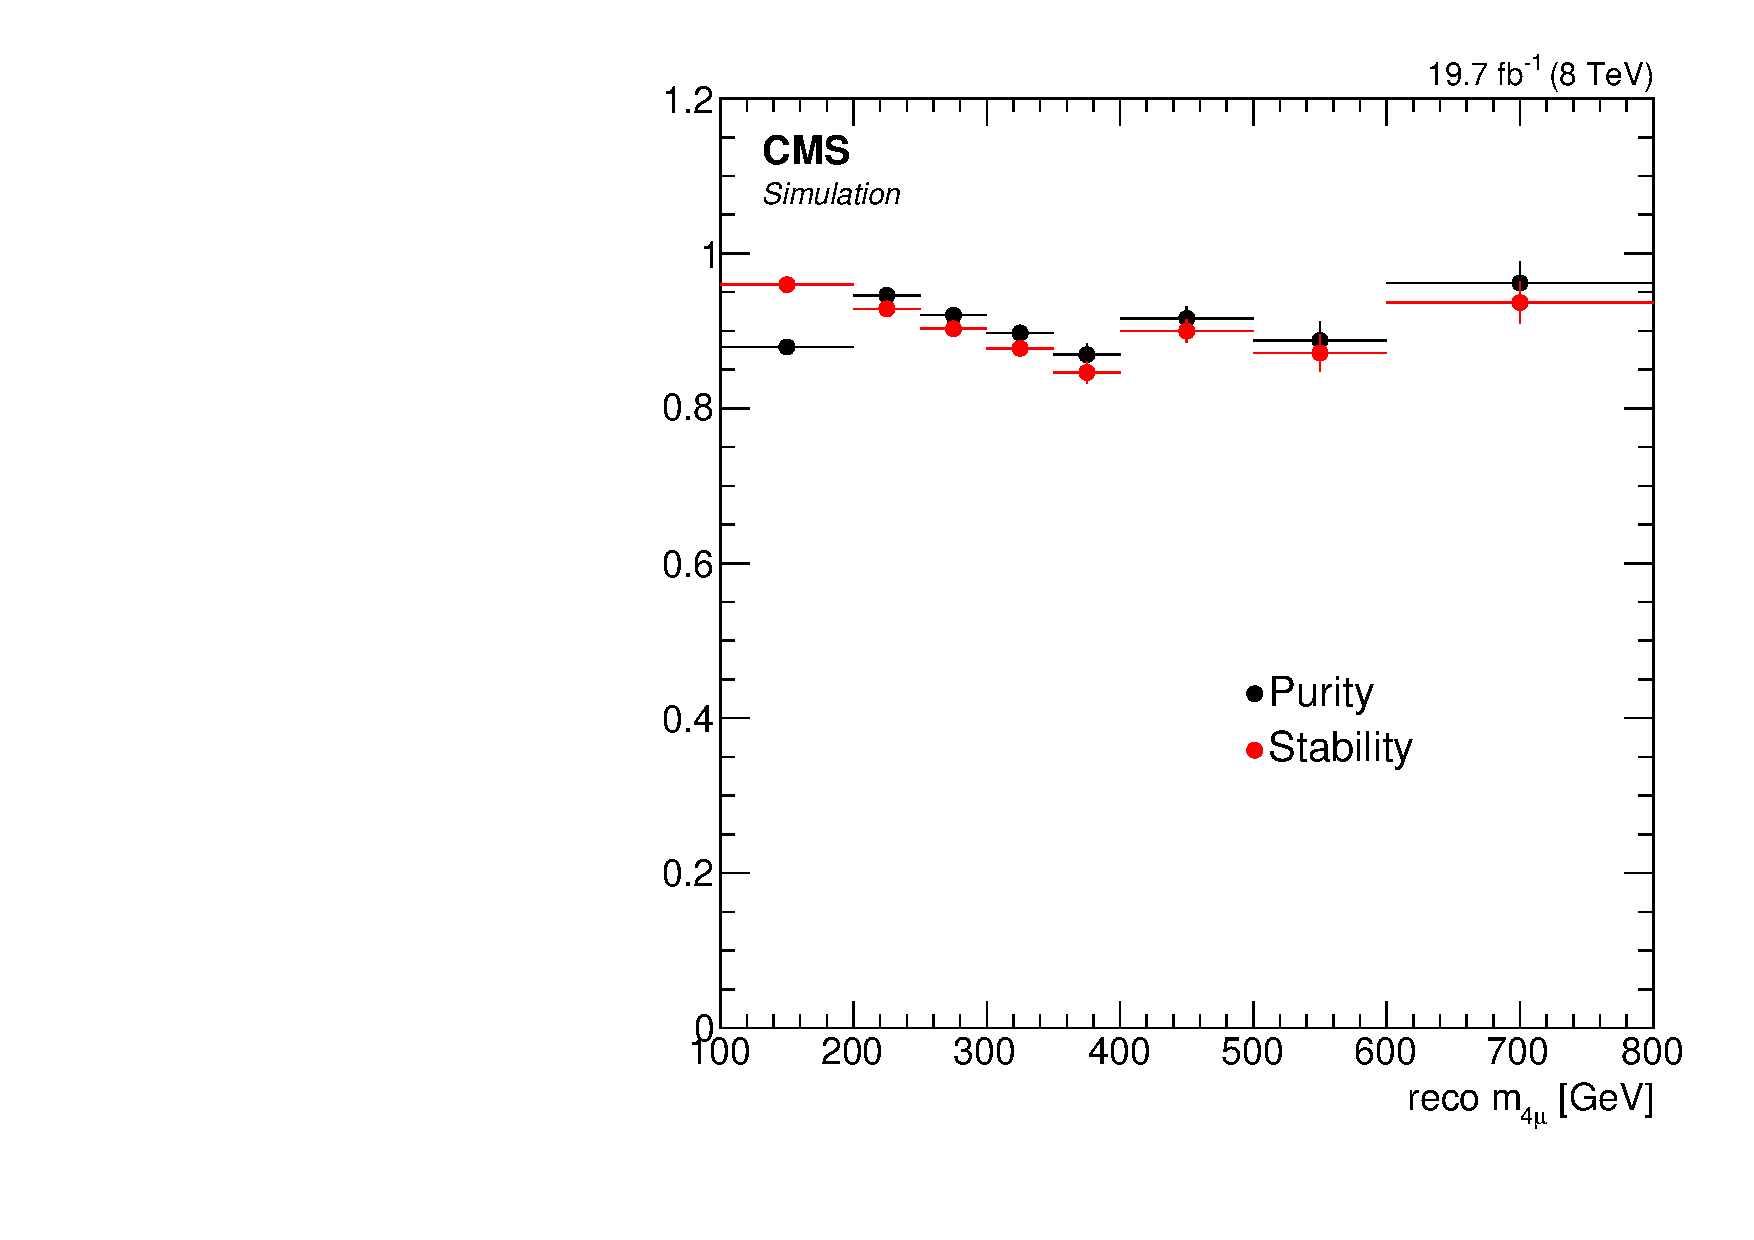
\includegraphics[width=0.8\cmsFigWidth]{Figures/Unfolding/BinMigration/PurityStability_4m_Mass_Pow}
    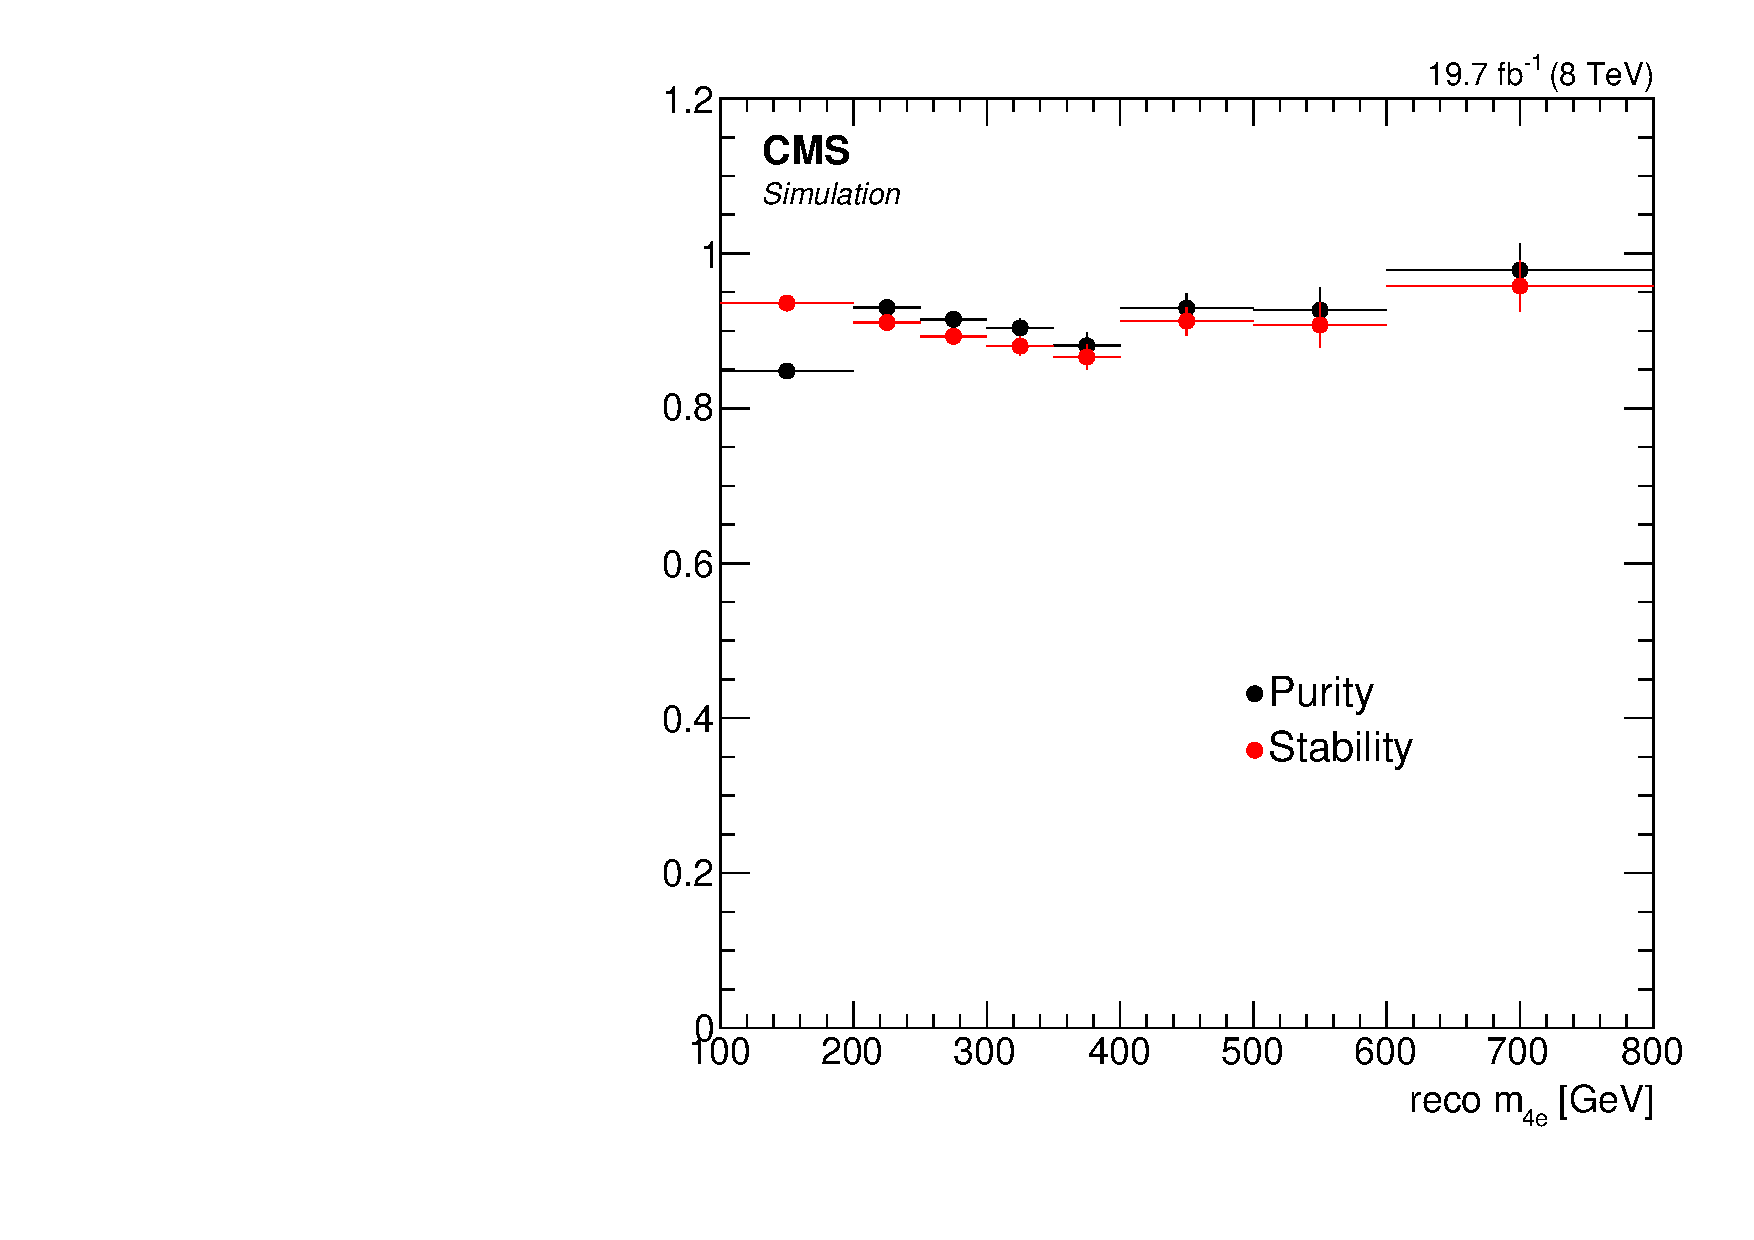
\includegraphics[width=0.8\cmsFigWidth]{Figures/Unfolding/BinMigration/PurityStability_4e_Mass_Pow}
    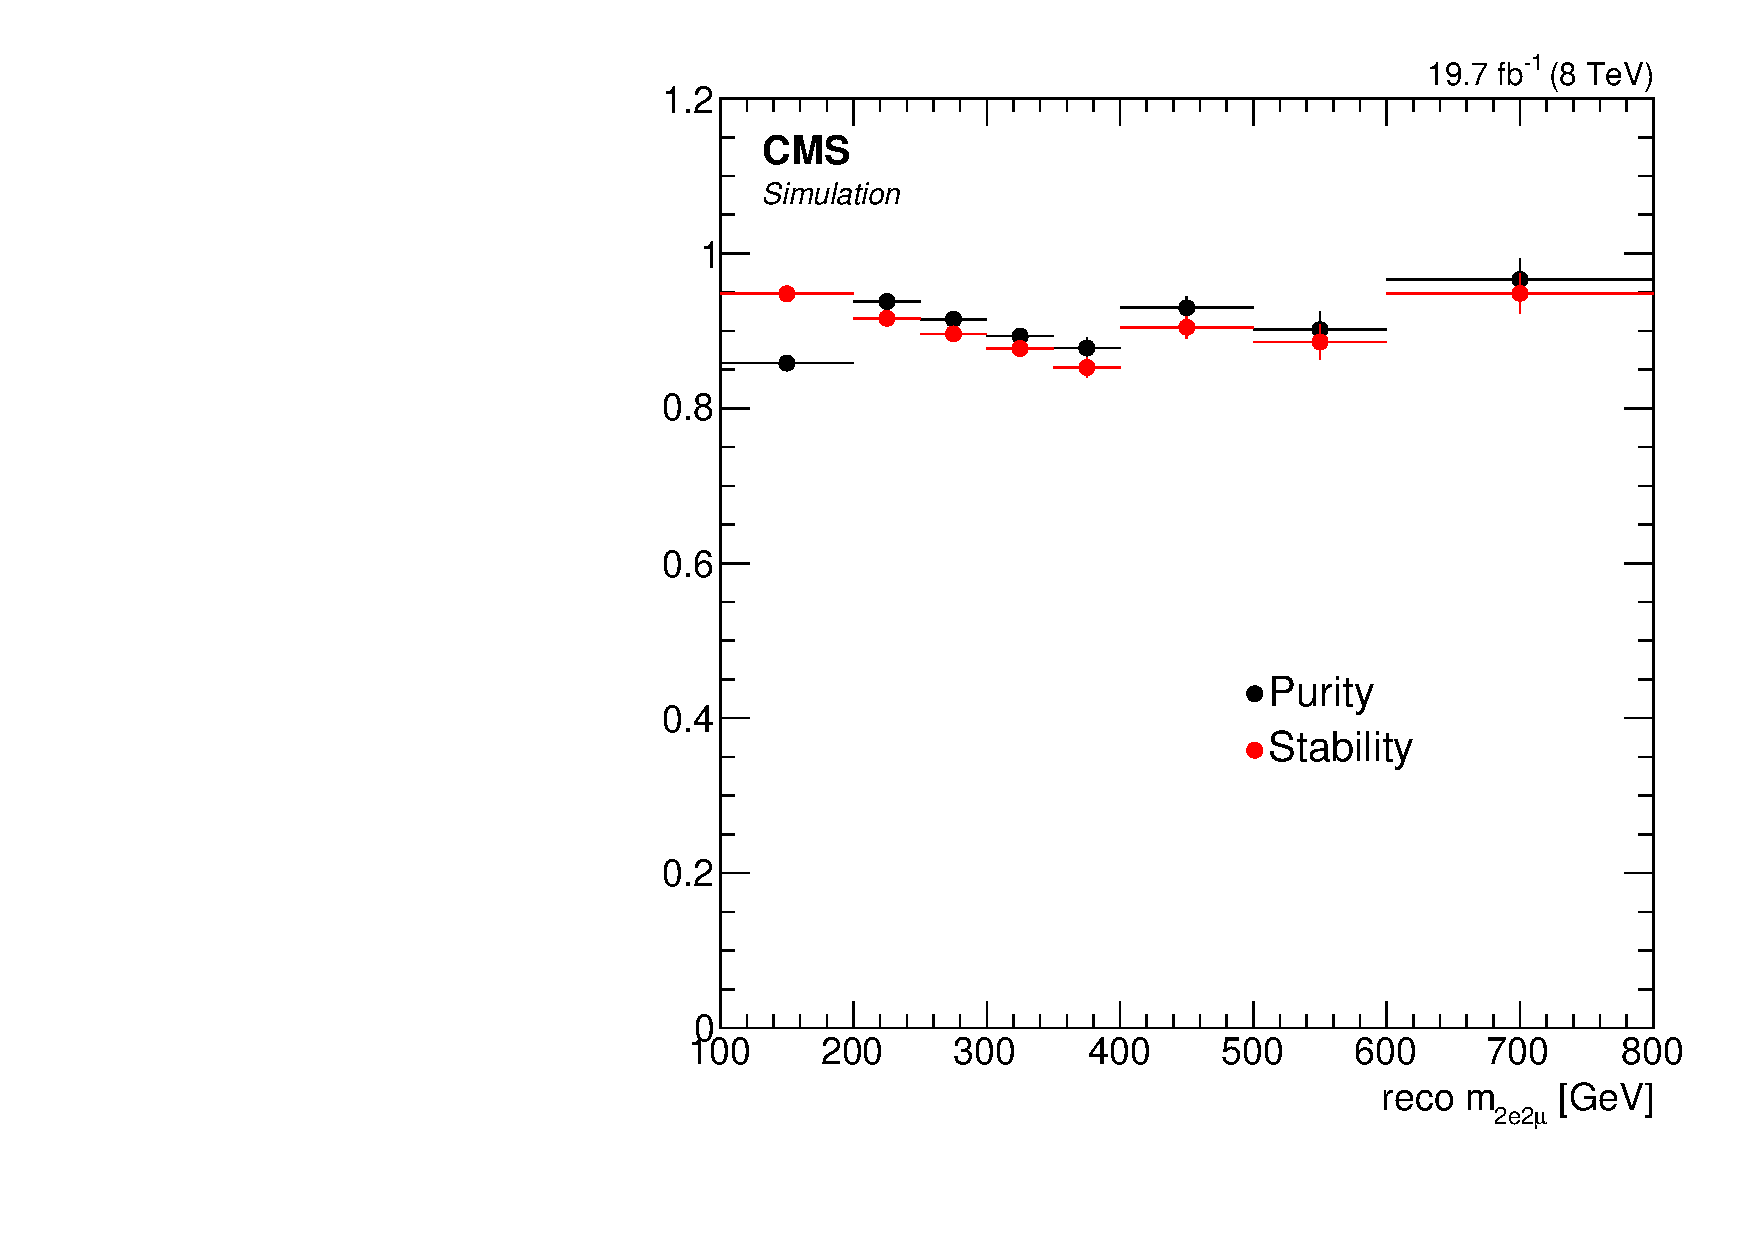
\includegraphics[width=0.8\cmsFigWidth]{Figures/Unfolding/BinMigration/PurityStability_2e2m_Mass_Pow}
    \caption{Purity and stability as a function of the 4-lepton invariant mass, for the $4\mu$ (left), $4e$ (center) and $2e2\mu$ (right) final states.}
    \label{fig:ps_mass}
  \end{center}
\end{figure}
\begin{figure}[hbtp]
  \begin{center}
    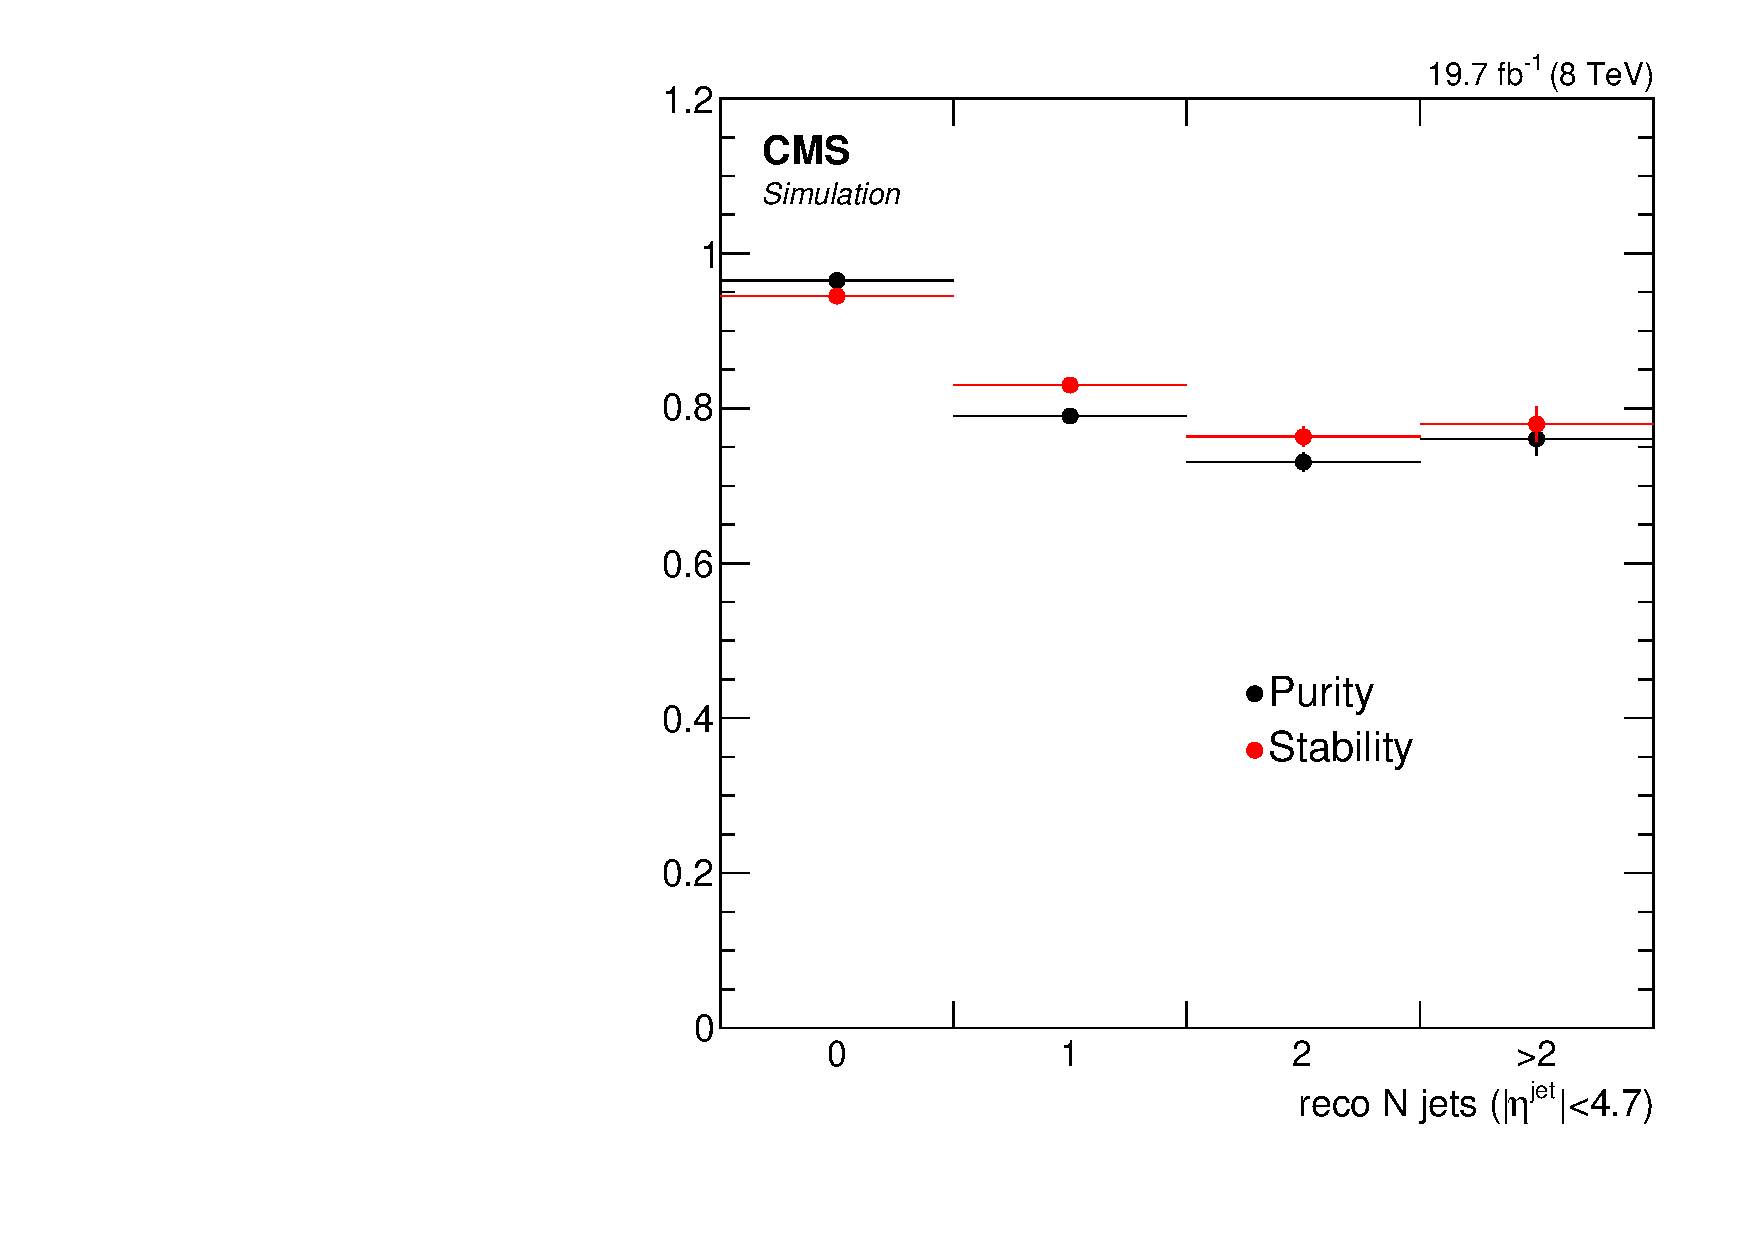
\includegraphics[width=0.8\cmsFigWidth]{Figures/Unfolding/BinMigration/PurityStability_4m_Jets_Mad}
    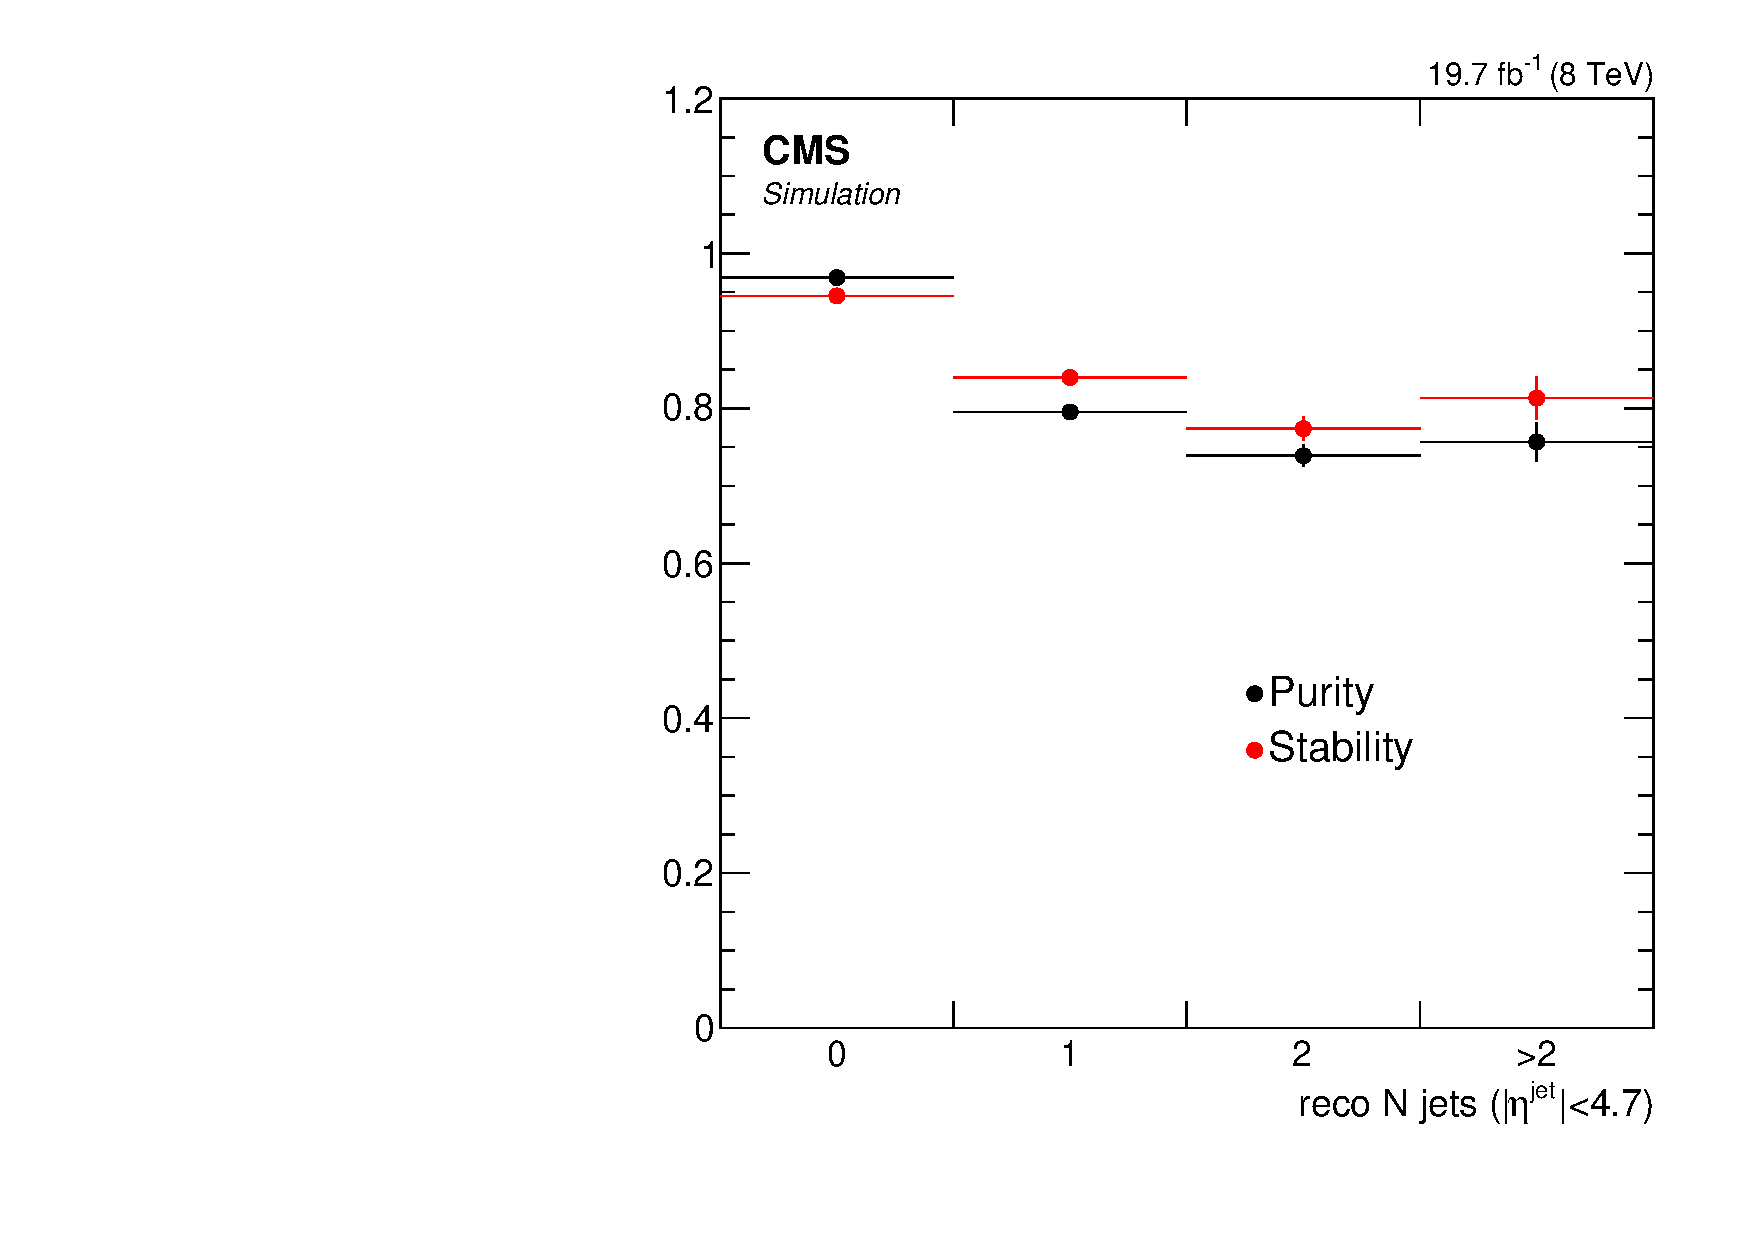
\includegraphics[width=0.8\cmsFigWidth]{Figures/Unfolding/BinMigration/PurityStability_4e_Jets_Mad}
    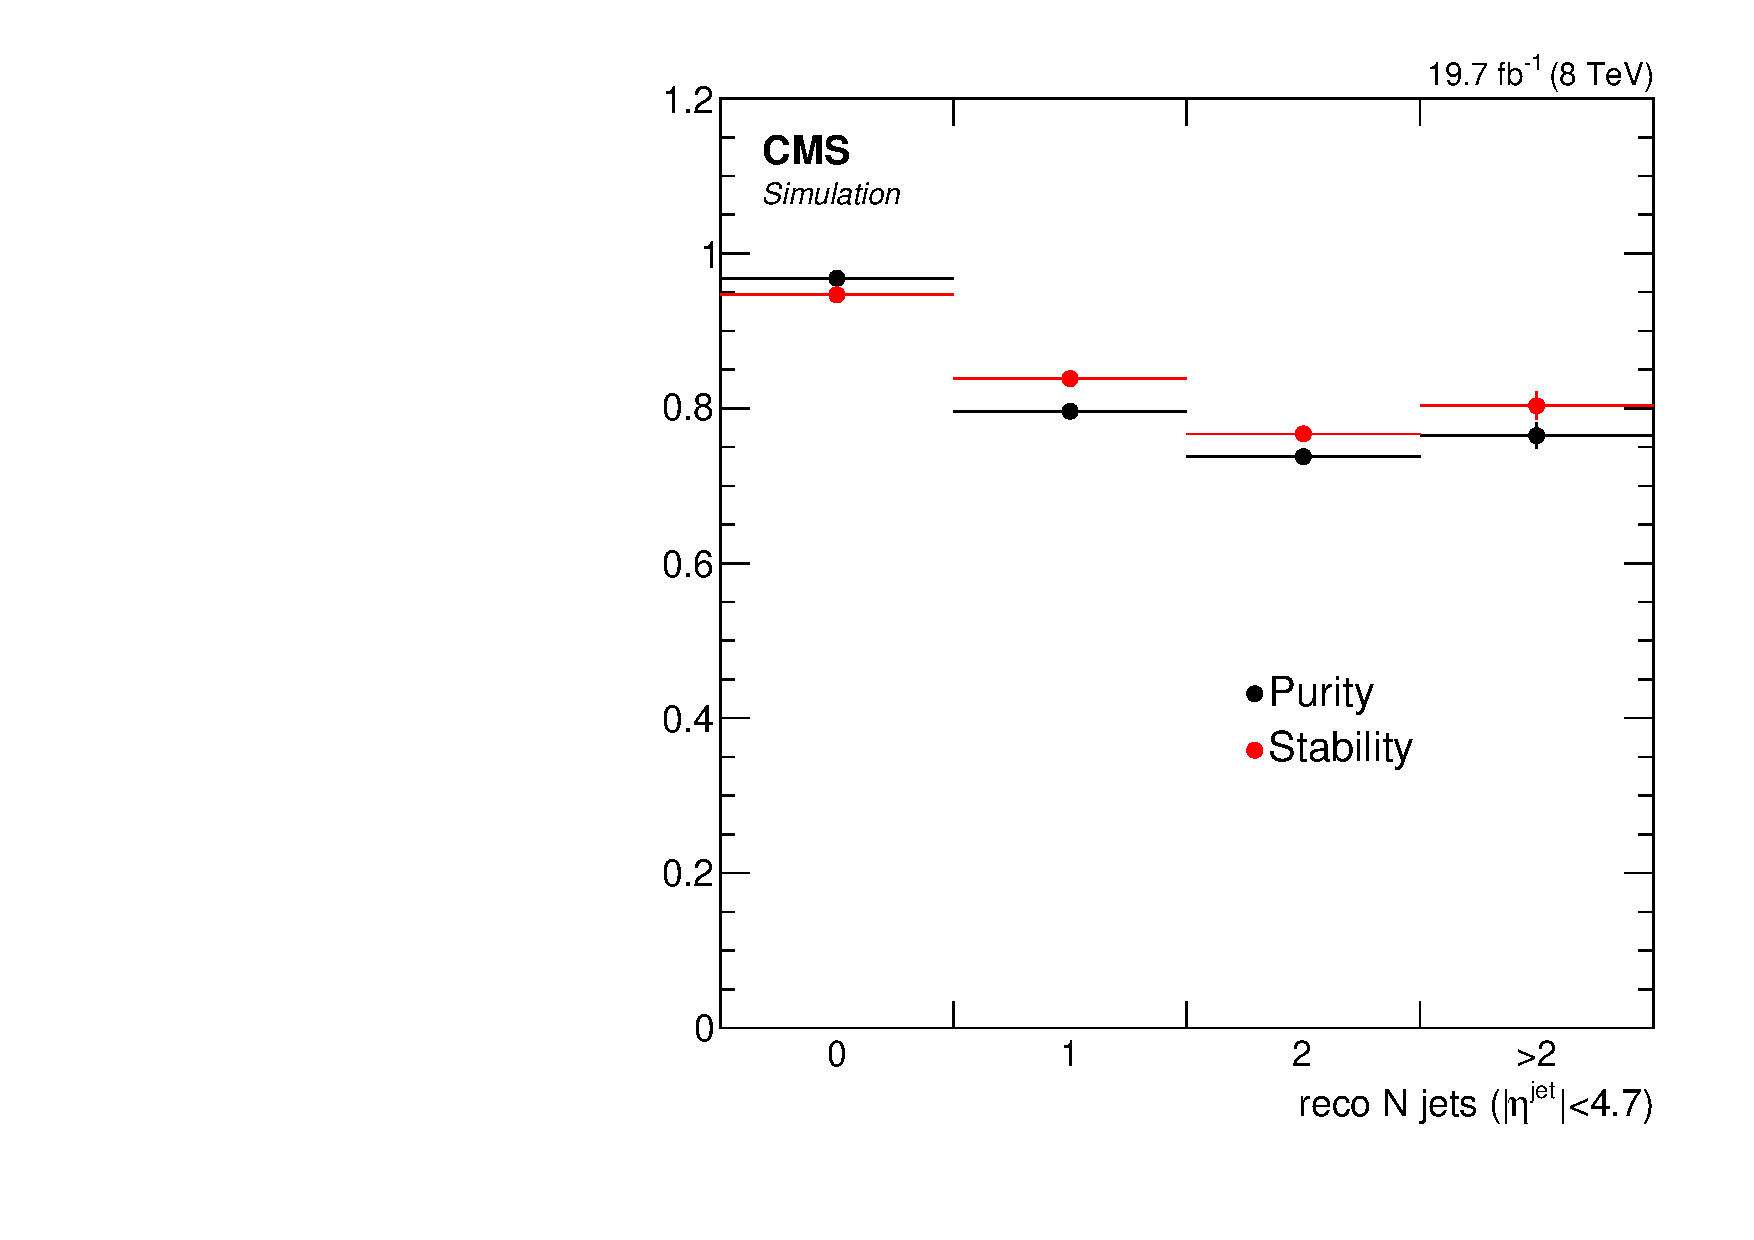
\includegraphics[width=0.8\cmsFigWidth]{Figures/Unfolding/BinMigration/PurityStability_2e2m_Jets_Mad}
    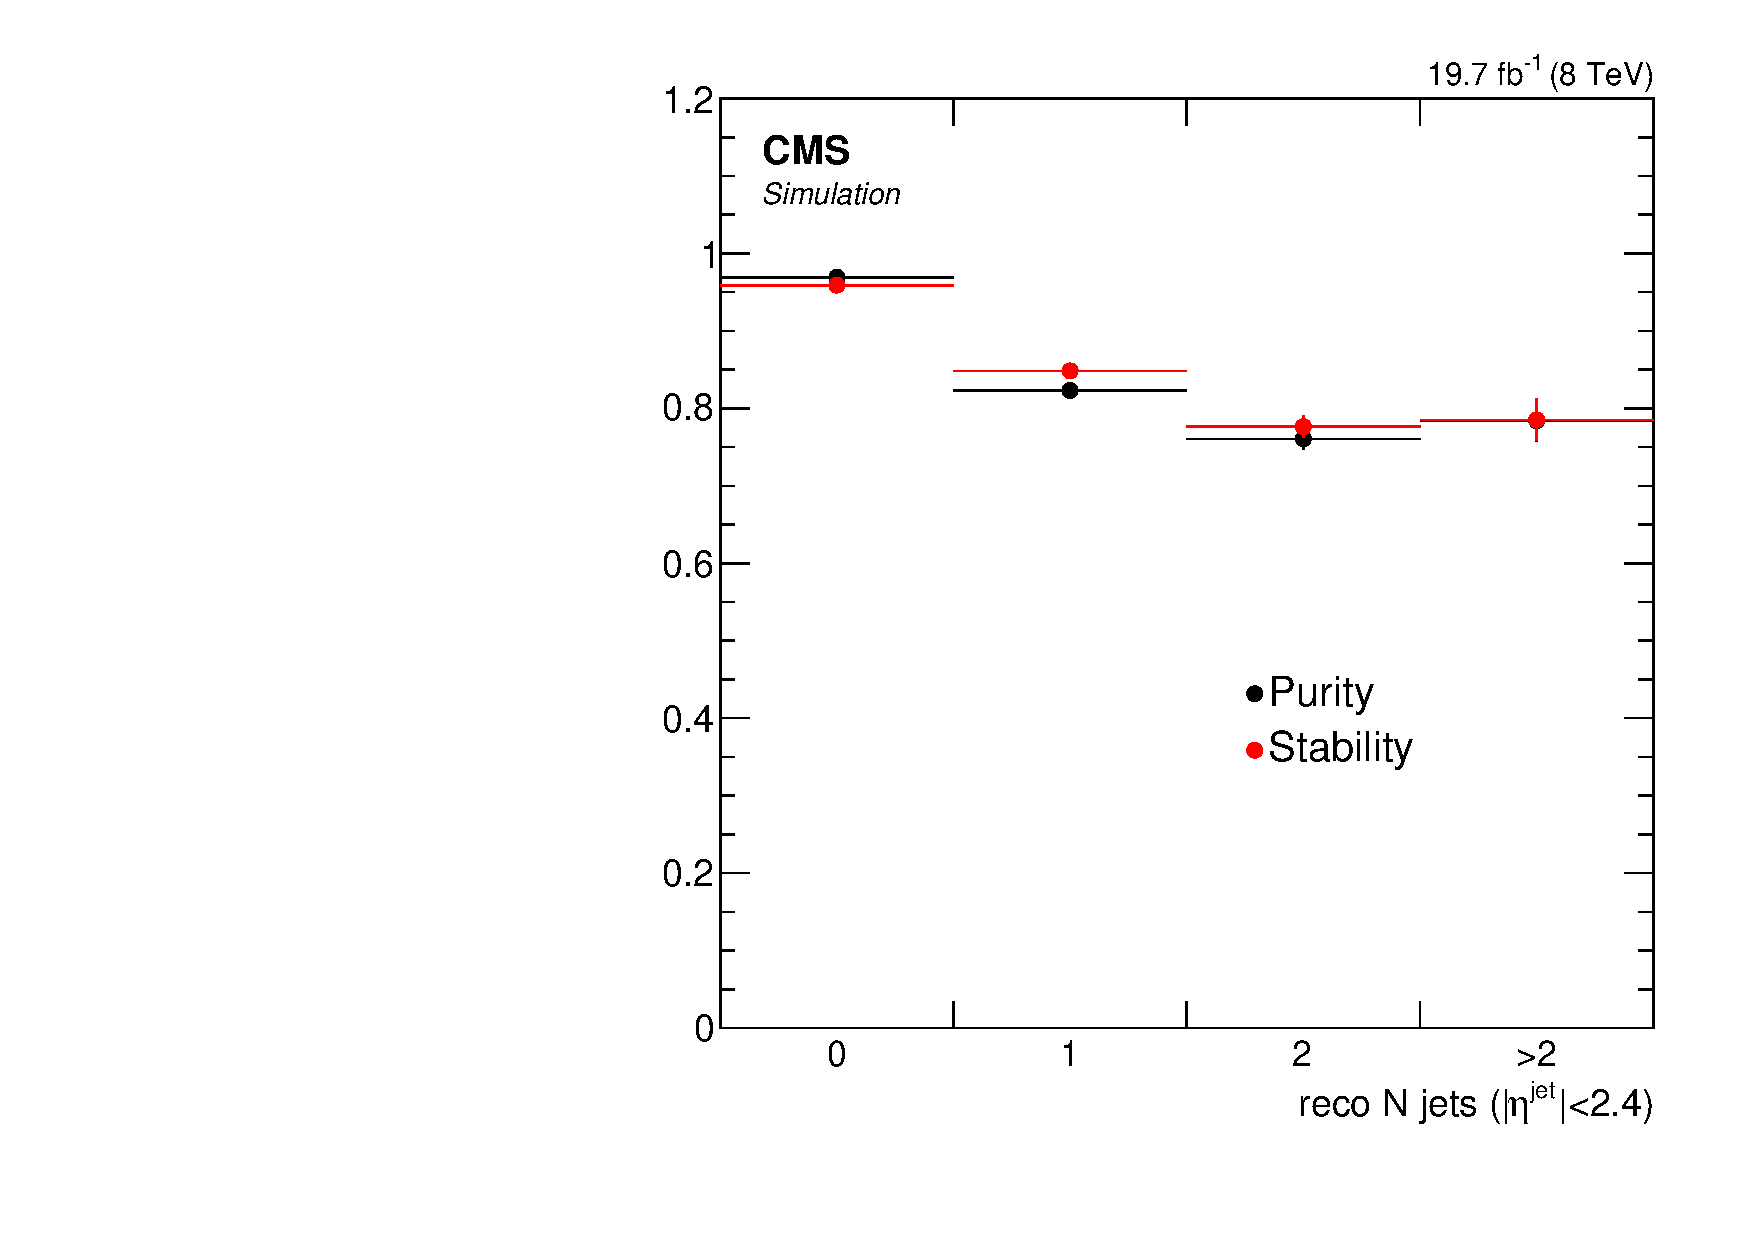
\includegraphics[width=0.8\cmsFigWidth]{Figures/Unfolding/BinMigration/PurityStability_4m_CentralJets_Mad}
    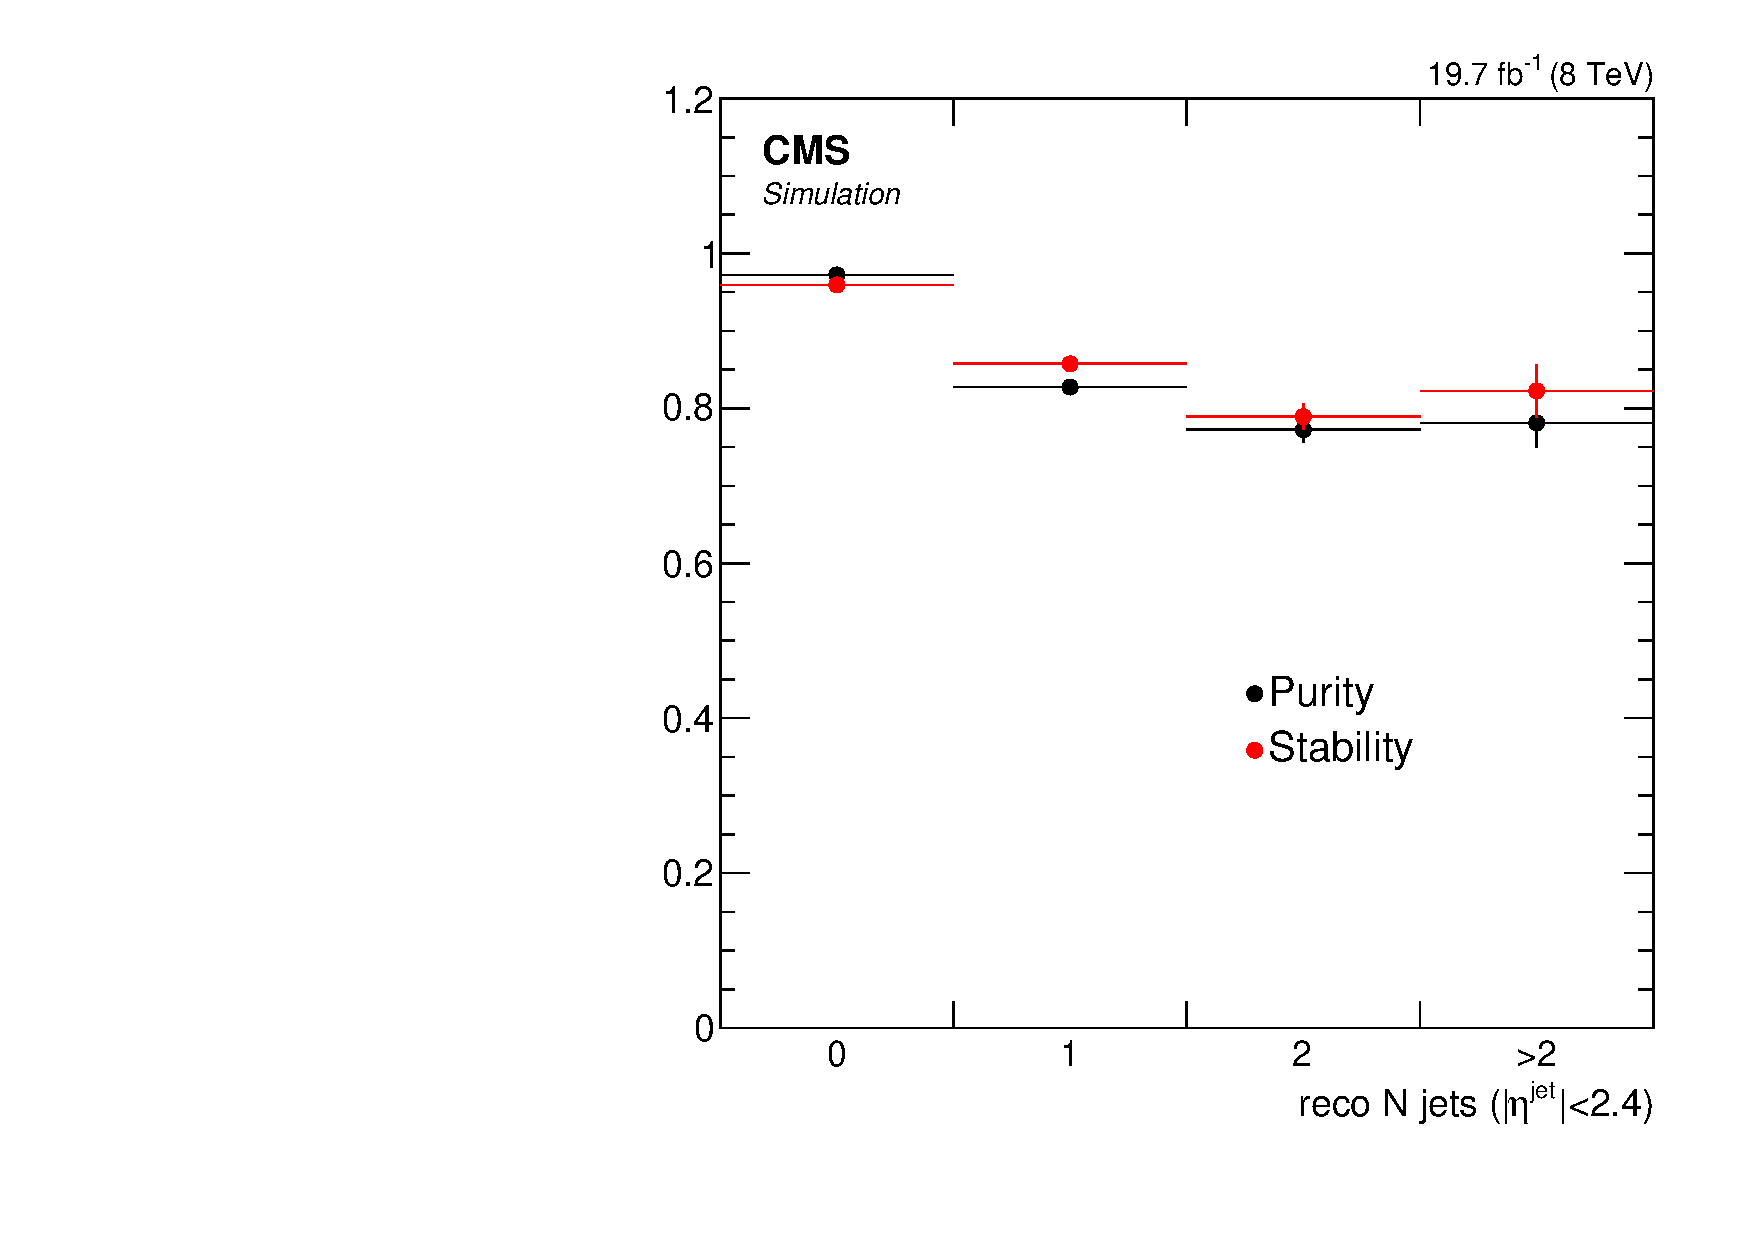
\includegraphics[width=0.8\cmsFigWidth]{Figures/Unfolding/BinMigration/PurityStability_4e_CentralJets_Mad}
    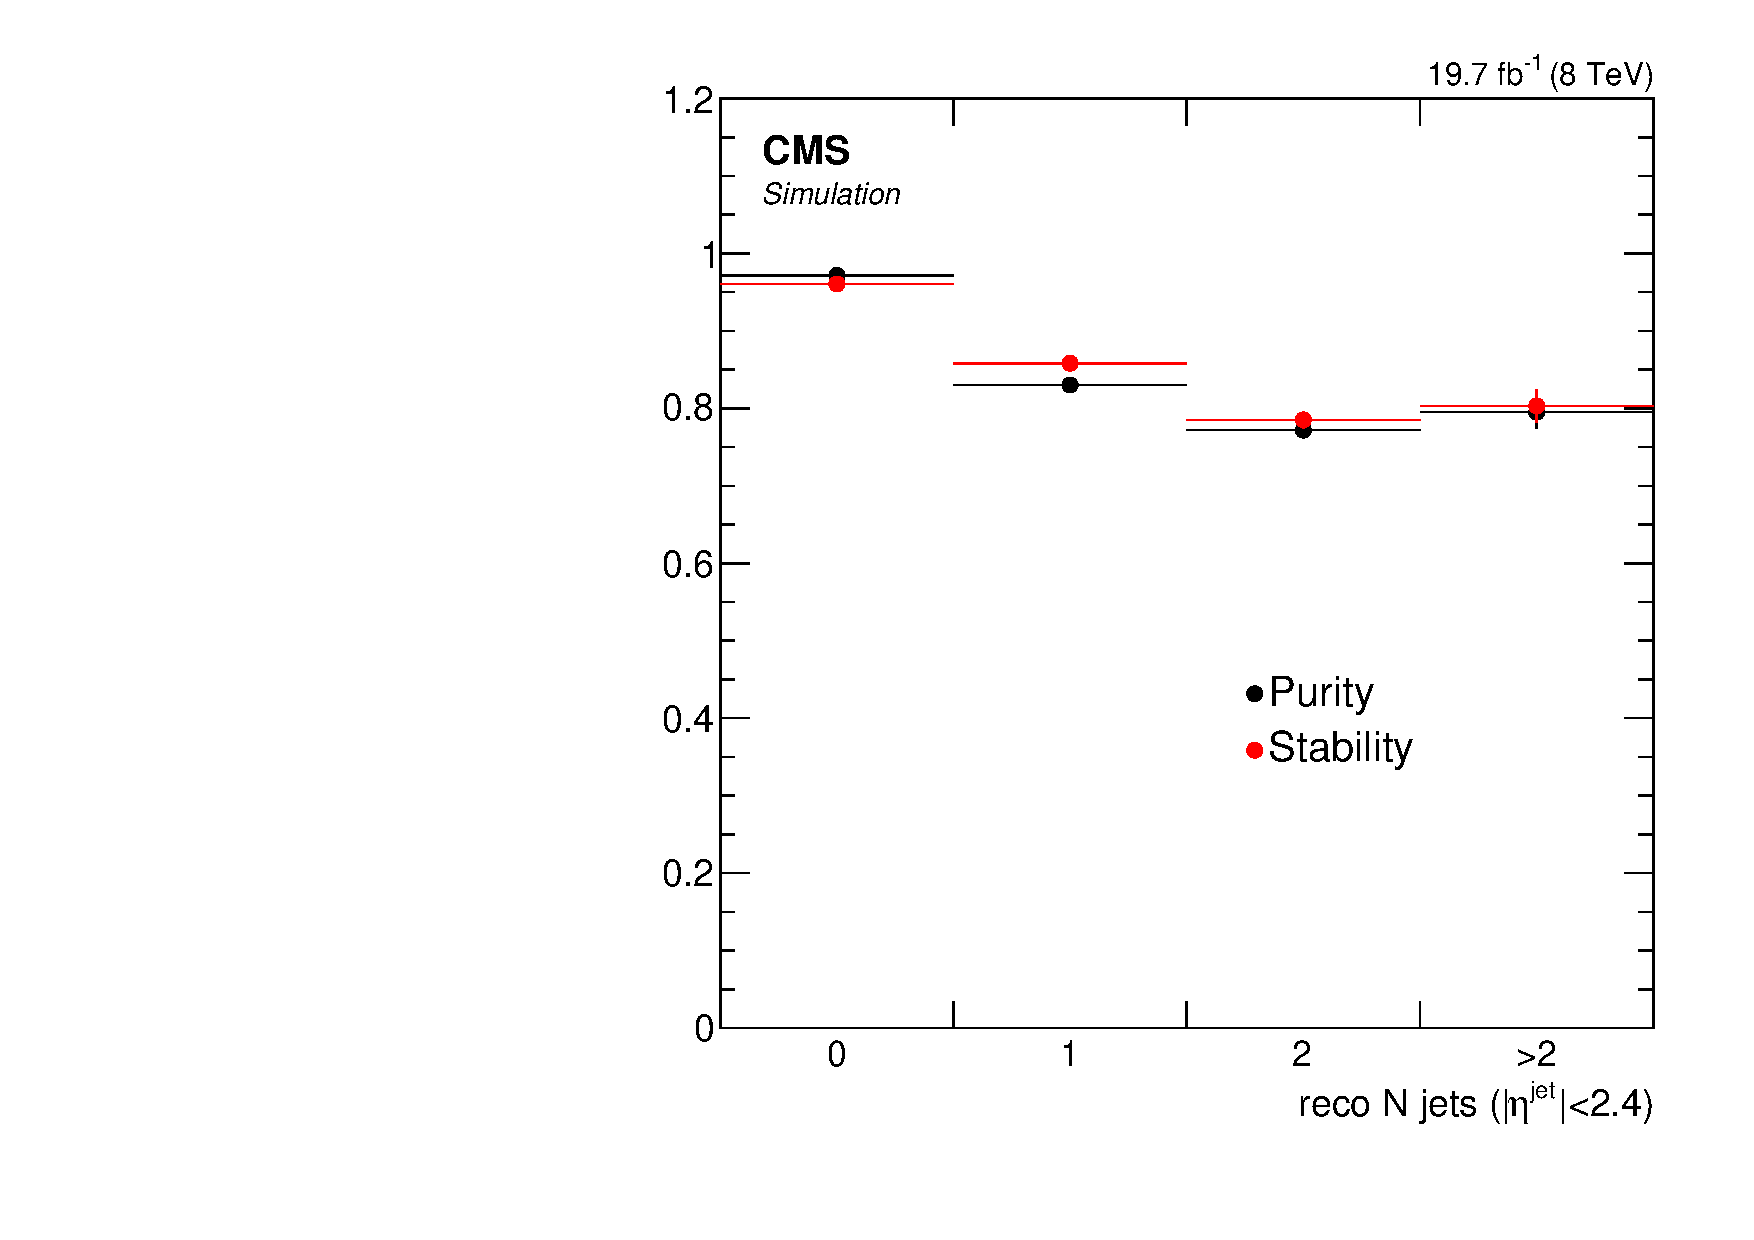
\includegraphics[width=0.8\cmsFigWidth]{Figures/Unfolding/BinMigration/PurityStability_2e2m_CentralJets_Mad}
 \caption{Purity and stability as a function of the number of jets (top) and central jets (bottom) in the event,  for the $4\mu$ (left), $4e$ (center) and $2e2\mu$ (right) final states.}
    \label{fig:ps_jets}
  \end{center}
\end{figure}
\begin{figure}[hbtp]
  \begin{center}
    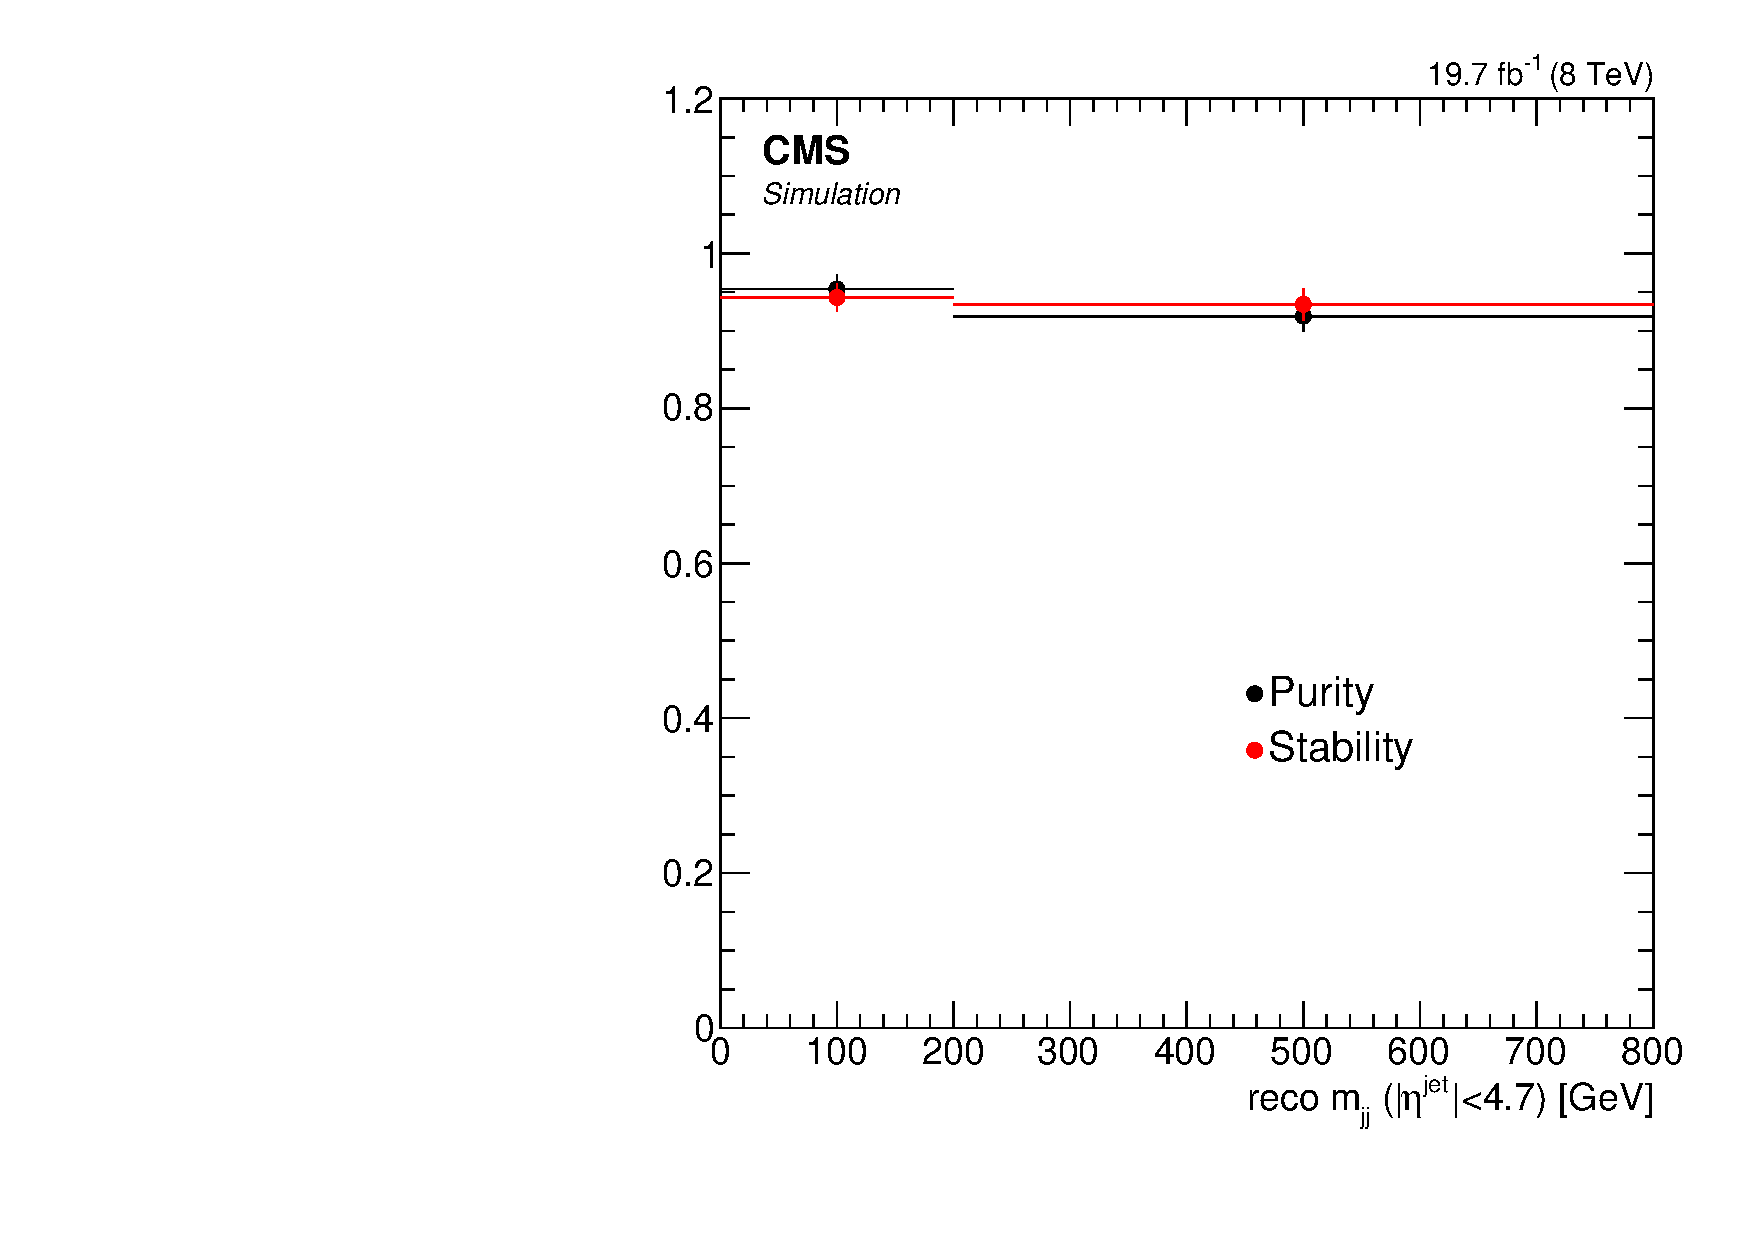
\includegraphics[width=0.8\cmsFigWidth]{Figures/Unfolding/BinMigration/PurityStability_4m_Mjj_Mad}
    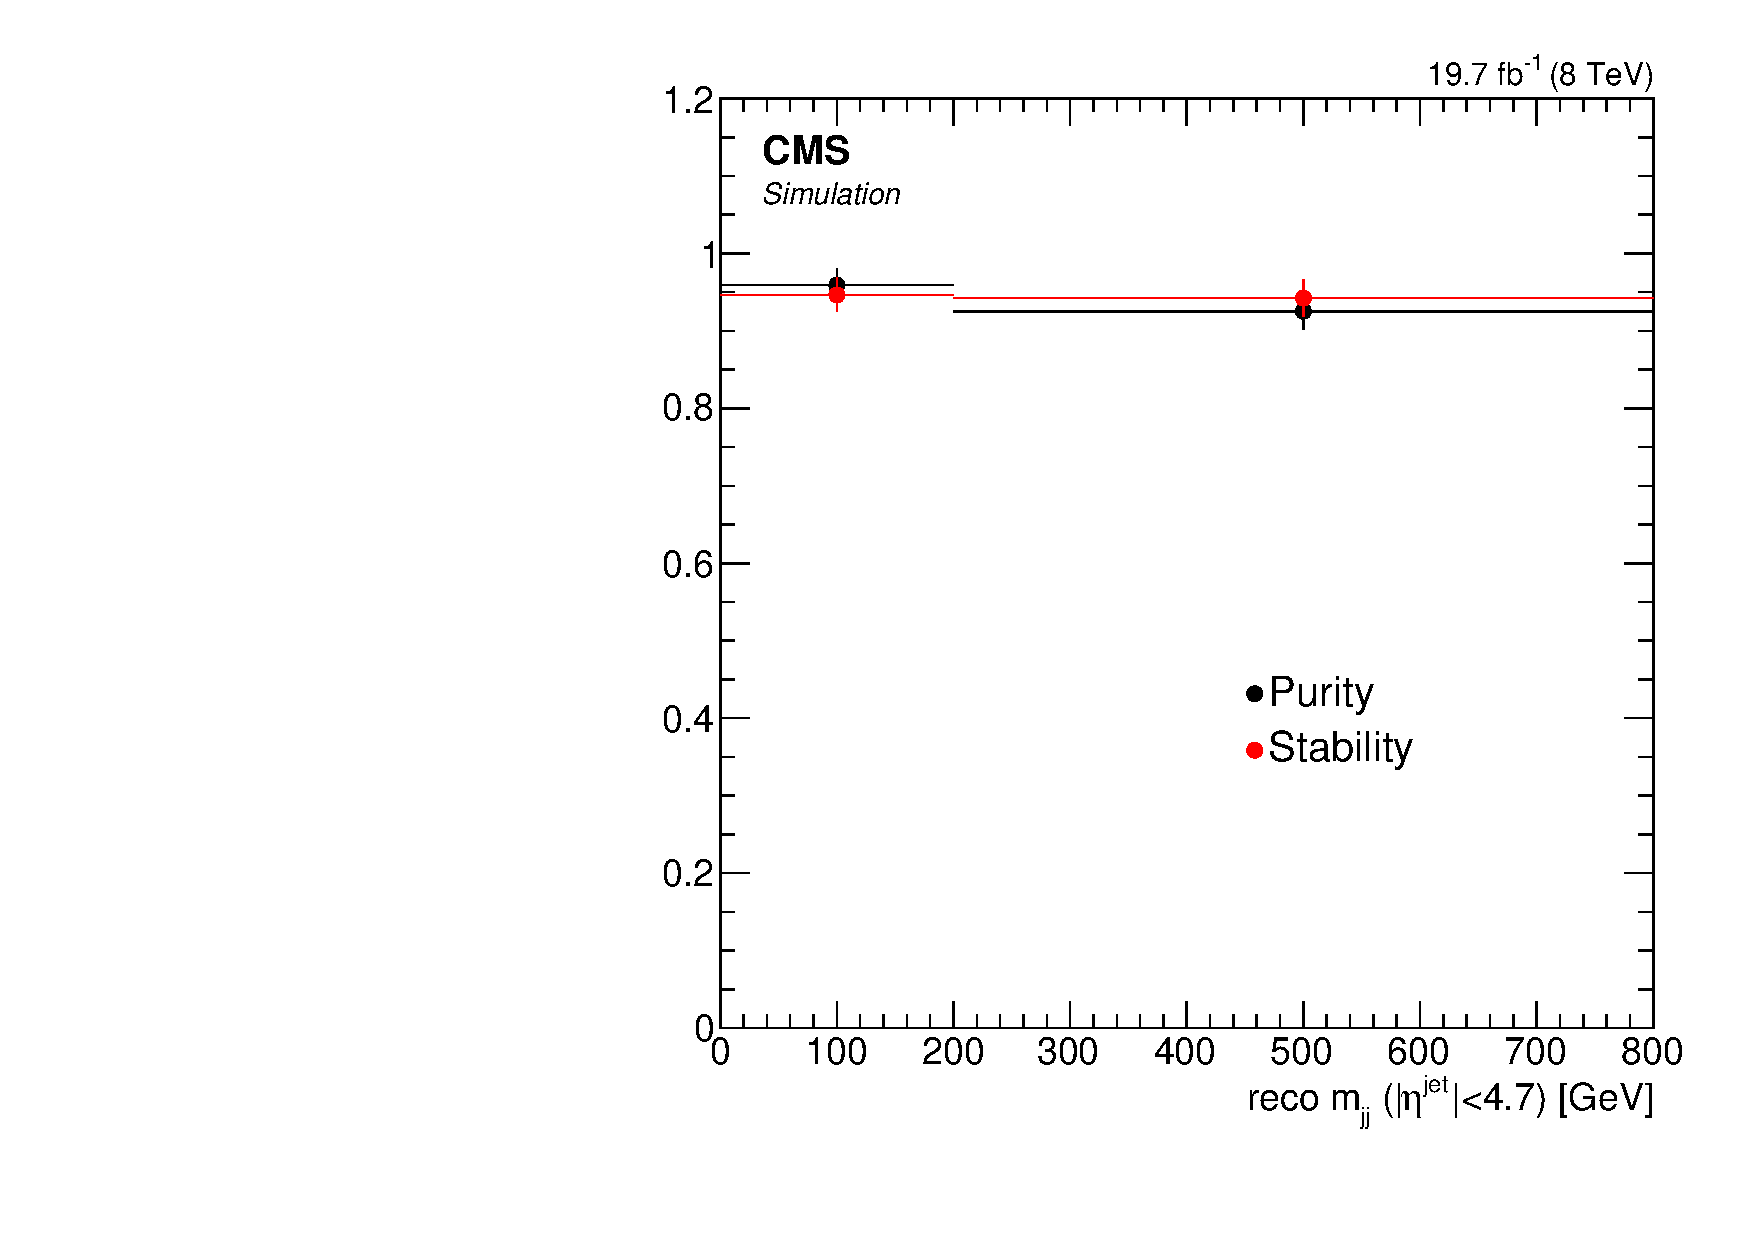
\includegraphics[width=0.8\cmsFigWidth]{Figures/Unfolding/BinMigration/PurityStability_4e_Mjj_Mad}
    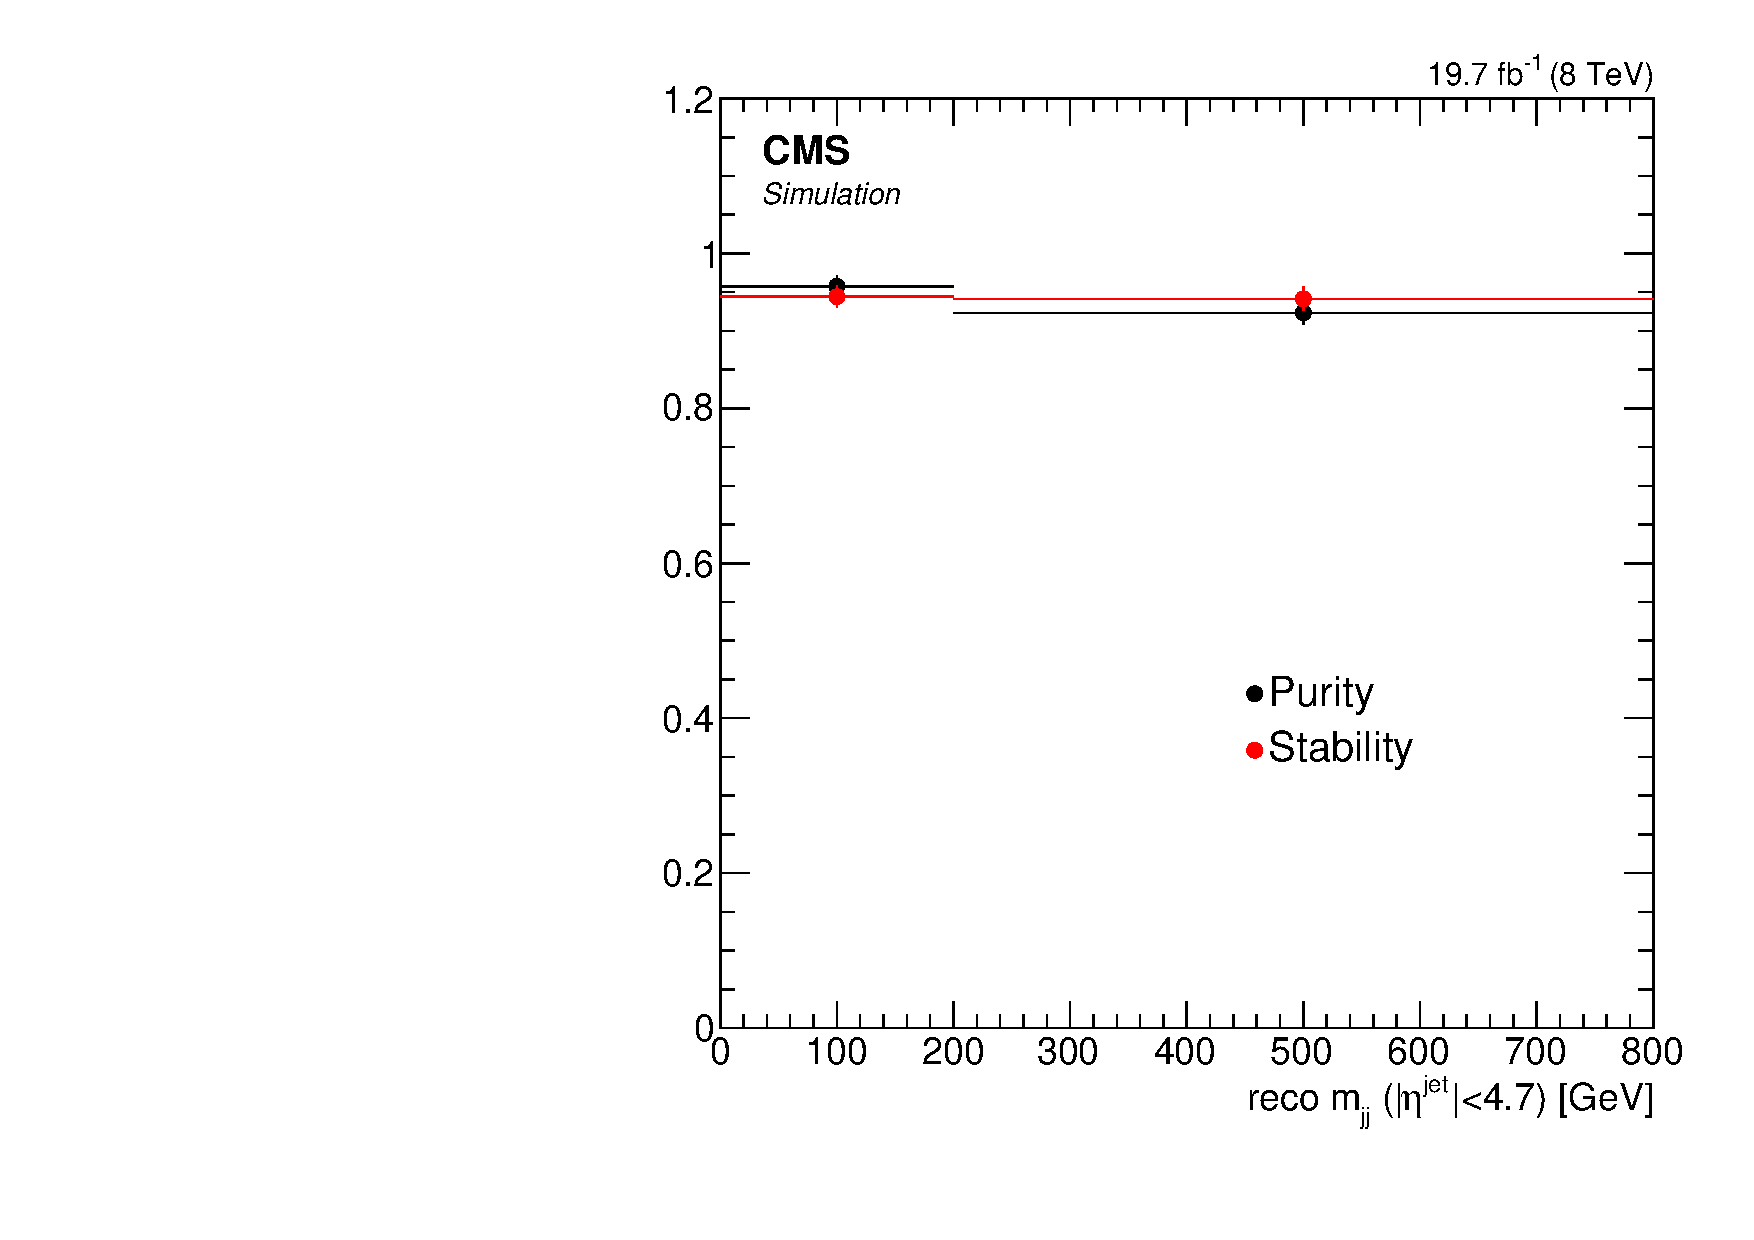
\includegraphics[width=0.8\cmsFigWidth]{Figures/Unfolding/BinMigration/PurityStability_2e2m_Mjj_Mad}
    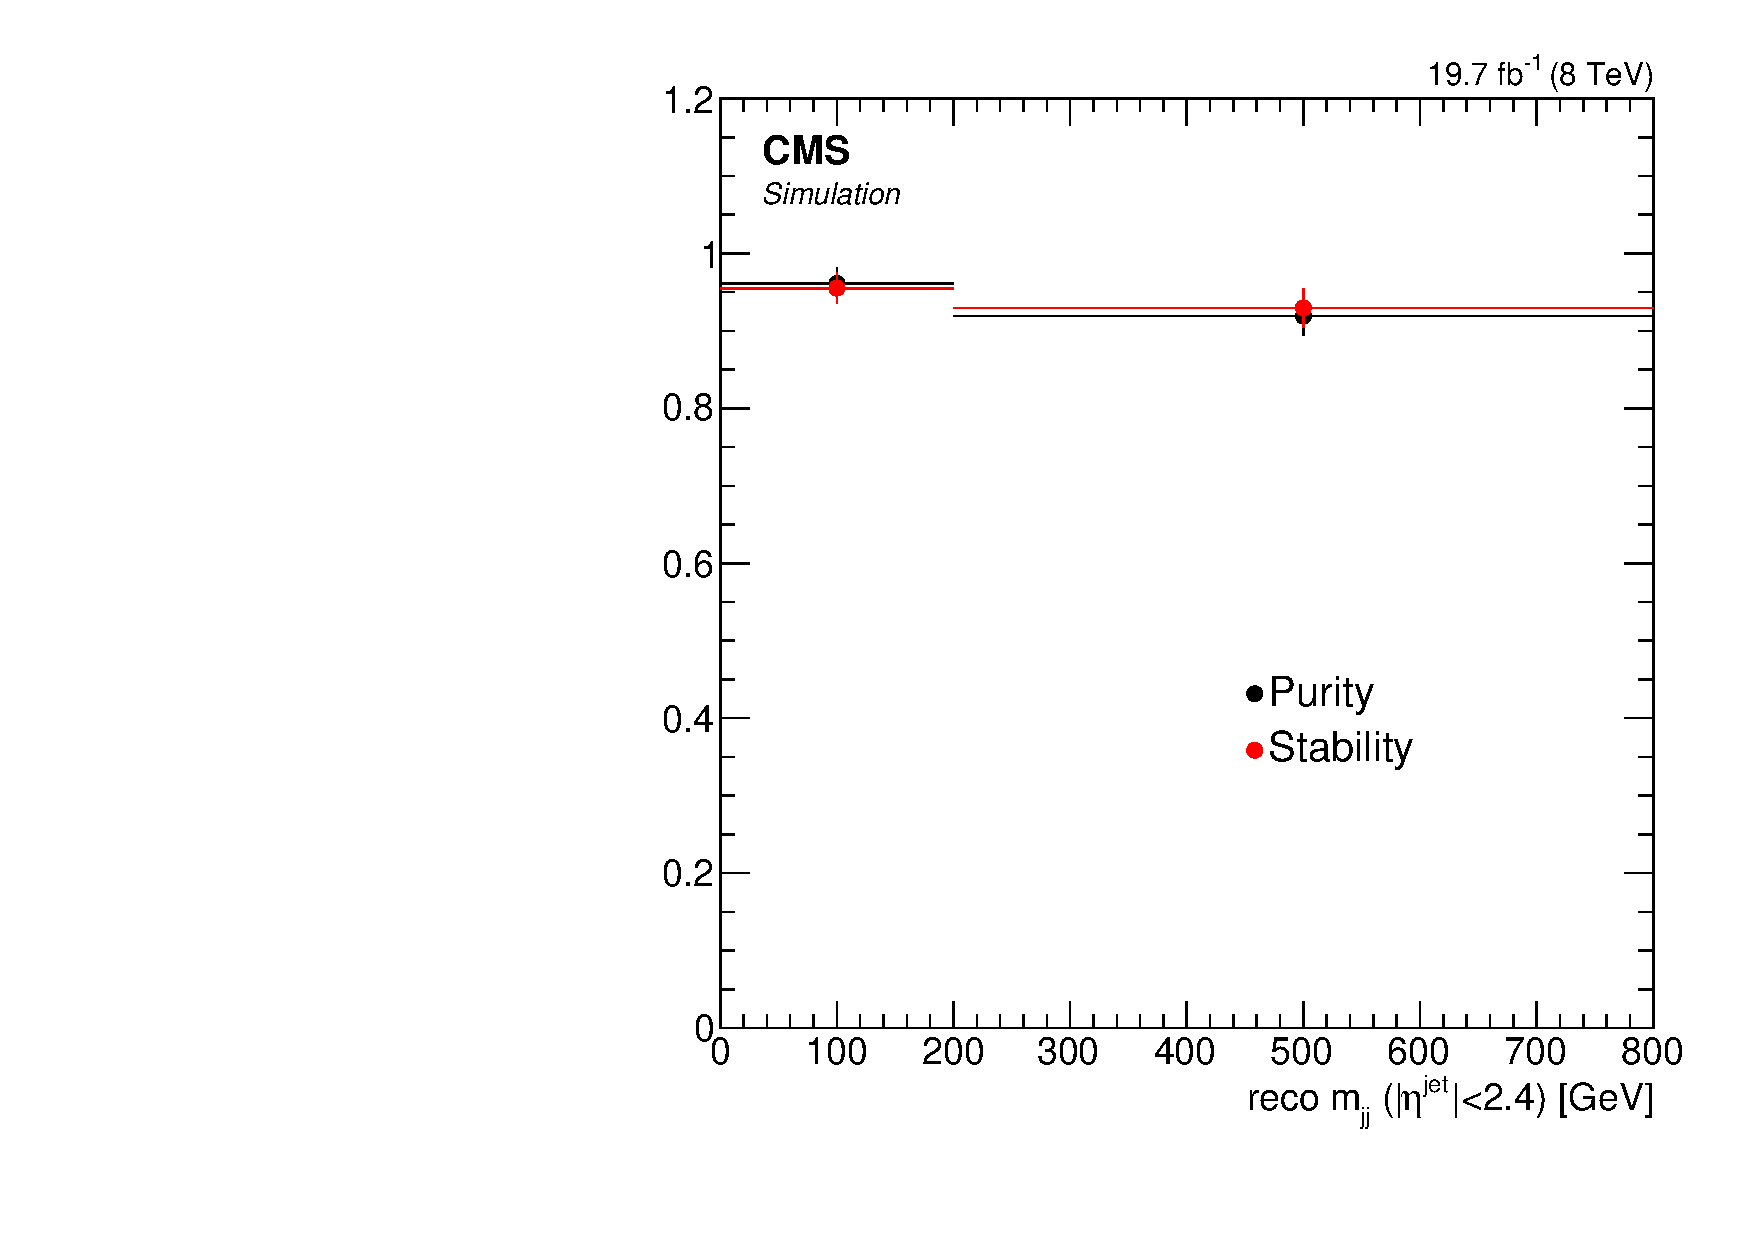
\includegraphics[width=0.8\cmsFigWidth]{Figures/Unfolding/BinMigration/PurityStability_4m_CentralMjj_Mad}
    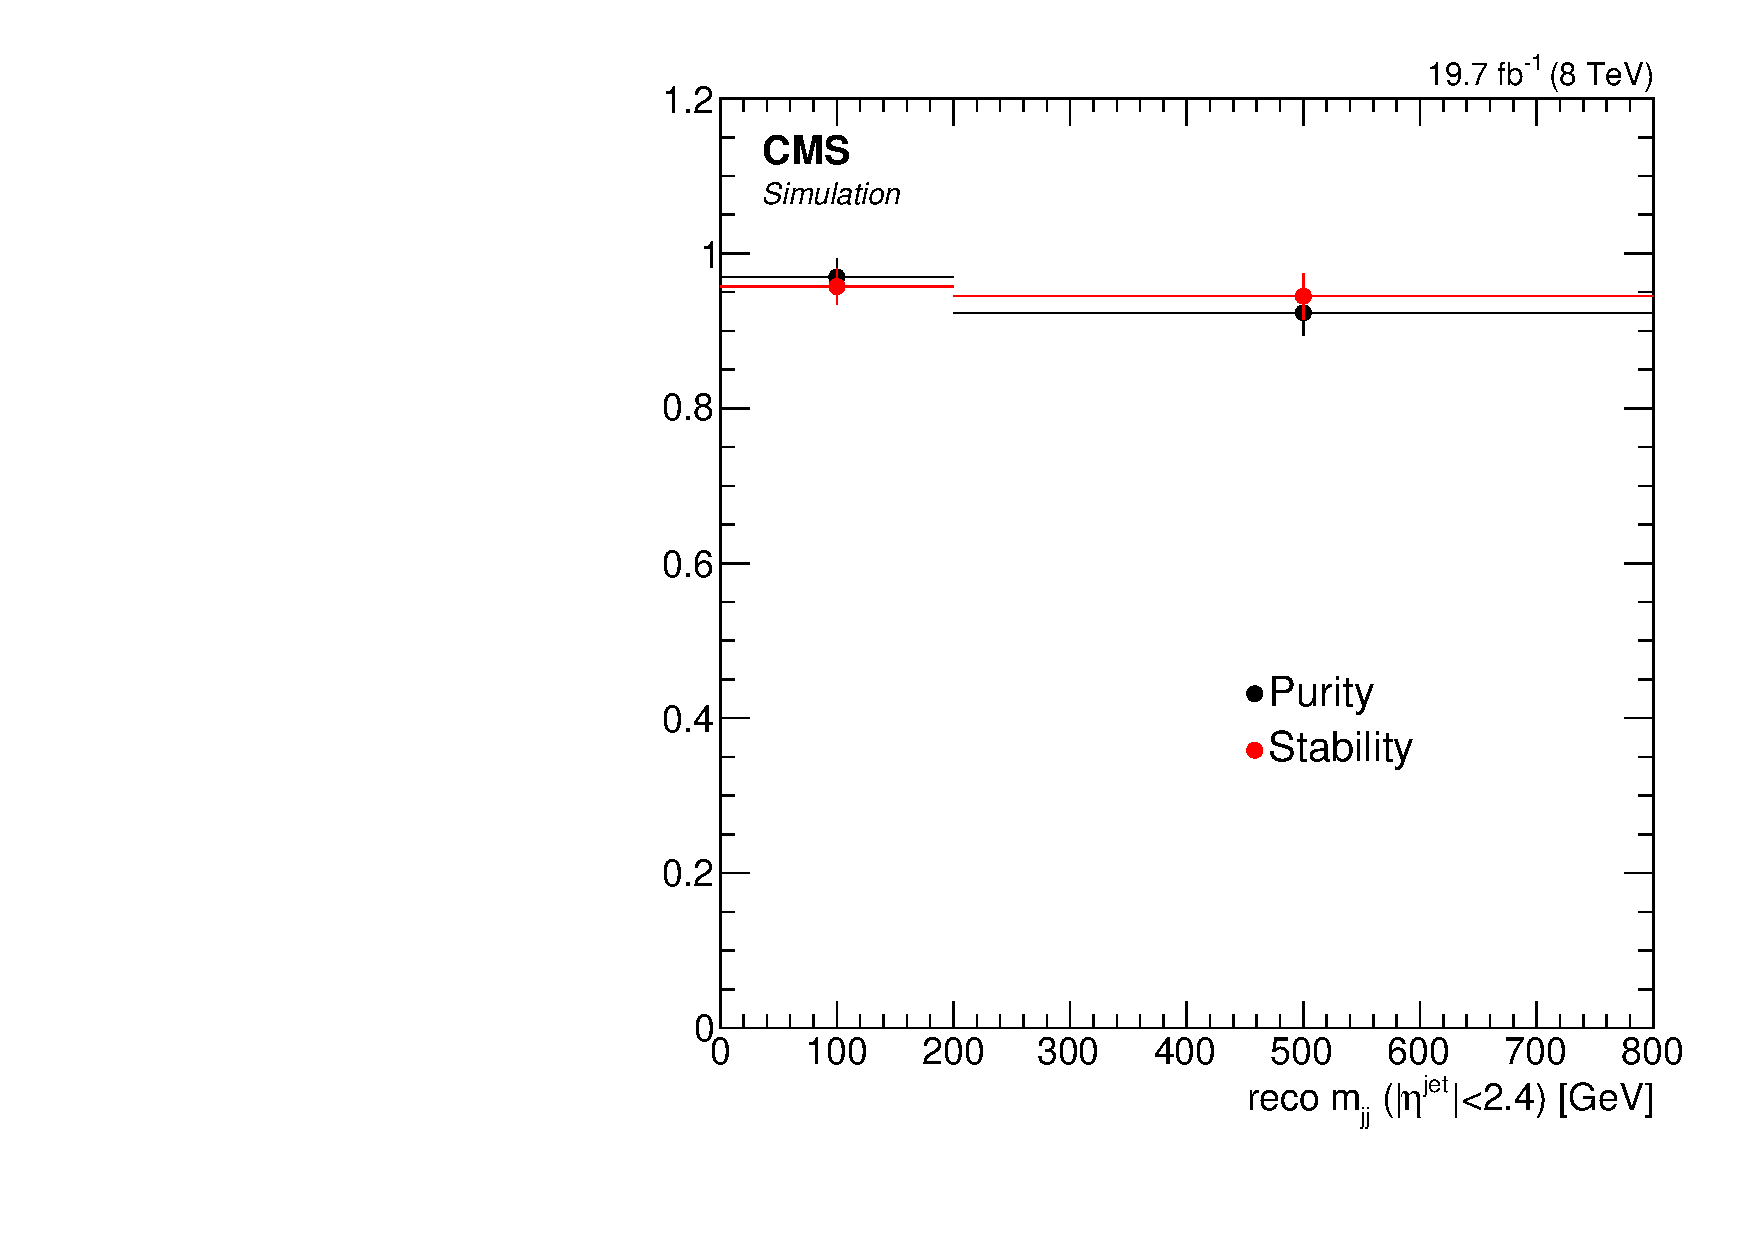
\includegraphics[width=0.8\cmsFigWidth]{Figures/Unfolding/BinMigration/PurityStability_4e_CentralMjj_Mad}
    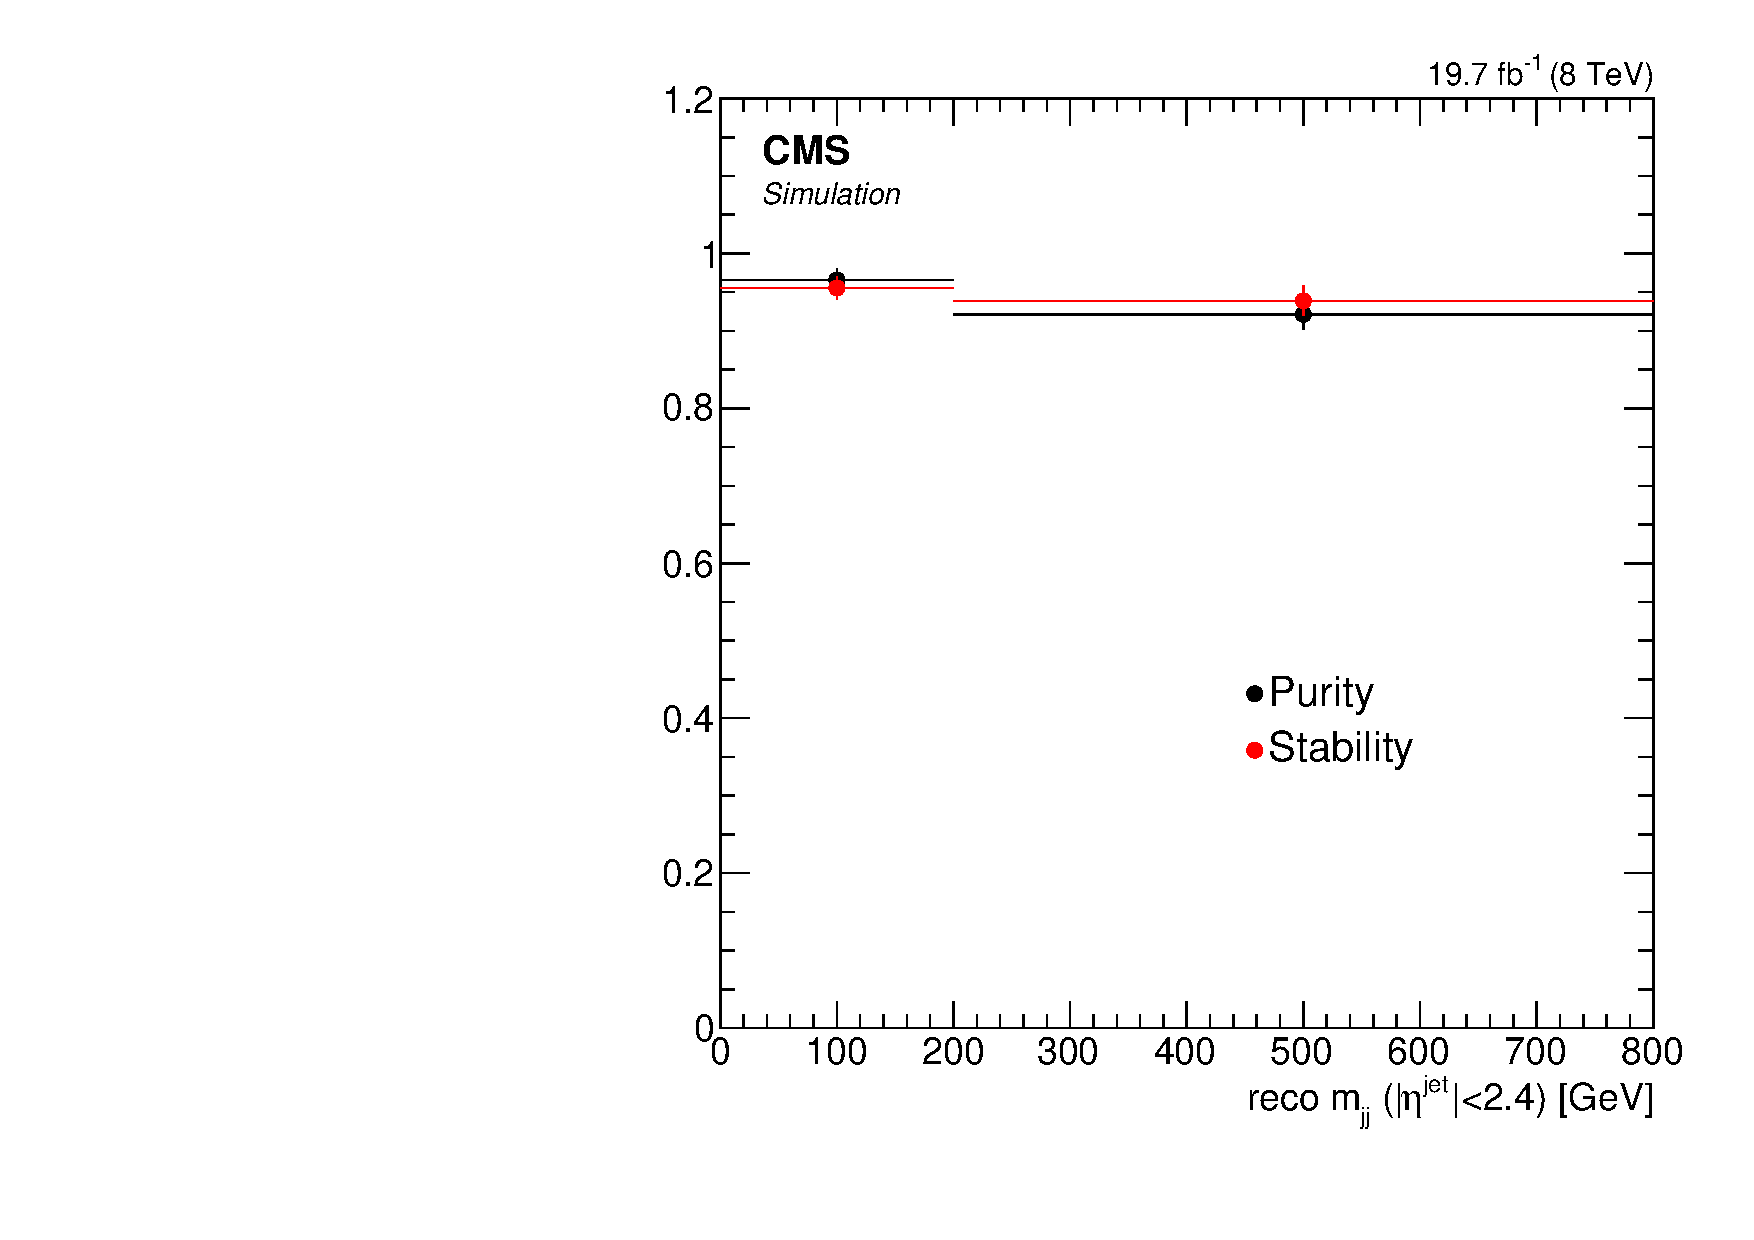
\includegraphics[width=0.8\cmsFigWidth]{Figures/Unfolding/BinMigration/PurityStability_2e2m_CentralMjj_Mad}
 \caption{Purity and stability as a function of the invariant mass of the two most energetic jets (top) and  central jets (bottom) in the event,  for the $4\mu$ (left), $4e$ (center) and $2e2\mu$ (right) final states.}
    \label{fig:ps_mjj}
  \end{center}
\end{figure}
\begin{figure}[hbtp]
  \begin{center}
    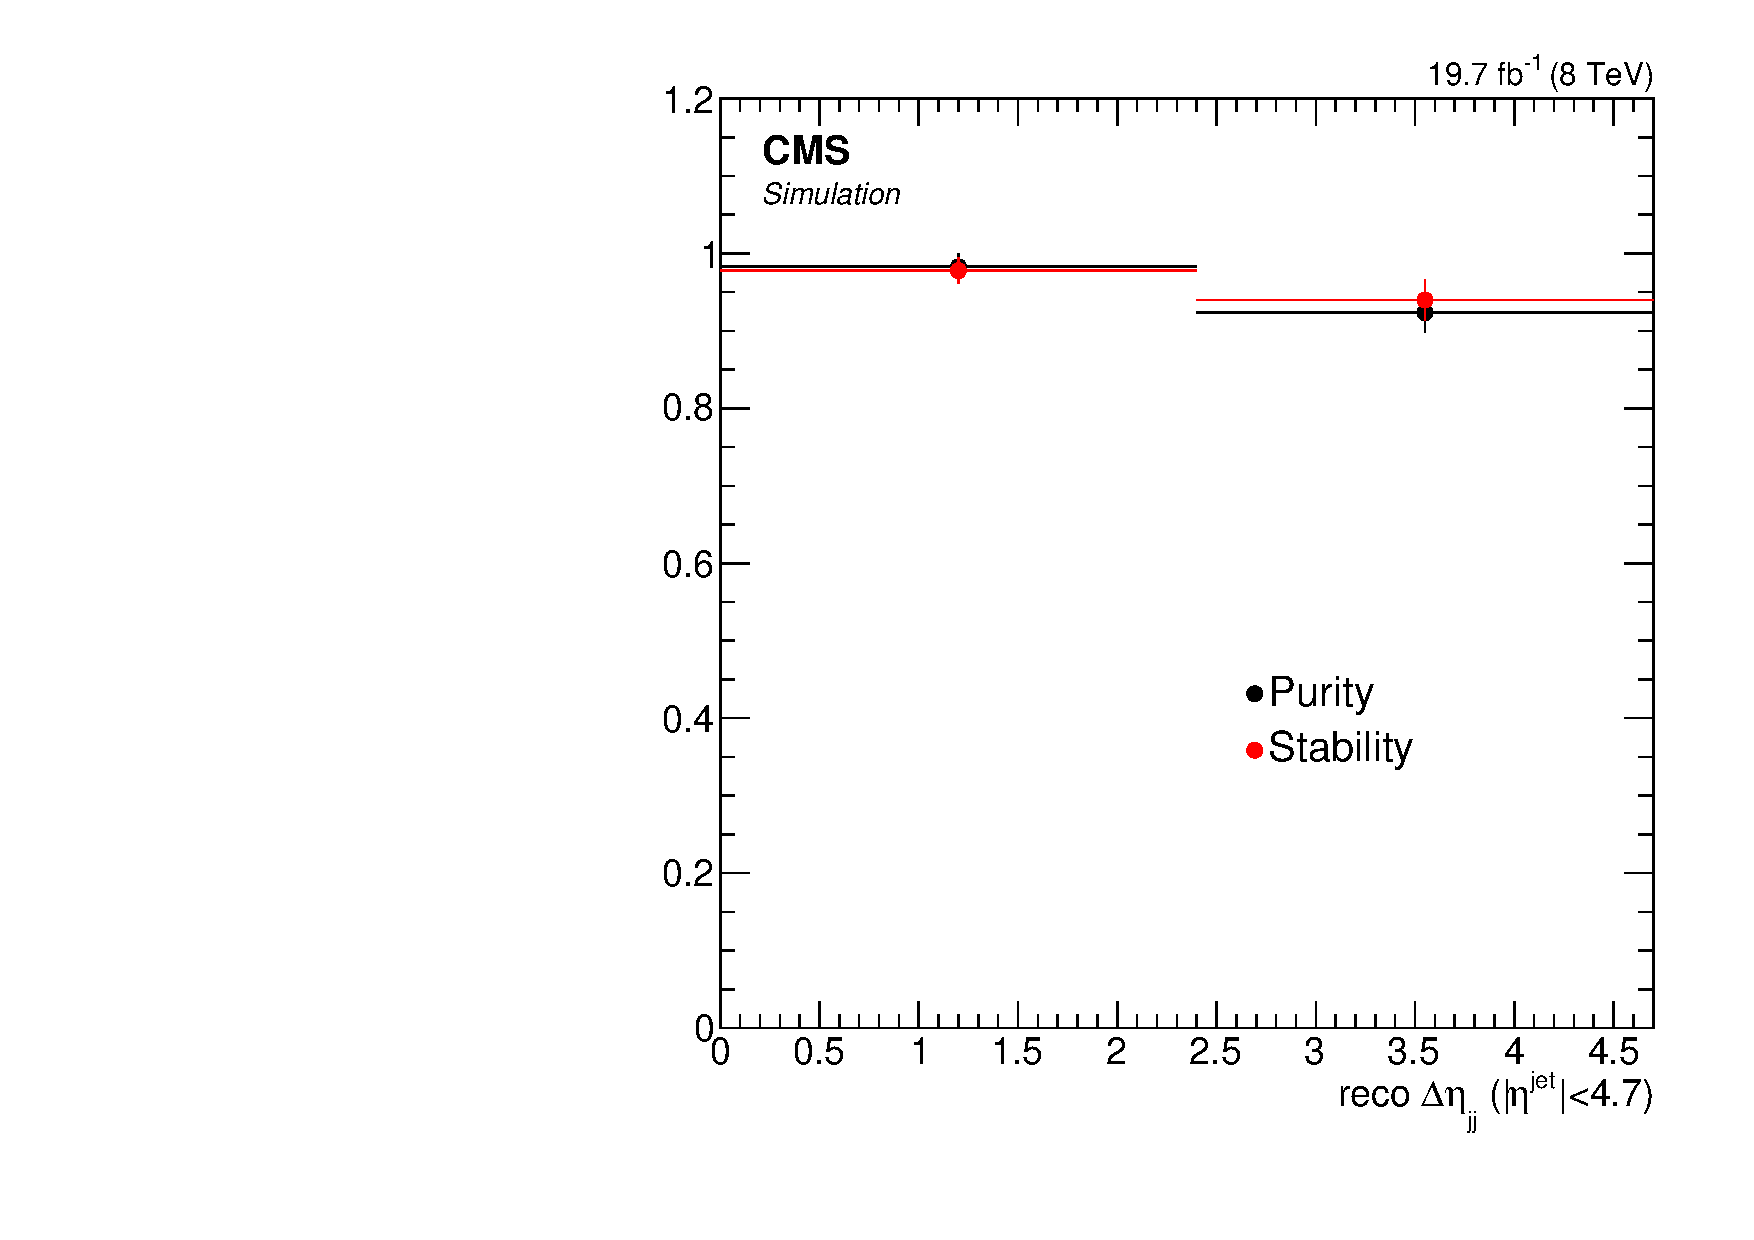
\includegraphics[width=0.8\cmsFigWidth]{Figures/Unfolding/BinMigration/PurityStability_4m_Deta_Mad}
    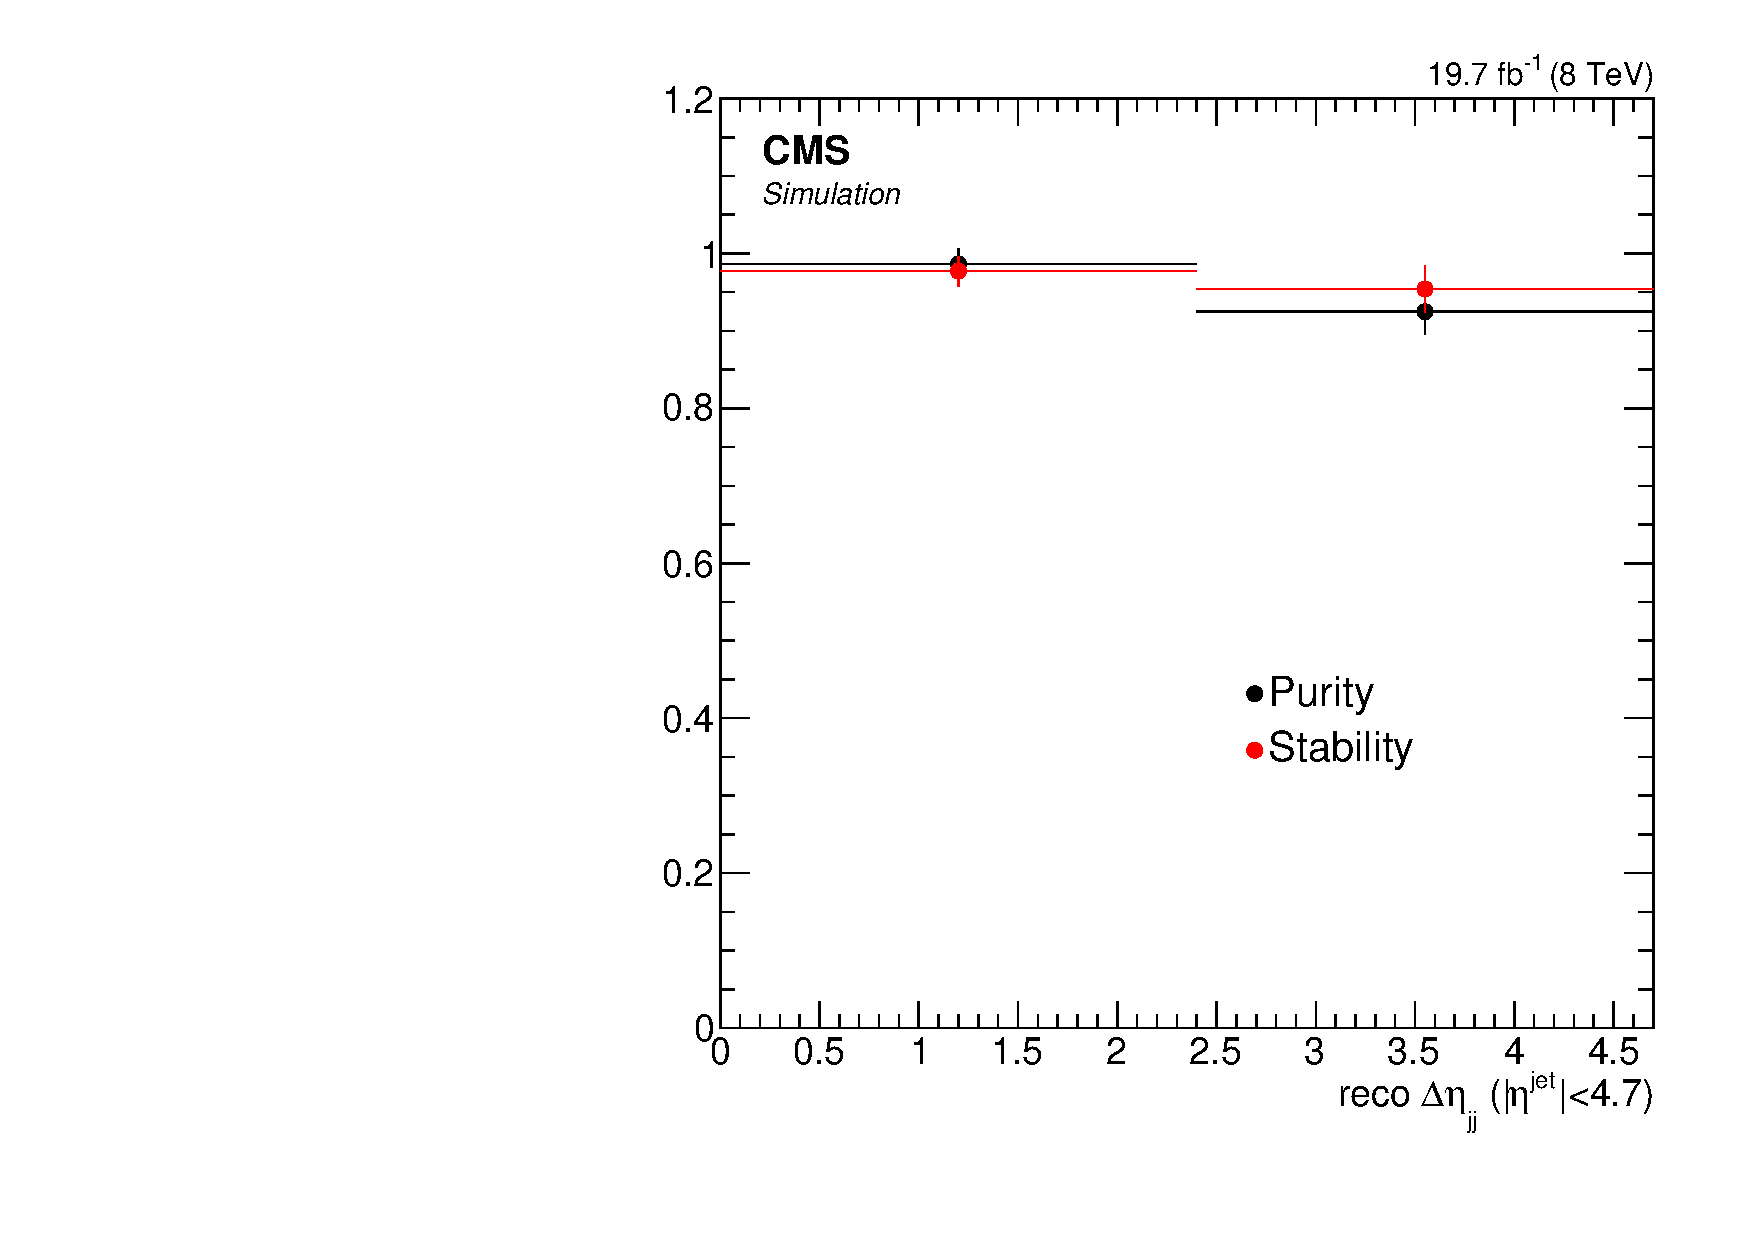
\includegraphics[width=0.8\cmsFigWidth]{Figures/Unfolding/BinMigration/PurityStability_4e_Deta_Mad}
    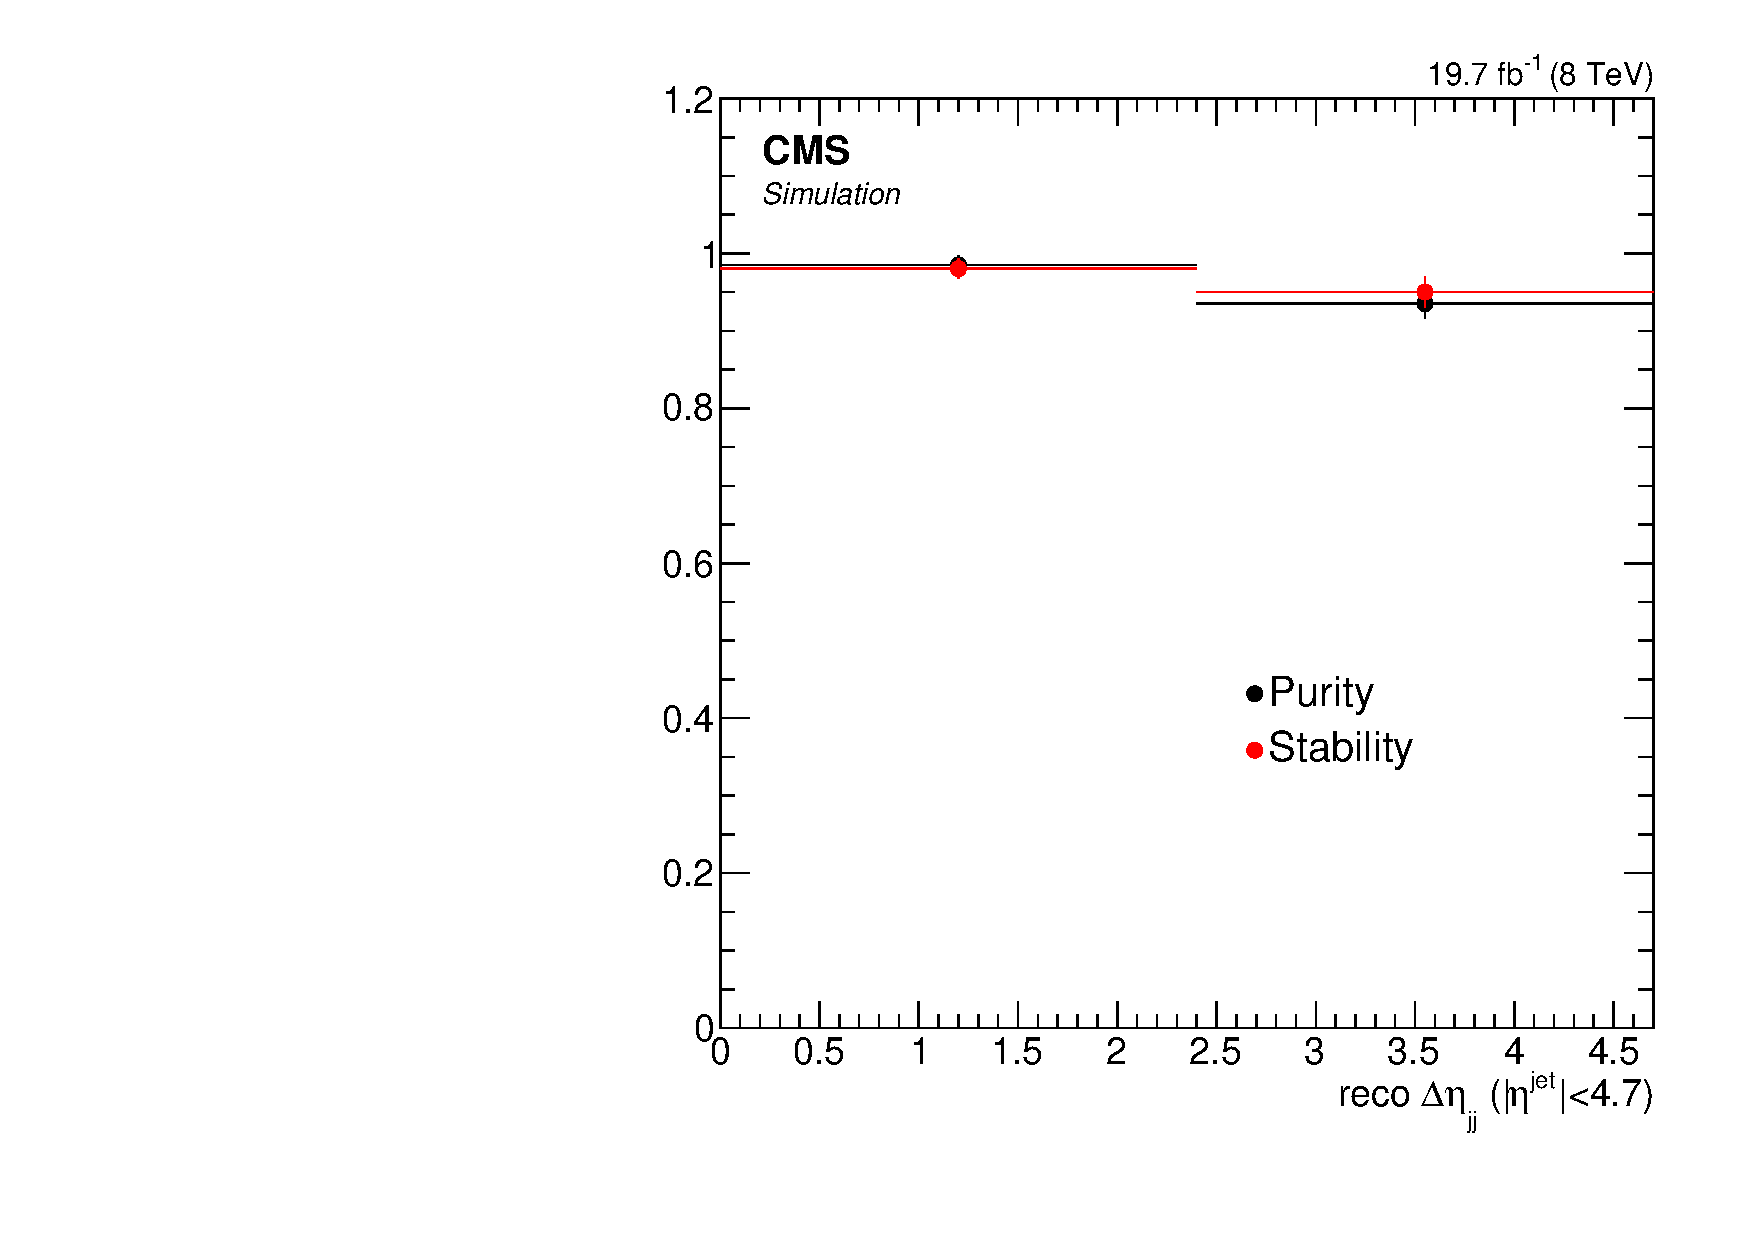
\includegraphics[width=0.8\cmsFigWidth]{Figures/Unfolding/BinMigration/PurityStability_2e2m_Deta_Mad}
    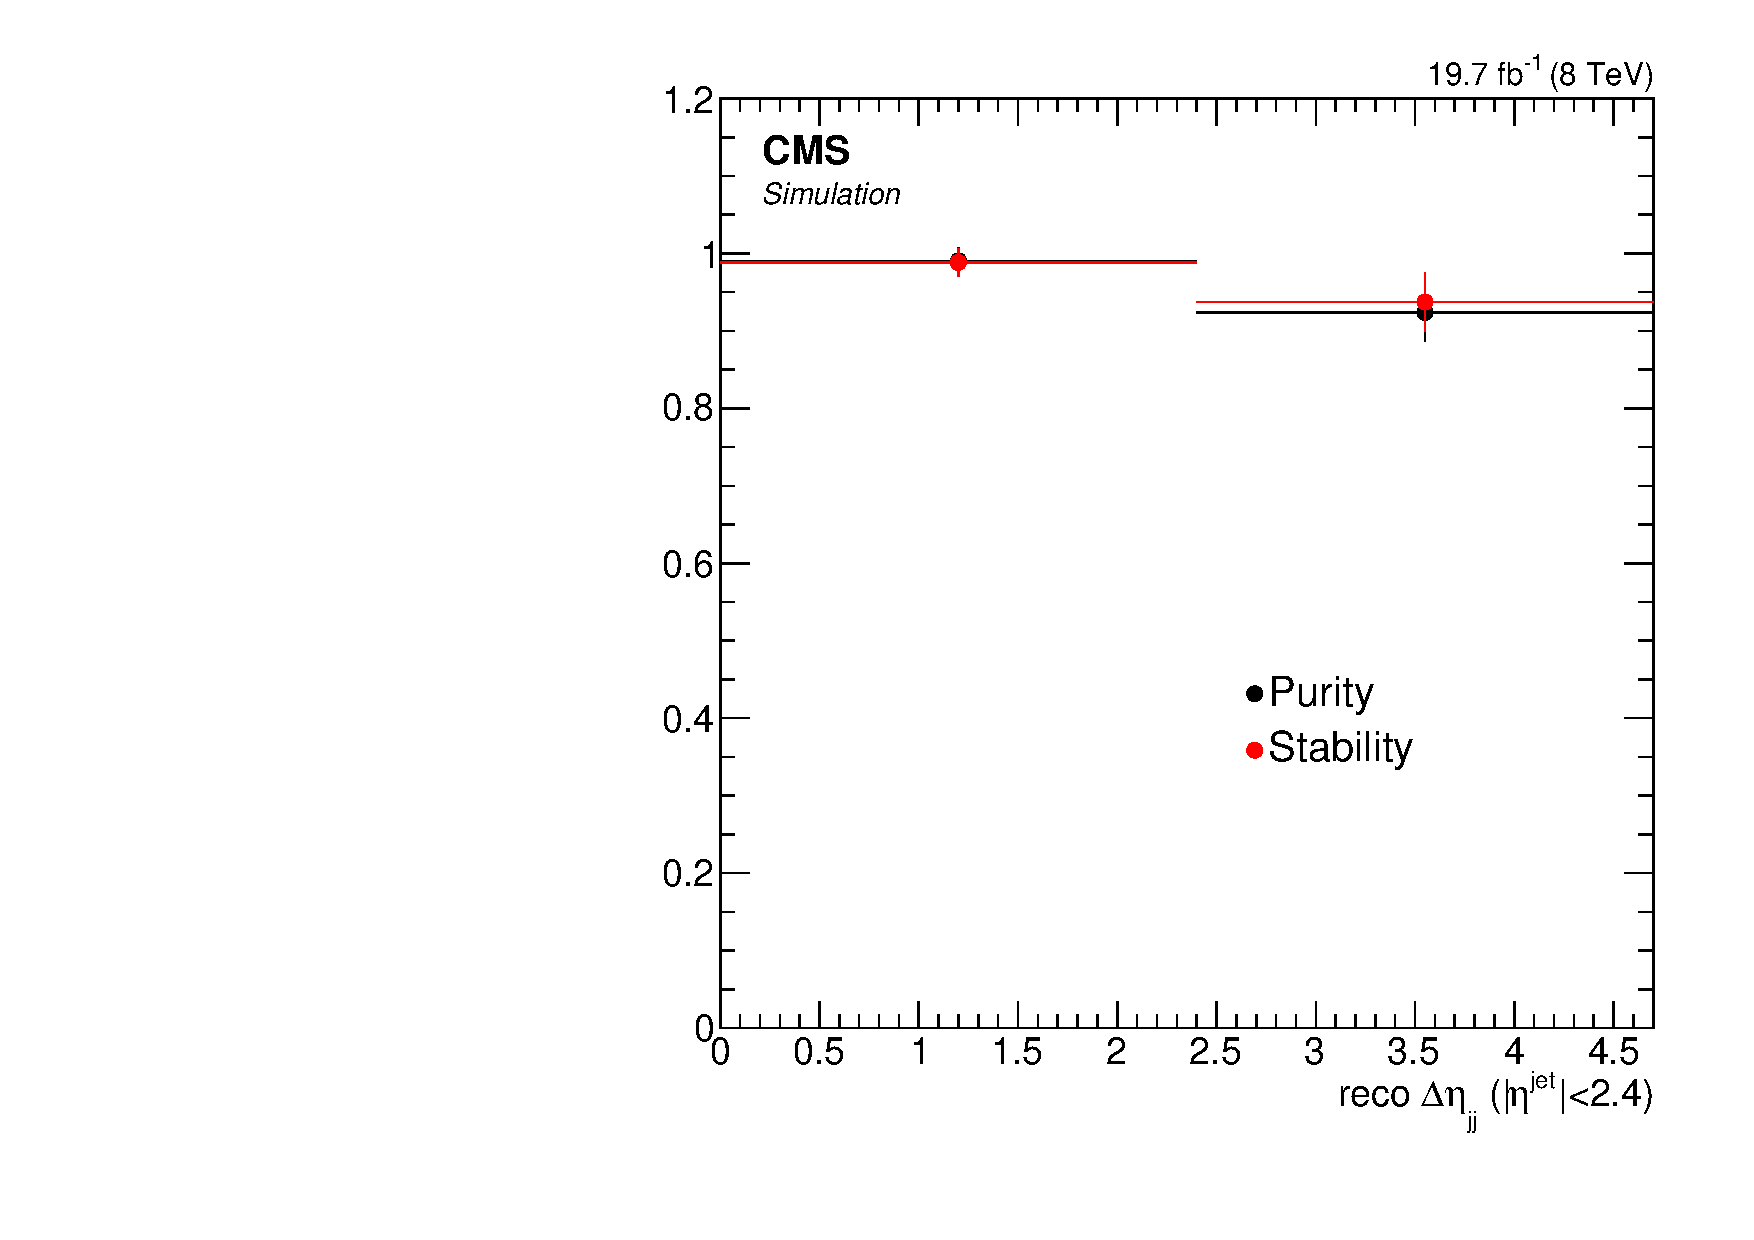
\includegraphics[width=0.8\cmsFigWidth]{Figures/Unfolding/BinMigration/PurityStability_4m_CentralDeta_Mad}
    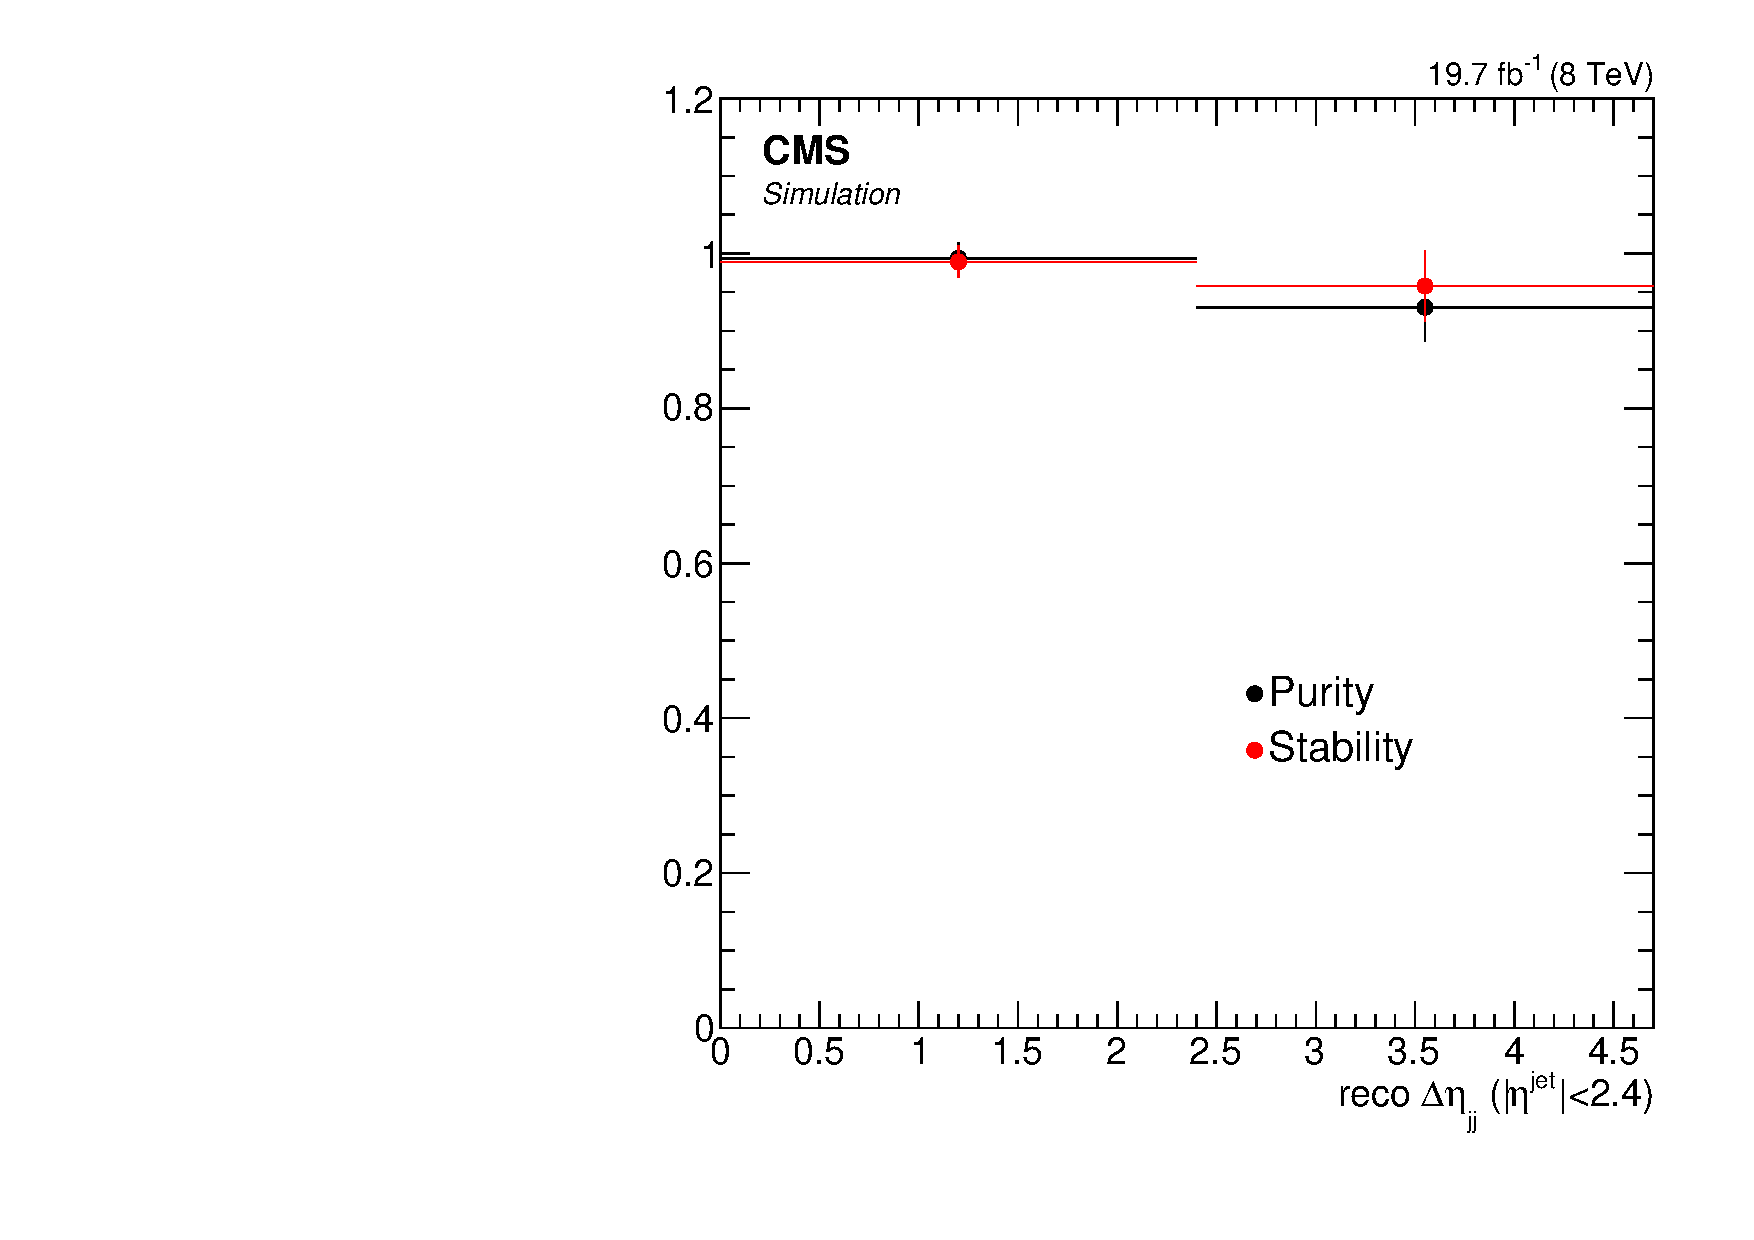
\includegraphics[width=0.8\cmsFigWidth]{Figures/Unfolding/BinMigration/PurityStability_4e_CentralDeta_Mad}
    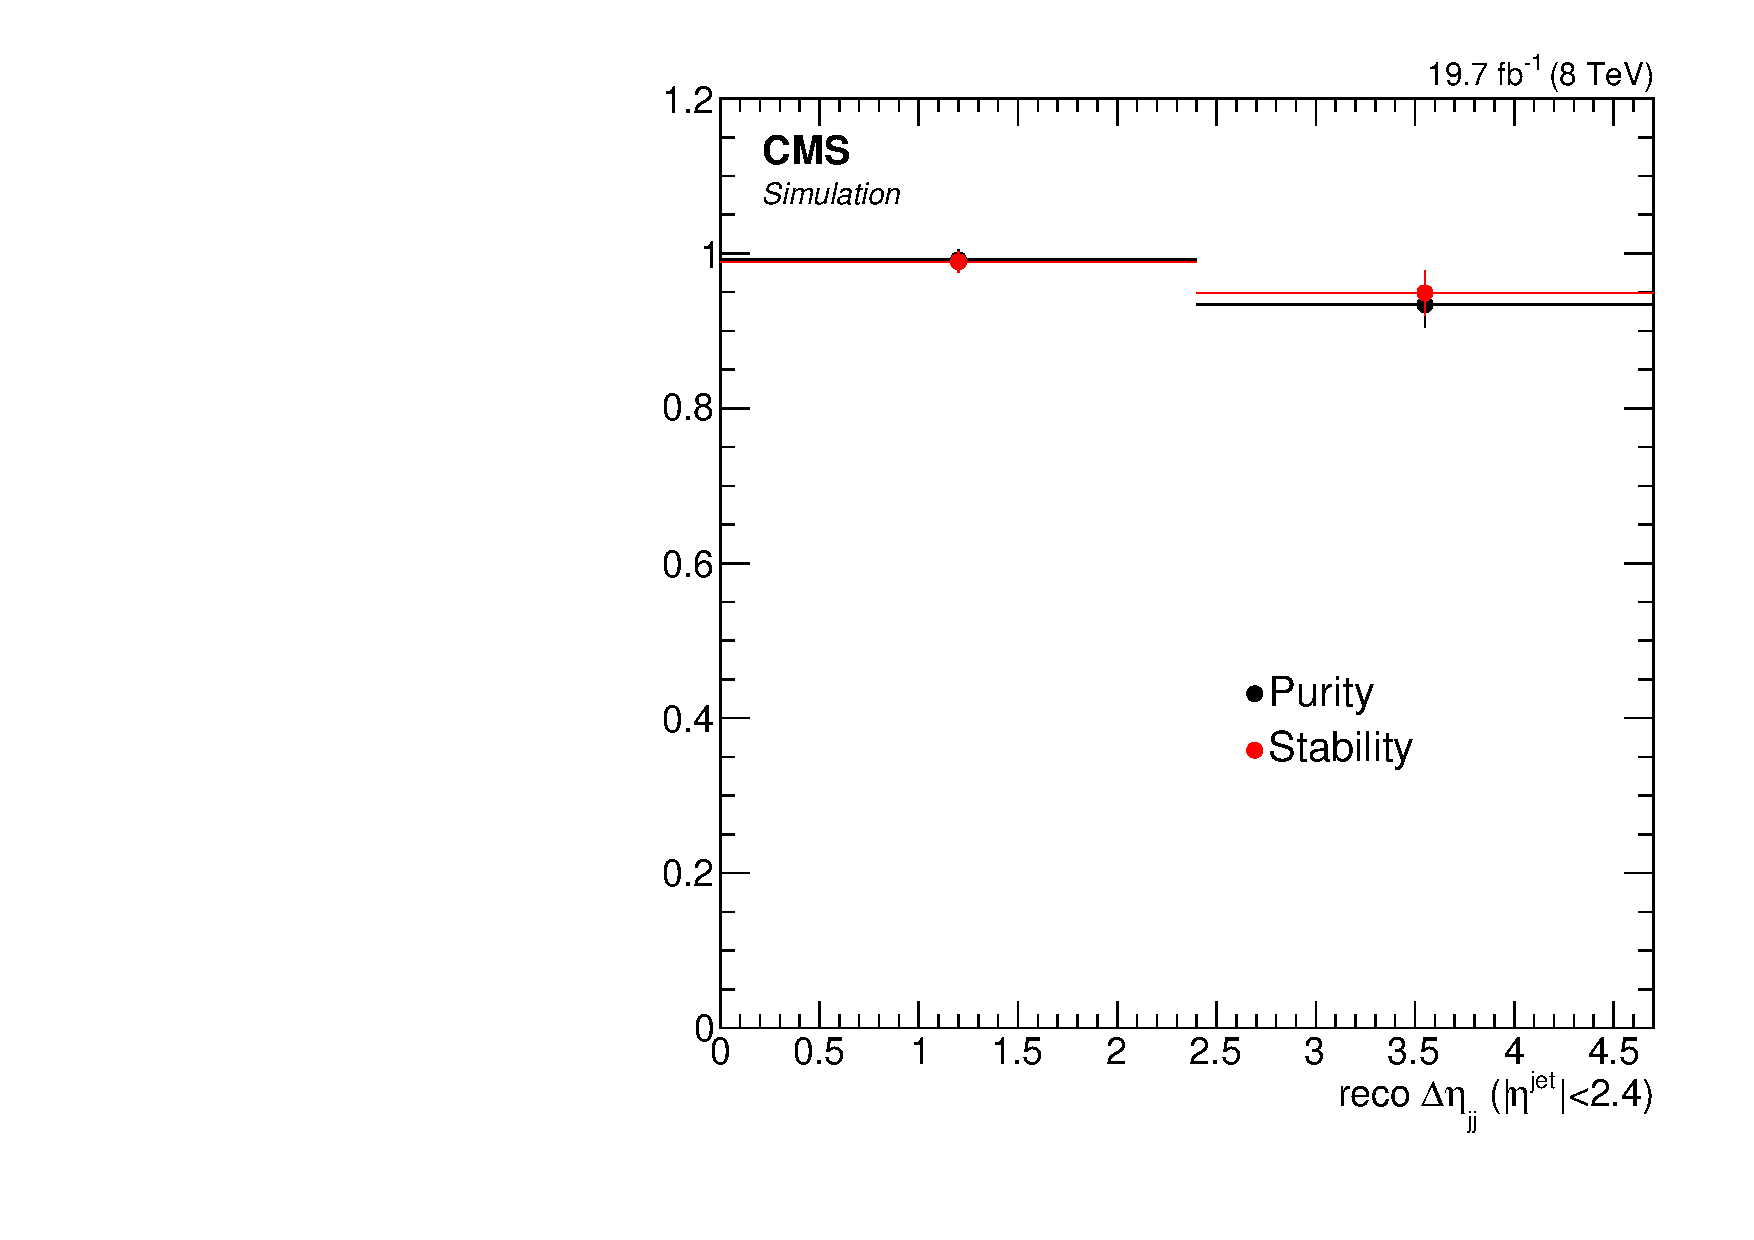
\includegraphics[width=0.8\cmsFigWidth]{Figures/Unfolding/BinMigration/PurityStability_2e2m_CentralDeta_Mad}
 \caption{Purity and stability as a function of the $\Delta\eta$ between the two most energetic jets (top) and  central jets (bottom) in the event,  for the $4\mu$ (left), $4e$ (center) and $2e2\mu$ (right) final states.}
    \label{fig:ps_deta}
  \end{center}
\end{figure}

\begin{figure}[hbtp]
  \begin{center}
    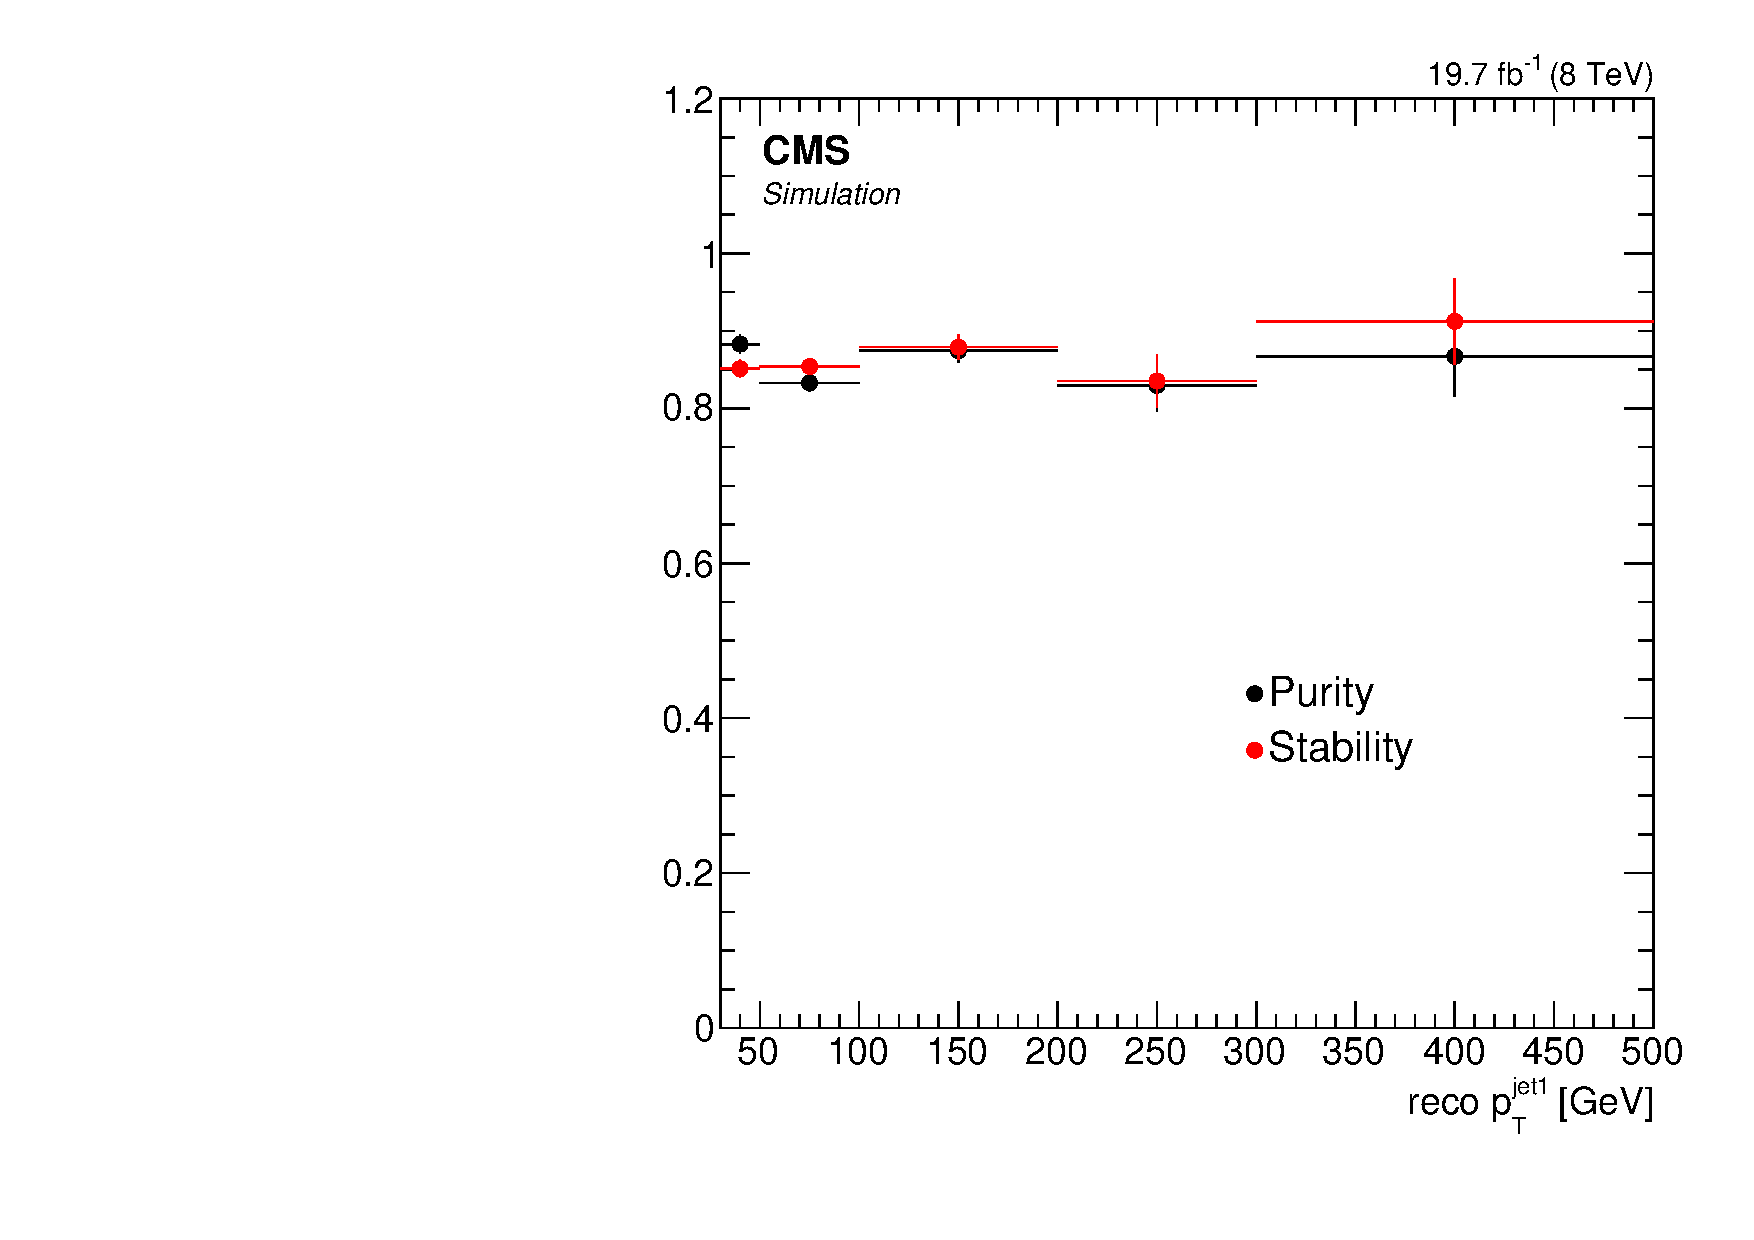
\includegraphics[width=0.8\cmsFigWidth]{Figures/Unfolding/BinMigration/PurityStability_4m_PtJet1_Mad}
    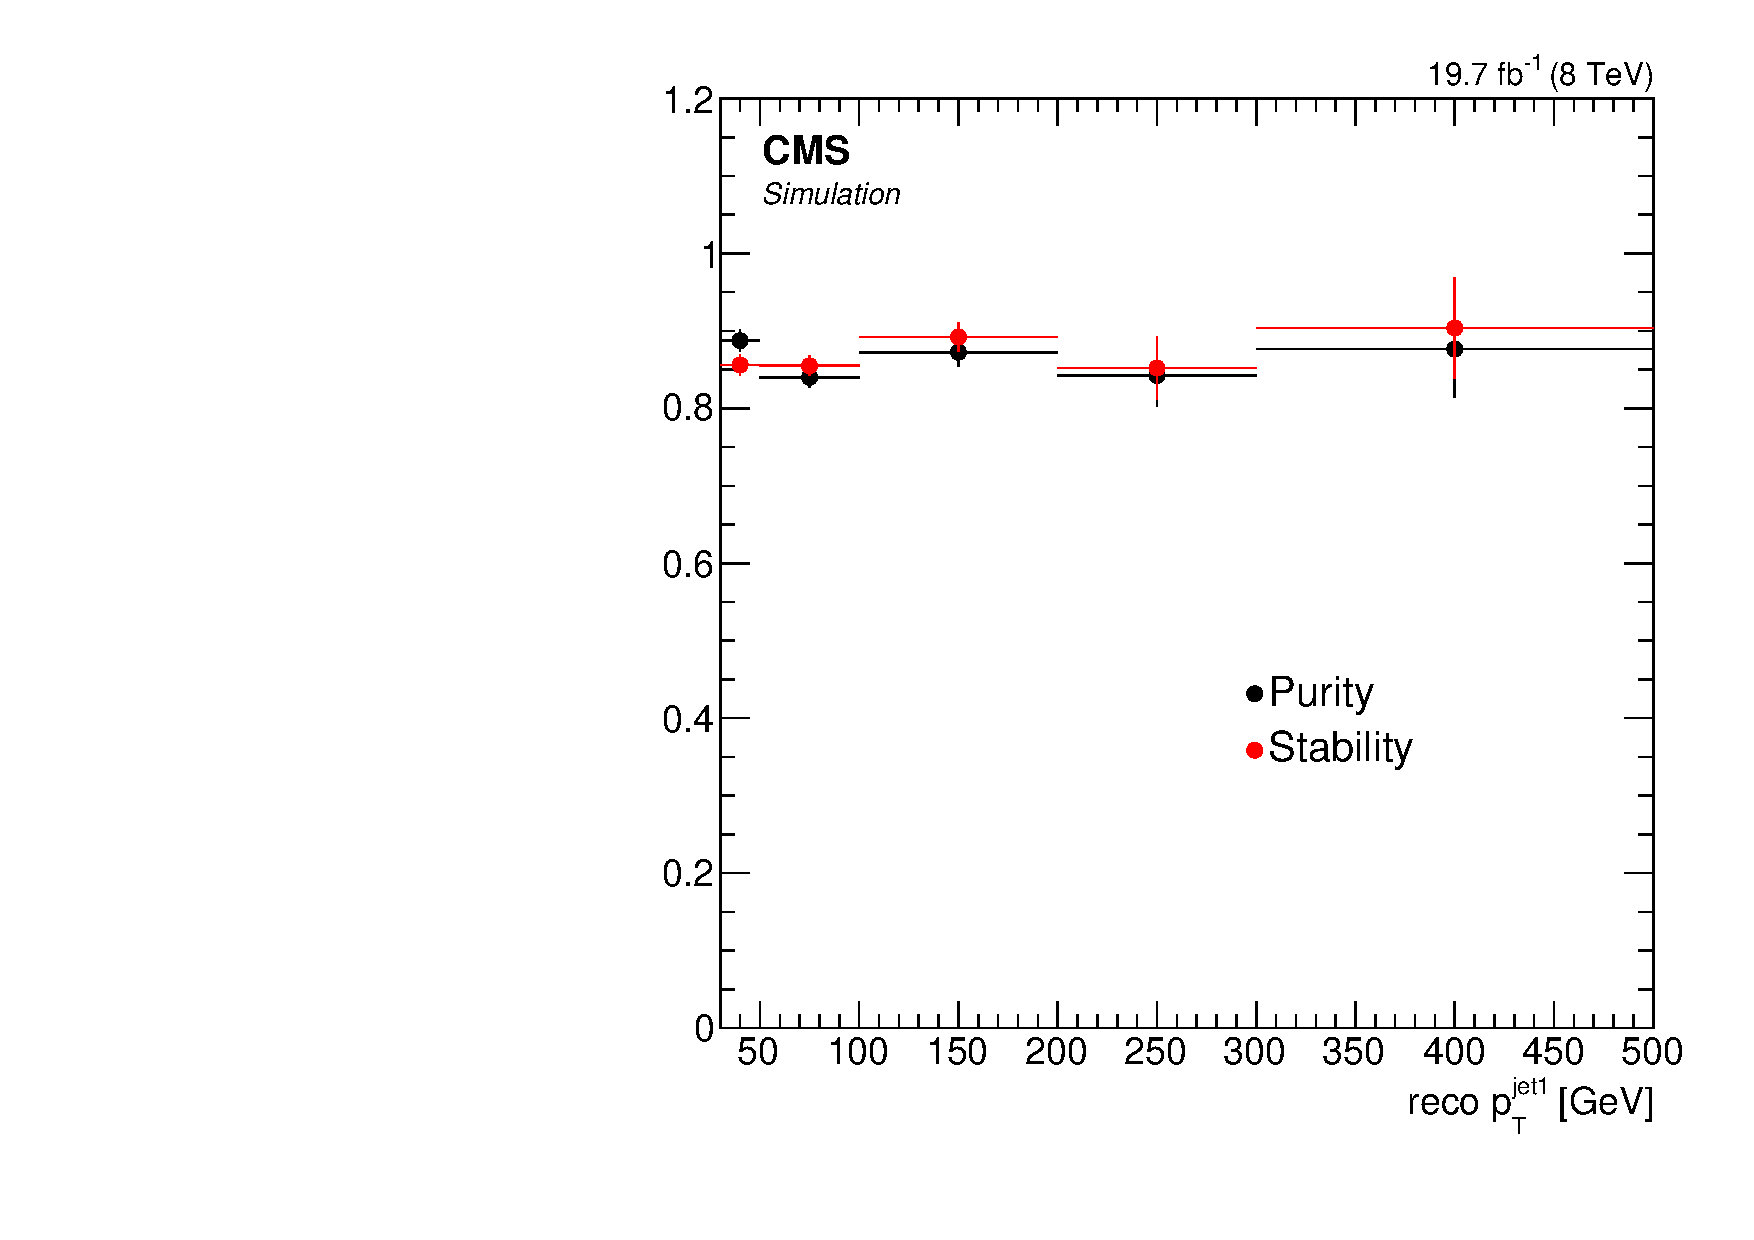
\includegraphics[width=0.8\cmsFigWidth]{Figures/Unfolding/BinMigration/PurityStability_4e_PtJet1_Mad}
    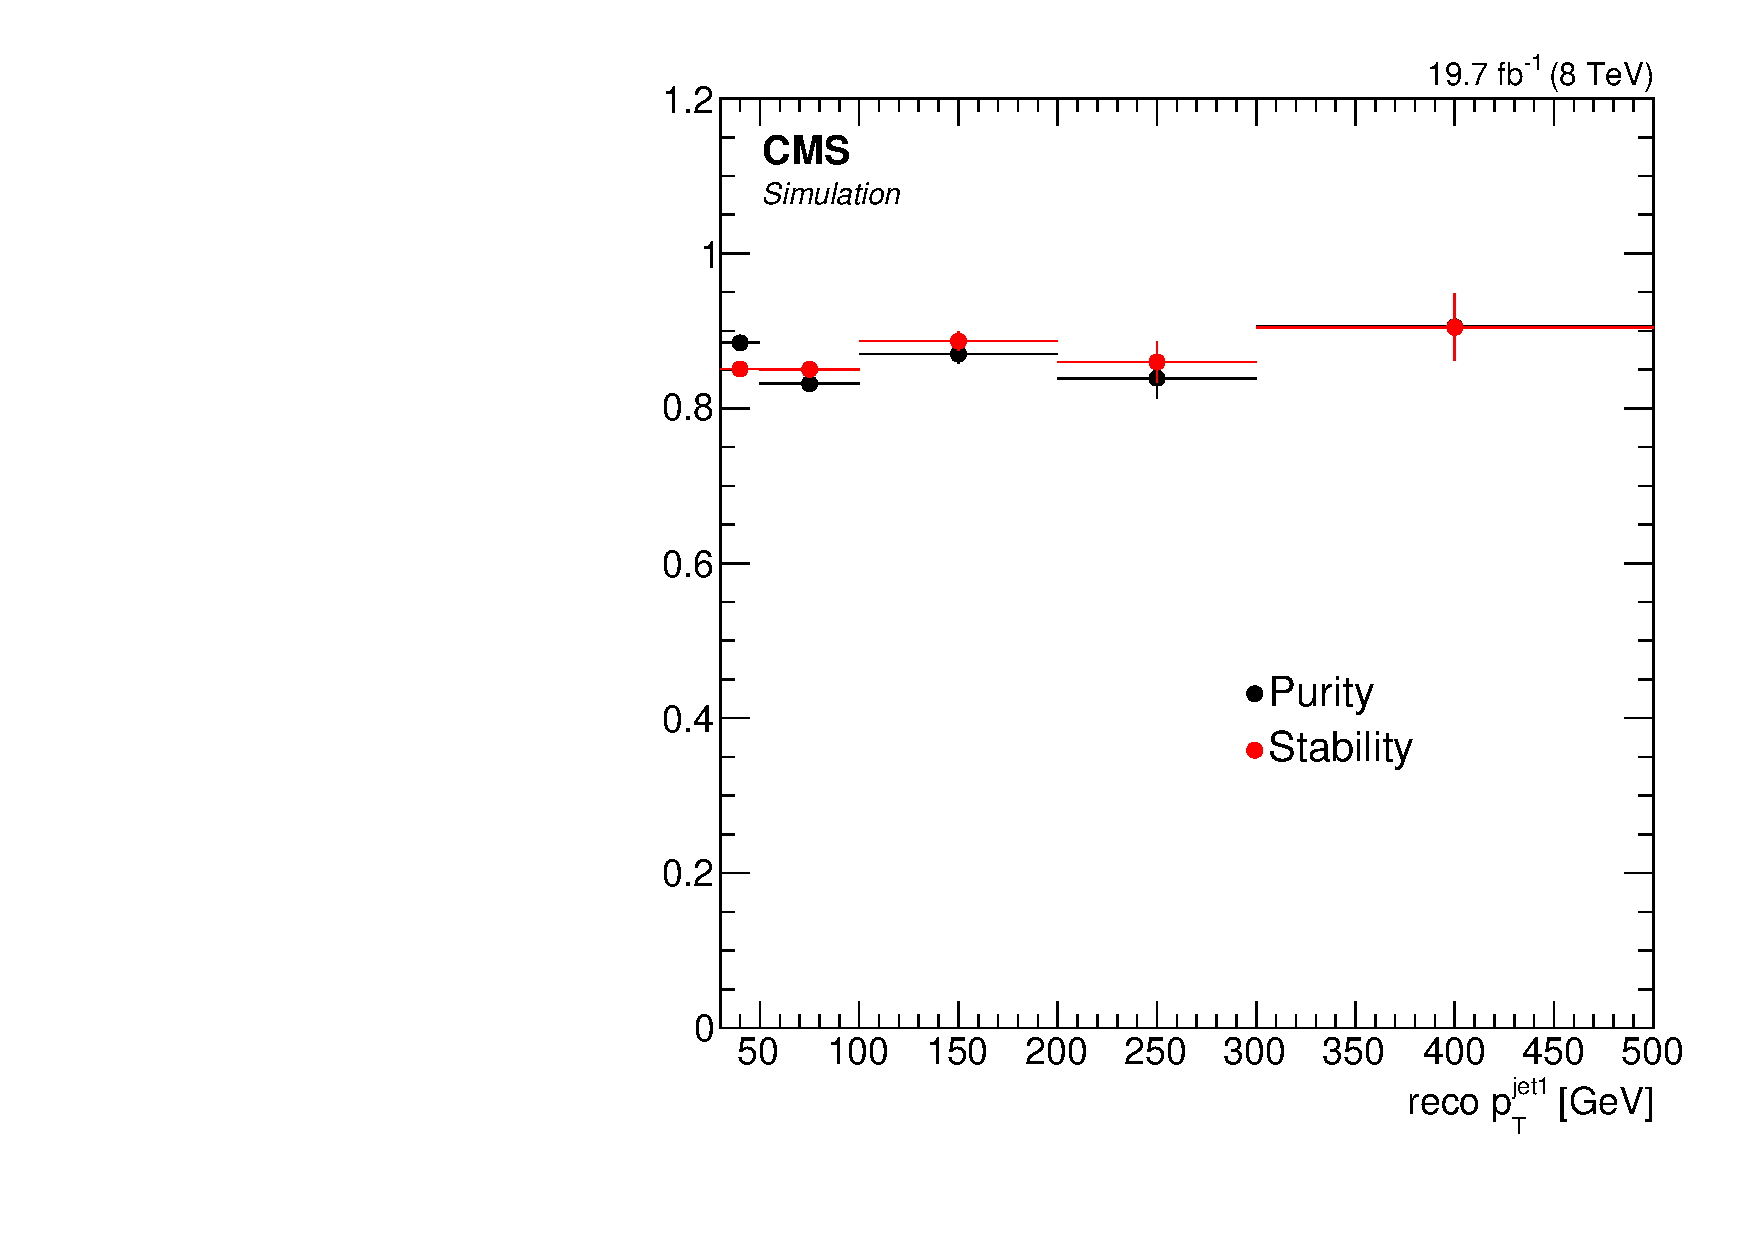
\includegraphics[width=0.8\cmsFigWidth]{Figures/Unfolding/BinMigration/PurityStability_2e2m_PtJet1_Mad}
    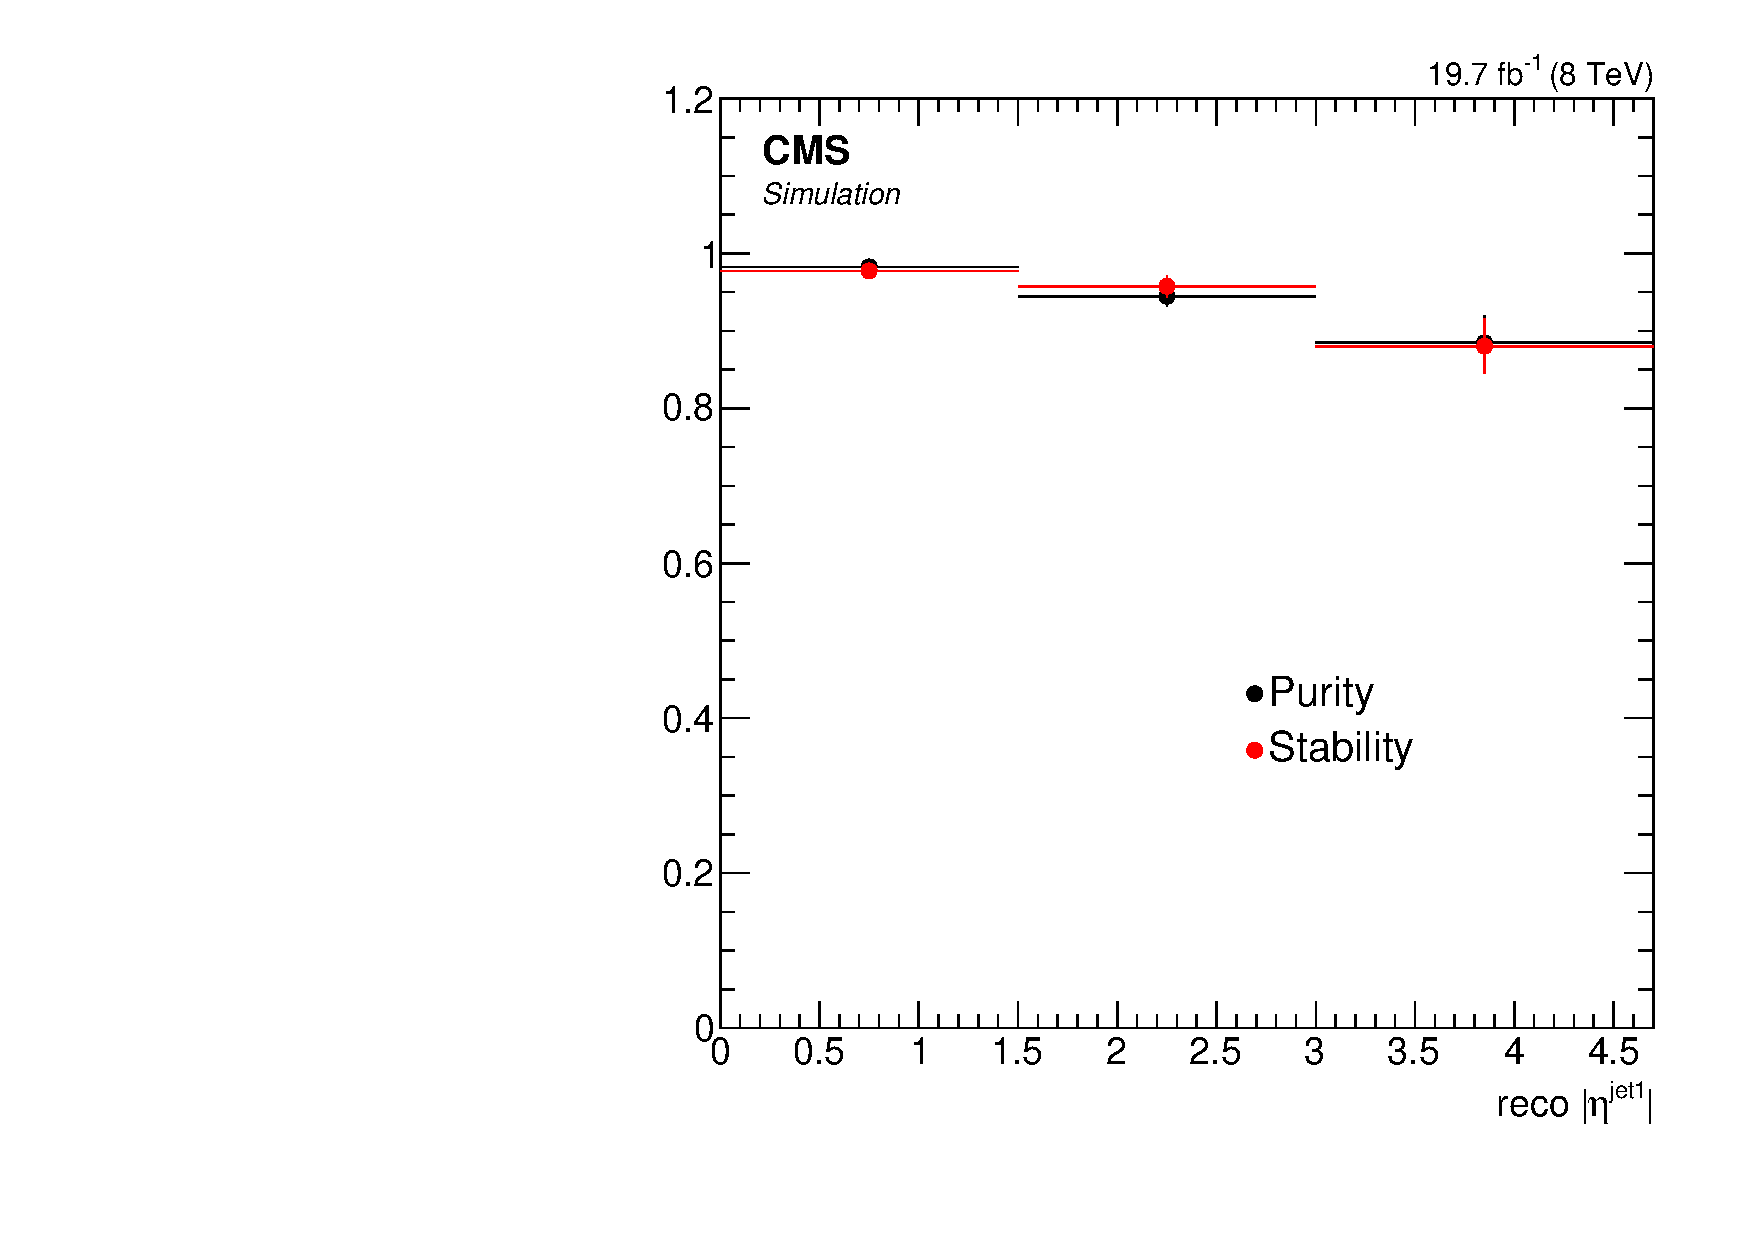
\includegraphics[width=0.8\cmsFigWidth]{Figures/Unfolding/BinMigration/PurityStability_4m_EtaJet1_Mad}
    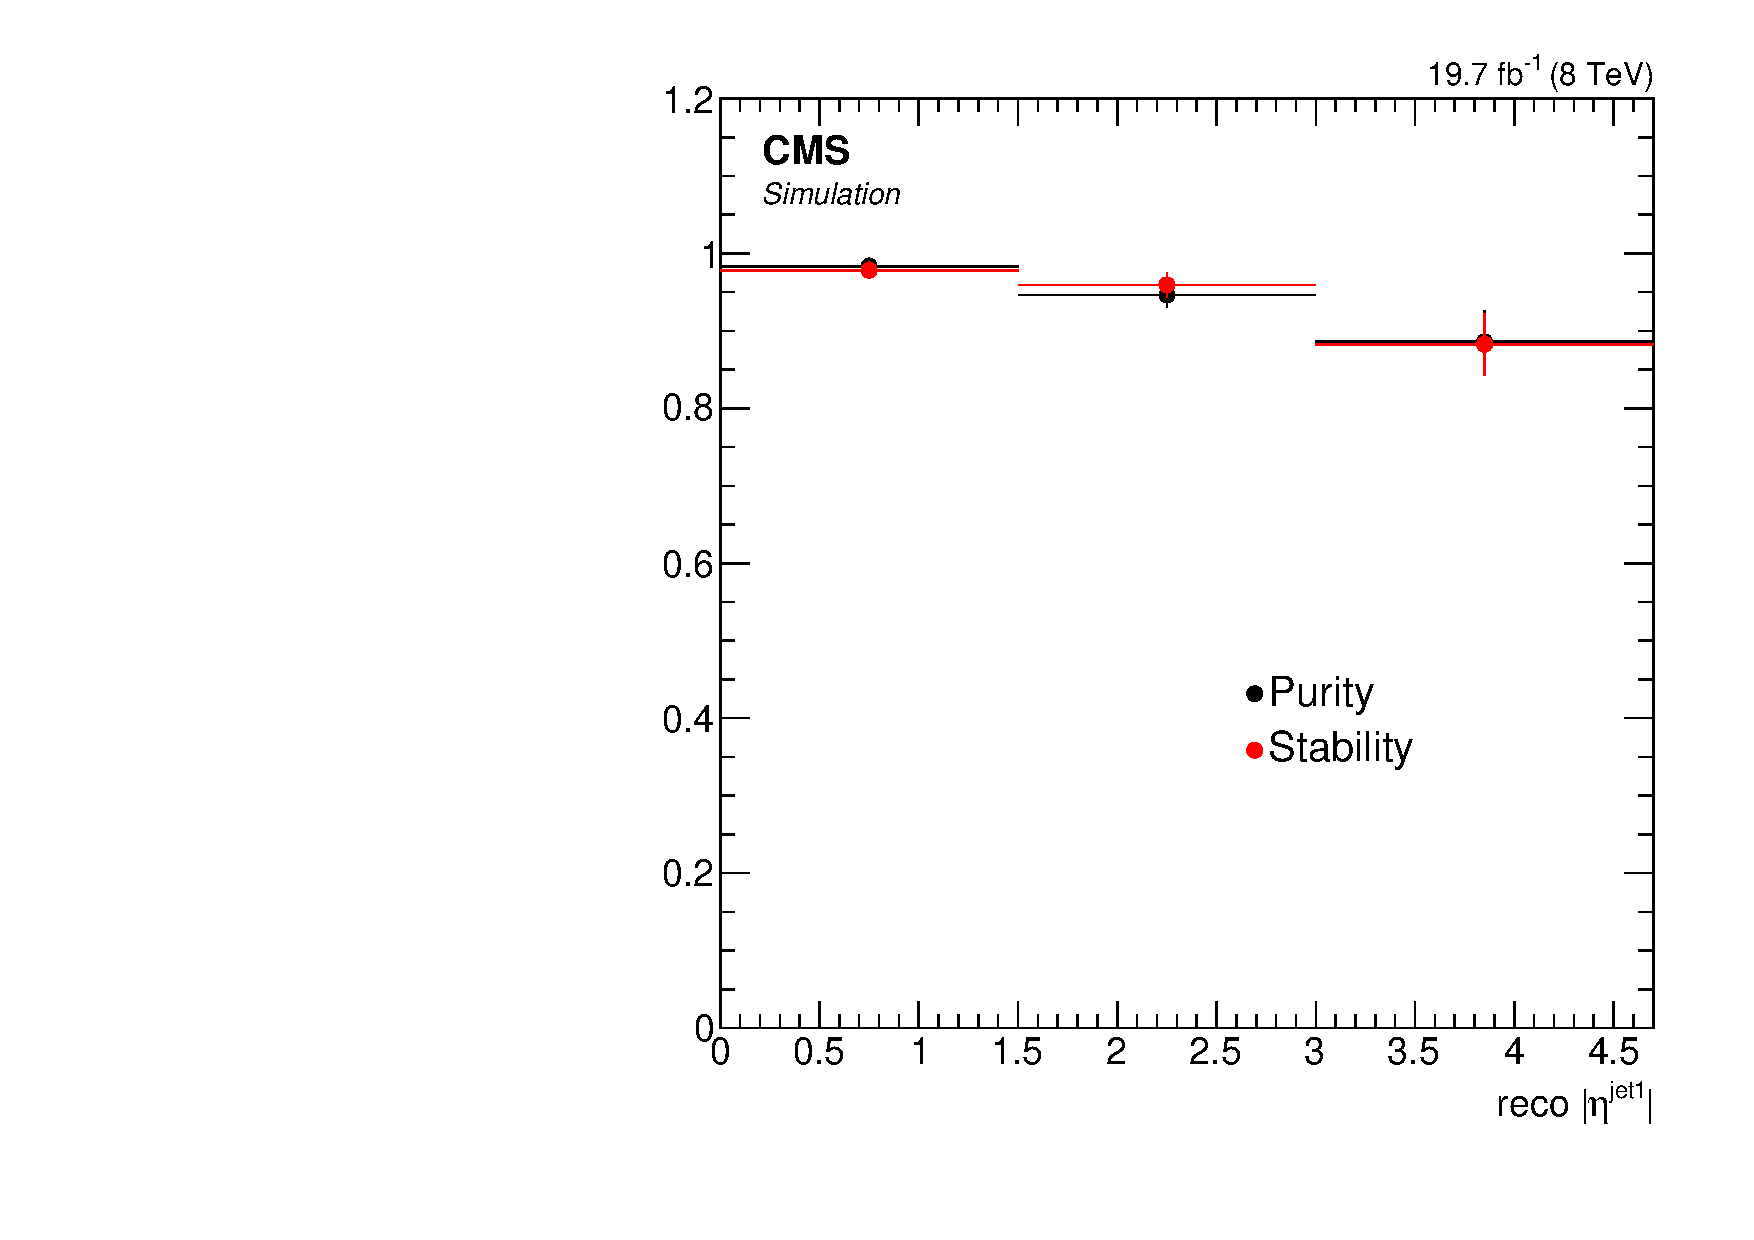
\includegraphics[width=0.8\cmsFigWidth]{Figures/Unfolding/BinMigration/PurityStability_4e_EtaJet1_Mad}
    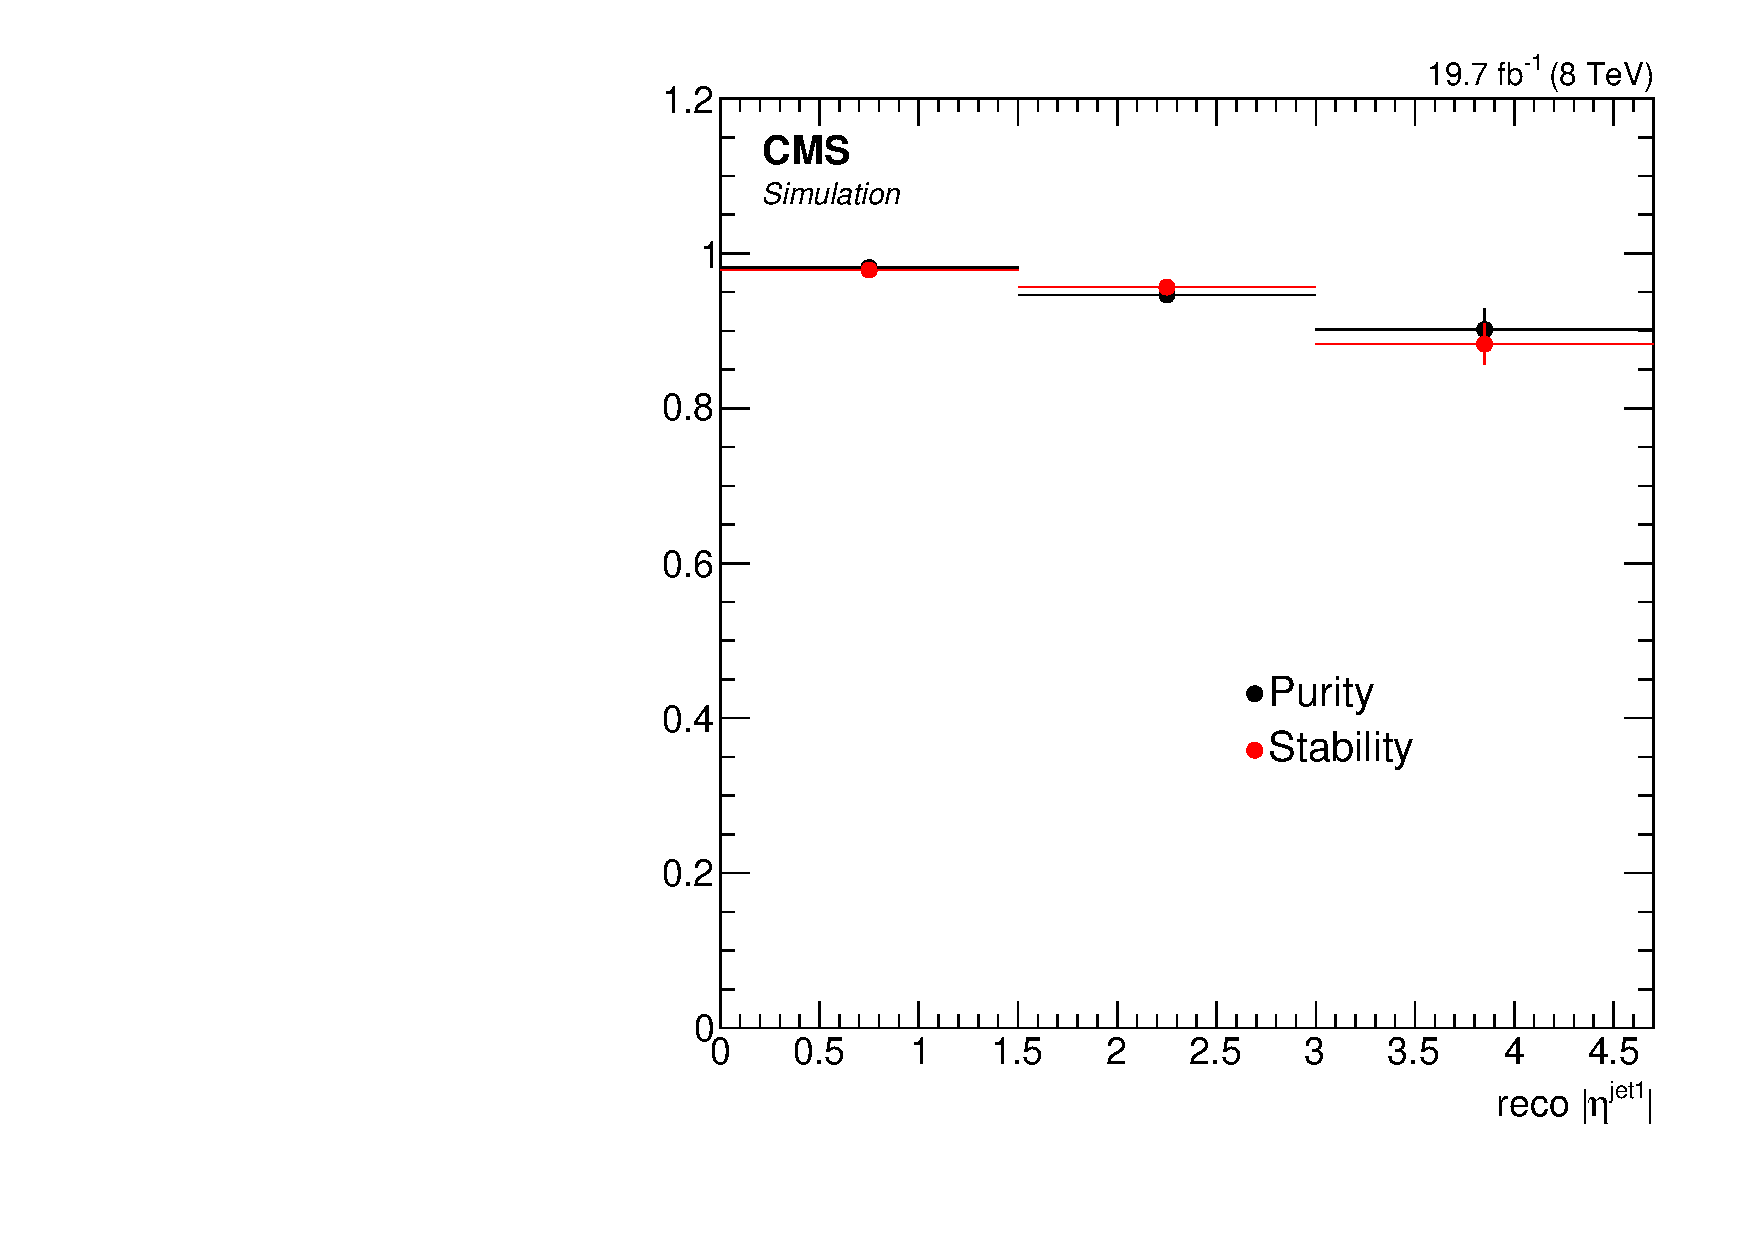
\includegraphics[width=0.8\cmsFigWidth]{Figures/Unfolding/BinMigration/PurityStability_2e2m_EtaJet1_Mad}
 \caption{Purity and stability as a function of the $p_T$ (top) and $\eta$ (bottom) of the most energetic jet in the event,  for the $4\mu$ (left), $4e$ (center) and $2e2\mu$ (right) final states.}
    \label{fig:ps_jet1}
  \end{center}
\end{figure}
\begin{figure}[hbtp]
  \begin{center}
    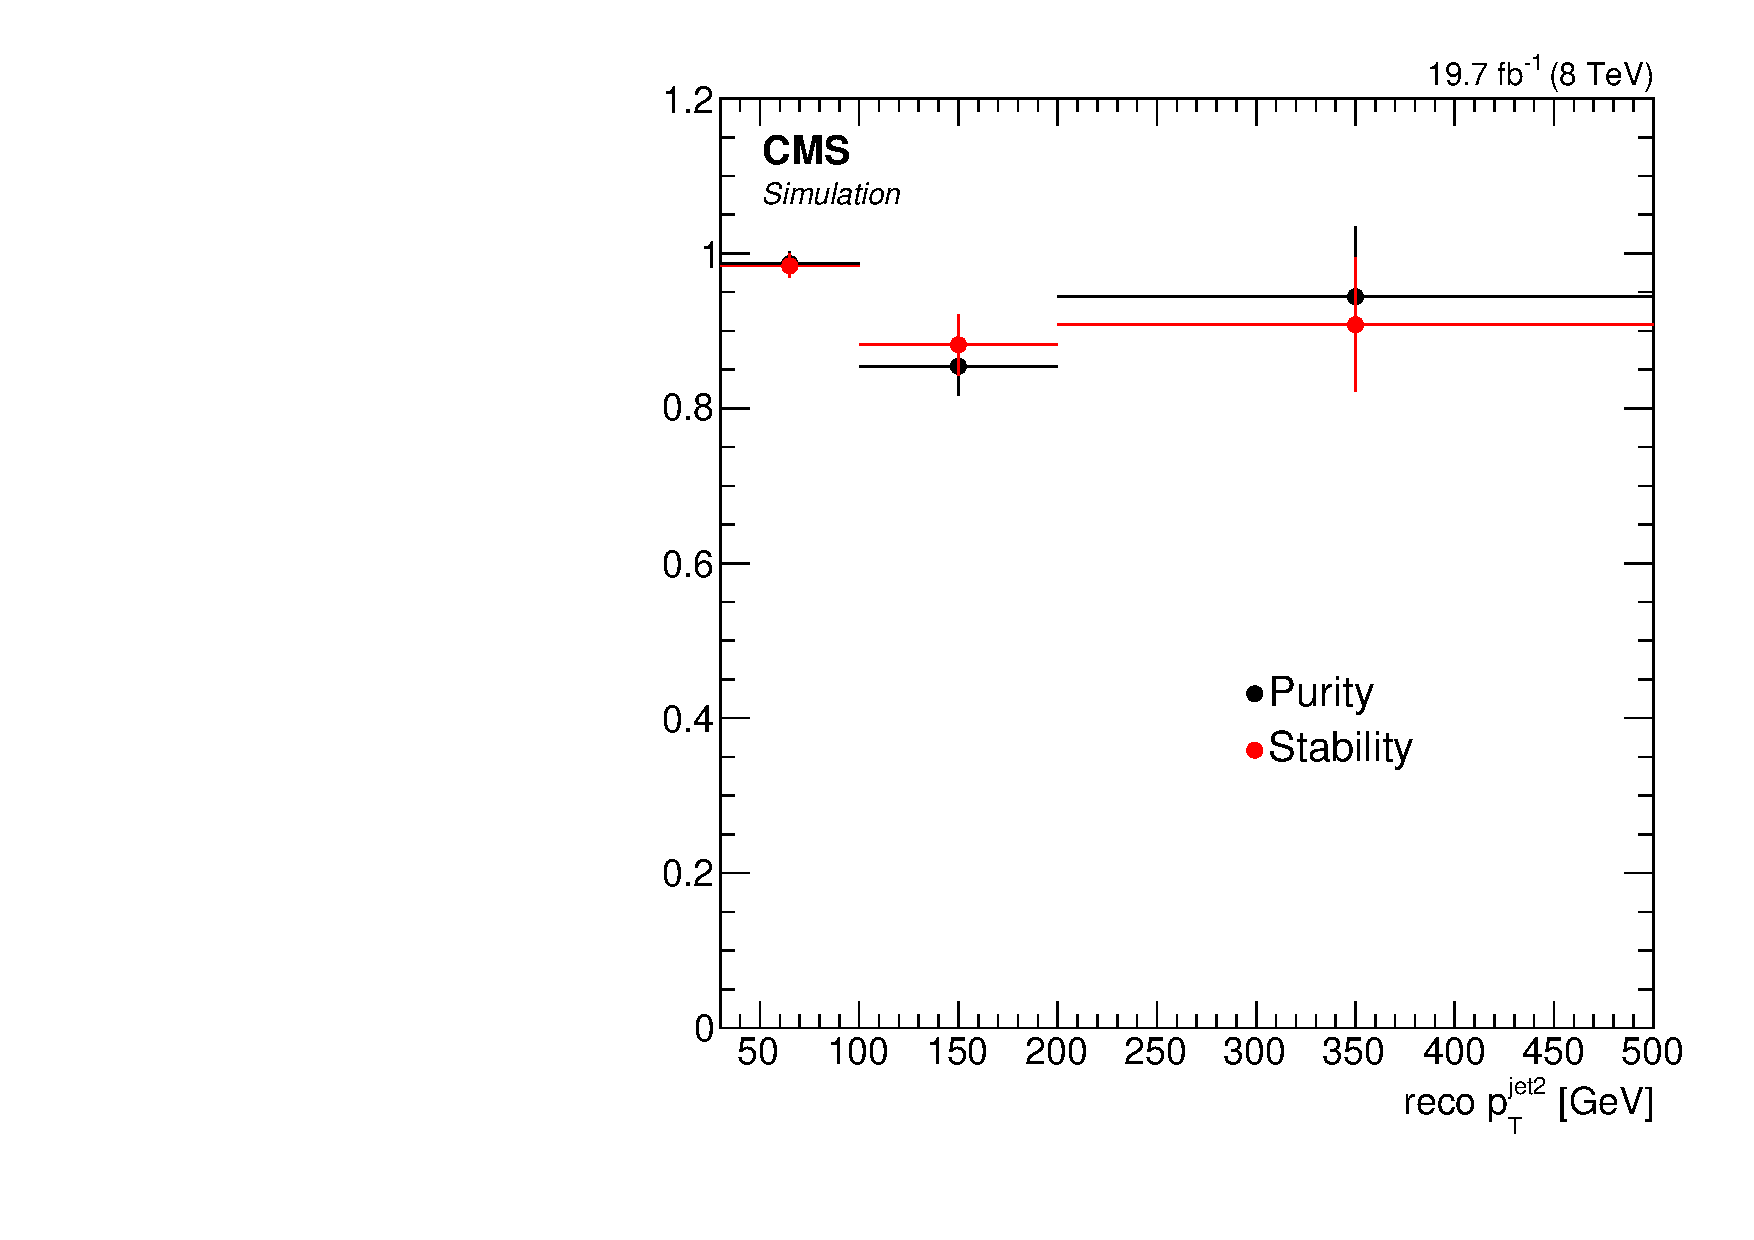
\includegraphics[width=0.8\cmsFigWidth]{Figures/Unfolding/BinMigration/PurityStability_4m_PtJet2_Mad}
    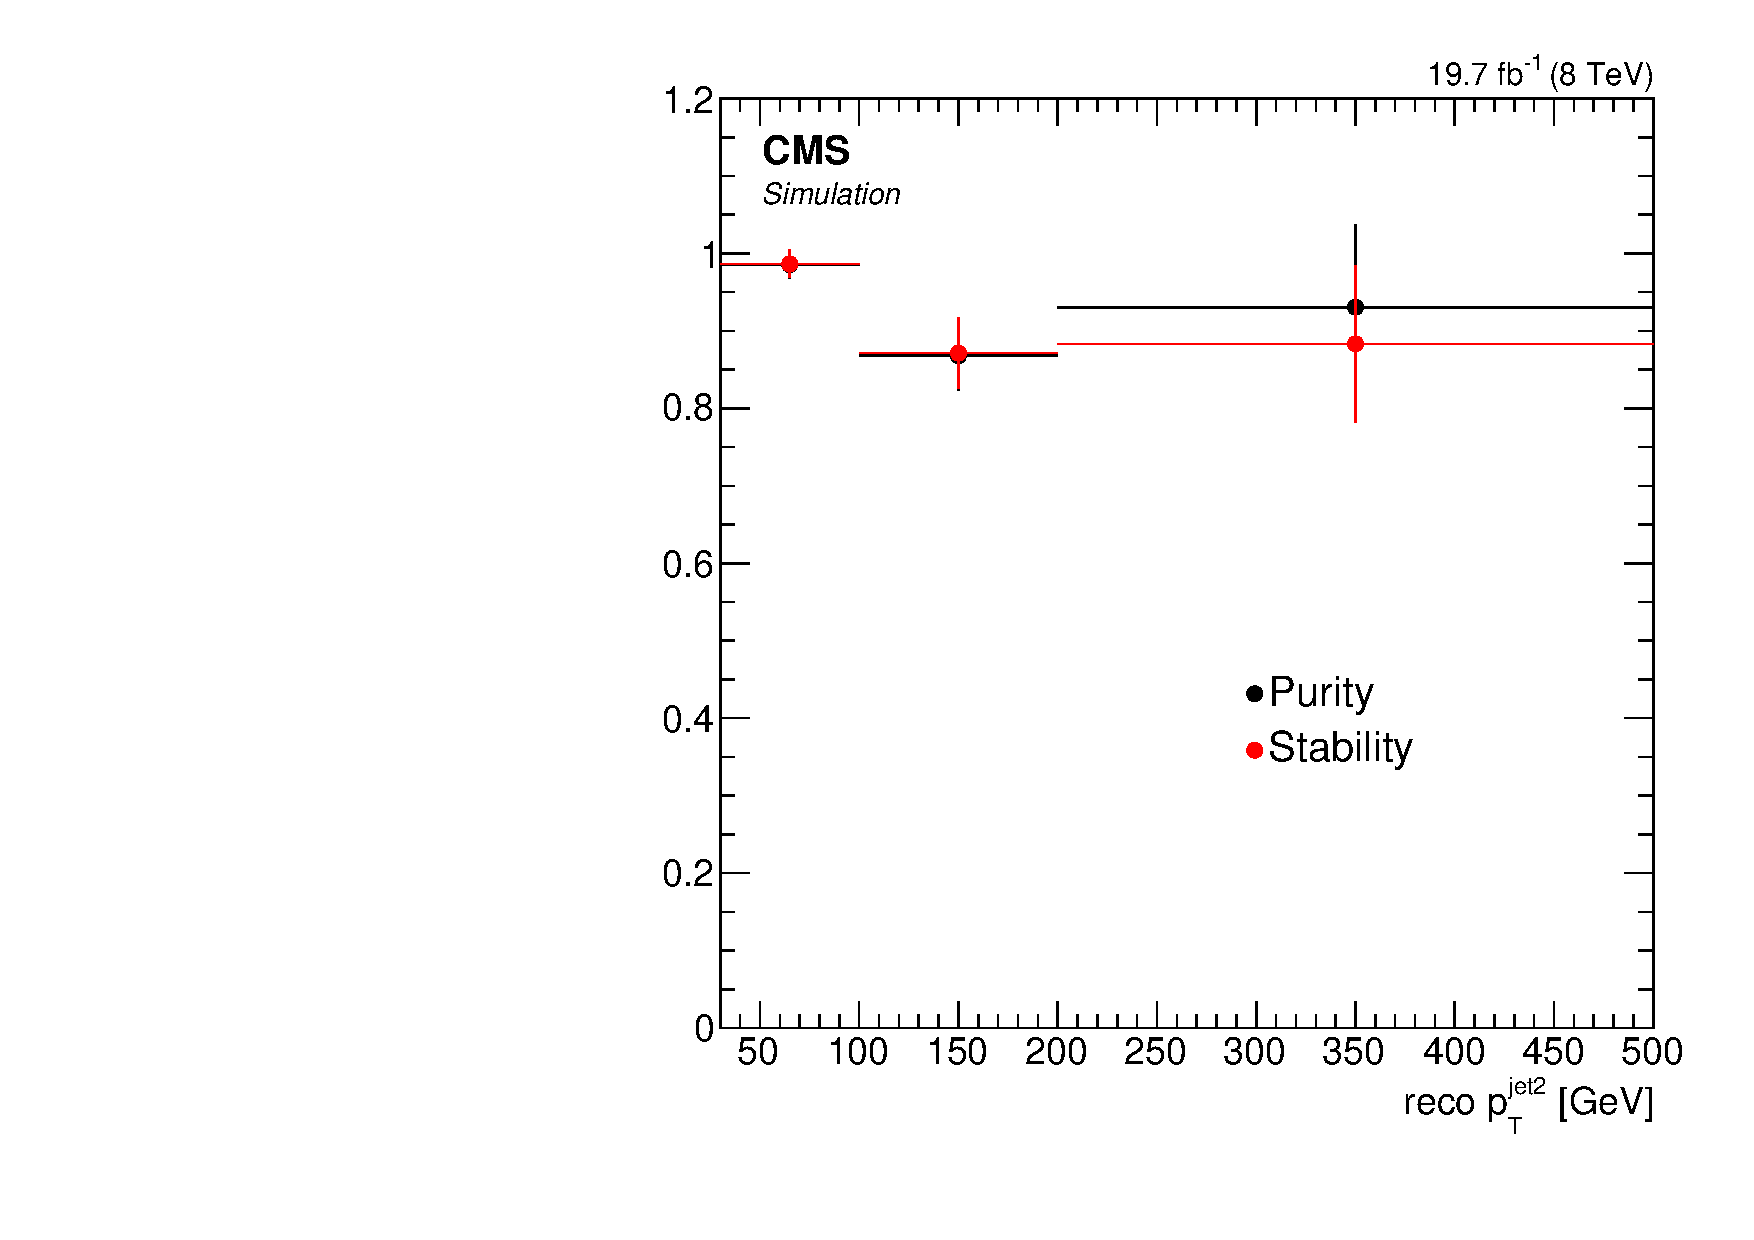
\includegraphics[width=0.8\cmsFigWidth]{Figures/Unfolding/BinMigration/PurityStability_4e_PtJet2_Mad}
    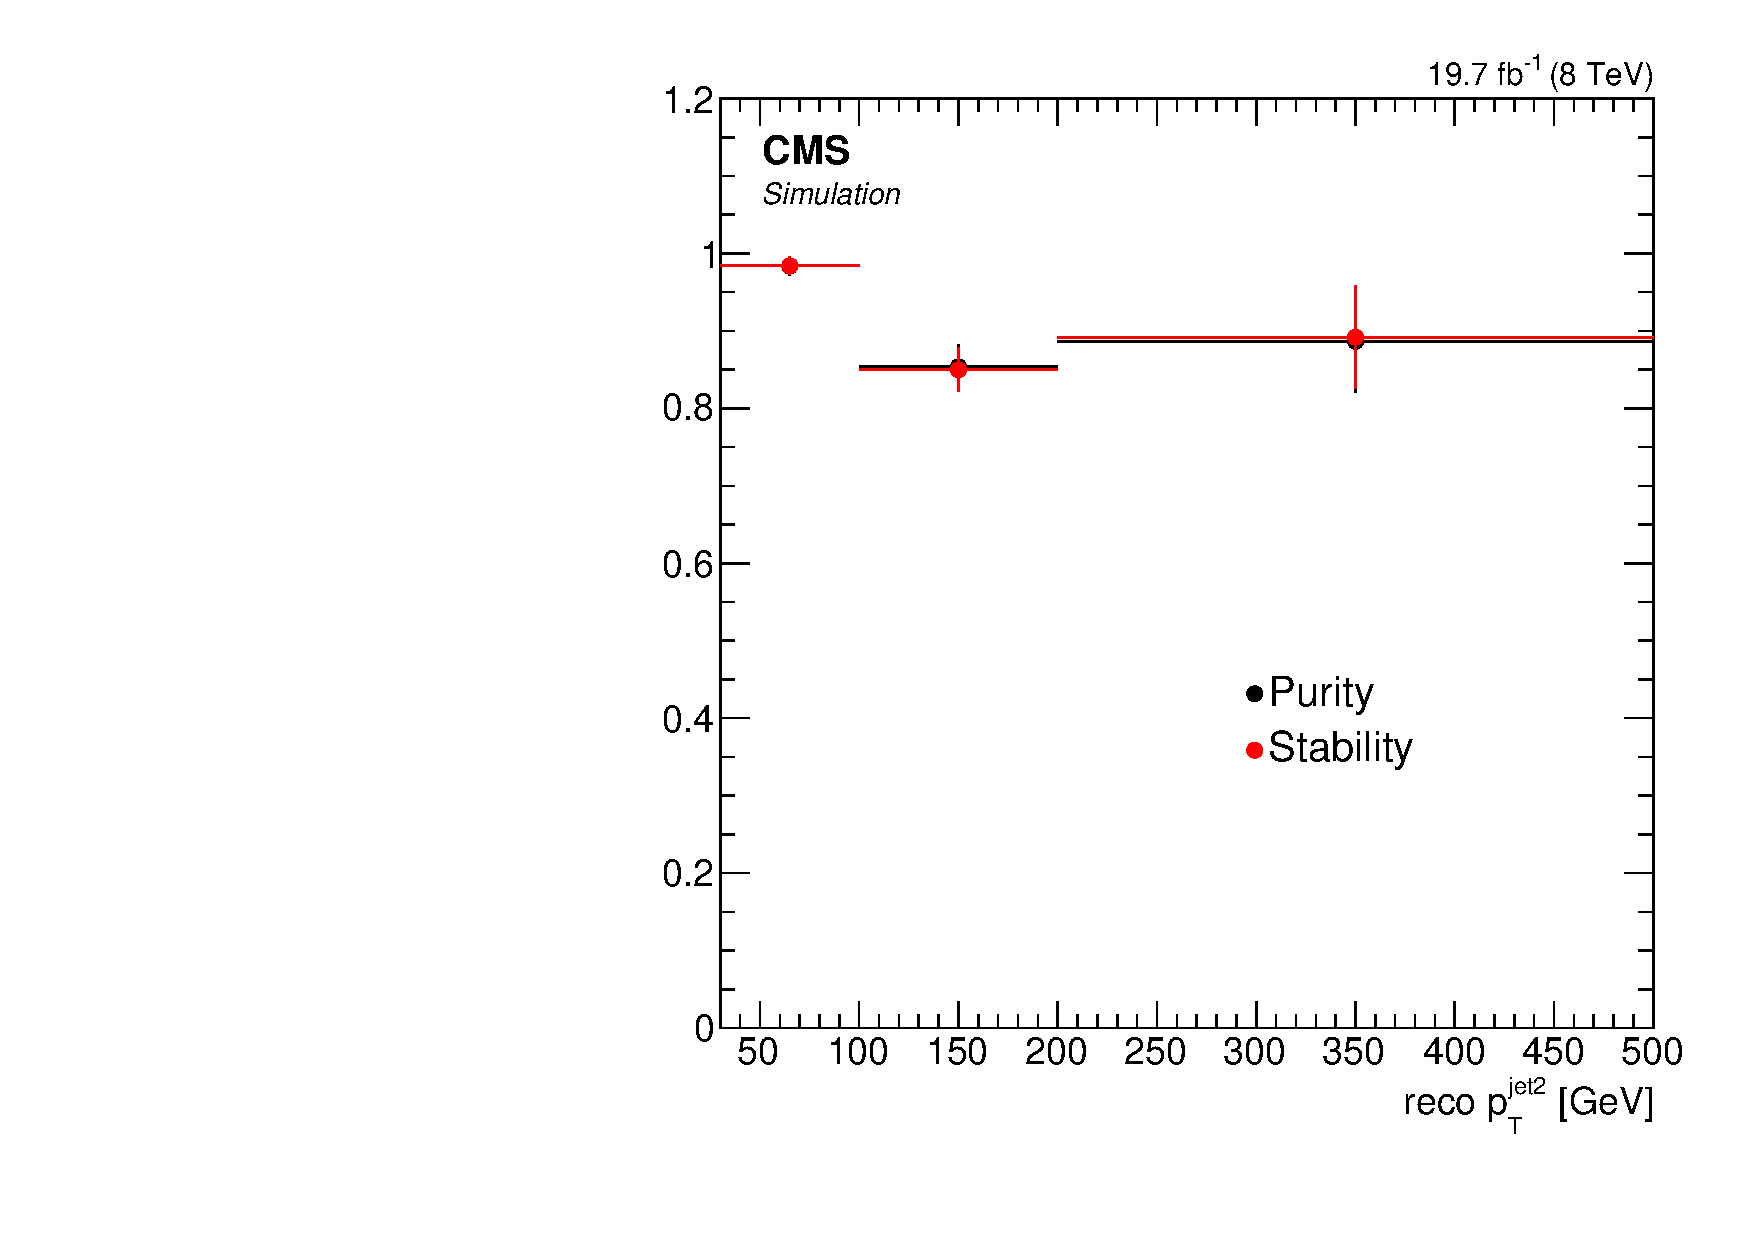
\includegraphics[width=0.8\cmsFigWidth]{Figures/Unfolding/BinMigration/PurityStability_2e2m_PtJet2_Mad}
    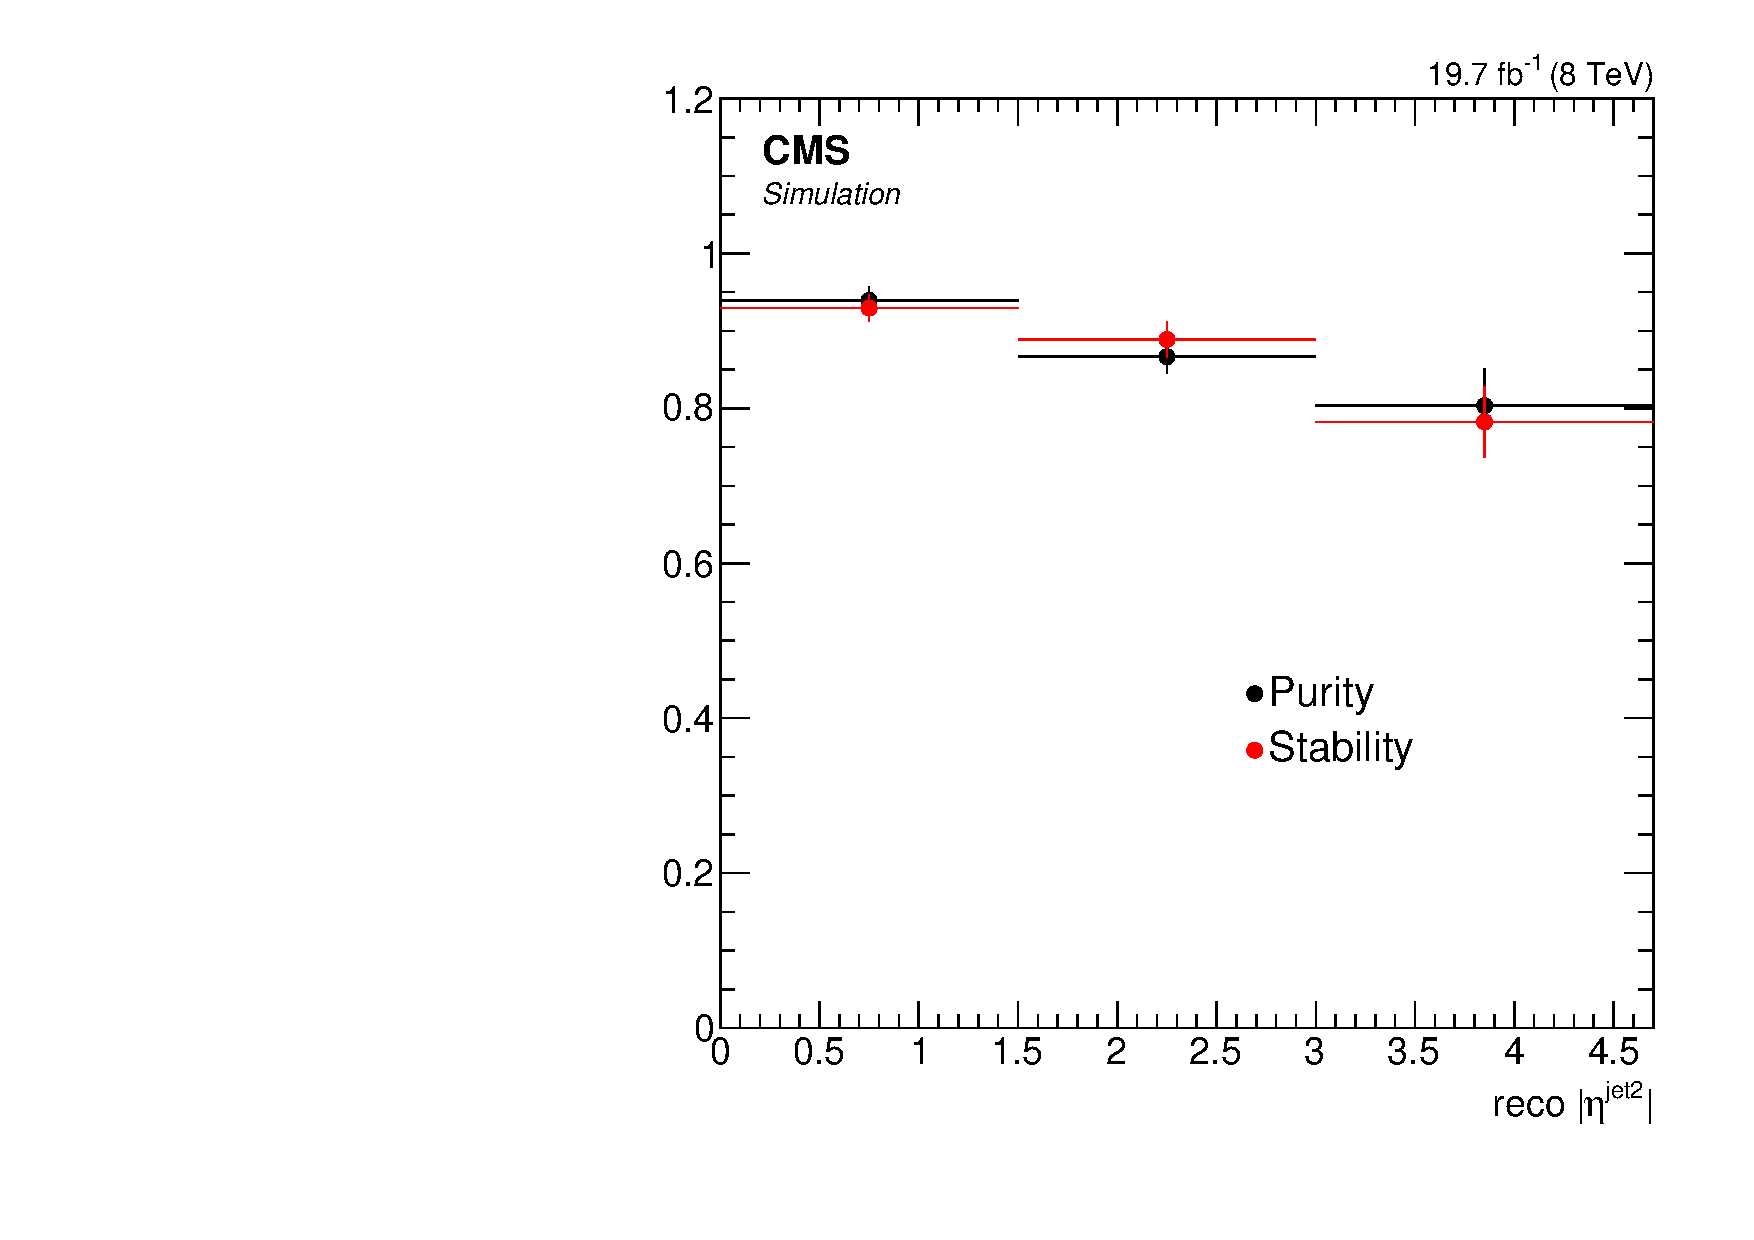
\includegraphics[width=0.8\cmsFigWidth]{Figures/Unfolding/BinMigration/PurityStability_4m_EtaJet2_Mad}
    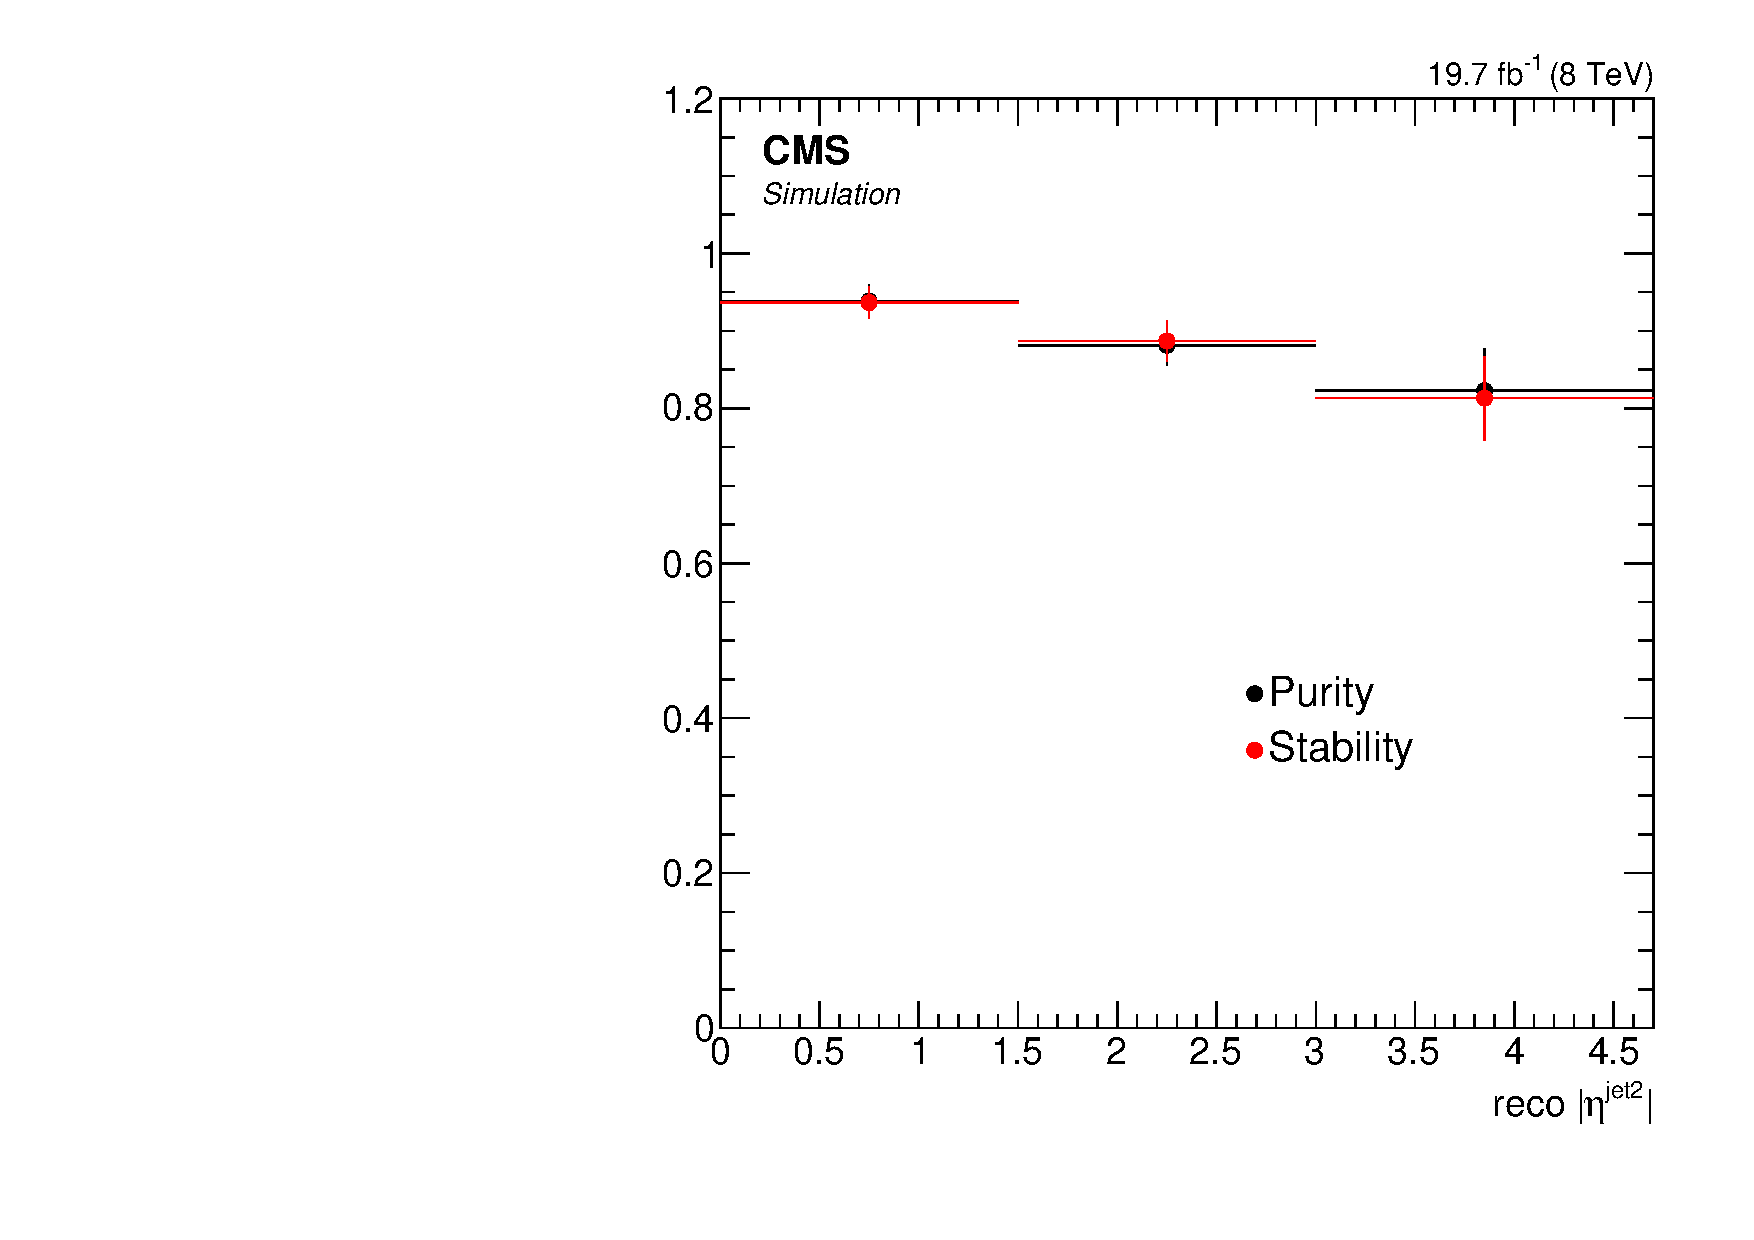
\includegraphics[width=0.8\cmsFigWidth]{Figures/Unfolding/BinMigration/PurityStability_4e_EtaJet2_Mad}
    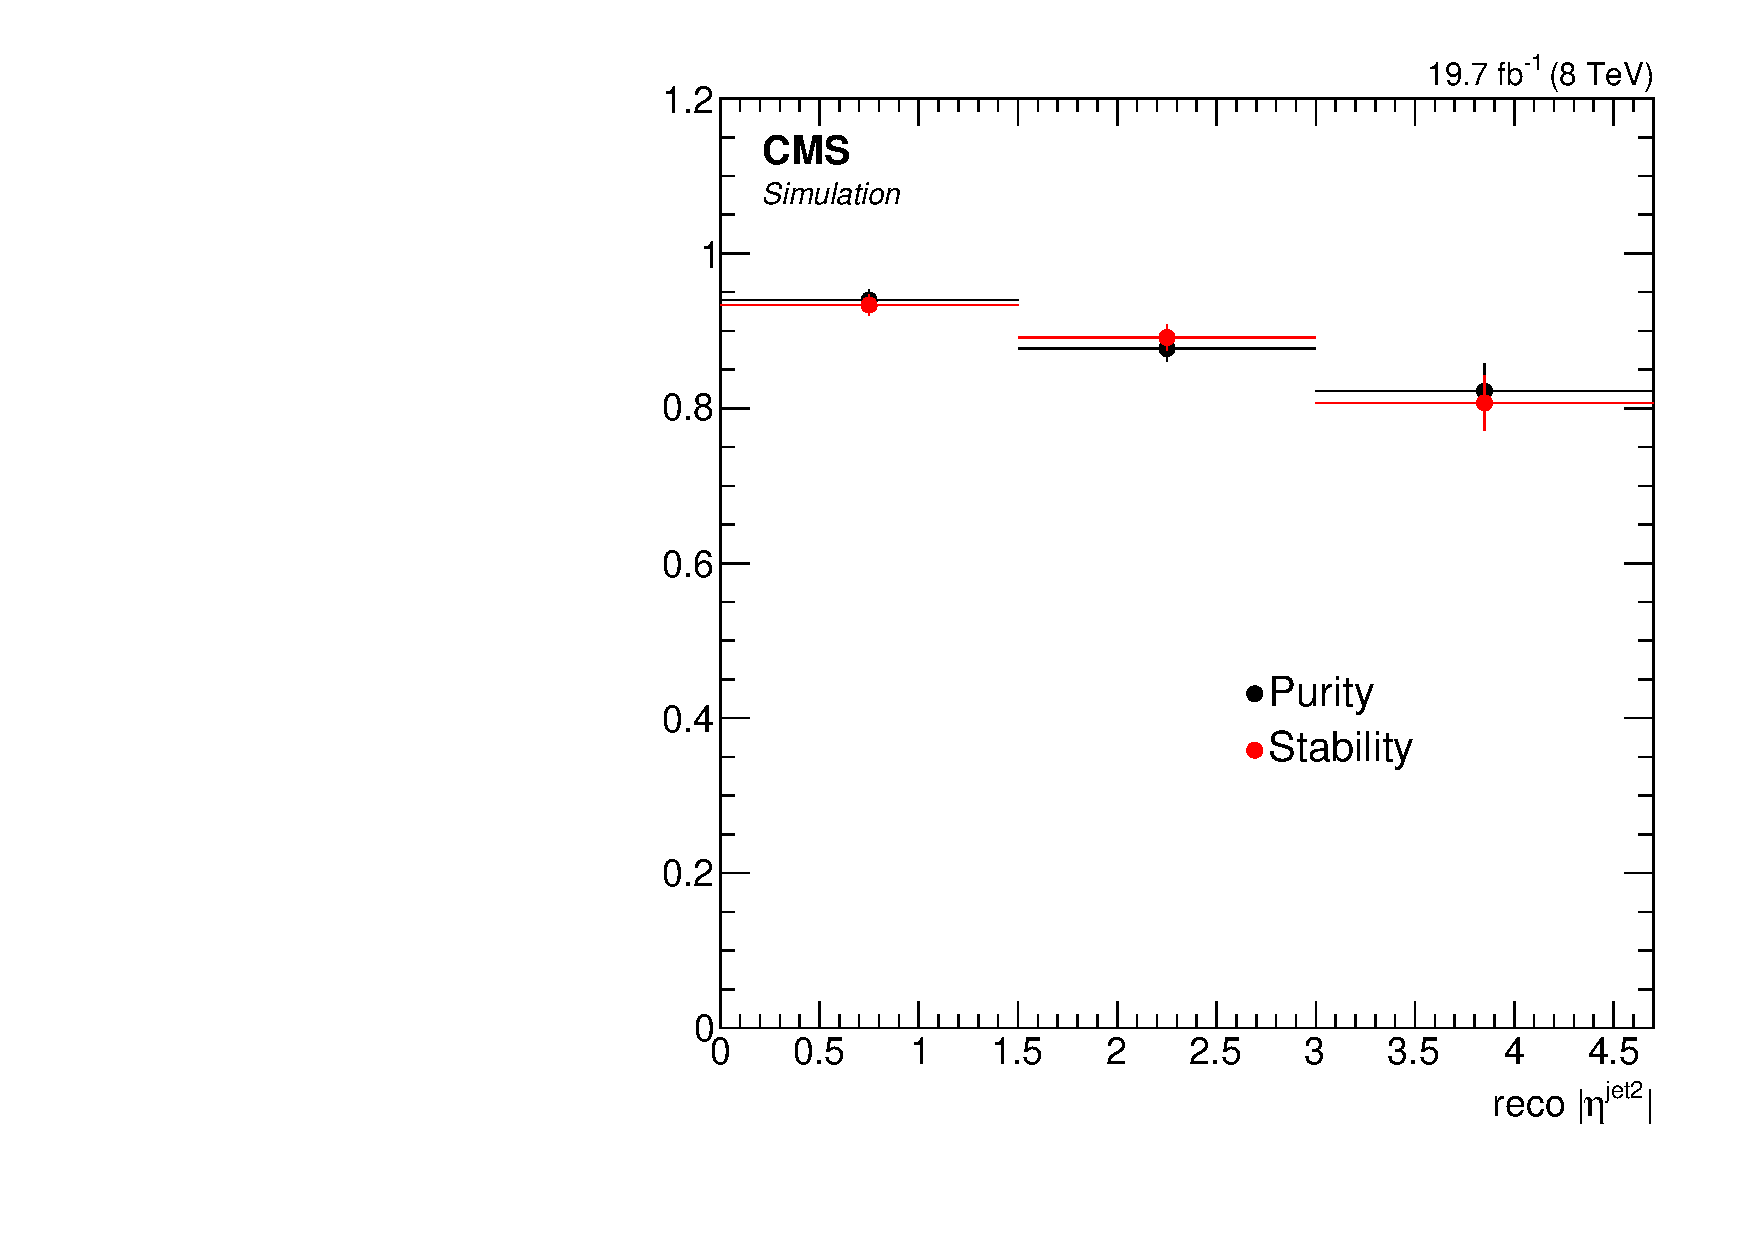
\includegraphics[width=0.8\cmsFigWidth]{Figures/Unfolding/BinMigration/PurityStability_2e2m_EtaJet2_Mad}
 \caption{Purity and stability as a function of the $p_T$ (top) and $\eta$ (bottom) of the second most energetic jet in the event,  for the $4\mu$ (left), $4e$ (center) and $2e2\mu$ (right) final states.}
    \label{fig:ps_jet2}
  \end{center}
\end{figure}

\clearpage
\subsection{Unfolding validation test on Monte Carlo}
Before looking at the data, it is recommended to test the unfolding procedure on MC events alone. 
As first step the consistency of the whole process is checked using the full \texttt{MadGraph} (or \texttt{Powheg}) set of samples,
both for the distribution to be unfolded and the response matrix. If everything is
correctly implemented the unfolded distribution and the generated one should be exactly the
same. Moreover, in order to get meaningful results, the distribution that has to be unfolded must be statistically independent 
from the 2-dimensional response histogram. The \texttt{MadGraph}(\texttt{Powheg}) set is thus split into two samples: one of them
is used to fill the response matrix, while the other one is used to build the distribution to unfold. Finally, in order to compare the effect of employing different signal samples and to be sure the procedure is
independent of the choice of a particular MC, the response matrix from the \texttt{MadGraph} set is applied on the distribution 
obtained using the \texttt{Powheg} set and vice versa. Tests are performed both in the standard and tight fiducial regions and results for the latter case are reported from Figure~\ref{fig:MCtest_Mass1} to Figure~\ref{fig:MCtest_EtaJet22} for the considered distributions, in the three different final states. In each plot the ratio of unfolded over generated
distribution is shown and, as expected, it is unity. \\
Closure tests show that the unfolding procedure doesn't introduce any additional bias and demonstrate its effectiveness. 

%% , as it is shown in figures~\ref{fig:FullMad_4e}, ~\ref{fig:FullMad_4m} and ~\ref{fig:FullMad_2e2m} (or in figures~\ref{fig:FullPow_4e}, ~\ref{fig:FullPow_4m} and ~\ref{fig:FullPow_2e2m} for \texttt{Powheg}) for the four considered distributions, in the three different final 
%% states. In each plot the ratio of unfolded over generated
%% distribution is shown and, as expected, it is unity.\\

%% Figures~\ref{fig:HalfMad_4e}, ~\ref{fig:HalfMad_4m} and ~\ref{fig:HalfMad_2e2m}(~\ref{fig:HalfPow_4e}, ~\ref{fig:HalfPow_4m} and ~\ref{fig:HalfPow_2e2m}) show the result of this closure test.\\
%%  Results are reported in figures~\ref{fig:MadMat_PowDist_4e} -~\ref{fig:MadMat_PowDist_4m} 
%% -~\ref{fig:MadMat_PowDist_2e2m} and~\ref{fig:PowMat_MadDist_4e} -~\ref{fig:PowMat_MadDist_4m} -~\ref{fig:PowMat_MadDist_2e2m}.\\


\begin{figure}[hbtp]
  \begin{center}
    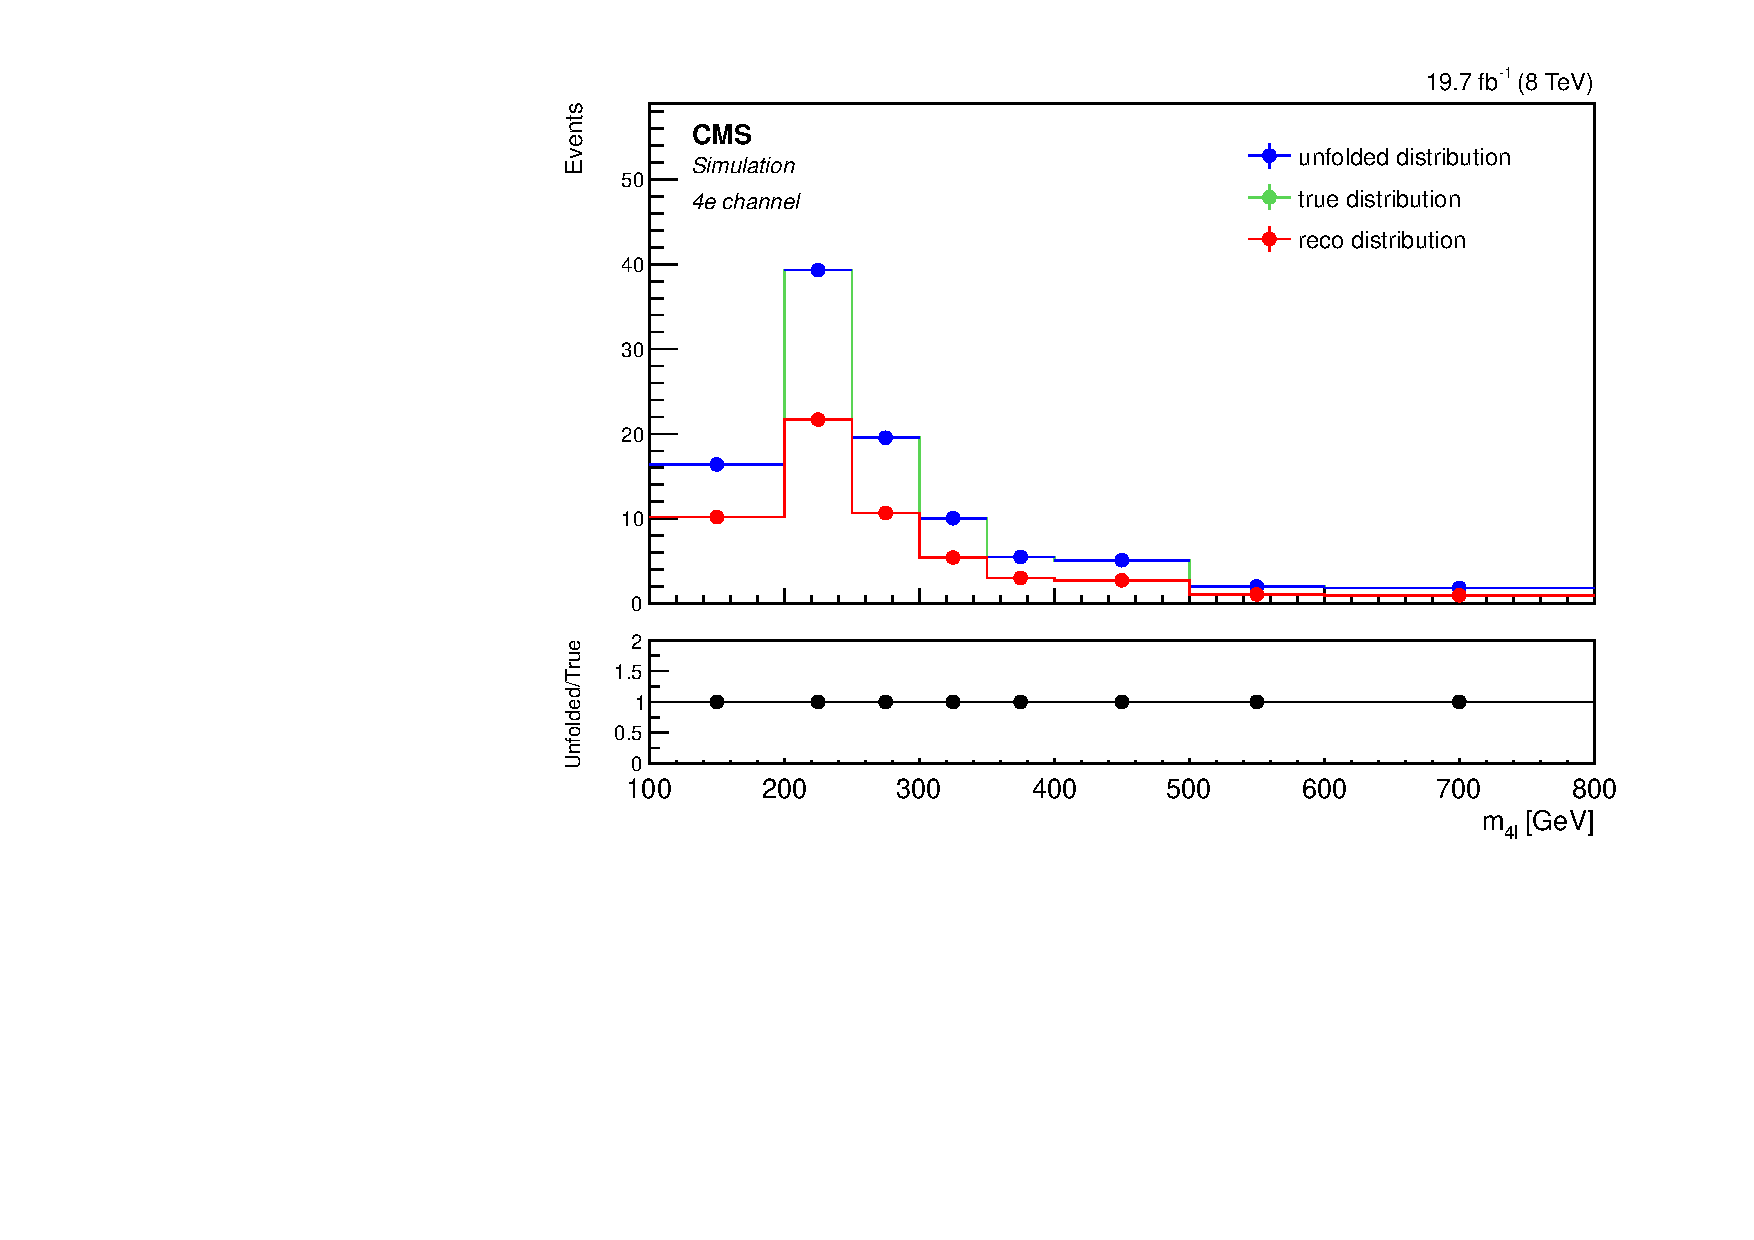
\includegraphics[width=0.8\cmsFigWidth]{Figures/Unfolding/MCTests/Mass_ZZTo4e_MadMatrix_MadDistr_FullSample_fr}     
    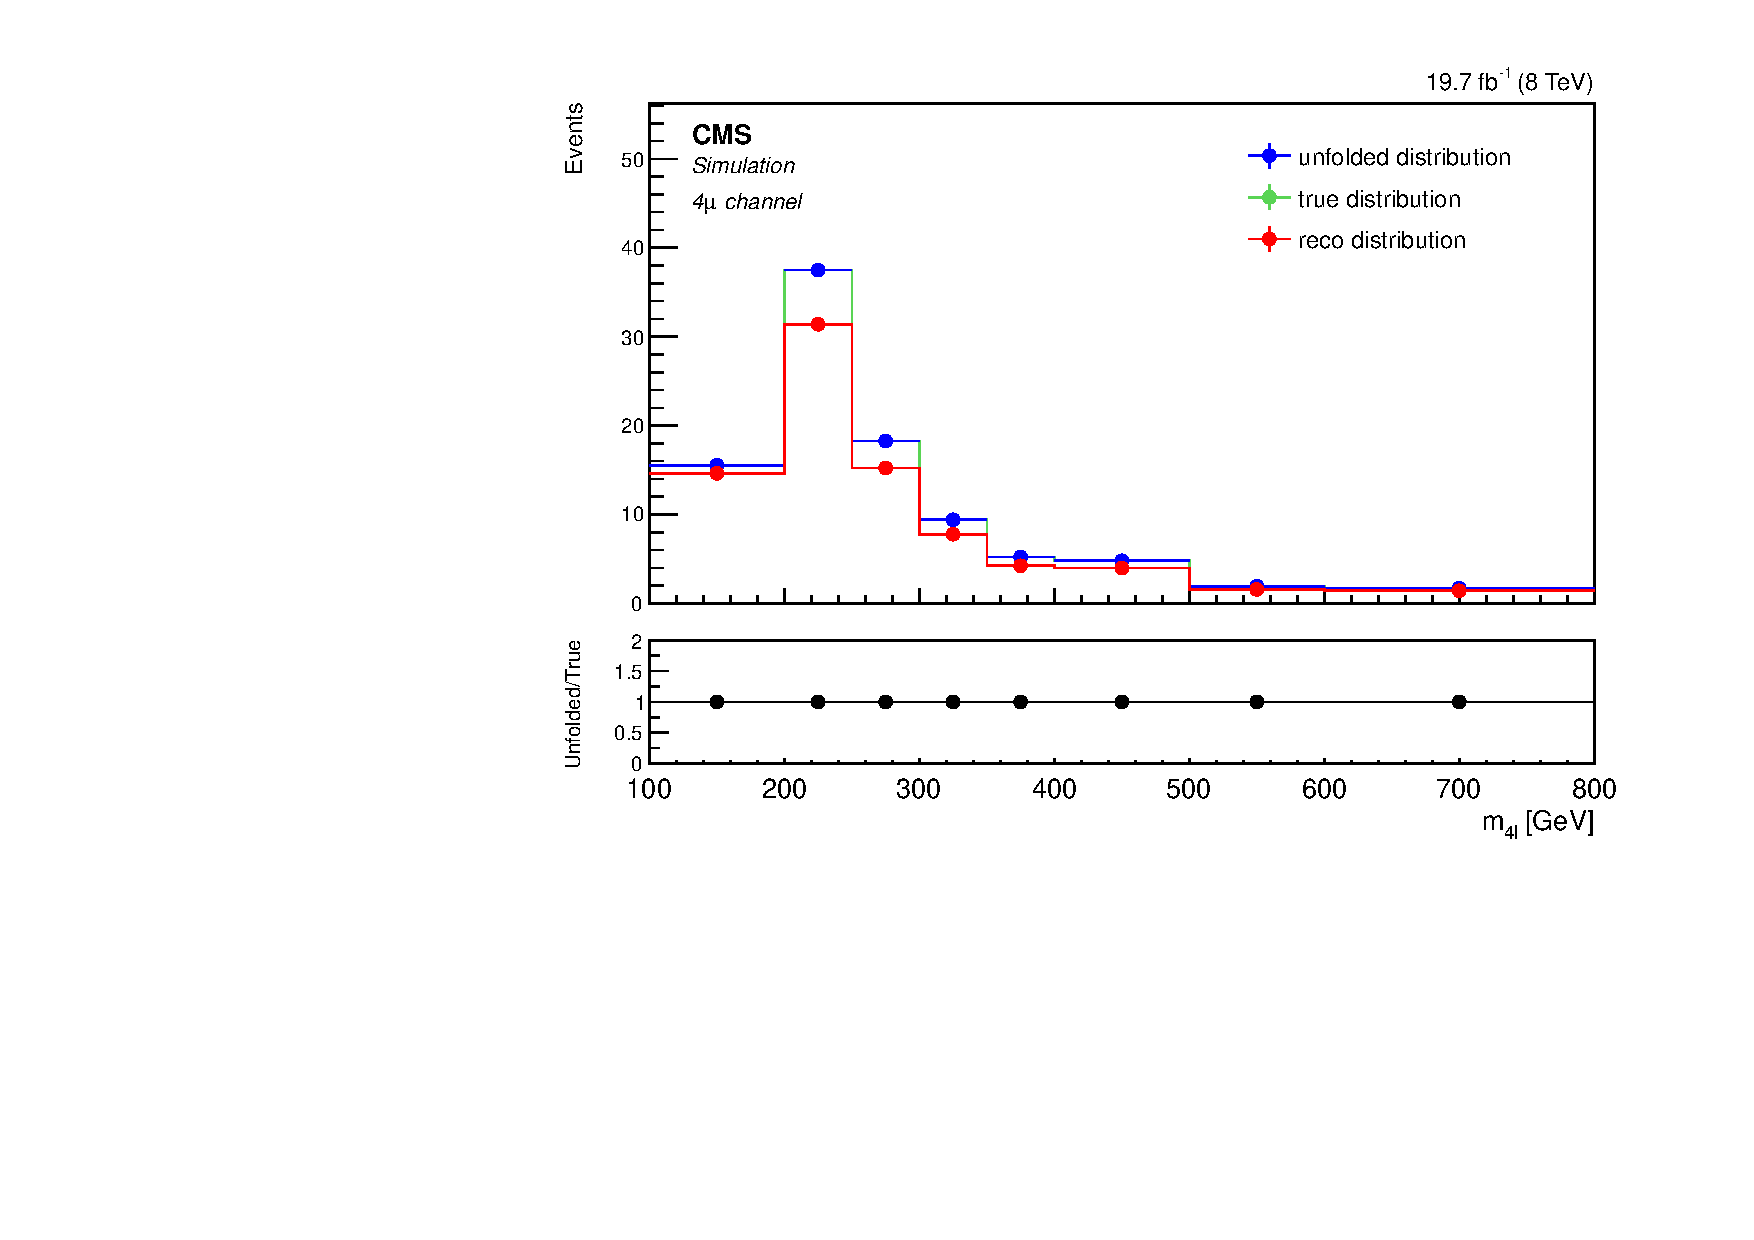
\includegraphics[width=0.8\cmsFigWidth]{Figures/Unfolding/MCTests/Mass_ZZTo4m_MadMatrix_MadDistr_FullSample_fr}     
    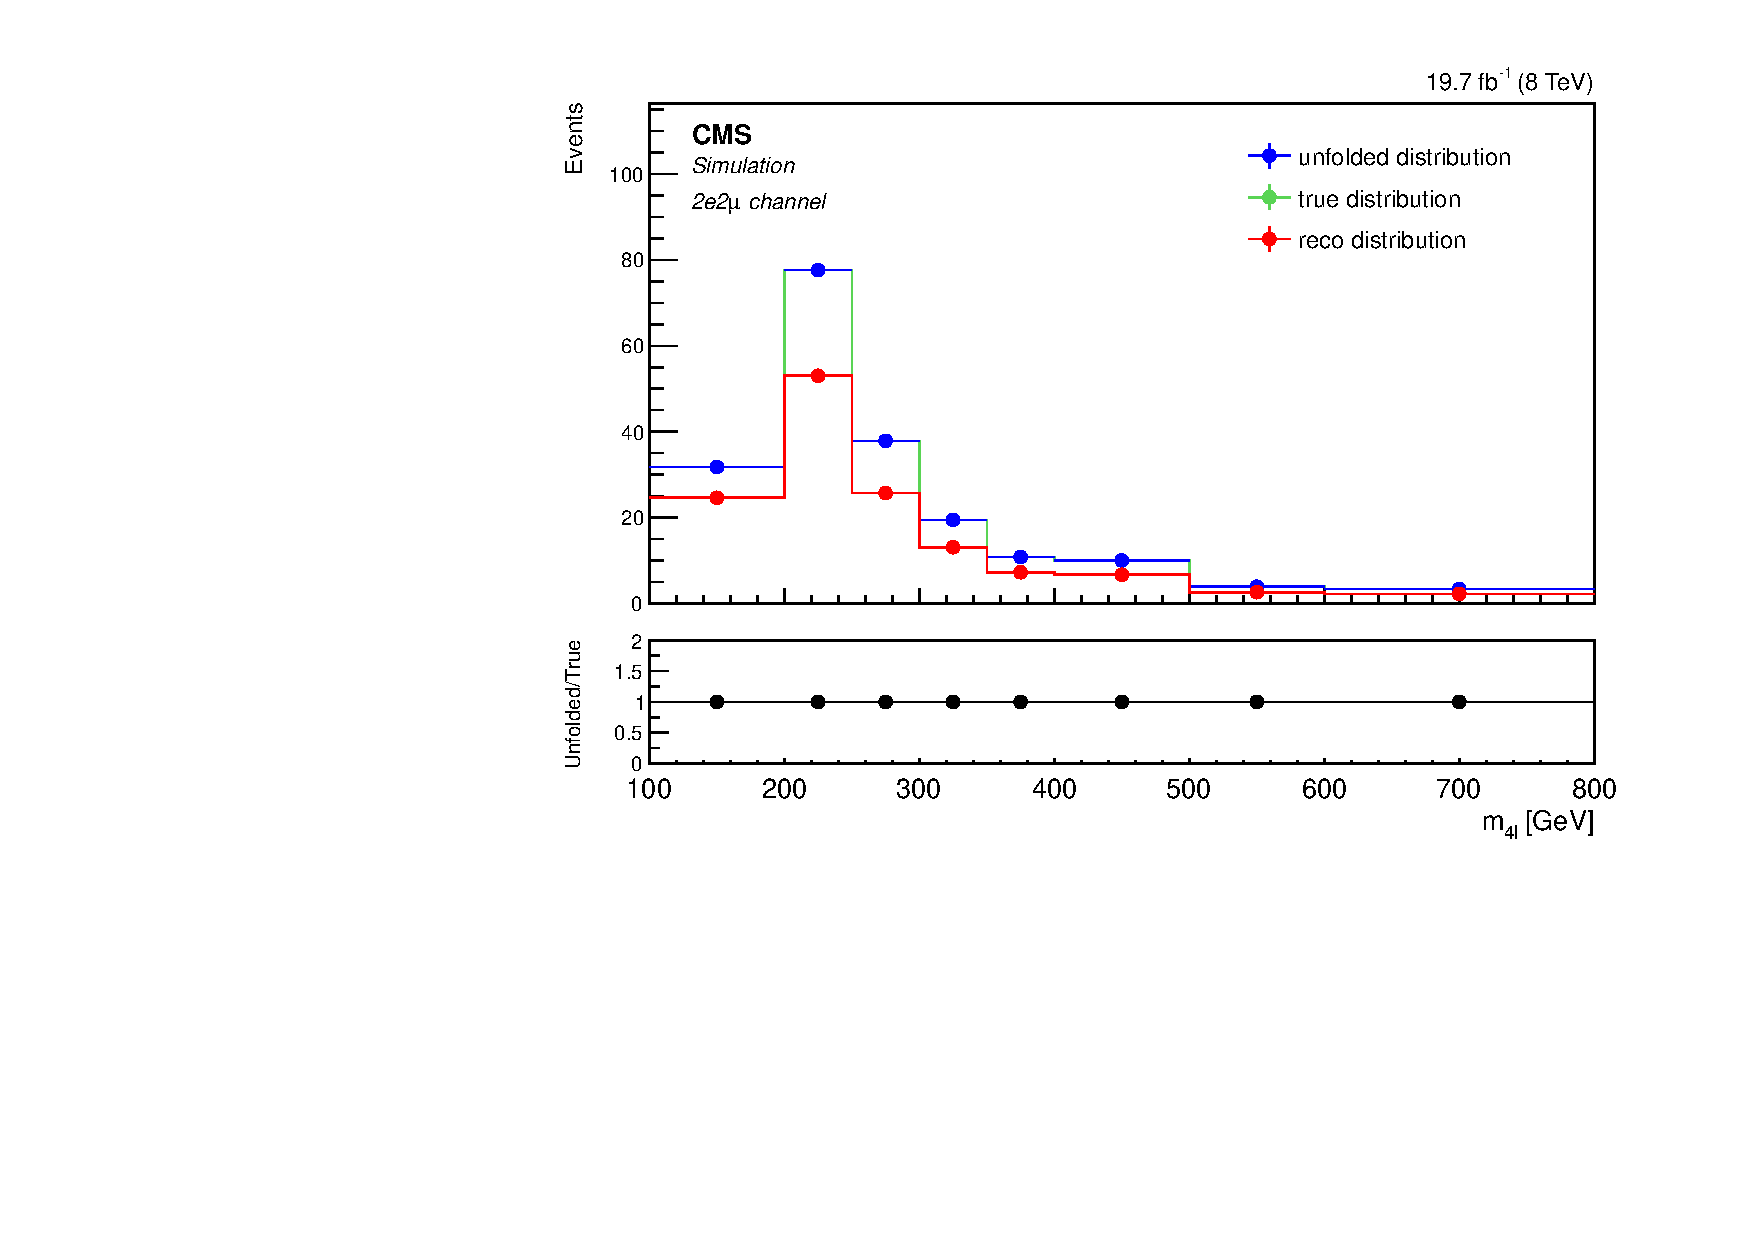
\includegraphics[width=0.8\cmsFigWidth]{Figures/Unfolding/MCTests/Mass_ZZTo2e2m_MadMatrix_MadDistr_FullSample_fr}
     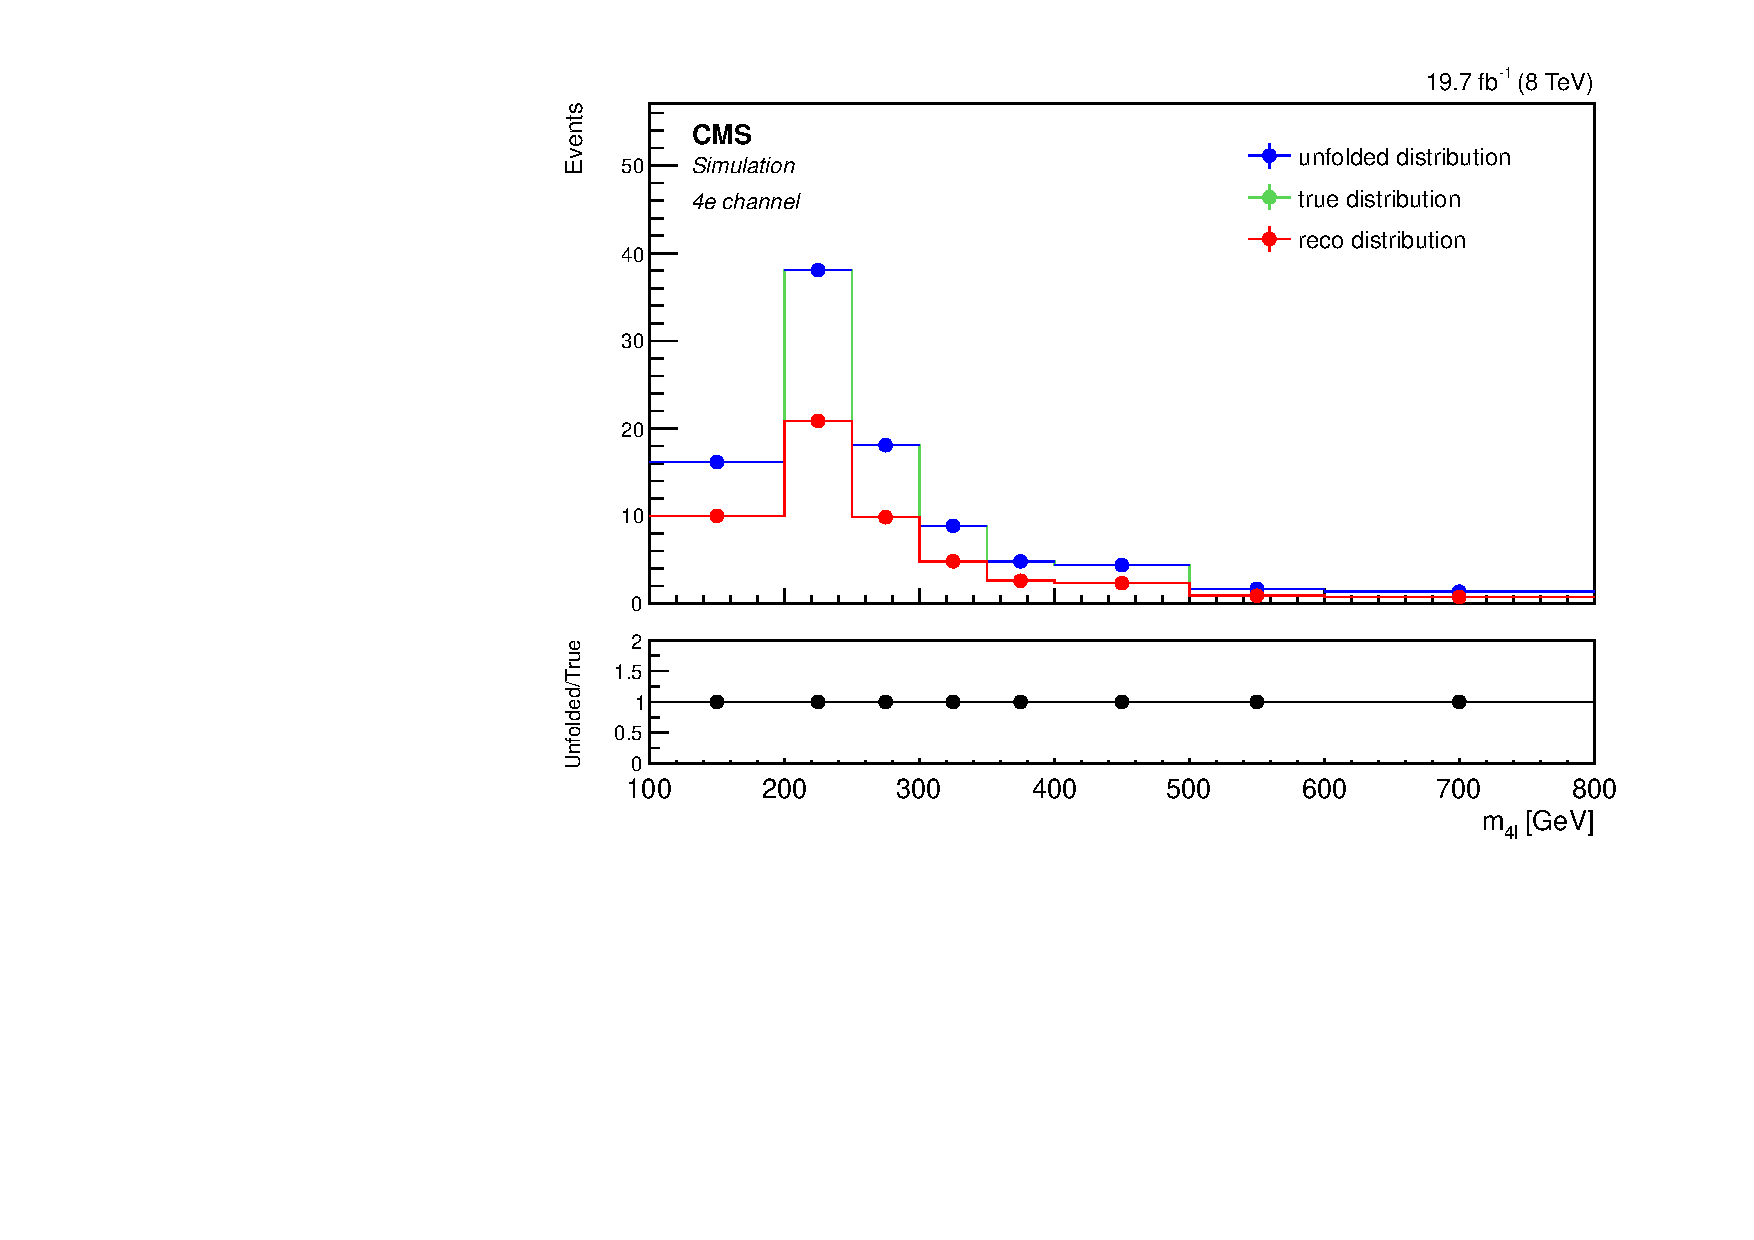
\includegraphics[width=0.8\cmsFigWidth]{Figures/Unfolding/MCTests/Mass_ZZTo4e_PowMatrix_PowDistr_FullSample_fr}     
    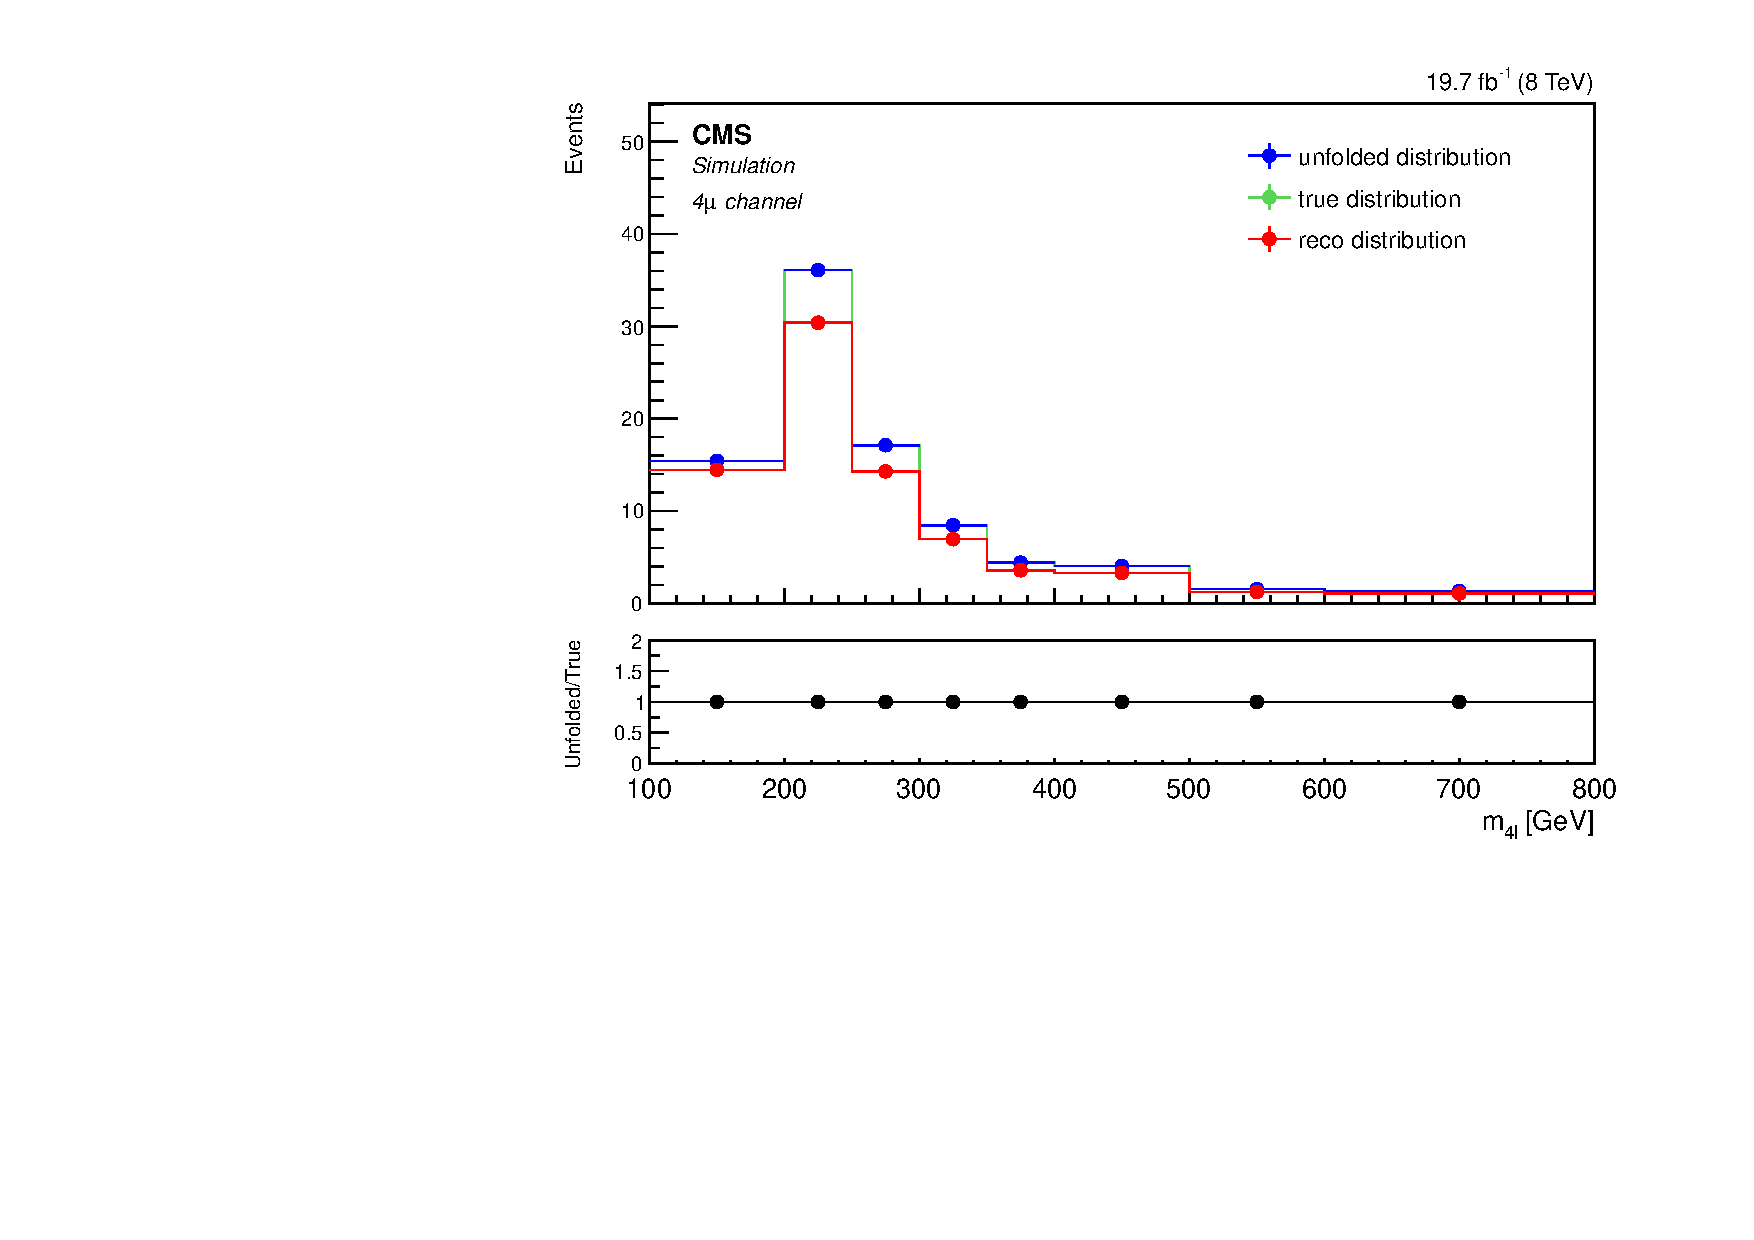
\includegraphics[width=0.8\cmsFigWidth]{Figures/Unfolding/MCTests/Mass_ZZTo4m_PowMatrix_PowDistr_FullSample_fr}     
    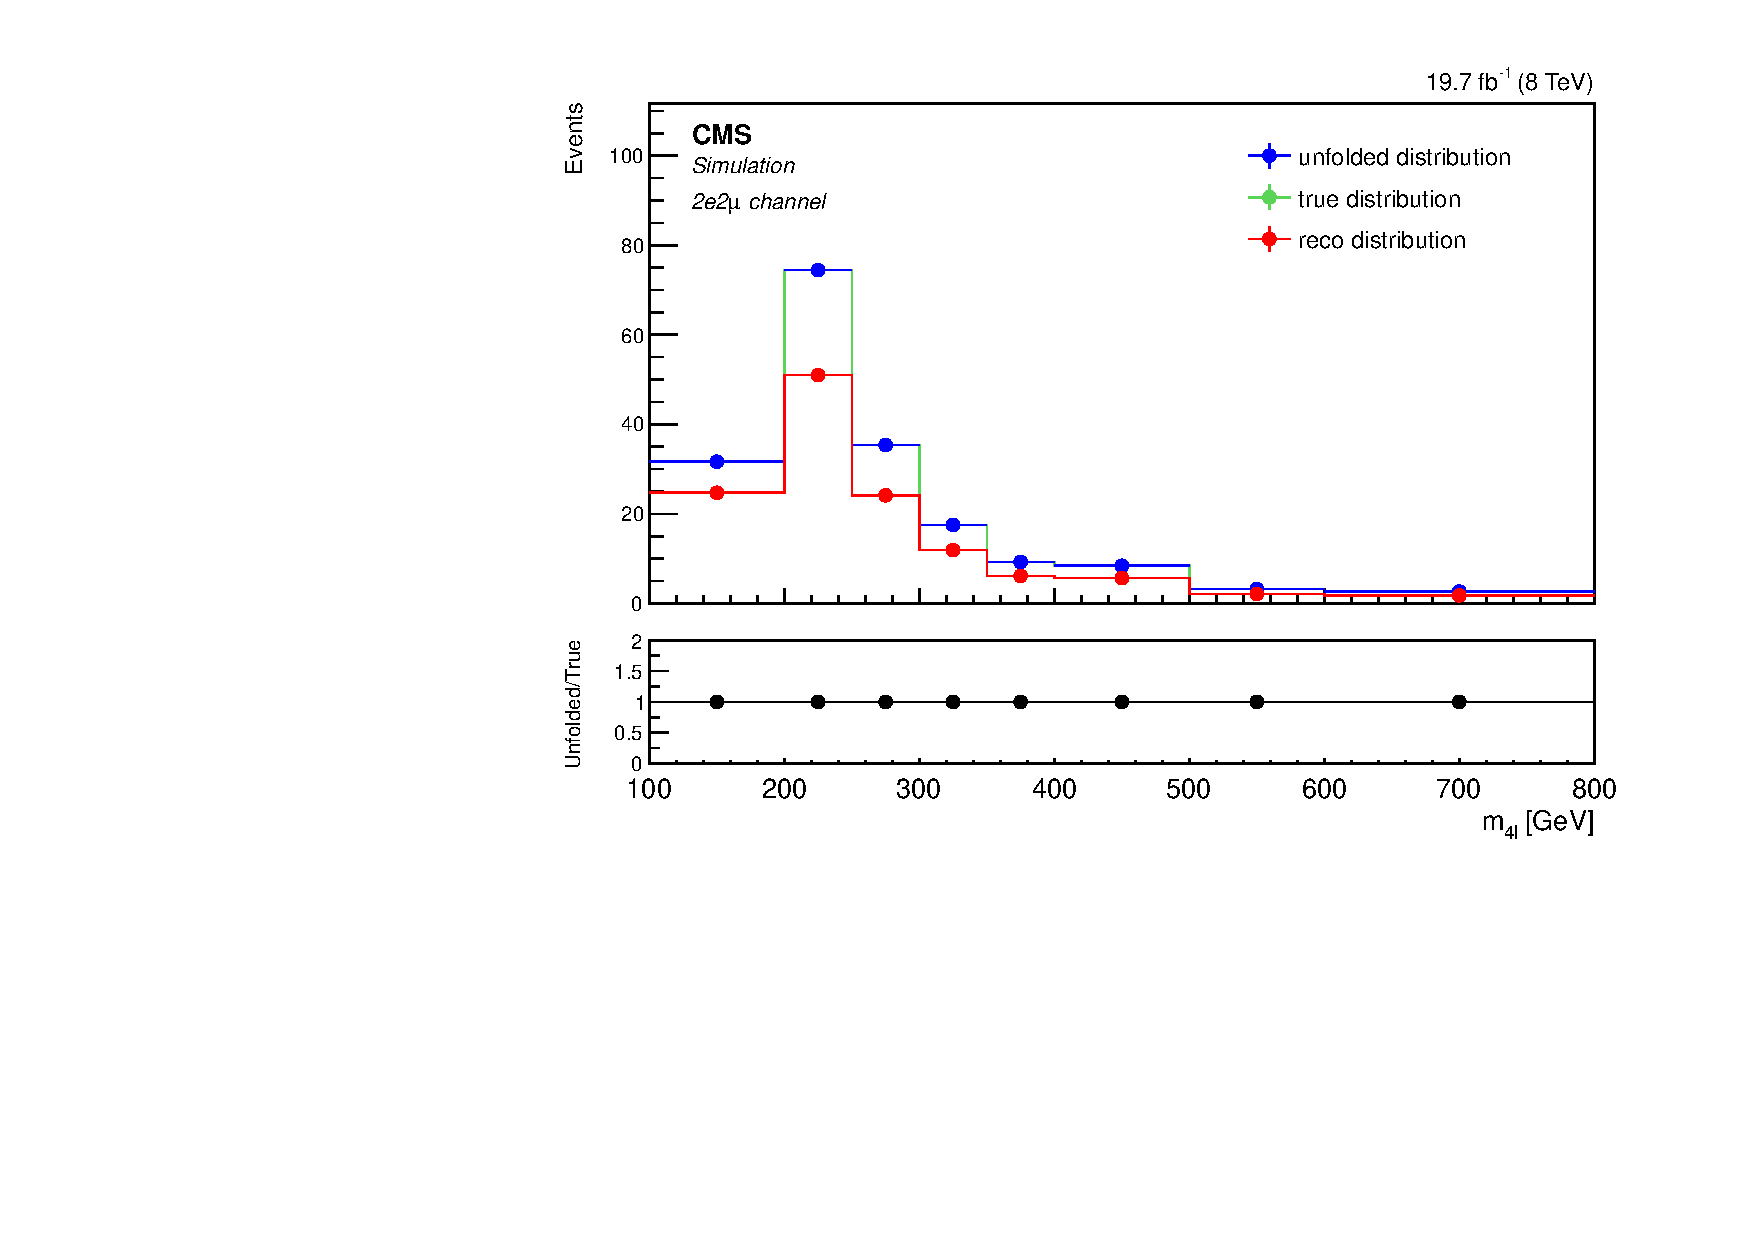
\includegraphics[width=0.8\cmsFigWidth]{Figures/Unfolding/MCTests/Mass_ZZTo2e2m_PowMatrix_PowDistr_FullSample_fr}      
    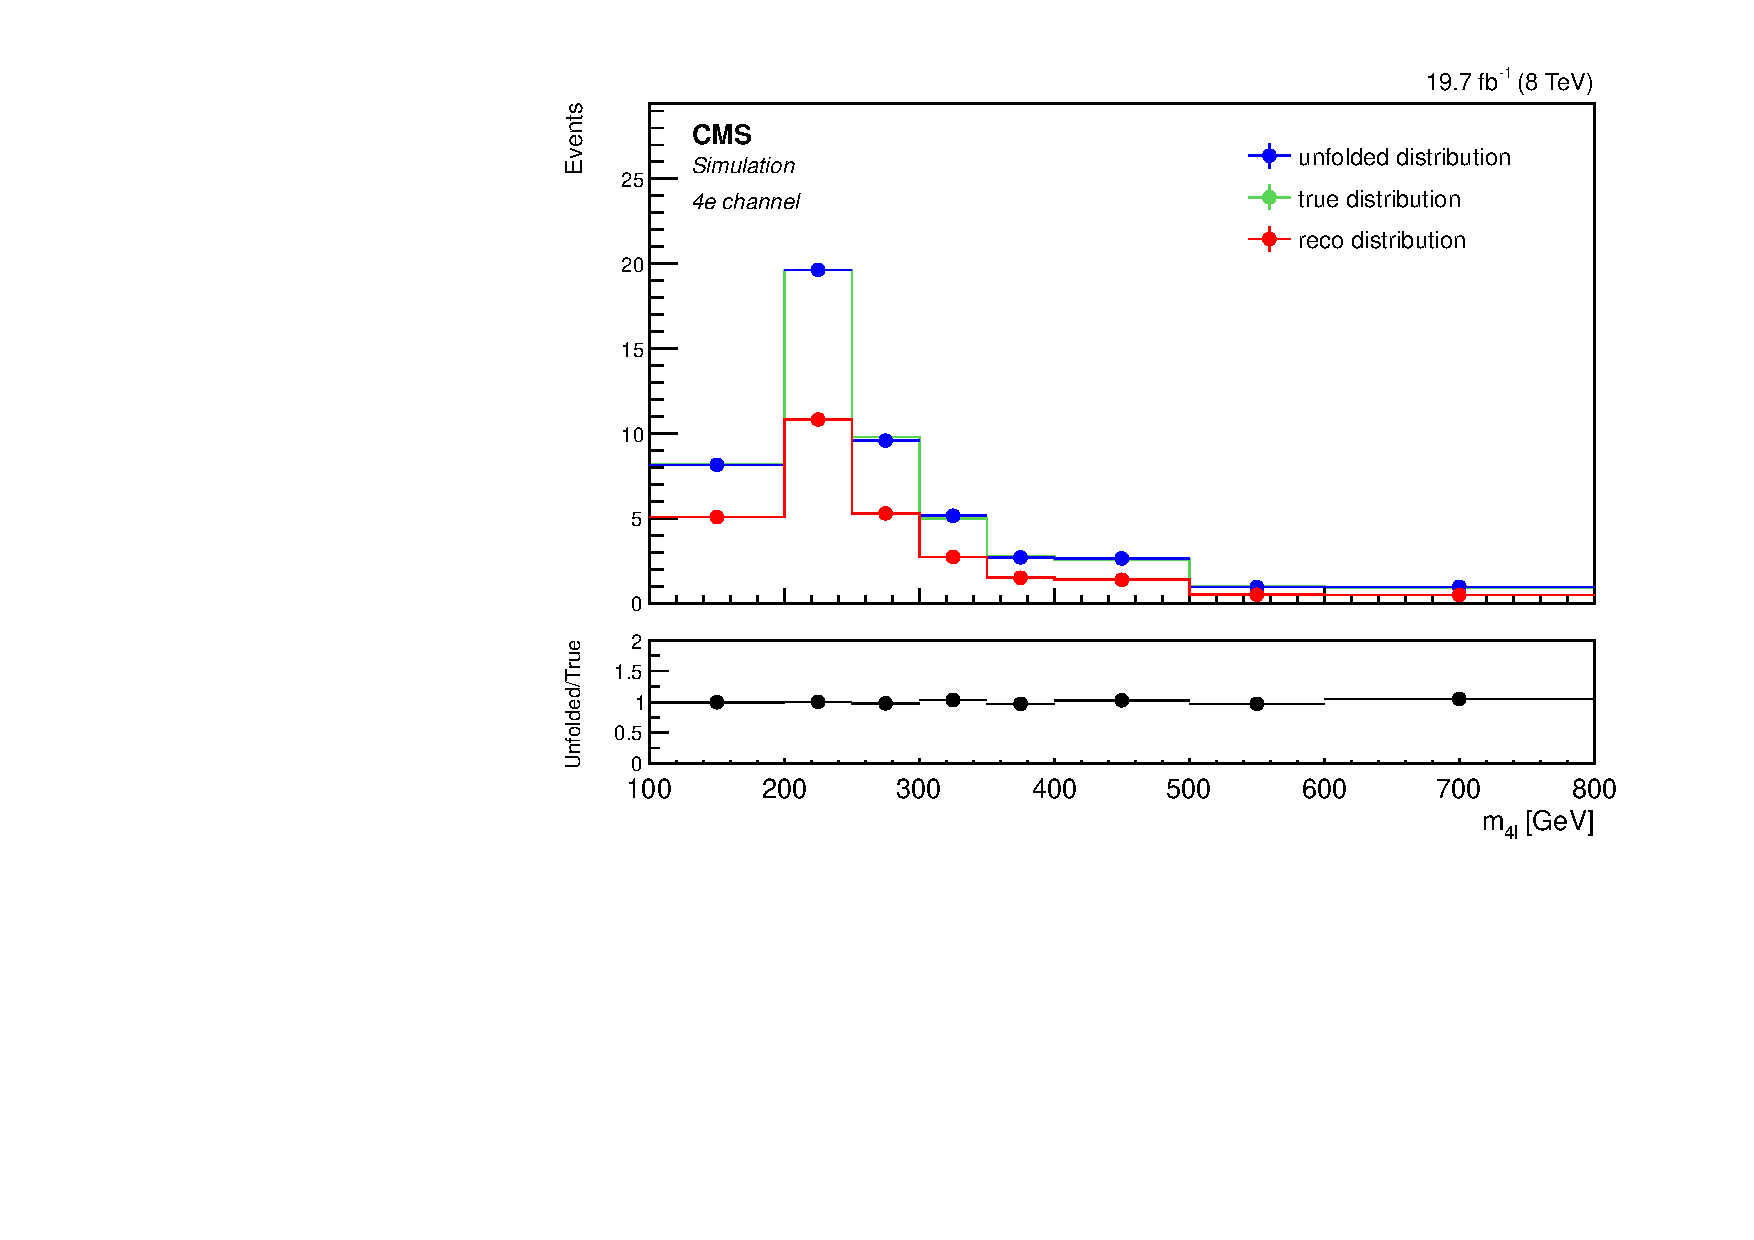
\includegraphics[width=0.8\cmsFigWidth]{Figures/Unfolding/MCTests/Mass_ZZTo4e_MadMatrix_MadDistr_HalfSample_fr}     
    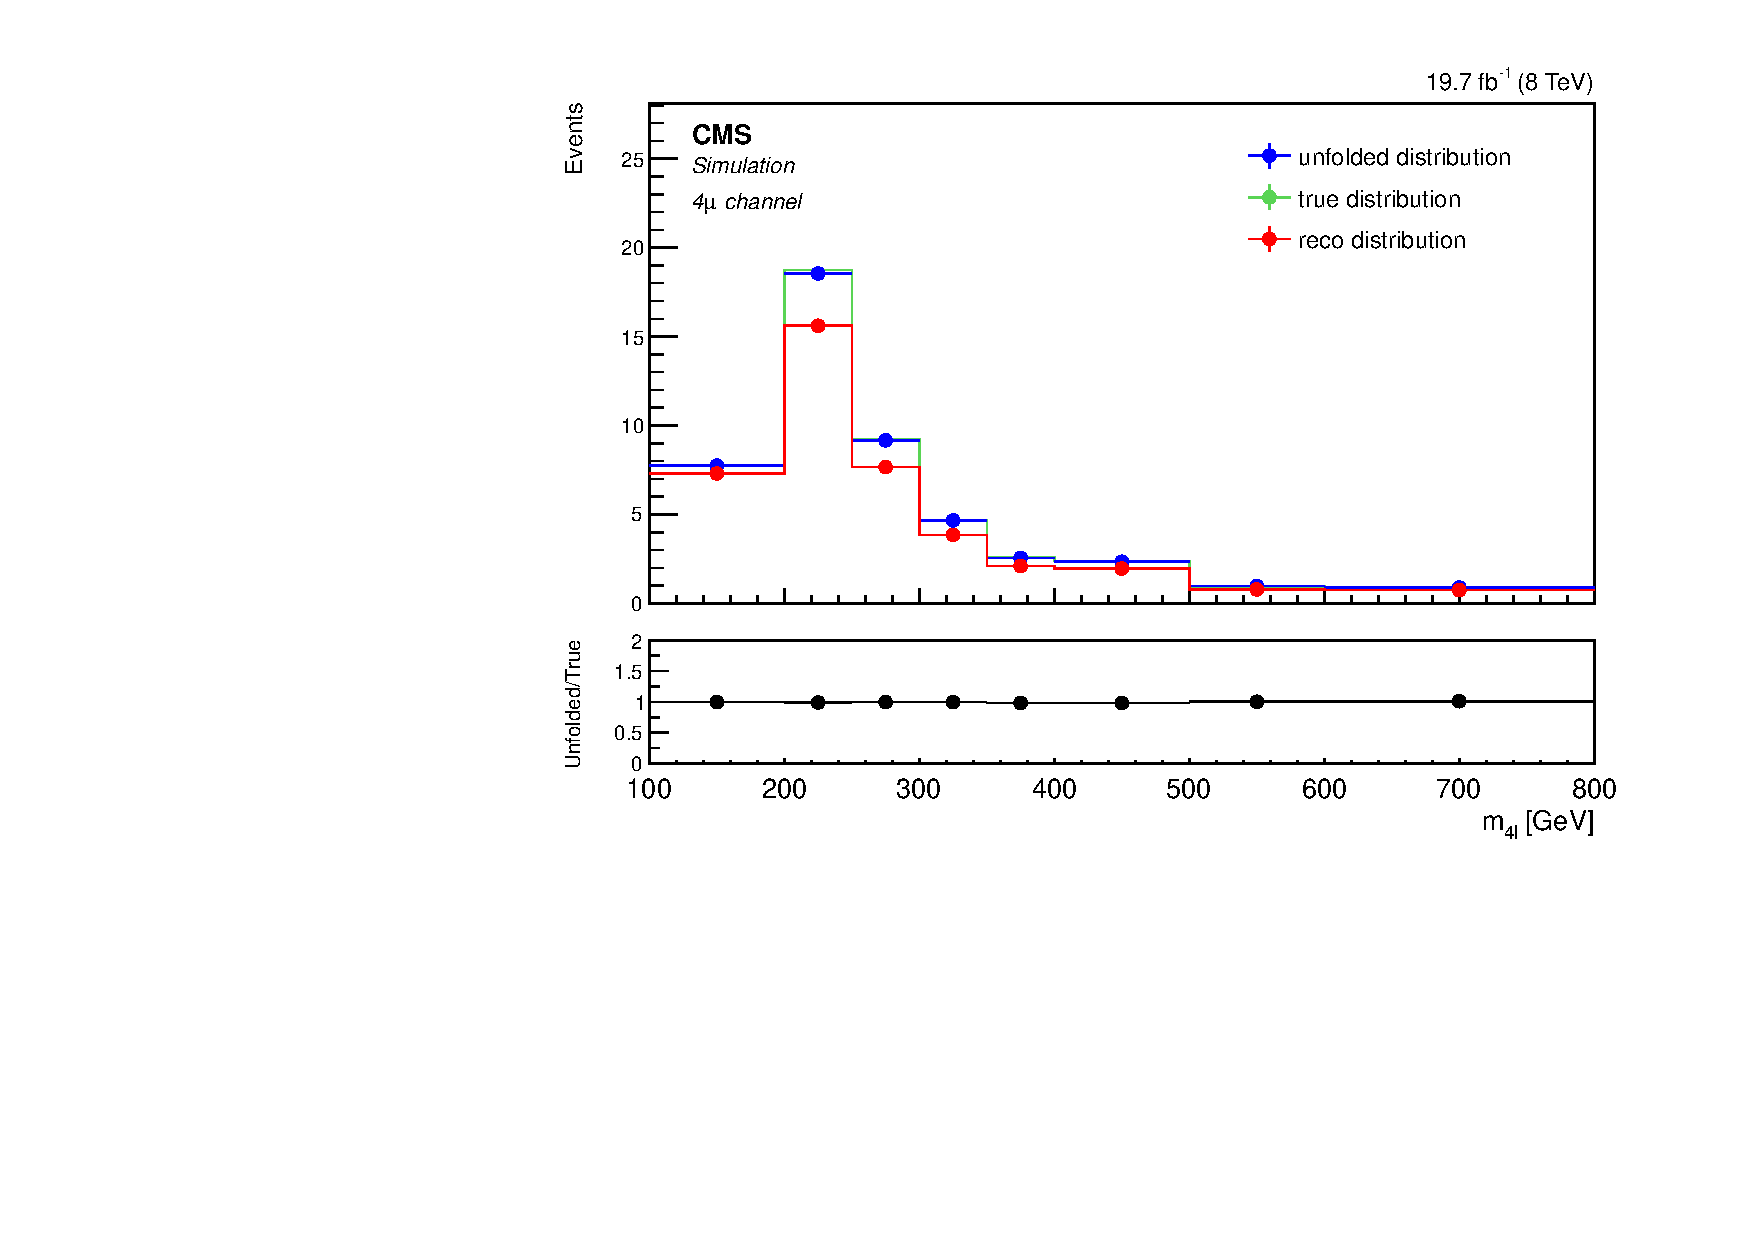
\includegraphics[width=0.8\cmsFigWidth]{Figures/Unfolding/MCTests/Mass_ZZTo4m_MadMatrix_MadDistr_HalfSample_fr}     
    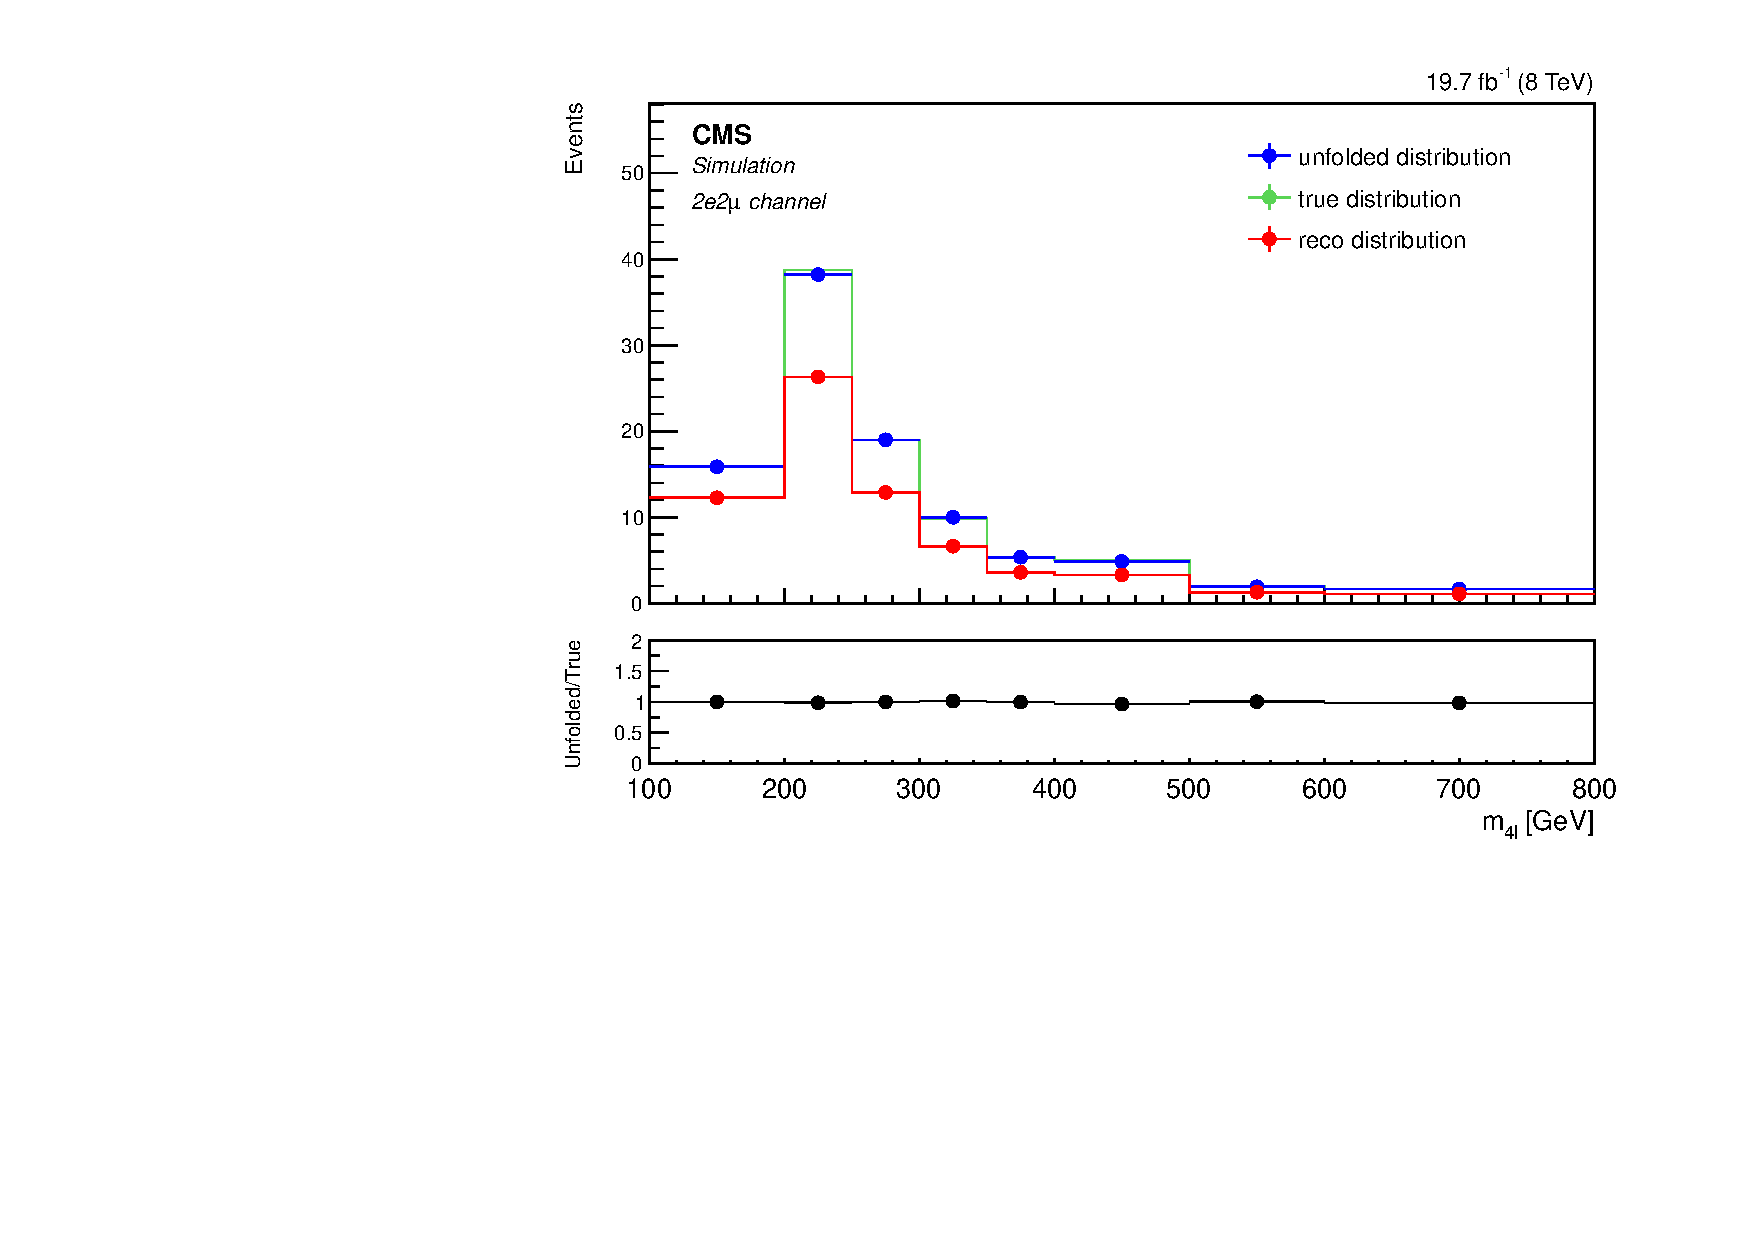
\includegraphics[width=0.8\cmsFigWidth]{Figures/Unfolding/MCTests/Mass_ZZTo2e2m_MadMatrix_MadDistr_HalfSample_fr}     
    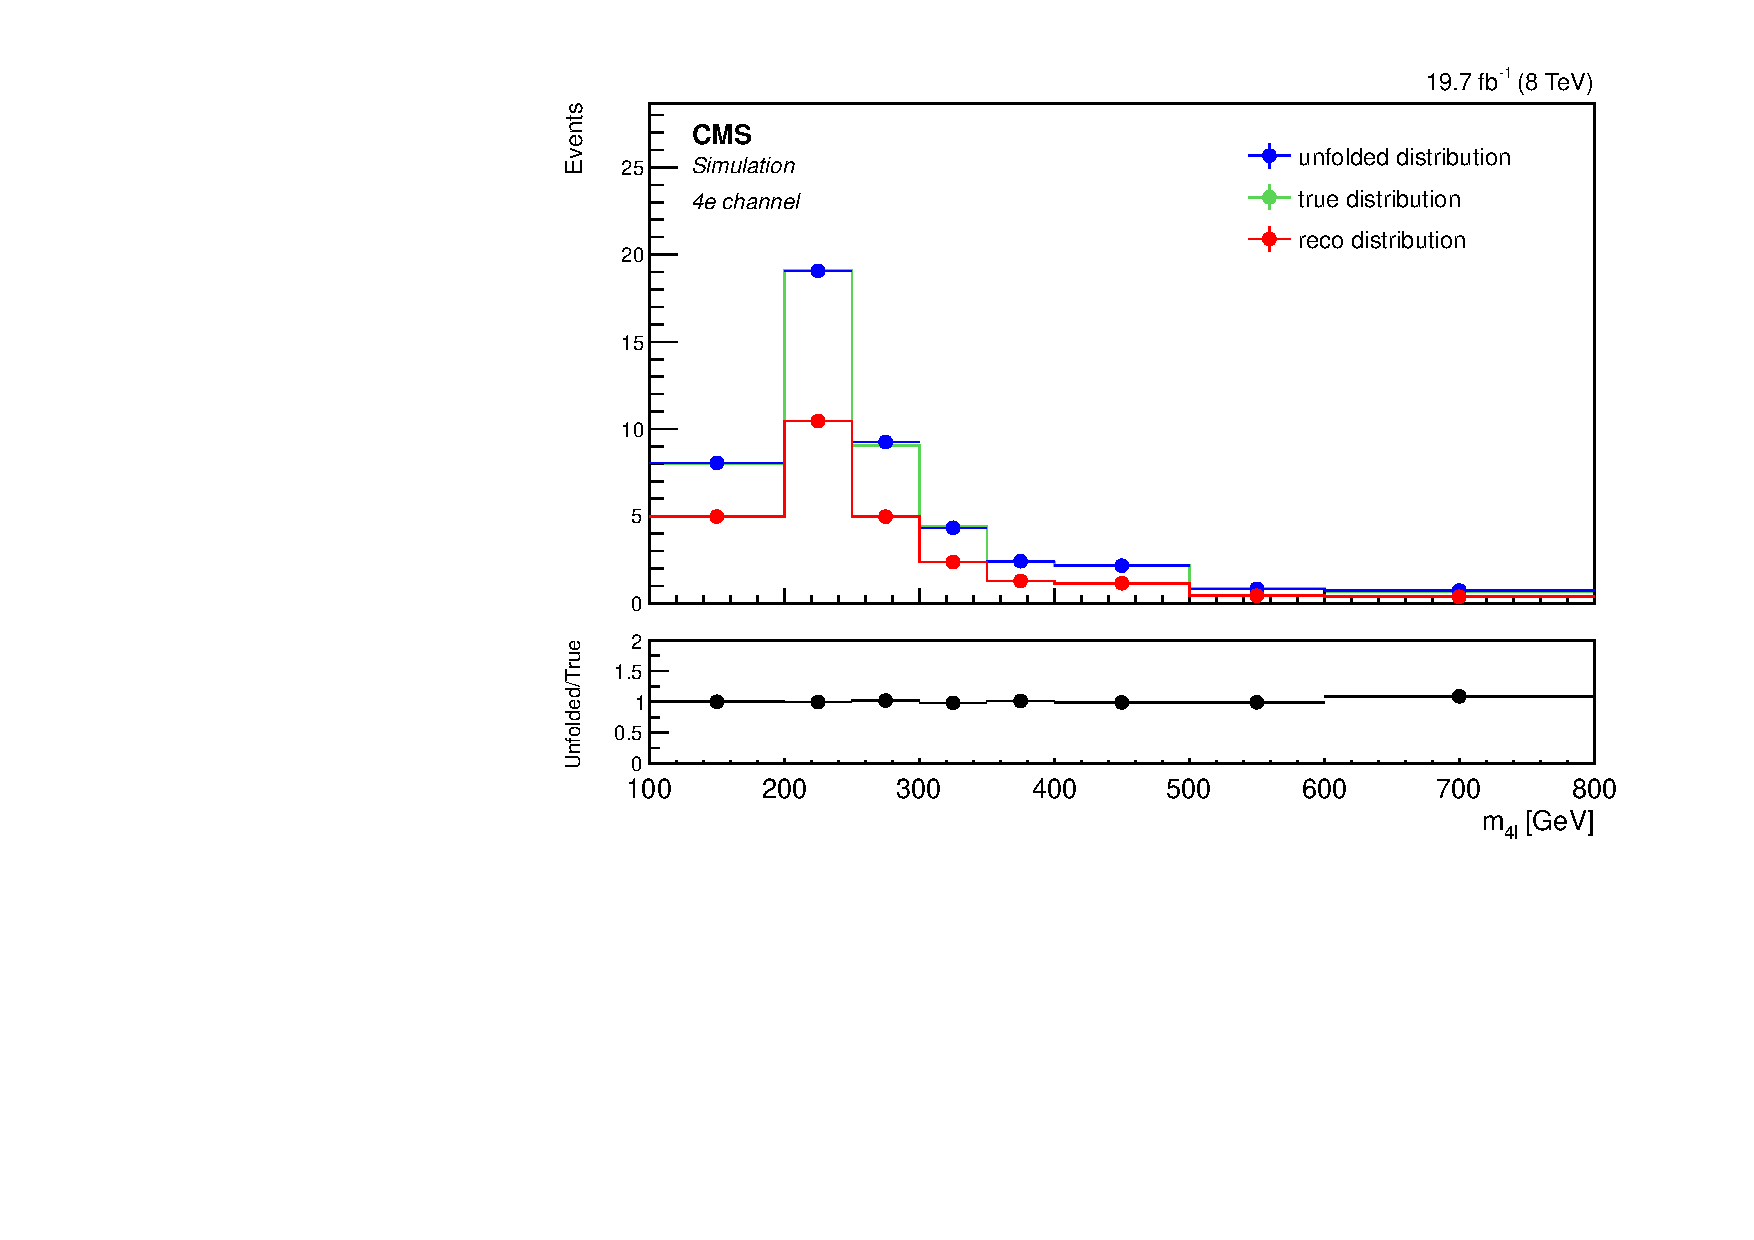
\includegraphics[width=0.8\cmsFigWidth]{Figures/Unfolding/MCTests/Mass_ZZTo4e_PowMatrix_PowDistr_HalfSample_fr}     
    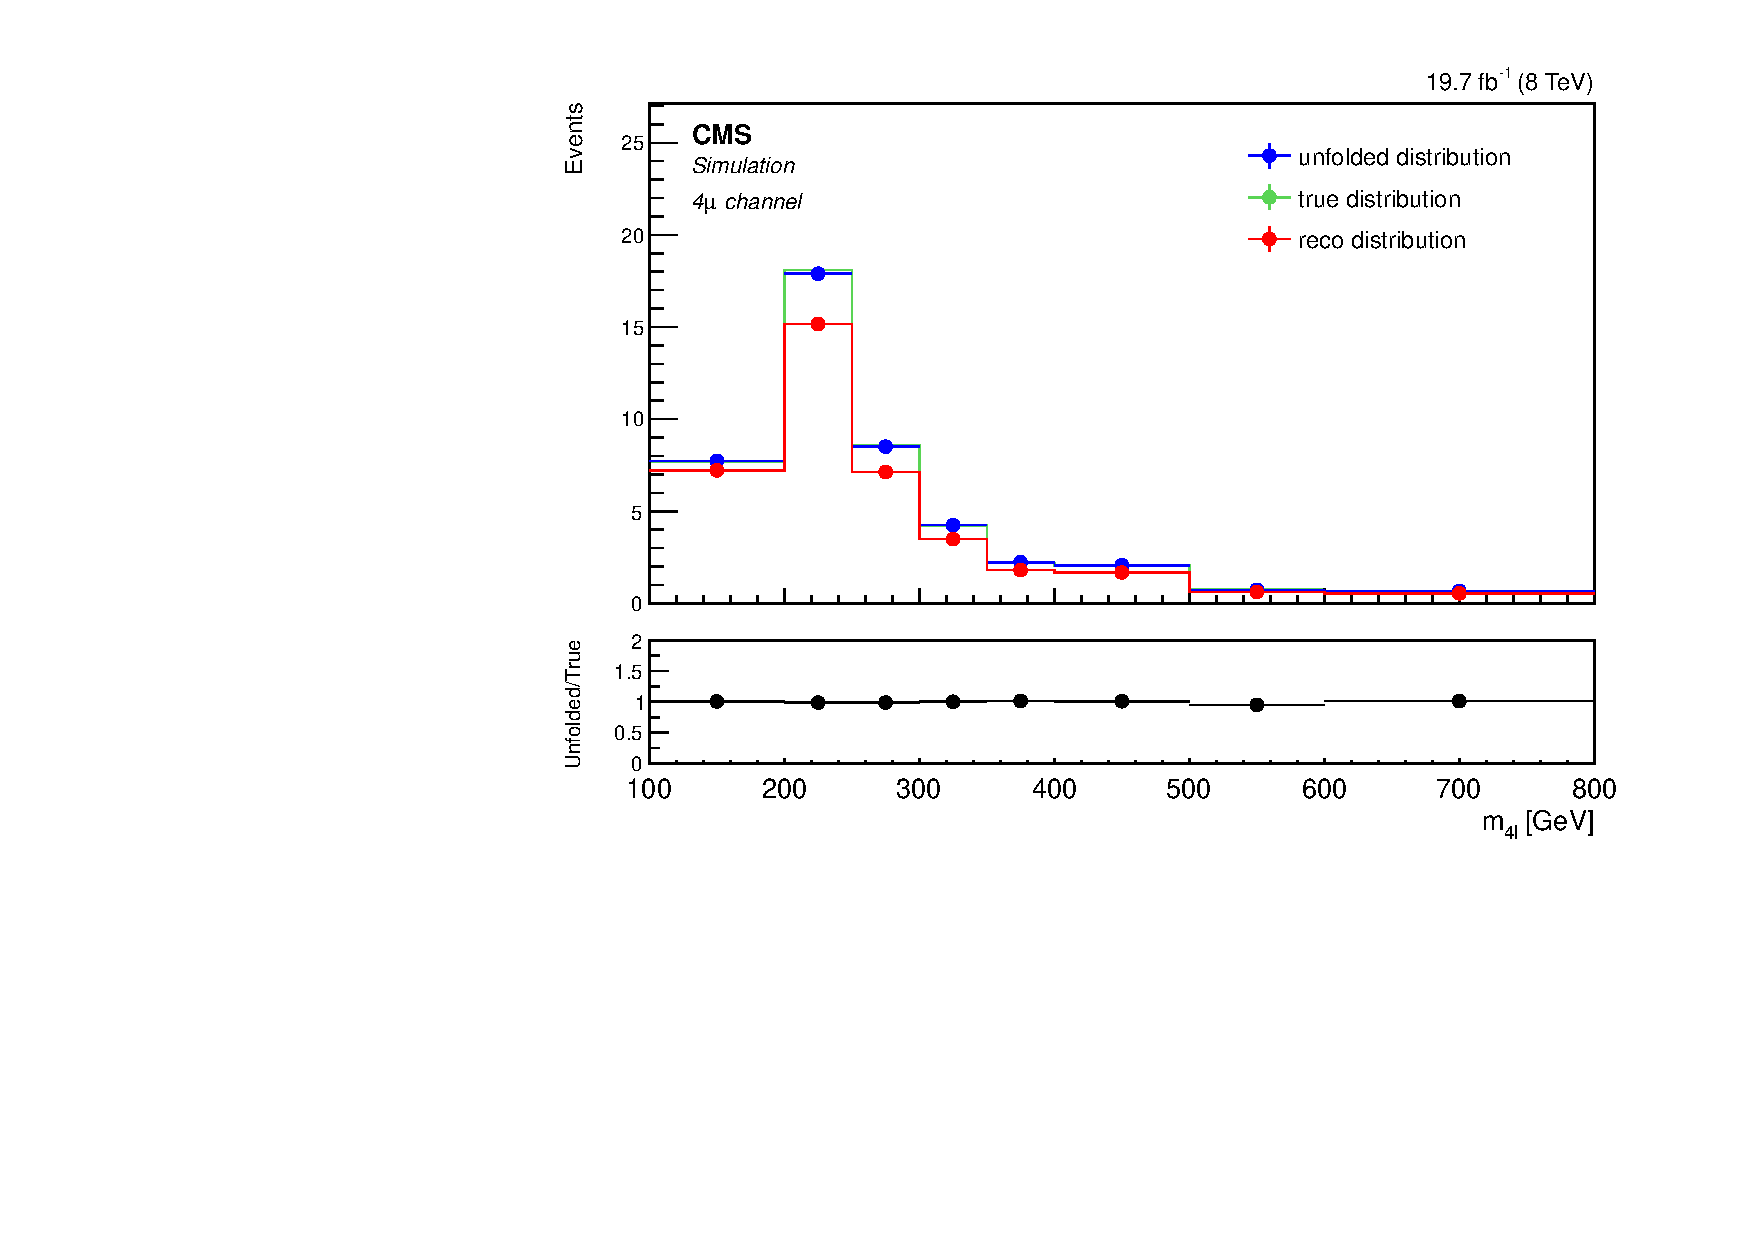
\includegraphics[width=0.8\cmsFigWidth]{Figures/Unfolding/MCTests/Mass_ZZTo4m_PowMatrix_PowDistr_HalfSample_fr}     
 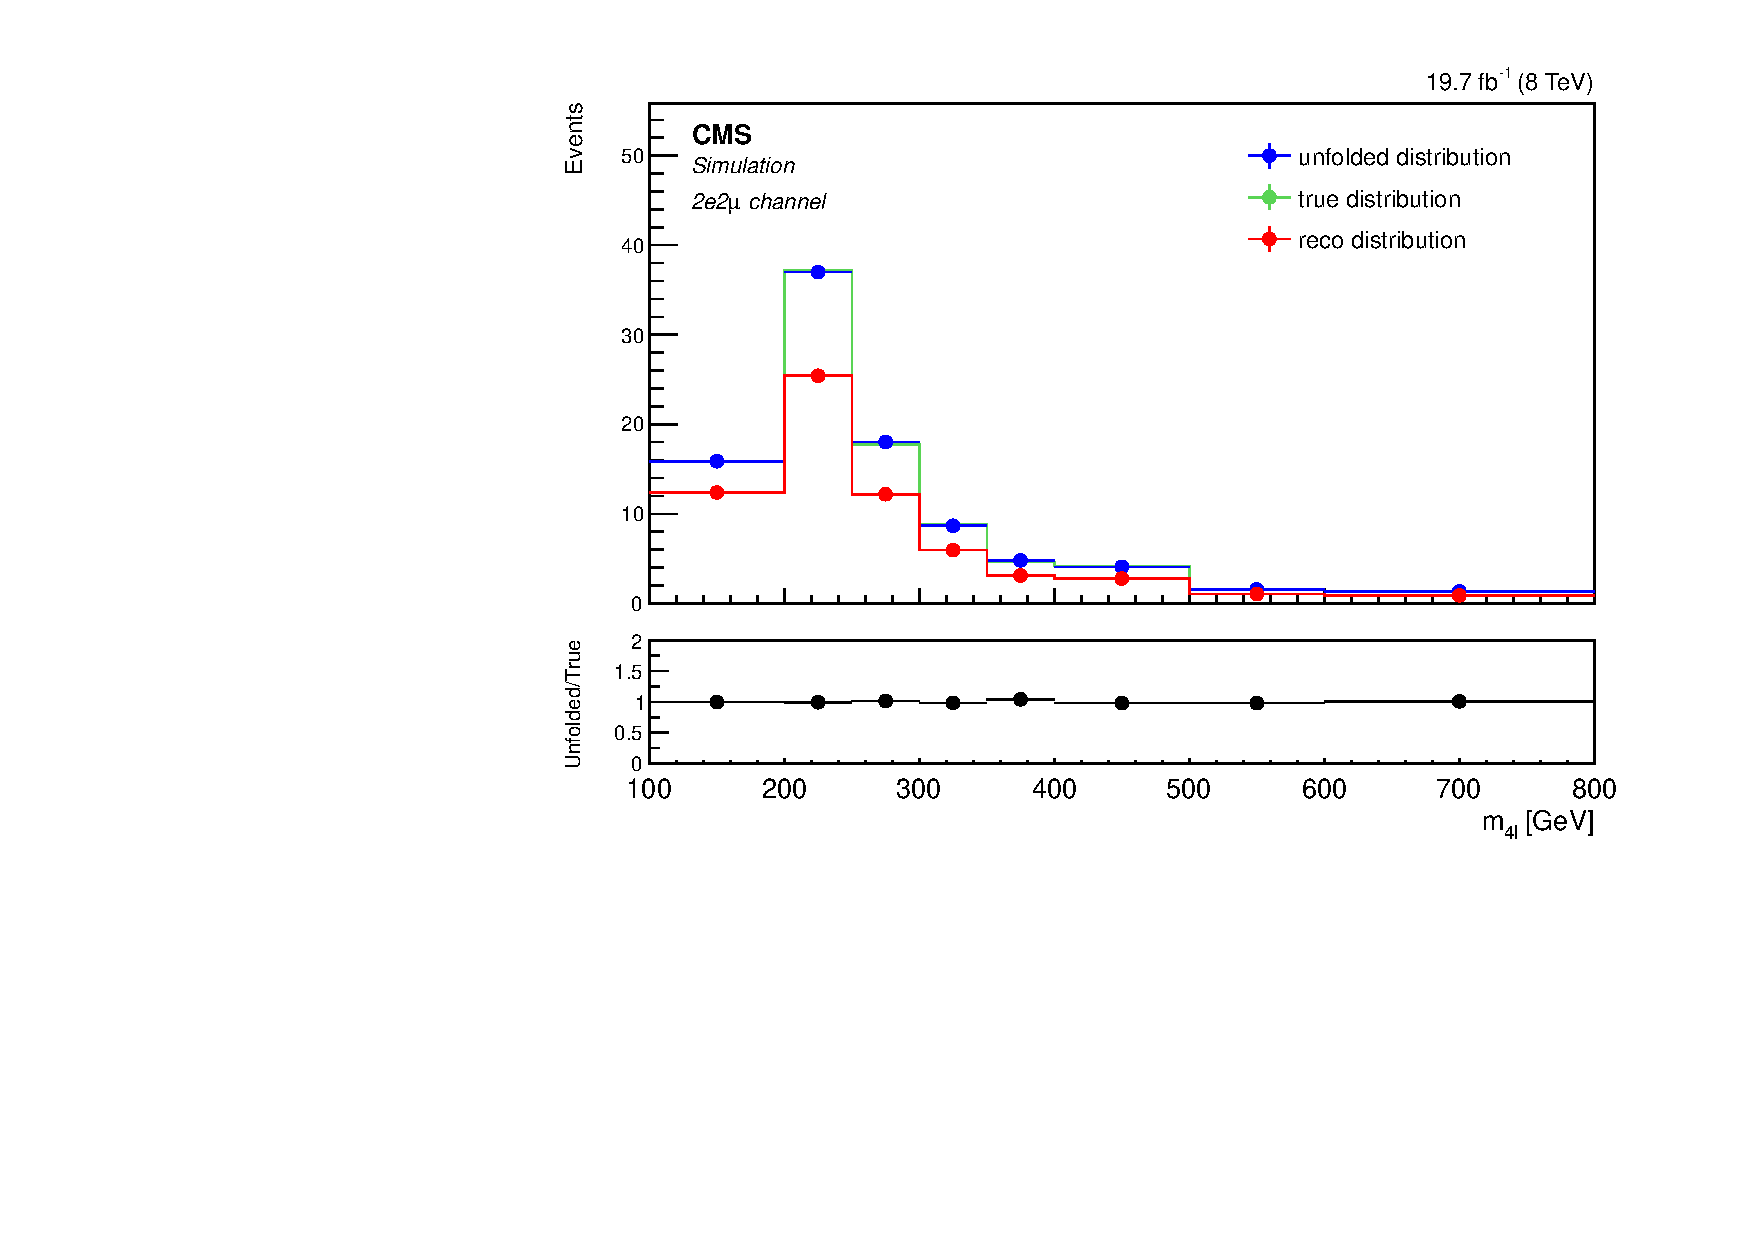
\includegraphics[width=0.8\cmsFigWidth]{Figures/Unfolding/MCTests/Mass_ZZTo2e2m_PowMatrix_PowDistr_HalfSample_fr}        
      \caption{Unfolding tests. From top to bottom: \texttt{MadGraph} matrix applied on \texttt{MadGraph} distribution using the full set, \texttt{Powheg} matrix applied on \texttt{Powheg} distribution using the full set,  \texttt{MadGraph} matrix applied on \texttt{MadGraph} distribution using the two different halves of the total sample set, \texttt{Powheg} matrix applied on \texttt{Powheg} distribution using the two different halves of the total sample set. Results are reported as a function of the 4-lepton mass system for the $4e$ (left), $4\mu$ (center) and $2e2\mu$ (right) final states.}
    \label{fig:MCtest_Mass1}
  \end{center}
\end{figure}

\begin{figure}[hbtp]
  \begin{center}
    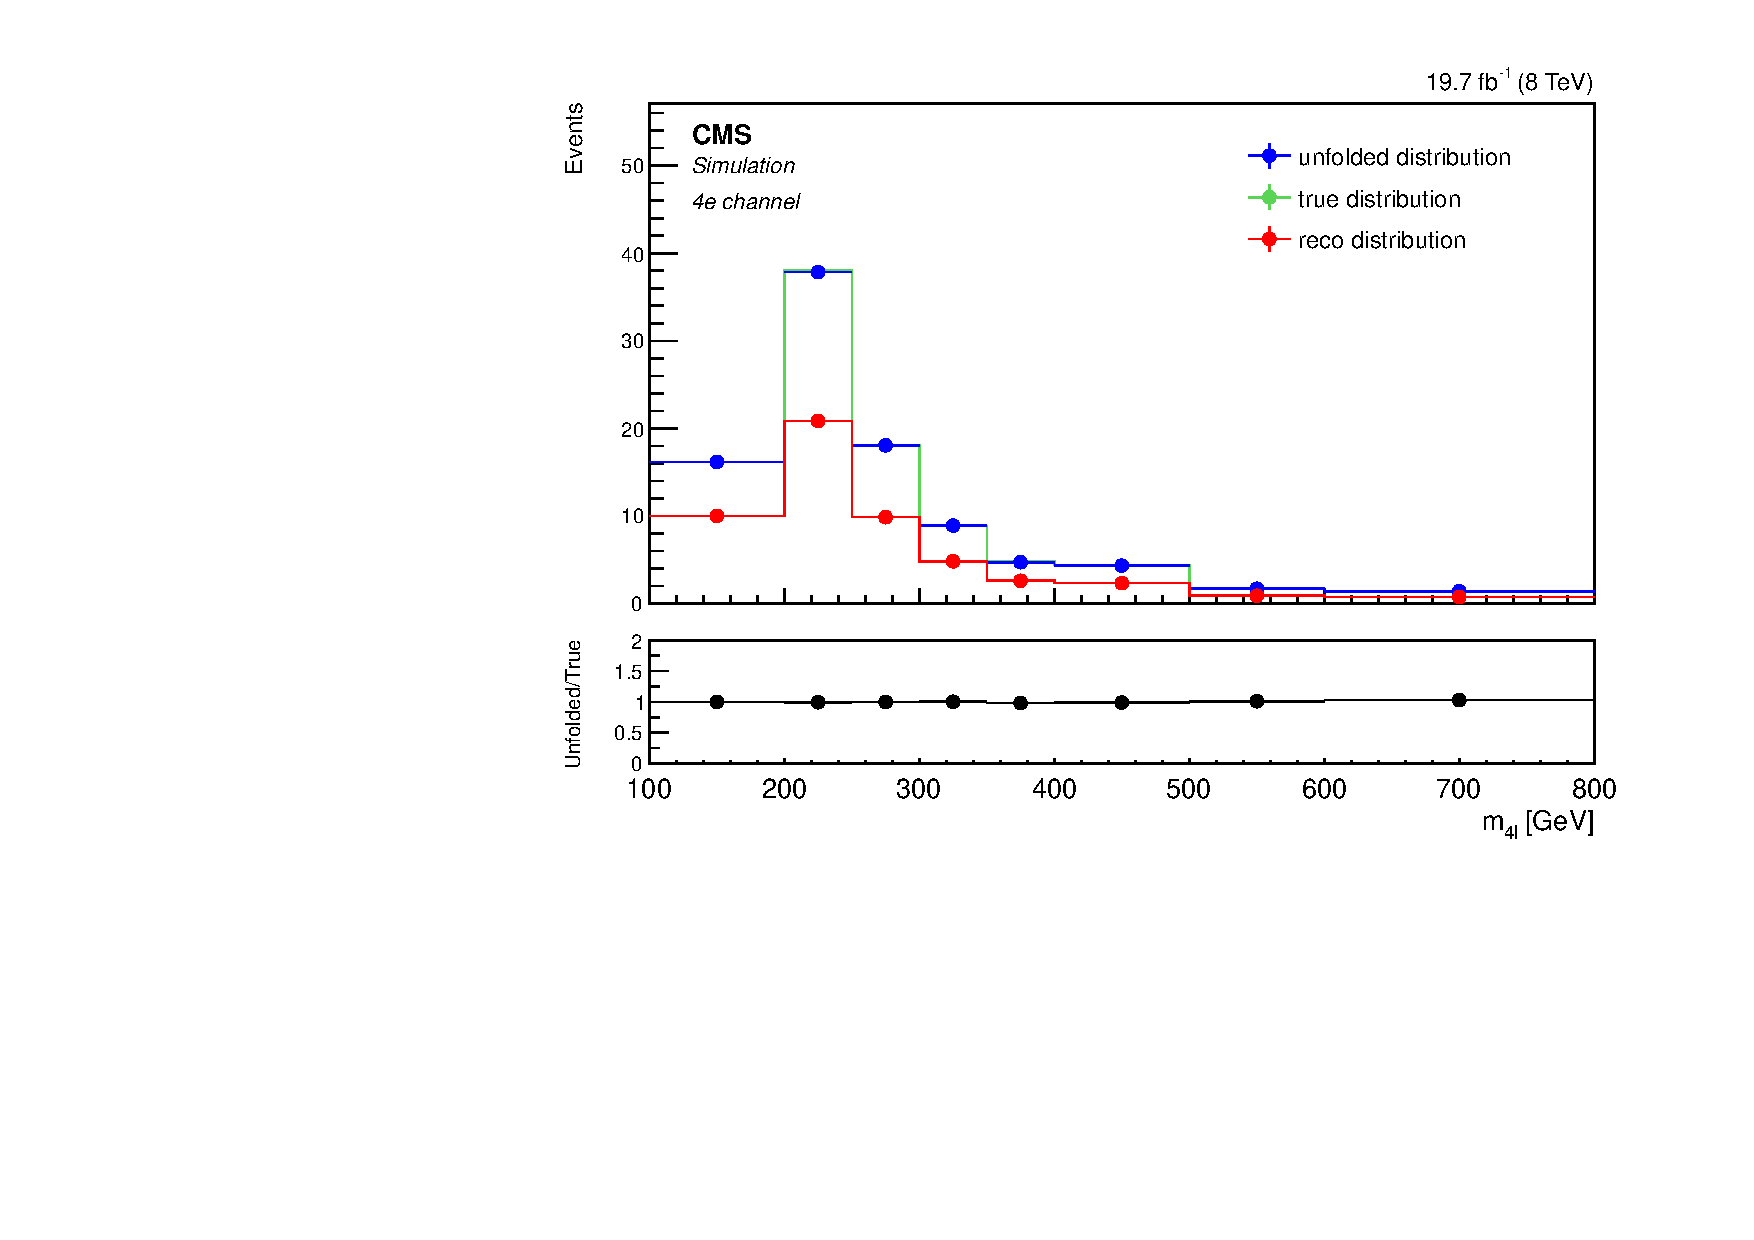
\includegraphics[width=0.8\cmsFigWidth]{Figures/Unfolding/MCTests/Mass_ZZTo4e_MadMatrix_PowDistr_FullSample_fr}     
    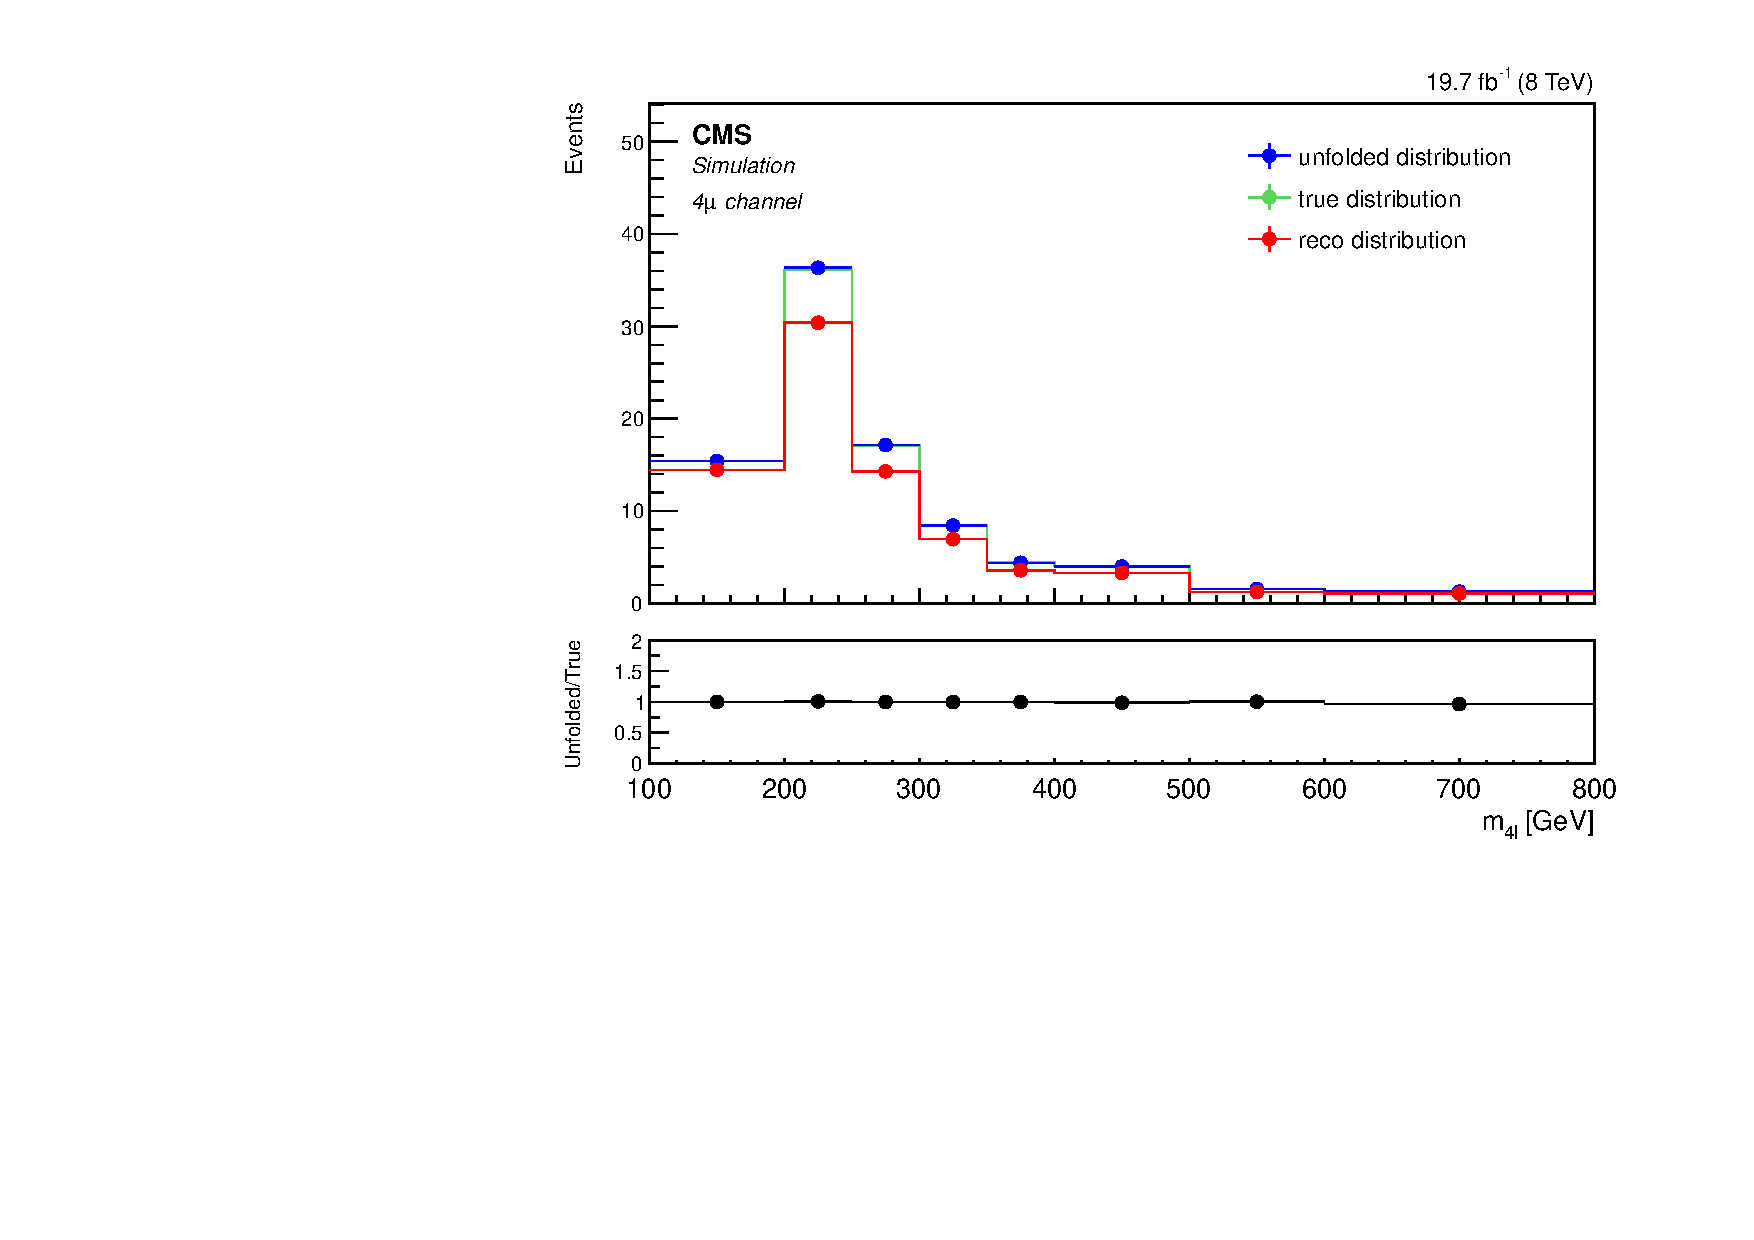
\includegraphics[width=0.8\cmsFigWidth]{Figures/Unfolding/MCTests/Mass_ZZTo4m_MadMatrix_PowDistr_FullSample_fr}     
    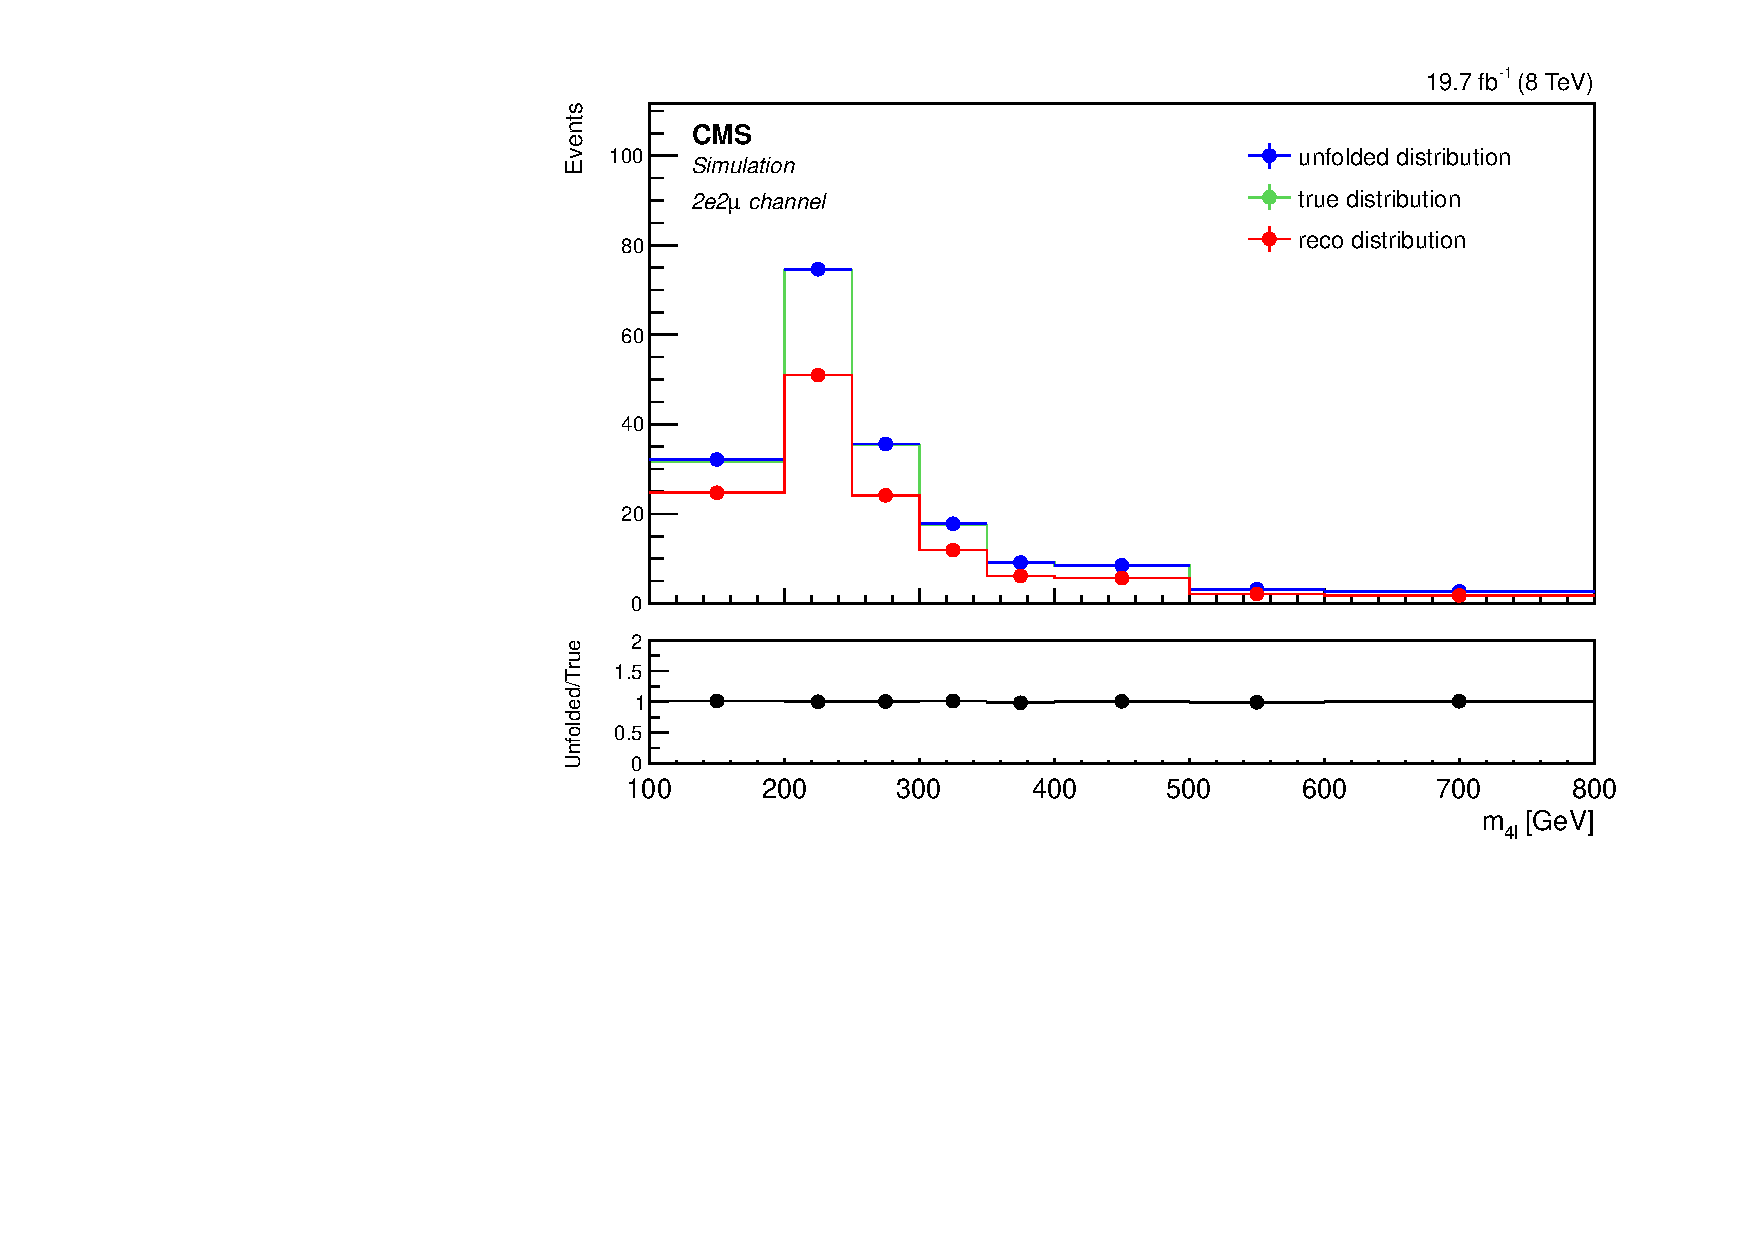
\includegraphics[width=0.8\cmsFigWidth]{Figures/Unfolding/MCTests/Mass_ZZTo2e2m_MadMatrix_PowDistr_FullSample_fr}
     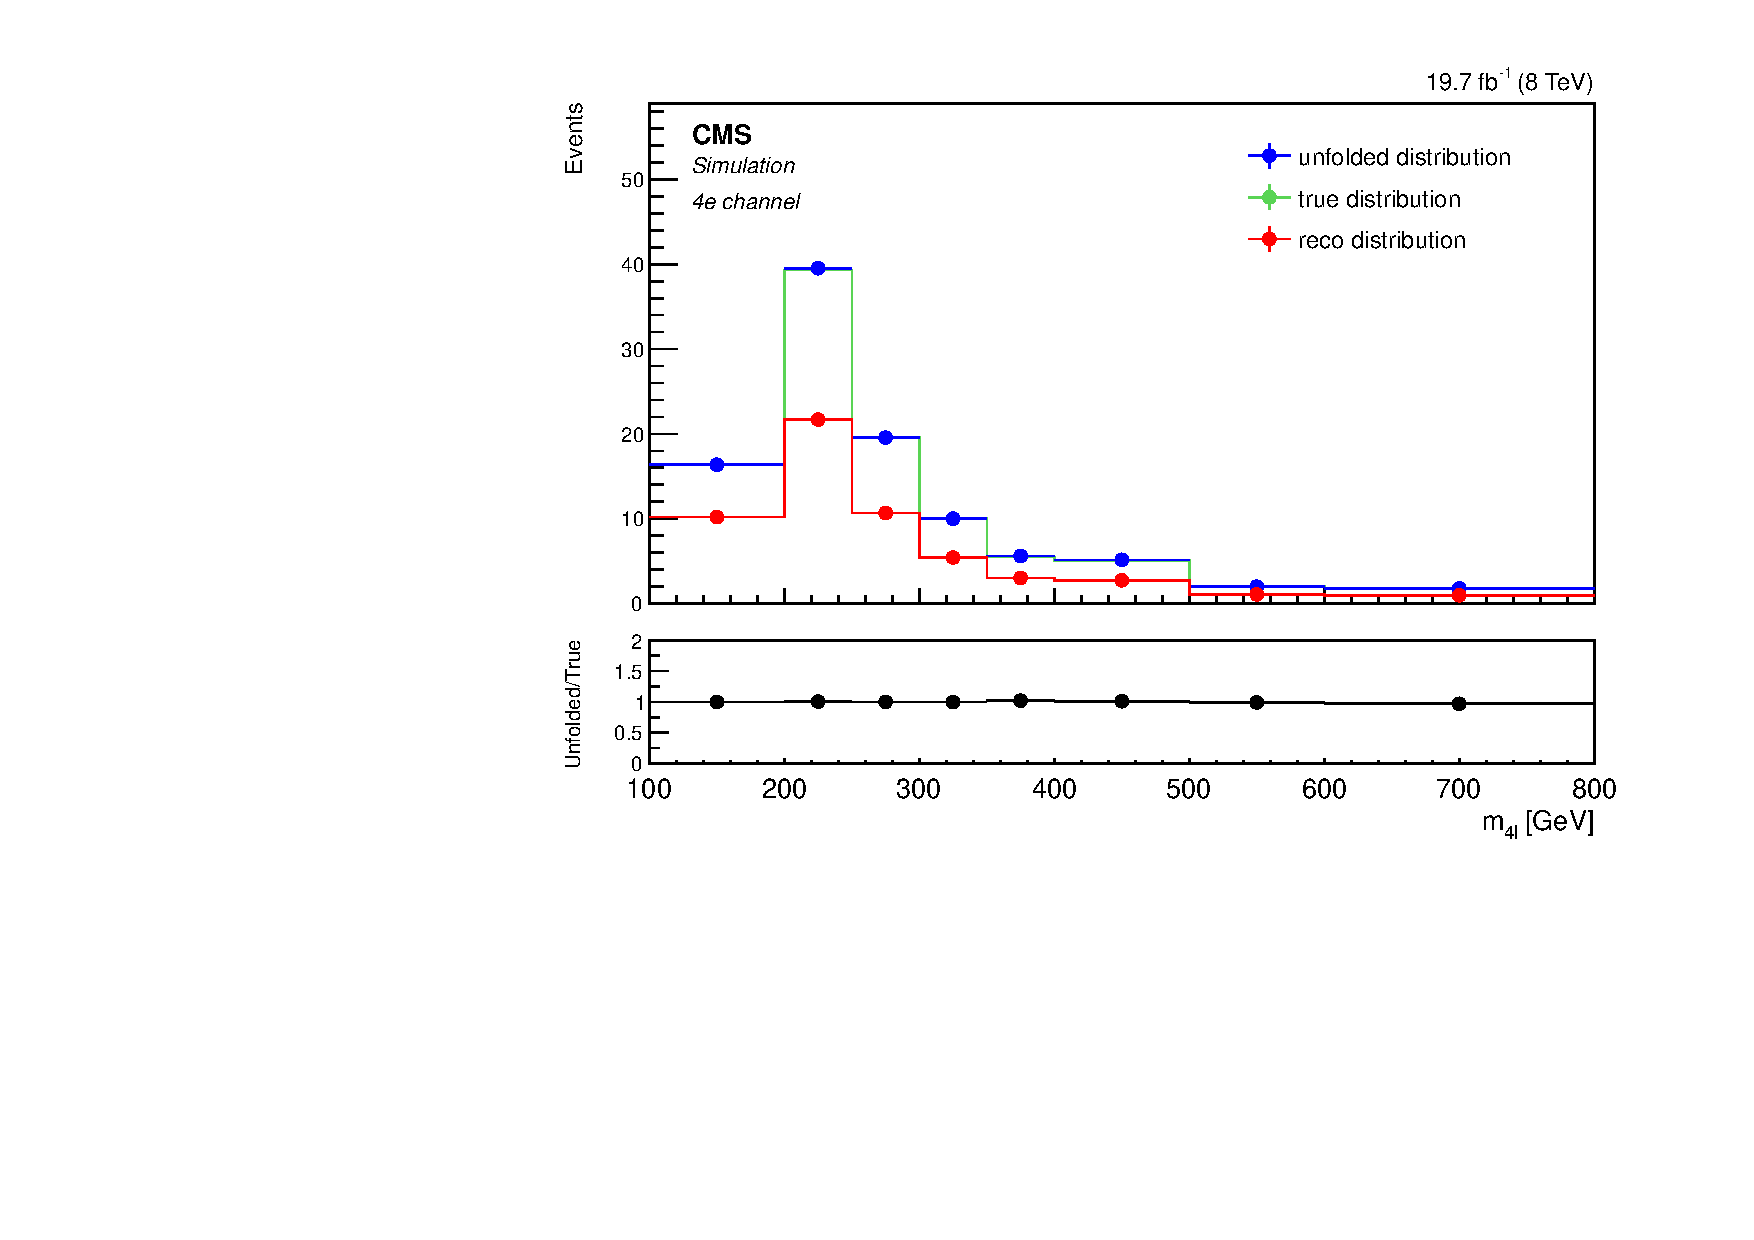
\includegraphics[width=0.8\cmsFigWidth]{Figures/Unfolding/MCTests/Mass_ZZTo4e_PowMatrix_MadDistr_FullSample_fr}     
    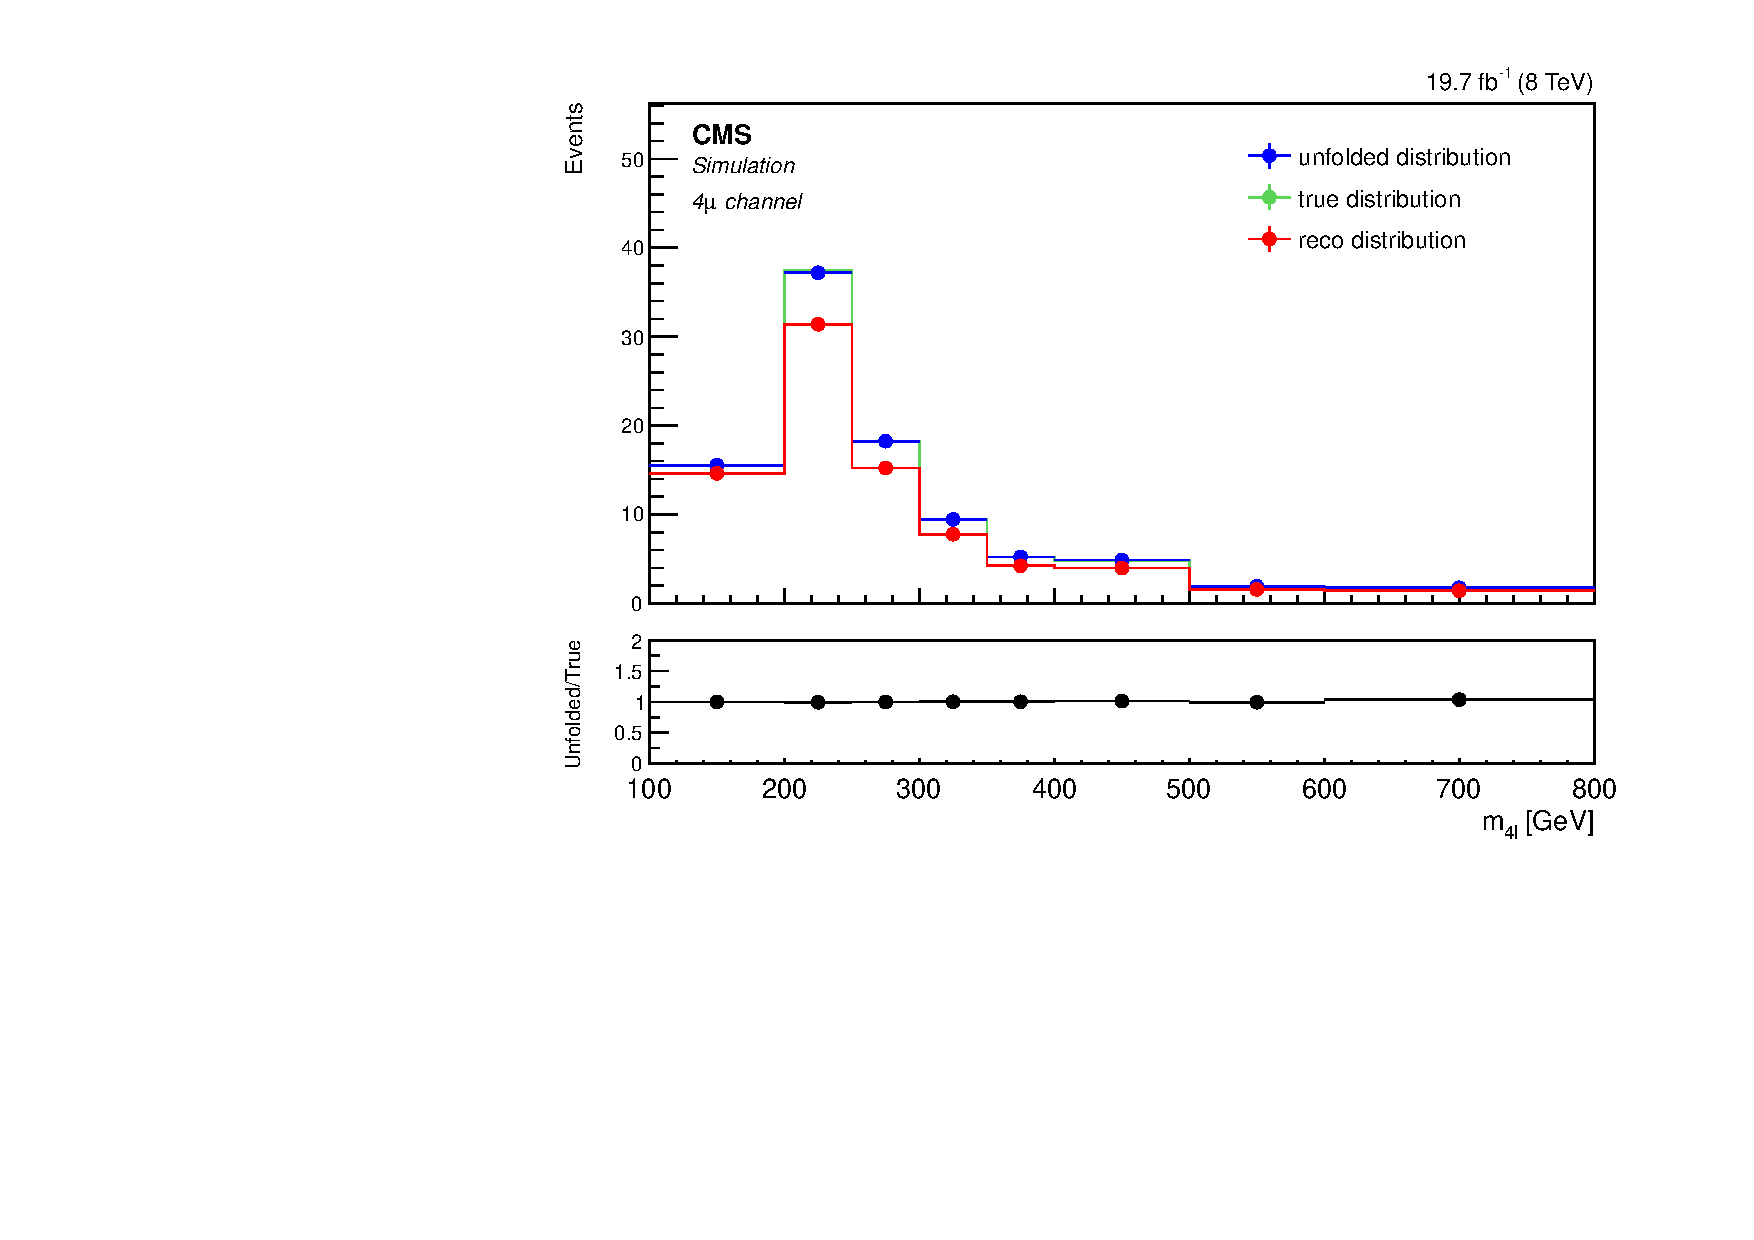
\includegraphics[width=0.8\cmsFigWidth]{Figures/Unfolding/MCTests/Mass_ZZTo4m_PowMatrix_MadDistr_FullSample_fr}     
    \includegraphics[width=0.8\cmsFigWidth]{Figures/Unfolding/MCTests/Mass_ZZTo2e2m_PowMatrix_MadDistr_FullSample_fr}  
 \caption{Unfolding tests. \texttt{MadGraph} matrix applied on \texttt{Powheg} distribution using the full set (top), \texttt{Powheg} matrix applied on \texttt{MadGraph} distribution using the full set (bottom). Results are reported as a function of the 4-lepton mass system for the $4e$ (left), $4\mu$ (center) and $2e2\mu$ (right) final states.}
    \label{fig:MCtest_Mass2}
  \end{center}
\end{figure}
\clearpage
\begin{figure}[hbtp]
  \begin{center}
    \includegraphics[width=0.8\cmsFigWidth]{Figures/Unfolding/MCTests/Jets_ZZTo4e_MadMatrix_MadDistr_FullSample_fr}     
    \includegraphics[width=0.8\cmsFigWidth]{Figures/Unfolding/MCTests/Jets_ZZTo4m_MadMatrix_MadDistr_FullSample_fr}     
    \includegraphics[width=0.8\cmsFigWidth]{Figures/Unfolding/MCTests/Jets_ZZTo2e2m_MadMatrix_MadDistr_FullSample_fr}
     \includegraphics[width=0.8\cmsFigWidth]{Figures/Unfolding/MCTests/Jets_ZZTo4e_PowMatrix_PowDistr_FullSample_fr}     
    \includegraphics[width=0.8\cmsFigWidth]{Figures/Unfolding/MCTests/Jets_ZZTo4m_PowMatrix_PowDistr_FullSample_fr}     
    \includegraphics[width=0.8\cmsFigWidth]{Figures/Unfolding/MCTests/Jets_ZZTo2e2m_PowMatrix_PowDistr_FullSample_fr}      
    \includegraphics[width=0.8\cmsFigWidth]{Figures/Unfolding/MCTests/Jets_ZZTo4e_MadMatrix_MadDistr_HalfSample_fr}     
    \includegraphics[width=0.8\cmsFigWidth]{Figures/Unfolding/MCTests/Jets_ZZTo4m_MadMatrix_MadDistr_HalfSample_fr}     
    \includegraphics[width=0.8\cmsFigWidth]{Figures/Unfolding/MCTests/Jets_ZZTo2e2m_MadMatrix_MadDistr_HalfSample_fr}     
    \includegraphics[width=0.8\cmsFigWidth]{Figures/Unfolding/MCTests/Jets_ZZTo4e_PowMatrix_PowDistr_HalfSample_fr}     
    \includegraphics[width=0.8\cmsFigWidth]{Figures/Unfolding/MCTests/Jets_ZZTo4m_PowMatrix_PowDistr_HalfSample_fr}     
 \includegraphics[width=0.8\cmsFigWidth]{Figures/Unfolding/MCTests/Jets_ZZTo2e2m_PowMatrix_PowDistr_HalfSample_fr}        
      \caption{Unfolding tests. From top to bottom: \texttt{MadGraph} matrix applied on \texttt{MadGraph} distribution using the full set, \texttt{Powheg} matrix applied on \texttt{Powheg} distribution using the full set,  \texttt{MadGraph} matrix applied on \texttt{MadGraph} distribution using the two different halves of the total sample set, \texttt{Powheg} matrix applied on \texttt{Powheg} distribution using the two different halves of the total sample set. Results are reported as a function of the number of jets for the $4e$ (left), $4\mu$ (center) and $2e2\mu$ (right) final states.}
    \label{fig:MCtest_Jets1}
  \end{center}
\end{figure}

\begin{figure}[hbtp]
  \begin{center}
    \includegraphics[width=0.8\cmsFigWidth]{Figures/Unfolding/MCTests/Jets_ZZTo4e_MadMatrix_PowDistr_FullSample_fr}     
    \includegraphics[width=0.8\cmsFigWidth]{Figures/Unfolding/MCTests/Jets_ZZTo4m_MadMatrix_PowDistr_FullSample_fr}     
    \includegraphics[width=0.8\cmsFigWidth]{Figures/Unfolding/MCTests/Jets_ZZTo2e2m_MadMatrix_PowDistr_FullSample_fr}
     \includegraphics[width=0.8\cmsFigWidth]{Figures/Unfolding/MCTests/Jets_ZZTo4e_PowMatrix_MadDistr_FullSample_fr}     
    \includegraphics[width=0.8\cmsFigWidth]{Figures/Unfolding/MCTests/Jets_ZZTo4m_PowMatrix_MadDistr_FullSample_fr}     
    \includegraphics[width=0.8\cmsFigWidth]{Figures/Unfolding/MCTests/Jets_ZZTo2e2m_PowMatrix_MadDistr_FullSample_fr}  
 \caption{Unfolding tests. \texttt{MadGraph} matrix applied on \texttt{Powheg} distribution using the full set (top), \texttt{Powheg} matrix applied on \texttt{MadGraph} distribution using the full set (bottom). Results are reported as a function of the number of jets for the $4e$ (left), $4\mu$ (center) and $2e2\mu$ (right) final states.}
    \label{fig:MCtest_Jets2}
  \end{center}
\end{figure}
\clearpage
\begin{figure}[hbtp]
  \begin{center}
    \includegraphics[width=0.8\cmsFigWidth]{Figures/Unfolding/MCTests/CentralJets_ZZTo4e_MadMatrix_MadDistr_FullSample_fr}     
    \includegraphics[width=0.8\cmsFigWidth]{Figures/Unfolding/MCTests/CentralJets_ZZTo4m_MadMatrix_MadDistr_FullSample_fr}     
    \includegraphics[width=0.8\cmsFigWidth]{Figures/Unfolding/MCTests/CentralJets_ZZTo2e2m_MadMatrix_MadDistr_FullSample_fr}
     \includegraphics[width=0.8\cmsFigWidth]{Figures/Unfolding/MCTests/CentralJets_ZZTo4e_PowMatrix_PowDistr_FullSample_fr}     
    \includegraphics[width=0.8\cmsFigWidth]{Figures/Unfolding/MCTests/CentralJets_ZZTo4m_PowMatrix_PowDistr_FullSample_fr}     
    \includegraphics[width=0.8\cmsFigWidth]{Figures/Unfolding/MCTests/CentralJets_ZZTo2e2m_PowMatrix_PowDistr_FullSample_fr}      
    \includegraphics[width=0.8\cmsFigWidth]{Figures/Unfolding/MCTests/CentralJets_ZZTo4e_MadMatrix_MadDistr_HalfSample_fr}     
    \includegraphics[width=0.8\cmsFigWidth]{Figures/Unfolding/MCTests/CentralJets_ZZTo4m_MadMatrix_MadDistr_HalfSample_fr}     
    \includegraphics[width=0.8\cmsFigWidth]{Figures/Unfolding/MCTests/CentralJets_ZZTo2e2m_MadMatrix_MadDistr_HalfSample_fr}     
    \includegraphics[width=0.8\cmsFigWidth]{Figures/Unfolding/MCTests/CentralJets_ZZTo4e_PowMatrix_PowDistr_HalfSample_fr}     
    \includegraphics[width=0.8\cmsFigWidth]{Figures/Unfolding/MCTests/CentralJets_ZZTo4m_PowMatrix_PowDistr_HalfSample_fr}     
 \includegraphics[width=0.8\cmsFigWidth]{Figures/Unfolding/MCTests/CentralJets_ZZTo2e2m_PowMatrix_PowDistr_HalfSample_fr}        
      \caption{Unfolding tests. From top to bottom: \texttt{MadGraph} matrix applied on \texttt{MadGraph} distribution using the full set, \texttt{Powheg} matrix applied on \texttt{Powheg} distribution using the full set,  \texttt{MadGraph} matrix applied on \texttt{MadGraph} distribution using the two different halves of the total sample set, \texttt{Powheg} matrix applied on \texttt{Powheg} distribution using the two different halves of the total sample set. Results are reported as a function of the number of central jets for the $4e$ (left), $4\mu$ (center) and $2e2\mu$ (right) final states.}
    \label{fig:MCtest_CentralJets1}
  \end{center}
\end{figure}

\begin{figure}[hbtp]
  \begin{center}
    \includegraphics[width=0.8\cmsFigWidth]{Figures/Unfolding/MCTests/CentralJets_ZZTo4e_MadMatrix_PowDistr_FullSample_fr}     
    \includegraphics[width=0.8\cmsFigWidth]{Figures/Unfolding/MCTests/CentralJets_ZZTo4m_MadMatrix_PowDistr_FullSample_fr}     
    \includegraphics[width=0.8\cmsFigWidth]{Figures/Unfolding/MCTests/CentralJets_ZZTo2e2m_MadMatrix_PowDistr_FullSample_fr}
     \includegraphics[width=0.8\cmsFigWidth]{Figures/Unfolding/MCTests/CentralJets_ZZTo4e_PowMatrix_MadDistr_FullSample_fr}     
    \includegraphics[width=0.8\cmsFigWidth]{Figures/Unfolding/MCTests/CentralJets_ZZTo4m_PowMatrix_MadDistr_FullSample_fr}     
    \includegraphics[width=0.8\cmsFigWidth]{Figures/Unfolding/MCTests/CentralJets_ZZTo2e2m_PowMatrix_MadDistr_FullSample_fr}  
 \caption{Unfolding tests. \texttt{MadGraph} matrix applied on \texttt{Powheg} distribution using the full set (top), \texttt{Powheg} matrix applied on \texttt{MadGraph} distribution using the full set (bottom). Results are reported as a function of the number of central jets for the $4e$ (left), $4\mu$ (center) and $2e2\mu$ (right) final states.}
    \label{fig:MCtest_CentralJets2}
  \end{center}
\end{figure}
\clearpage 
\begin{figure}[hbtp]
  \begin{center}
    \includegraphics[width=0.8\cmsFigWidth]{Figures/Unfolding/MCTests/Mjj_ZZTo4e_MadMatrix_MadDistr_FullSample_fr}     
    \includegraphics[width=0.8\cmsFigWidth]{Figures/Unfolding/MCTests/Mjj_ZZTo4m_MadMatrix_MadDistr_FullSample_fr}     
    \includegraphics[width=0.8\cmsFigWidth]{Figures/Unfolding/MCTests/Mjj_ZZTo2e2m_MadMatrix_MadDistr_FullSample_fr}
     \includegraphics[width=0.8\cmsFigWidth]{Figures/Unfolding/MCTests/Mjj_ZZTo4e_PowMatrix_PowDistr_FullSample_fr}     
    \includegraphics[width=0.8\cmsFigWidth]{Figures/Unfolding/MCTests/Mjj_ZZTo4m_PowMatrix_PowDistr_FullSample_fr}     
    \includegraphics[width=0.8\cmsFigWidth]{Figures/Unfolding/MCTests/Mjj_ZZTo2e2m_PowMatrix_PowDistr_FullSample_fr}      
    \includegraphics[width=0.8\cmsFigWidth]{Figures/Unfolding/MCTests/Mjj_ZZTo4e_MadMatrix_MadDistr_HalfSample_fr}     
    \includegraphics[width=0.8\cmsFigWidth]{Figures/Unfolding/MCTests/Mjj_ZZTo4m_MadMatrix_MadDistr_HalfSample_fr}     
    \includegraphics[width=0.8\cmsFigWidth]{Figures/Unfolding/MCTests/Mjj_ZZTo2e2m_MadMatrix_MadDistr_HalfSample_fr}     
    \includegraphics[width=0.8\cmsFigWidth]{Figures/Unfolding/MCTests/Mjj_ZZTo4e_PowMatrix_PowDistr_HalfSample_fr}     
    \includegraphics[width=0.8\cmsFigWidth]{Figures/Unfolding/MCTests/Mjj_ZZTo4m_PowMatrix_PowDistr_HalfSample_fr}     
 \includegraphics[width=0.8\cmsFigWidth]{Figures/Unfolding/MCTests/Mjj_ZZTo2e2m_PowMatrix_PowDistr_HalfSample_fr}        
      \caption{Unfolding tests. From top to bottom: \texttt{MadGraph} matrix applied on \texttt{MadGraph} distribution using the full set, \texttt{Powheg} matrix applied on \texttt{Powheg} distribution using the full set,  \texttt{MadGraph} matrix applied on \texttt{MadGraph} distribution using the two different halves of the total sample set, \texttt{Powheg} matrix applied on \texttt{Powheg} distribution using the two different halves of the total sample set. Results are reported as a function of $m_{jj}$ for the $4e$ (left), $4\mu$ (center) and $2e2\mu$ (right) final states.}
    \label{fig:MCtest_Mjj1}
  \end{center}
\end{figure}

\begin{figure}[hbtp]
  \begin{center}
    \includegraphics[width=0.8\cmsFigWidth]{Figures/Unfolding/MCTests/Mjj_ZZTo4e_MadMatrix_PowDistr_FullSample_fr}     
    \includegraphics[width=0.8\cmsFigWidth]{Figures/Unfolding/MCTests/Mjj_ZZTo4m_MadMatrix_PowDistr_FullSample_fr}     
    \includegraphics[width=0.8\cmsFigWidth]{Figures/Unfolding/MCTests/Mjj_ZZTo2e2m_MadMatrix_PowDistr_FullSample_fr}
     \includegraphics[width=0.8\cmsFigWidth]{Figures/Unfolding/MCTests/Mjj_ZZTo4e_PowMatrix_MadDistr_FullSample_fr}     
    \includegraphics[width=0.8\cmsFigWidth]{Figures/Unfolding/MCTests/Mjj_ZZTo4m_PowMatrix_MadDistr_FullSample_fr}     
    \includegraphics[width=0.8\cmsFigWidth]{Figures/Unfolding/MCTests/Mjj_ZZTo2e2m_PowMatrix_MadDistr_FullSample_fr}  
 \caption{Unfolding tests. \texttt{MadGraph} matrix applied on \texttt{Powheg} distribution using the full set (top), \texttt{Powheg} matrix applied on \texttt{MadGraph} distribution using the full set (bottom). Results are reported as a function of $m_{jj}$ for the $4e$ (left), $4\mu$ (center) and $2e2\mu$ (right) final states.}
    \label{fig:MCtest_Mjj2}
  \end{center}
\end{figure}
\clearpage 
\begin{figure}[hbtp]
  \begin{center}
    \includegraphics[width=0.8\cmsFigWidth]{Figures/Unfolding/MCTests/CentralMjj_ZZTo4e_MadMatrix_MadDistr_FullSample_fr}     
    \includegraphics[width=0.8\cmsFigWidth]{Figures/Unfolding/MCTests/CentralMjj_ZZTo4m_MadMatrix_MadDistr_FullSample_fr}     
    \includegraphics[width=0.8\cmsFigWidth]{Figures/Unfolding/MCTests/CentralMjj_ZZTo2e2m_MadMatrix_MadDistr_FullSample_fr}
     \includegraphics[width=0.8\cmsFigWidth]{Figures/Unfolding/MCTests/CentralMjj_ZZTo4e_PowMatrix_PowDistr_FullSample_fr}     
    \includegraphics[width=0.8\cmsFigWidth]{Figures/Unfolding/MCTests/CentralMjj_ZZTo4m_PowMatrix_PowDistr_FullSample_fr}     
    \includegraphics[width=0.8\cmsFigWidth]{Figures/Unfolding/MCTests/CentralMjj_ZZTo2e2m_PowMatrix_PowDistr_FullSample_fr}      
    \includegraphics[width=0.8\cmsFigWidth]{Figures/Unfolding/MCTests/CentralMjj_ZZTo4e_MadMatrix_MadDistr_HalfSample_fr}     
    \includegraphics[width=0.8\cmsFigWidth]{Figures/Unfolding/MCTests/CentralMjj_ZZTo4m_MadMatrix_MadDistr_HalfSample_fr}     
    \includegraphics[width=0.8\cmsFigWidth]{Figures/Unfolding/MCTests/CentralMjj_ZZTo2e2m_MadMatrix_MadDistr_HalfSample_fr}     
    \includegraphics[width=0.8\cmsFigWidth]{Figures/Unfolding/MCTests/CentralMjj_ZZTo4e_PowMatrix_PowDistr_HalfSample_fr}     
    \includegraphics[width=0.8\cmsFigWidth]{Figures/Unfolding/MCTests/CentralMjj_ZZTo4m_PowMatrix_PowDistr_HalfSample_fr}     
 \includegraphics[width=0.8\cmsFigWidth]{Figures/Unfolding/MCTests/CentralMjj_ZZTo2e2m_PowMatrix_PowDistr_HalfSample_fr}        
      \caption{Unfolding tests. From top to bottom: \texttt{MadGraph} matrix applied on \texttt{MadGraph} distribution using the full set, \texttt{Powheg} matrix applied on \texttt{Powheg} distribution using the full set,  \texttt{MadGraph} matrix applied on \texttt{MadGraph} distribution using the two different halves of the total sample set, \texttt{Powheg} matrix applied on \texttt{Powheg} distribution using the two different halves of the total sample set. Results are reported as a function of $m_{jj}$ (with $|\eta^{jet}|<2.4$) for the $4e$ (left), $4\mu$ (center) and $2e2\mu$ (right) final states.}
    \label{fig:MCtest_CentralMjj1}
  \end{center}
\end{figure}

\begin{figure}[hbtp]
  \begin{center}
    \includegraphics[width=0.8\cmsFigWidth]{Figures/Unfolding/MCTests/CentralMjj_ZZTo4e_MadMatrix_PowDistr_FullSample_fr}     
    \includegraphics[width=0.8\cmsFigWidth]{Figures/Unfolding/MCTests/CentralMjj_ZZTo4m_MadMatrix_PowDistr_FullSample_fr}     
    \includegraphics[width=0.8\cmsFigWidth]{Figures/Unfolding/MCTests/CentralMjj_ZZTo2e2m_MadMatrix_PowDistr_FullSample_fr}
     \includegraphics[width=0.8\cmsFigWidth]{Figures/Unfolding/MCTests/CentralMjj_ZZTo4e_PowMatrix_MadDistr_FullSample_fr}     
    \includegraphics[width=0.8\cmsFigWidth]{Figures/Unfolding/MCTests/CentralMjj_ZZTo4m_PowMatrix_MadDistr_FullSample_fr}     
    \includegraphics[width=0.8\cmsFigWidth]{Figures/Unfolding/MCTests/CentralMjj_ZZTo2e2m_PowMatrix_MadDistr_FullSample_fr}  
 \caption{Unfolding tests. \texttt{MadGraph} matrix applied on \texttt{Powheg} distribution using the full set (top), \texttt{Powheg} matrix applied on \texttt{MadGraph} distribution using the full set (bottom). Results are reported as a function of $m_{jj}$ (with $|\eta^{jet}|<2.4$) for the $4e$ (left), $4\mu$ (center) and $2e2\mu$ (right) final states.}
    \label{fig:MCtest_CentralMjj2}
  \end{center}
\end{figure}
\clearpage 
\begin{figure}[hbtp]
  \begin{center}
    \includegraphics[width=0.8\cmsFigWidth]{Figures/Unfolding/MCTests/Deta_ZZTo4e_MadMatrix_MadDistr_FullSample_fr}     
    \includegraphics[width=0.8\cmsFigWidth]{Figures/Unfolding/MCTests/Deta_ZZTo4m_MadMatrix_MadDistr_FullSample_fr}     
    \includegraphics[width=0.8\cmsFigWidth]{Figures/Unfolding/MCTests/Deta_ZZTo2e2m_MadMatrix_MadDistr_FullSample_fr}
     \includegraphics[width=0.8\cmsFigWidth]{Figures/Unfolding/MCTests/Deta_ZZTo4e_PowMatrix_PowDistr_FullSample_fr}     
    \includegraphics[width=0.8\cmsFigWidth]{Figures/Unfolding/MCTests/Deta_ZZTo4m_PowMatrix_PowDistr_FullSample_fr}     
    \includegraphics[width=0.8\cmsFigWidth]{Figures/Unfolding/MCTests/Deta_ZZTo2e2m_PowMatrix_PowDistr_FullSample_fr}      
    \includegraphics[width=0.8\cmsFigWidth]{Figures/Unfolding/MCTests/Deta_ZZTo4e_MadMatrix_MadDistr_HalfSample_fr}     
    \includegraphics[width=0.8\cmsFigWidth]{Figures/Unfolding/MCTests/Deta_ZZTo4m_MadMatrix_MadDistr_HalfSample_fr}     
    \includegraphics[width=0.8\cmsFigWidth]{Figures/Unfolding/MCTests/Deta_ZZTo2e2m_MadMatrix_MadDistr_HalfSample_fr}     
    \includegraphics[width=0.8\cmsFigWidth]{Figures/Unfolding/MCTests/Deta_ZZTo4e_PowMatrix_PowDistr_HalfSample_fr}     
    \includegraphics[width=0.8\cmsFigWidth]{Figures/Unfolding/MCTests/Deta_ZZTo4m_PowMatrix_PowDistr_HalfSample_fr}     
 \includegraphics[width=0.8\cmsFigWidth]{Figures/Unfolding/MCTests/Deta_ZZTo2e2m_PowMatrix_PowDistr_HalfSample_fr}        
      \caption{Unfolding tests. From top to bottom: \texttt{MadGraph} matrix applied on \texttt{MadGraph} distribution using the full set, \texttt{Powheg} matrix applied on \texttt{Powheg} distribution using the full set,  \texttt{MadGraph} matrix applied on \texttt{MadGraph} distribution using the two different halves of the total sample set, \texttt{Powheg} matrix applied on \texttt{Powheg} distribution using the two different halves of the total sample set. Results are reported as a function of $\Delta\eta_{jj}$ for the $4e$ (left), $4\mu$ (center) and $2e2\mu$ (right) final states.}
    \label{fig:MCtest_Deta1}
  \end{center}
\end{figure}

\begin{figure}[hbtp]
  \begin{center}
    \includegraphics[width=0.8\cmsFigWidth]{Figures/Unfolding/MCTests/Deta_ZZTo4e_MadMatrix_PowDistr_FullSample_fr}     
    \includegraphics[width=0.8\cmsFigWidth]{Figures/Unfolding/MCTests/Deta_ZZTo4m_MadMatrix_PowDistr_FullSample_fr}     
    \includegraphics[width=0.8\cmsFigWidth]{Figures/Unfolding/MCTests/Deta_ZZTo2e2m_MadMatrix_PowDistr_FullSample_fr}
     \includegraphics[width=0.8\cmsFigWidth]{Figures/Unfolding/MCTests/Deta_ZZTo4e_PowMatrix_MadDistr_FullSample_fr}     
    \includegraphics[width=0.8\cmsFigWidth]{Figures/Unfolding/MCTests/Deta_ZZTo4m_PowMatrix_MadDistr_FullSample_fr}     
    \includegraphics[width=0.8\cmsFigWidth]{Figures/Unfolding/MCTests/Deta_ZZTo2e2m_PowMatrix_MadDistr_FullSample_fr}  
 \caption{Unfolding tests. \texttt{MadGraph} matrix applied on \texttt{Powheg} distribution using the full set (top), \texttt{Powheg} matrix applied on \texttt{MadGraph} distribution using the full set (bottom). Results are reported as a function of $\Delta\eta_{jj}$ for the $4e$ (left), $4\mu$ (center) and $2e2\mu$ (right) final states.}
    \label{fig:MCtest_Deta2}
  \end{center}
\end{figure}
\clearpage 
\begin{figure}[hbtp]
  \begin{center}
    \includegraphics[width=0.8\cmsFigWidth]{Figures/Unfolding/MCTests/CentralDeta_ZZTo4e_MadMatrix_MadDistr_FullSample_fr}     
    \includegraphics[width=0.8\cmsFigWidth]{Figures/Unfolding/MCTests/CentralDeta_ZZTo4m_MadMatrix_MadDistr_FullSample_fr}     
    \includegraphics[width=0.8\cmsFigWidth]{Figures/Unfolding/MCTests/CentralDeta_ZZTo2e2m_MadMatrix_MadDistr_FullSample_fr}
     \includegraphics[width=0.8\cmsFigWidth]{Figures/Unfolding/MCTests/CentralDeta_ZZTo4e_PowMatrix_PowDistr_FullSample_fr}     
    \includegraphics[width=0.8\cmsFigWidth]{Figures/Unfolding/MCTests/CentralDeta_ZZTo4m_PowMatrix_PowDistr_FullSample_fr}     
    \includegraphics[width=0.8\cmsFigWidth]{Figures/Unfolding/MCTests/CentralDeta_ZZTo2e2m_PowMatrix_PowDistr_FullSample_fr}      
    \includegraphics[width=0.8\cmsFigWidth]{Figures/Unfolding/MCTests/CentralDeta_ZZTo4e_MadMatrix_MadDistr_HalfSample_fr}     
    \includegraphics[width=0.8\cmsFigWidth]{Figures/Unfolding/MCTests/CentralDeta_ZZTo4m_MadMatrix_MadDistr_HalfSample_fr}     
    \includegraphics[width=0.8\cmsFigWidth]{Figures/Unfolding/MCTests/CentralDeta_ZZTo2e2m_MadMatrix_MadDistr_HalfSample_fr}     
    \includegraphics[width=0.8\cmsFigWidth]{Figures/Unfolding/MCTests/CentralDeta_ZZTo4e_PowMatrix_PowDistr_HalfSample_fr}     
    \includegraphics[width=0.8\cmsFigWidth]{Figures/Unfolding/MCTests/CentralDeta_ZZTo4m_PowMatrix_PowDistr_HalfSample_fr}     
 \includegraphics[width=0.8\cmsFigWidth]{Figures/Unfolding/MCTests/CentralDeta_ZZTo2e2m_PowMatrix_PowDistr_HalfSample_fr}        
      \caption{Unfolding tests. From top to bottom: \texttt{MadGraph} matrix applied on \texttt{MadGraph} distribution using the full set, \texttt{Powheg} matrix applied on \texttt{Powheg} distribution using the full set,  \texttt{MadGraph} matrix applied on \texttt{MadGraph} distribution using the two different halves of the total sample set, \texttt{Powheg} matrix applied on \texttt{Powheg} distribution using the two different halves of the total sample set. Results are reported as a function of $\Delta\eta_{jj}$ (with $|\eta^{jet}|<2.4$) for the $4e$ (left), $4\mu$ (center) and $2e2\mu$ (right) final states.}
    \label{fig:MCtest_CentralDeta1}
  \end{center}
\end{figure}

\begin{figure}[hbtp]
  \begin{center}
    \includegraphics[width=0.8\cmsFigWidth]{Figures/Unfolding/MCTests/CentralDeta_ZZTo4e_MadMatrix_PowDistr_FullSample_fr}     
    \includegraphics[width=0.8\cmsFigWidth]{Figures/Unfolding/MCTests/CentralDeta_ZZTo4m_MadMatrix_PowDistr_FullSample_fr}     
    \includegraphics[width=0.8\cmsFigWidth]{Figures/Unfolding/MCTests/CentralDeta_ZZTo2e2m_MadMatrix_PowDistr_FullSample_fr}
     \includegraphics[width=0.8\cmsFigWidth]{Figures/Unfolding/MCTests/CentralDeta_ZZTo4e_PowMatrix_MadDistr_FullSample_fr}     
    \includegraphics[width=0.8\cmsFigWidth]{Figures/Unfolding/MCTests/CentralDeta_ZZTo4m_PowMatrix_MadDistr_FullSample_fr}     
    \includegraphics[width=0.8\cmsFigWidth]{Figures/Unfolding/MCTests/CentralDeta_ZZTo2e2m_PowMatrix_MadDistr_FullSample_fr}  
 \caption{Unfolding tests. \texttt{MadGraph} matrix applied on \texttt{Powheg} distribution using the full set (top), \texttt{Powheg} matrix applied on \texttt{MadGraph} distribution using the full set (bottom). Results are reported as a function of $\Delta\eta_{jj}$ (with $|\eta^{jet}|<2.4$) for the $4e$ (left), $4\mu$ (center) and $2e2\mu$ (right) final states.}
    \label{fig:MCtest_CentralDeta2}
  \end{center}
\end{figure}
\clearpage 
\begin{figure}[hbtp]
  \begin{center}
    \includegraphics[width=0.8\cmsFigWidth]{Figures/Unfolding/MCTests/PtJet1_ZZTo4e_MadMatrix_MadDistr_FullSample_fr}     
    \includegraphics[width=0.8\cmsFigWidth]{Figures/Unfolding/MCTests/PtJet1_ZZTo4m_MadMatrix_MadDistr_FullSample_fr}     
    \includegraphics[width=0.8\cmsFigWidth]{Figures/Unfolding/MCTests/PtJet1_ZZTo2e2m_MadMatrix_MadDistr_FullSample_fr}
     \includegraphics[width=0.8\cmsFigWidth]{Figures/Unfolding/MCTests/PtJet1_ZZTo4e_PowMatrix_PowDistr_FullSample_fr}     
    \includegraphics[width=0.8\cmsFigWidth]{Figures/Unfolding/MCTests/PtJet1_ZZTo4m_PowMatrix_PowDistr_FullSample_fr}     
    \includegraphics[width=0.8\cmsFigWidth]{Figures/Unfolding/MCTests/PtJet1_ZZTo2e2m_PowMatrix_PowDistr_FullSample_fr}      
    \includegraphics[width=0.8\cmsFigWidth]{Figures/Unfolding/MCTests/PtJet1_ZZTo4e_MadMatrix_MadDistr_HalfSample_fr}     
    \includegraphics[width=0.8\cmsFigWidth]{Figures/Unfolding/MCTests/PtJet1_ZZTo4m_MadMatrix_MadDistr_HalfSample_fr}     
    \includegraphics[width=0.8\cmsFigWidth]{Figures/Unfolding/MCTests/PtJet1_ZZTo2e2m_MadMatrix_MadDistr_HalfSample_fr}     
    \includegraphics[width=0.8\cmsFigWidth]{Figures/Unfolding/MCTests/PtJet1_ZZTo4e_PowMatrix_PowDistr_HalfSample_fr}     
    \includegraphics[width=0.8\cmsFigWidth]{Figures/Unfolding/MCTests/PtJet1_ZZTo4m_PowMatrix_PowDistr_HalfSample_fr}     
 \includegraphics[width=0.8\cmsFigWidth]{Figures/Unfolding/MCTests/PtJet1_ZZTo2e2m_PowMatrix_PowDistr_HalfSample_fr}        
      \caption{Unfolding tests. From top to bottom: \texttt{MadGraph} matrix applied on \texttt{MadGraph} distribution using the full set, \texttt{Powheg} matrix applied on \texttt{Powheg} distribution using the full set,  \texttt{MadGraph} matrix applied on \texttt{MadGraph} distribution using the two different halves of the total sample set, \texttt{Powheg} matrix applied on \texttt{Powheg} distribution using the two different halves of the total sample set. Results are reported as a function of the $p_T$ of the leading jet, for the $4e$ (left), $4\mu$ (center) and $2e2\mu$ (right) final states.}
    \label{fig:MCtest_PtJet11}
  \end{center}
\end{figure}

\begin{figure}[hbtp]
  \begin{center}
    \includegraphics[width=0.8\cmsFigWidth]{Figures/Unfolding/MCTests/PtJet1_ZZTo4e_MadMatrix_PowDistr_FullSample_fr}     
    \includegraphics[width=0.8\cmsFigWidth]{Figures/Unfolding/MCTests/PtJet1_ZZTo4m_MadMatrix_PowDistr_FullSample_fr}     
    \includegraphics[width=0.8\cmsFigWidth]{Figures/Unfolding/MCTests/PtJet1_ZZTo2e2m_MadMatrix_PowDistr_FullSample_fr}
     \includegraphics[width=0.8\cmsFigWidth]{Figures/Unfolding/MCTests/PtJet1_ZZTo4e_PowMatrix_MadDistr_FullSample_fr}     
    \includegraphics[width=0.8\cmsFigWidth]{Figures/Unfolding/MCTests/PtJet1_ZZTo4m_PowMatrix_MadDistr_FullSample_fr}     
    \includegraphics[width=0.8\cmsFigWidth]{Figures/Unfolding/MCTests/PtJet1_ZZTo2e2m_PowMatrix_MadDistr_FullSample_fr}  
 \caption{Unfolding tests. \texttt{MadGraph} matrix applied on \texttt{Powheg} distribution using the full set (top), \texttt{Powheg} matrix applied on \texttt{MadGraph} distribution using the full set (bottom). Results are reported as a function of  the $p_T$ of the leading jet, for the $4e$ (left), $4\mu$ (center) and $2e2\mu$ (right) final states.}
    \label{fig:MCtest_PtJet12}
  \end{center}
\end{figure}
\clearpage
\begin{figure}[hbtp]
  \begin{center}
    \includegraphics[width=0.8\cmsFigWidth]{Figures/Unfolding/MCTests/PtJet2_ZZTo4e_MadMatrix_MadDistr_FullSample_fr}     
    \includegraphics[width=0.8\cmsFigWidth]{Figures/Unfolding/MCTests/PtJet2_ZZTo4m_MadMatrix_MadDistr_FullSample_fr}     
    \includegraphics[width=0.8\cmsFigWidth]{Figures/Unfolding/MCTests/PtJet2_ZZTo2e2m_MadMatrix_MadDistr_FullSample_fr}
     \includegraphics[width=0.8\cmsFigWidth]{Figures/Unfolding/MCTests/PtJet2_ZZTo4e_PowMatrix_PowDistr_FullSample_fr}     
    \includegraphics[width=0.8\cmsFigWidth]{Figures/Unfolding/MCTests/PtJet2_ZZTo4m_PowMatrix_PowDistr_FullSample_fr}     
    \includegraphics[width=0.8\cmsFigWidth]{Figures/Unfolding/MCTests/PtJet2_ZZTo2e2m_PowMatrix_PowDistr_FullSample_fr}      
    \includegraphics[width=0.8\cmsFigWidth]{Figures/Unfolding/MCTests/PtJet2_ZZTo4e_MadMatrix_MadDistr_HalfSample_fr}     
    \includegraphics[width=0.8\cmsFigWidth]{Figures/Unfolding/MCTests/PtJet2_ZZTo4m_MadMatrix_MadDistr_HalfSample_fr}     
    \includegraphics[width=0.8\cmsFigWidth]{Figures/Unfolding/MCTests/PtJet2_ZZTo2e2m_MadMatrix_MadDistr_HalfSample_fr}     
    \includegraphics[width=0.8\cmsFigWidth]{Figures/Unfolding/MCTests/PtJet2_ZZTo4e_PowMatrix_PowDistr_HalfSample_fr}     
    \includegraphics[width=0.8\cmsFigWidth]{Figures/Unfolding/MCTests/PtJet2_ZZTo4m_PowMatrix_PowDistr_HalfSample_fr}     
 \includegraphics[width=0.8\cmsFigWidth]{Figures/Unfolding/MCTests/PtJet2_ZZTo2e2m_PowMatrix_PowDistr_HalfSample_fr}        
      \caption{Unfolding tests. From top to bottom: \texttt{MadGraph} matrix applied on \texttt{MadGraph} distribution using the full set, \texttt{Powheg} matrix applied on \texttt{Powheg} distribution using the full set,  \texttt{MadGraph} matrix applied on \texttt{MadGraph} distribution using the two different halves of the total sample set, \texttt{Powheg} matrix applied on \texttt{Powheg} distribution using the two different halves of the total sample set. Results are reported as a function of the $p_T$ of the sub-leading jet, for the $4e$ (left), $4\mu$ (center) and $2e2\mu$ (right) final states.}
    \label{fig:MCtest_PtJet21}
  \end{center}
\end{figure}

\begin{figure}[hbtp]
  \begin{center}
    \includegraphics[width=0.8\cmsFigWidth]{Figures/Unfolding/MCTests/PtJet2_ZZTo4e_MadMatrix_PowDistr_FullSample_fr}     
    \includegraphics[width=0.8\cmsFigWidth]{Figures/Unfolding/MCTests/PtJet2_ZZTo4m_MadMatrix_PowDistr_FullSample_fr}     
    \includegraphics[width=0.8\cmsFigWidth]{Figures/Unfolding/MCTests/PtJet2_ZZTo2e2m_MadMatrix_PowDistr_FullSample_fr}
     \includegraphics[width=0.8\cmsFigWidth]{Figures/Unfolding/MCTests/PtJet2_ZZTo4e_PowMatrix_MadDistr_FullSample_fr}     
    \includegraphics[width=0.8\cmsFigWidth]{Figures/Unfolding/MCTests/PtJet2_ZZTo4m_PowMatrix_MadDistr_FullSample_fr}     
    \includegraphics[width=0.8\cmsFigWidth]{Figures/Unfolding/MCTests/PtJet2_ZZTo2e2m_PowMatrix_MadDistr_FullSample_fr}  
 \caption{Unfolding tests. \texttt{MadGraph} matrix applied on \texttt{Powheg} distribution using the full set (top), \texttt{Powheg} matrix applied on \texttt{MadGraph} distribution using the full set (bottom). Results are reported as a function of  the $p_T$ of the sub-leading jet, for the $4e$ (left), $4\mu$ (center) and $2e2\mu$ (right) final states.}
    \label{fig:MCtest_PtJet22}
  \end{center}
\end{figure}
\clearpage
\begin{figure}[hbtp]
  \begin{center}
    \includegraphics[width=0.8\cmsFigWidth]{Figures/Unfolding/MCTests/EtaJet1_ZZTo4e_MadMatrix_MadDistr_FullSample_fr}     
    \includegraphics[width=0.8\cmsFigWidth]{Figures/Unfolding/MCTests/EtaJet1_ZZTo4m_MadMatrix_MadDistr_FullSample_fr}     
    \includegraphics[width=0.8\cmsFigWidth]{Figures/Unfolding/MCTests/EtaJet1_ZZTo2e2m_MadMatrix_MadDistr_FullSample_fr}
     \includegraphics[width=0.8\cmsFigWidth]{Figures/Unfolding/MCTests/EtaJet1_ZZTo4e_PowMatrix_PowDistr_FullSample_fr}     
    \includegraphics[width=0.8\cmsFigWidth]{Figures/Unfolding/MCTests/EtaJet1_ZZTo4m_PowMatrix_PowDistr_FullSample_fr}     
    \includegraphics[width=0.8\cmsFigWidth]{Figures/Unfolding/MCTests/EtaJet1_ZZTo2e2m_PowMatrix_PowDistr_FullSample_fr}      
    \includegraphics[width=0.8\cmsFigWidth]{Figures/Unfolding/MCTests/EtaJet1_ZZTo4e_MadMatrix_MadDistr_HalfSample_fr}     
    \includegraphics[width=0.8\cmsFigWidth]{Figures/Unfolding/MCTests/EtaJet1_ZZTo4m_MadMatrix_MadDistr_HalfSample_fr}     
    \includegraphics[width=0.8\cmsFigWidth]{Figures/Unfolding/MCTests/EtaJet1_ZZTo2e2m_MadMatrix_MadDistr_HalfSample_fr}     
    \includegraphics[width=0.8\cmsFigWidth]{Figures/Unfolding/MCTests/EtaJet1_ZZTo4e_PowMatrix_PowDistr_HalfSample_fr}     
    \includegraphics[width=0.8\cmsFigWidth]{Figures/Unfolding/MCTests/EtaJet1_ZZTo4m_PowMatrix_PowDistr_HalfSample_fr}     
 \includegraphics[width=0.8\cmsFigWidth]{Figures/Unfolding/MCTests/EtaJet1_ZZTo2e2m_PowMatrix_PowDistr_HalfSample_fr}        
      \caption{Unfolding tests. From top to bottom: \texttt{MadGraph} matrix applied on \texttt{MadGraph} distribution using the full set, \texttt{Powheg} matrix applied on \texttt{Powheg} distribution using the full set,  \texttt{MadGraph} matrix applied on \texttt{MadGraph} distribution using the two different halves of the total sample set, \texttt{Powheg} matrix applied on \texttt{Powheg} distribution using the two different halves of the total sample set. Results are reported as a function of the $\eta$ of the leading jet, for the $4e$ (left), $4\mu$ (center) and $2e2\mu$ (right) final states.}
    \label{fig:MCtest_EtaJet11}
  \end{center}
\end{figure}

\begin{figure}[hbtp]
  \begin{center}
    \includegraphics[width=0.8\cmsFigWidth]{Figures/Unfolding/MCTests/EtaJet1_ZZTo4e_MadMatrix_PowDistr_FullSample_fr}     
    \includegraphics[width=0.8\cmsFigWidth]{Figures/Unfolding/MCTests/EtaJet1_ZZTo4m_MadMatrix_PowDistr_FullSample_fr}     
    \includegraphics[width=0.8\cmsFigWidth]{Figures/Unfolding/MCTests/EtaJet1_ZZTo2e2m_MadMatrix_PowDistr_FullSample_fr}
     \includegraphics[width=0.8\cmsFigWidth]{Figures/Unfolding/MCTests/EtaJet1_ZZTo4e_PowMatrix_MadDistr_FullSample_fr}     
    \includegraphics[width=0.8\cmsFigWidth]{Figures/Unfolding/MCTests/EtaJet1_ZZTo4m_PowMatrix_MadDistr_FullSample_fr}     
    \includegraphics[width=0.8\cmsFigWidth]{Figures/Unfolding/MCTests/EtaJet1_ZZTo2e2m_PowMatrix_MadDistr_FullSample_fr}  
 \caption{Unfolding tests. \texttt{MadGraph} matrix applied on \texttt{Powheg} distribution using the full set (top), \texttt{Powheg} matrix applied on \texttt{MadGraph} distribution using the full set (bottom). Results are reported as a function of  the $\eta$ of the leading jet, for the $4e$ (left), $4\mu$ (center) and $2e2\mu$ (right) final states.}
    \label{fig:MCtest_EtaJet12}
  \end{center}
\end{figure}
\clearpage
\begin{figure}[hbtp]
  \begin{center}
    \includegraphics[width=0.8\cmsFigWidth]{Figures/Unfolding/MCTests/EtaJet2_ZZTo4e_MadMatrix_MadDistr_FullSample_fr}     
    \includegraphics[width=0.8\cmsFigWidth]{Figures/Unfolding/MCTests/EtaJet2_ZZTo4m_MadMatrix_MadDistr_FullSample_fr}     
    \includegraphics[width=0.8\cmsFigWidth]{Figures/Unfolding/MCTests/EtaJet2_ZZTo2e2m_MadMatrix_MadDistr_FullSample_fr}
     \includegraphics[width=0.8\cmsFigWidth]{Figures/Unfolding/MCTests/EtaJet2_ZZTo4e_PowMatrix_PowDistr_FullSample_fr}     
    \includegraphics[width=0.8\cmsFigWidth]{Figures/Unfolding/MCTests/EtaJet2_ZZTo4m_PowMatrix_PowDistr_FullSample_fr}     
    \includegraphics[width=0.8\cmsFigWidth]{Figures/Unfolding/MCTests/EtaJet2_ZZTo2e2m_PowMatrix_PowDistr_FullSample_fr}      
    \includegraphics[width=0.8\cmsFigWidth]{Figures/Unfolding/MCTests/EtaJet2_ZZTo4e_MadMatrix_MadDistr_HalfSample_fr}     
    \includegraphics[width=0.8\cmsFigWidth]{Figures/Unfolding/MCTests/EtaJet2_ZZTo4m_MadMatrix_MadDistr_HalfSample_fr}     
    \includegraphics[width=0.8\cmsFigWidth]{Figures/Unfolding/MCTests/EtaJet2_ZZTo2e2m_MadMatrix_MadDistr_HalfSample_fr}     
    \includegraphics[width=0.8\cmsFigWidth]{Figures/Unfolding/MCTests/EtaJet2_ZZTo4e_PowMatrix_PowDistr_HalfSample_fr}     
    \includegraphics[width=0.8\cmsFigWidth]{Figures/Unfolding/MCTests/EtaJet2_ZZTo4m_PowMatrix_PowDistr_HalfSample_fr}     
 \includegraphics[width=0.8\cmsFigWidth]{Figures/Unfolding/MCTests/EtaJet2_ZZTo2e2m_PowMatrix_PowDistr_HalfSample_fr}        
      \caption{Unfolding tests. From top to bottom: \texttt{MadGraph} matrix applied on \texttt{MadGraph} distribution using the full set, \texttt{Powheg} matrix applied on \texttt{Powheg} distribution using the full set,  \texttt{MadGraph} matrix applied on \texttt{MadGraph} distribution using the two different halves of the total sample set, \texttt{Powheg} matrix applied on \texttt{Powheg} distribution using the two different halves of the total sample set. Results are reported as a function of the $\eta$ of the sub-leading jet, for the $4e$ (left), $4\mu$ (center) and $2e2\mu$ (right) final states.}
    \label{fig:MCtest_EtaJet21}
  \end{center}
\end{figure}

\begin{figure}[hbtp]
  \begin{center}
    \includegraphics[width=0.8\cmsFigWidth]{Figures/Unfolding/MCTests/EtaJet2_ZZTo4e_MadMatrix_PowDistr_FullSample_fr}     
    \includegraphics[width=0.8\cmsFigWidth]{Figures/Unfolding/MCTests/EtaJet2_ZZTo4m_MadMatrix_PowDistr_FullSample_fr}     
    \includegraphics[width=0.8\cmsFigWidth]{Figures/Unfolding/MCTests/EtaJet2_ZZTo2e2m_MadMatrix_PowDistr_FullSample_fr}
     \includegraphics[width=0.8\cmsFigWidth]{Figures/Unfolding/MCTests/EtaJet2_ZZTo4e_PowMatrix_MadDistr_FullSample_fr}     
    \includegraphics[width=0.8\cmsFigWidth]{Figures/Unfolding/MCTests/EtaJet2_ZZTo4m_PowMatrix_MadDistr_FullSample_fr}     
    \includegraphics[width=0.8\cmsFigWidth]{Figures/Unfolding/MCTests/EtaJet2_ZZTo2e2m_PowMatrix_MadDistr_FullSample_fr}  
 \caption{Unfolding tests. \texttt{MadGraph} matrix applied on \texttt{Powheg} distribution using the full set (top), \texttt{Powheg} matrix applied on \texttt{MadGraph} distribution using the full set (bottom). Results are reported as a function of  the $\eta$ of the sub-leading jet, for the $4e$ (left), $4\mu$ (center) and $2e2\mu$ (right) final states.}
    \label{fig:MCtest_EtaJet22}
  \end{center}
\end{figure}
\clearpage

%% %%%%%%%%%%%%%%%%%%%%%%%%%%%%%%%%%%%%%%%%%%%%%%%%%%%%FullMad%%%%%%%%%%%%%%%%%%%%%%%%%%%%%%%%%%%%%%%%%%%%%%%%
%% \begin{figure}[hbtp]
%%   \begin{center}
%%     \includegraphics[width=\cmsFigWidth]{Figures/Unfolding/MCTests/Mass_ZZTo4e_MadMatrix_MadDistr_FullSample}     
%%     \includegraphics[width=\cmsFigWidth]{Figures/Unfolding/MCTests/Deta_ZZTo4e_MadMatrix_MadDistr_FullSample}   
%%     \includegraphics[width=\cmsFigWidth]{Figures/Unfolding/MCTests/Jets_ZZTo4e_MadMatrix_MadDistr_FullSample}
%%     \includegraphics[width=\cmsFigWidth]{Figures/Unfolding/MCTests/CentralJets_ZZTo4e_MadMatrix_MadDistr_FullSample}
%%     \includegraphics[width=\cmsFigWidth]{Figures/Unfolding/MCTests/Mjj_ZZTo4e_MadMatrix_MadDistr_FullSample}
%%     \includegraphics[width=\cmsFigWidth]{Figures/Unfolding/MCTests/CentralMjj_ZZTo4e_MadMatrix_MadDistr_FullSample}
%%     \includegraphics[width=\cmsFigWidth]{Figures/Unfolding/MCTests/PtJet1_ZZTo4e_MadMatrix_MadDistr_FullSample}        
%%     \includegraphics[width=\cmsFigWidth]{Figures/Unfolding/MCTests/PtJet2_ZZTo4e_MadMatrix_MadDistr_FullSample}        
%%       \caption{Unfolding test: \texttt{MadGraph} matrix applied on \texttt{MadGraph} distribution, using the full set. Results are reported as a function of 
%% the 4-lepton system (top left), the $\Delta\eta$ between the two most energetic jets (top right), the number of jets (second line left) and central jets (second line right) in the event, the invariant mass of the two most energetic jets (third line left) and central jets (third line right), the transverse momentum of the leading (bottom left) and sub-leading (botton right) jets, for the $4e$ final state.}
%%     \label{fig:FullMad_4e}
%%   \end{center}
%% \end{figure}
%% \begin{figure}[hbtp]
%%   \begin{center}
%%     \includegraphics[width=\cmsFigWidth]{Figures/Unfolding/MCTests/Mass_ZZTo4m_MadMatrix_MadDistr_FullSample}     
%%     \includegraphics[width=\cmsFigWidth]{Figures/Unfolding/MCTests/Deta_ZZTo4m_MadMatrix_MadDistr_FullSample}   
%%     \includegraphics[width=\cmsFigWidth]{Figures/Unfolding/MCTests/Jets_ZZTo4m_MadMatrix_MadDistr_FullSample}
%%     \includegraphics[width=\cmsFigWidth]{Figures/Unfolding/MCTests/CentralJets_ZZTo4m_MadMatrix_MadDistr_FullSample}
%%     \includegraphics[width=\cmsFigWidth]{Figures/Unfolding/MCTests/Mjj_ZZTo4m_MadMatrix_MadDistr_FullSample}
%%     \includegraphics[width=\cmsFigWidth]{Figures/Unfolding/MCTests/CentralMjj_ZZTo4m_MadMatrix_MadDistr_FullSample}
%%     \includegraphics[width=\cmsFigWidth]{Figures/Unfolding/MCTests/PtJet1_ZZTo4m_MadMatrix_MadDistr_FullSample}
%%     \includegraphics[width=\cmsFigWidth]{Figures/Unfolding/MCTests/PtJet2_ZZTo4m_MadMatrix_MadDistr_FullSample}
%%       \caption{Unfolding test: \texttt{MadGraph} matrix applied on \texttt{MadGraph} distribution, using the full set. Results are reported as a function of 
%% the 4-lepton system (top left), the $\Delta\eta$ between the two most energetic jets (top right), the number of jets (second line left) and central jets (second line right) in the event, the invariant mass of the two most energetic jets (third line left) and central jets (third line right), the transverse momentum of the leading (bottom left) and sub-leading (botton right) jets, for the $4\mu$ final state.}
%%     \label{fig:FullMad_4m}
%%   \end{center}
%% \end{figure}
%% \begin{figure}[hbtp]
%%   \begin{center}
%%     \includegraphics[width=\cmsFigWidth]{Figures/Unfolding/MCTests/Mass_ZZTo2e2m_MadMatrix_MadDistr_FullSample}     
%%     \includegraphics[width=\cmsFigWidth]{Figures/Unfolding/MCTests/Deta_ZZTo2e2m_MadMatrix_MadDistr_FullSample}   
%%     \includegraphics[width=\cmsFigWidth]{Figures/Unfolding/MCTests/Jets_ZZTo2e2m_MadMatrix_MadDistr_FullSample}
%%     \includegraphics[width=\cmsFigWidth]{Figures/Unfolding/MCTests/CentralJets_ZZTo2e2m_MadMatrix_MadDistr_FullSample}
%%     \includegraphics[width=\cmsFigWidth]{Figures/Unfolding/MCTests/Mjj_ZZTo2e2m_MadMatrix_MadDistr_FullSample}
%%     \includegraphics[width=\cmsFigWidth]{Figures/Unfolding/MCTests/CentralMjj_ZZTo2e2m_MadMatrix_MadDistr_FullSample}
%%     \includegraphics[width=\cmsFigWidth]{Figures/Unfolding/MCTests/PtJet1_ZZTo2e2m_MadMatrix_MadDistr_FullSample}
%%     \includegraphics[width=\cmsFigWidth]{Figures/Unfolding/MCTests/PtJet2_ZZTo2e2m_MadMatrix_MadDistr_FullSample}
%%       \caption{Unfolding test: \texttt{MadGraph} matrix applied on \texttt{MadGraph} distribution, using the full set. Results are reported as a function of 
%% the 4-lepton system (top left), the $\Delta\eta$ between the two most energetic jets (top right), the number of jets (second line left) and central jets (second line right) in the event, the invariant mass of the two most energetic jets (third line left) and central jets (third line right), the transverse momentum of the leading (bottom left) and sub-leading (botton right) jets, for the $2e2\mu$ final state.}
%%     \label{fig:FullMad_2e2m}
%%   \end{center}
%% \end{figure}

%% %%%%%%%%%%%%%%%%%%%%%%%%%%%%%%%%%%%%%%%%%%%%%%%%%%%%FullPow%%%%%%%%%%%%%%%%%%%%%%%%%%%%%%%%%%%%%%%%%%%%%%%%
%% \begin{figure}[hbtp]
%%   \begin{center}
%%     \includegraphics[width=\cmsFigWidth]{Figures/Unfolding/MCTests/Mass_ZZTo4e_PowMatrix_PowDistr_FullSample}     
%%     \includegraphics[width=\cmsFigWidth]{Figures/Unfolding/MCTests/Deta_ZZTo4e_PowMatrix_PowDistr_FullSample}   
%%     \includegraphics[width=\cmsFigWidth]{Figures/Unfolding/MCTests/Jets_ZZTo4e_PowMatrix_PowDistr_FullSample}
%%     \includegraphics[width=\cmsFigWidth]{Figures/Unfolding/MCTests/CentralJets_ZZTo4e_PowMatrix_PowDistr_FullSample}
%%     \includegraphics[width=\cmsFigWidth]{Figures/Unfolding/MCTests/Mjj_ZZTo4e_PowMatrix_PowDistr_FullSample}
%%     \includegraphics[width=\cmsFigWidth]{Figures/Unfolding/MCTests/CentralMjj_ZZTo4e_PowMatrix_PowDistr_FullSample}
%%     \includegraphics[width=\cmsFigWidth]{Figures/Unfolding/MCTests/PtJet1_ZZTo4e_PowMatrix_PowDistr_FullSample}
%%     \includegraphics[width=\cmsFigWidth]{Figures/Unfolding/MCTests/PtJet2_ZZTo4e_PowMatrix_PowDistr_FullSample}
%%       \caption{Unfolding test: \texttt{Powheg} matrix applied on \texttt{Powheg} distribution, using the full set. Results are reported as a function of 
%% the 4-lepton system (top left), the $\Delta\eta$ between the two most energetic jets (top right), the number of jets (second line left) and central jets (second line right) in the event, the invariant mass of the two most energetic jets (third line left) and central jets (third line right), the transverse momentum of the leading (bottom left) and sub-leading (botton right) jets, for the $4e$ final state.}
%%     \label{fig:FullPow_4e}
%%   \end{center}
%% \end{figure}
%% \begin{figure}[hbtp]
%%   \begin{center}
%%     \includegraphics[width=\cmsFigWidth]{Figures/Unfolding/MCTests/Mass_ZZTo4m_PowMatrix_PowDistr_FullSample}     
%%     \includegraphics[width=\cmsFigWidth]{Figures/Unfolding/MCTests/Deta_ZZTo4m_PowMatrix_PowDistr_FullSample}   
%%     \includegraphics[width=\cmsFigWidth]{Figures/Unfolding/MCTests/Jets_ZZTo4m_PowMatrix_PowDistr_FullSample}
%%     \includegraphics[width=\cmsFigWidth]{Figures/Unfolding/MCTests/CentralJets_ZZTo4m_PowMatrix_PowDistr_FullSample}
%%     \includegraphics[width=\cmsFigWidth]{Figures/Unfolding/MCTests/Mjj_ZZTo4m_PowMatrix_PowDistr_FullSample}
%%     \includegraphics[width=\cmsFigWidth]{Figures/Unfolding/MCTests/CentralMjj_ZZTo4m_PowMatrix_PowDistr_FullSample}
%%     \includegraphics[width=\cmsFigWidth]{Figures/Unfolding/MCTests/PtJet1_ZZTo4m_PowMatrix_PowDistr_FullSample}
%%     \includegraphics[width=\cmsFigWidth]{Figures/Unfolding/MCTests/PtJet2_ZZTo4m_PowMatrix_PowDistr_FullSample}
%%       \caption{Unfolding test: \texttt{Powheg} matrix applied on \texttt{Powheg} distribution, using the full set. Results are reported as a function of 
%% the 4-lepton system (top left), the $\Delta\eta$ between the two most energetic jets (top right), the number of jets (second line left) and central jets (second line right) in the event, the invariant mass of the two most energetic jets (third line left) and  central jets (third line right), the transverse momentum of the leading (bottom left) and sub-leading (botton right) jets, for the $4\mu$ final state.}
%%     \label{fig:FullPow_4m}
%%   \end{center}
%% \end{figure}
%% \begin{figure}[hbtp]
%%   \begin{center}
%%     \includegraphics[width=\cmsFigWidth]{Figures/Unfolding/MCTests/Mass_ZZTo2e2m_PowMatrix_PowDistr_FullSample}     
%%     \includegraphics[width=\cmsFigWidth]{Figures/Unfolding/MCTests/Deta_ZZTo2e2m_PowMatrix_PowDistr_FullSample}   
%%     \includegraphics[width=\cmsFigWidth]{Figures/Unfolding/MCTests/Jets_ZZTo2e2m_PowMatrix_PowDistr_FullSample}
%%     \includegraphics[width=\cmsFigWidth]{Figures/Unfolding/MCTests/CentralJets_ZZTo2e2m_PowMatrix_PowDistr_FullSample}
%%     \includegraphics[width=\cmsFigWidth]{Figures/Unfolding/MCTests/Mjj_ZZTo2e2m_PowMatrix_PowDistr_FullSample}
%%     \includegraphics[width=\cmsFigWidth]{Figures/Unfolding/MCTests/CentralMjj_ZZTo2e2m_PowMatrix_PowDistr_FullSample}
%%     \includegraphics[width=\cmsFigWidth]{Figures/Unfolding/MCTests/PtJet1_ZZTo2e2m_PowMatrix_PowDistr_FullSample}
%%     \includegraphics[width=\cmsFigWidth]{Figures/Unfolding/MCTests/PtJet2_ZZTo2e2m_PowMatrix_PowDistr_FullSample}
%%       \caption{Unfolding test: \texttt{Powheg} matrix applied on \texttt{Powheg} distribution, using the full set. Results are reported as a function of 
%% the 4-lepton system (top left), the $\Delta\eta$ between the two most energetic jets (top right), the number of jets (second line left) and central jets (second line right) in the event, the invariant mass of the two most energetic jets (third line left) and  central jets (third line right), the transverse momentum of the leading (bottom left) and sub-leading (botton right) jets, for the $2e2\mu$ final state. }
%%     \label{fig:FullPow_2e2m}
%%   \end{center}
%% \end{figure}


%% %%%%%%%%%%%%%%%%%%%%%%%%%%%%%%%%%%%%%%%%%%%%%%%-HalfMad-%%%%%%%%%%%%%%%%%%%%%%%%%%%%%%%%%%%

%% \begin{figure}[hbtp]
%%   \begin{center}
%%     \includegraphics[width=\cmsFigWidth]{Figures/Unfolding/MCTests/Mass_ZZTo4e_MadMatrix_MadDistr_HalfSample}     
%%     \includegraphics[width=\cmsFigWidth]{Figures/Unfolding/MCTests/Deta_ZZTo4e_MadMatrix_MadDistr_HalfSample}   
%%     \includegraphics[width=\cmsFigWidth]{Figures/Unfolding/MCTests/Jets_ZZTo4e_MadMatrix_MadDistr_HalfSample}
%%     \includegraphics[width=\cmsFigWidth]{Figures/Unfolding/MCTests/CentralJets_ZZTo4e_MadMatrix_MadDistr_HalfSample}
%%     \includegraphics[width=\cmsFigWidth]{Figures/Unfolding/MCTests/Mjj_ZZTo4e_MadMatrix_MadDistr_HalfSample}
%%     \includegraphics[width=\cmsFigWidth]{Figures/Unfolding/MCTests/CentralMjj_ZZTo4e_MadMatrix_MadDistr_HalfSample}
%%     \includegraphics[width=\cmsFigWidth]{Figures/Unfolding/MCTests/PtJet1_ZZTo4e_MadMatrix_MadDistr_HalfSample}
%%     \includegraphics[width=\cmsFigWidth]{Figures/Unfolding/MCTests/PtJet2_ZZTo4e_MadMatrix_MadDistr_HalfSample}
%%       \caption{Unfolding test: \texttt{MadGraph} matrix applied on \texttt{MadGraph} distribution, using the two different halfs of the total sample.Results are reported as a function of 
%% the 4-lepton system (top left), the $\Delta\eta$ between the two most energetic jets (top right), the number of jets (second line left) and central jets (second line right) in the event, the invariant mass of the two most energetic jets (third line left) and  central jets (third line right), the transverse momentum of the leading (bottom left) and sub-leading (botton right) jets, for the $4e$ final state.}
%%     \label{fig:HalfMad_4e}
%%   \end{center}
%% \end{figure}
%% \begin{figure}[hbtp]
%%   \begin{center}
%%     \includegraphics[width=\cmsFigWidth]{Figures/Unfolding/MCTests/Mass_ZZTo4m_MadMatrix_MadDistr_HalfSample}     
%%     \includegraphics[width=\cmsFigWidth]{Figures/Unfolding/MCTests/Deta_ZZTo4m_MadMatrix_MadDistr_HalfSample}   
%%     \includegraphics[width=\cmsFigWidth]{Figures/Unfolding/MCTests/Jets_ZZTo4m_MadMatrix_MadDistr_HalfSample}
%%     \includegraphics[width=\cmsFigWidth]{Figures/Unfolding/MCTests/CentralJets_ZZTo4m_MadMatrix_MadDistr_HalfSample}
%%     \includegraphics[width=\cmsFigWidth]{Figures/Unfolding/MCTests/Mjj_ZZTo4m_MadMatrix_MadDistr_HalfSample}
%%     \includegraphics[width=\cmsFigWidth]{Figures/Unfolding/MCTests/CentralMjj_ZZTo4m_MadMatrix_MadDistr_HalfSample}
%%      \includegraphics[width=\cmsFigWidth]{Figures/Unfolding/MCTests/PtJet1_ZZTo4m_MadMatrix_MadDistr_HalfSample}
%%     \includegraphics[width=\cmsFigWidth]{Figures/Unfolding/MCTests/PtJet2_ZZTo4m_MadMatrix_MadDistr_HalfSample}
%%       \caption{Unfolding test: \texttt{MadGraph} matrix applied on \texttt{MadGraph} distribution, using the two different halves of the total sample. Results are reported as a function of 
%% the 4-lepton system (top left), the $\Delta\eta$ between the two most energetic jets (top right), the number of jets (second line left) and central jets (second line right) in the event, the invariant mass of the two most energetic jets (third line left) and  central jets (third line right), the transverse momentum of the leading (bottom left) and sub-leading (botton right) jets, for the $4\mu$ final state.}
%%     \label{fig:HalfMad_4m}
%%   \end{center}
%% \end{figure}
%% \begin{figure}[hbtp]
%%   \begin{center}
%%     \includegraphics[width=\cmsFigWidth]{Figures/Unfolding/MCTests/Mass_ZZTo2e2m_MadMatrix_MadDistr_HalfSample}     
%%     \includegraphics[width=\cmsFigWidth]{Figures/Unfolding/MCTests/Deta_ZZTo2e2m_MadMatrix_MadDistr_HalfSample}   
%%     \includegraphics[width=\cmsFigWidth]{Figures/Unfolding/MCTests/Jets_ZZTo2e2m_MadMatrix_MadDistr_HalfSample}
%%     \includegraphics[width=\cmsFigWidth]{Figures/Unfolding/MCTests/CentralJets_ZZTo2e2m_MadMatrix_MadDistr_HalfSample}
%%     \includegraphics[width=\cmsFigWidth]{Figures/Unfolding/MCTests/Mjj_ZZTo2e2m_MadMatrix_MadDistr_HalfSample}
%%     \includegraphics[width=\cmsFigWidth]{Figures/Unfolding/MCTests/CentralMjj_ZZTo2e2m_MadMatrix_MadDistr_HalfSample}
%%     \includegraphics[width=\cmsFigWidth]{Figures/Unfolding/MCTests/PtJet1_ZZTo2e2m_MadMatrix_MadDistr_HalfSample}
%%     \includegraphics[width=\cmsFigWidth]{Figures/Unfolding/MCTests/PtJet2_ZZTo2e2m_MadMatrix_MadDistr_HalfSample}
%%       \caption{Unfolding test: \texttt{MadGraph} matrix applied on \texttt{MadGraph} distribution, using the two different halves of the total sample. Results are reported as a function of 
%% the 4-lepton system (top left), the $\Delta\eta$ between the two most energetic jets (top right), the number of jets (second line left) and central jets (second line right) in the event, the invariant mass of the two most energetic jets (third line left) and  central jets (third line right), the transverse momentum of the leading (bottom left) and sub-leading (botton right) jets, for the $2e2\mu$ final state.}
%%     \label{fig:HalfMad_2e2m}
%%   \end{center}
%% \end{figure}


%%     %%%%%%%%%%%%%%%%%%%%%%%%%%%%%%%%%%%%%%%%%%%%%%%%%%%%%-HalfPow-%%%%%%%%%%%%%%%%%%%%%%%%%%%%%%%%%%%%%%%%%%%%%%%%%%%%%%%%%%%%%%%%%%%%%%%%%%%

%% \begin{figure}[hbtp]
%%   \begin{center}
%%     \includegraphics[width=\cmsFigWidth]{Figures/Unfolding/MCTests/Mass_ZZTo4e_PowMatrix_PowDistr_HalfSample}     
%%     \includegraphics[width=\cmsFigWidth]{Figures/Unfolding/MCTests/Deta_ZZTo4e_PowMatrix_PowDistr_HalfSample}   
%%     \includegraphics[width=\cmsFigWidth]{Figures/Unfolding/MCTests/Jets_ZZTo4e_PowMatrix_PowDistr_HalfSample}
%%     \includegraphics[width=\cmsFigWidth]{Figures/Unfolding/MCTests/CentralJets_ZZTo4e_PowMatrix_PowDistr_HalfSample}
%%     \includegraphics[width=\cmsFigWidth]{Figures/Unfolding/MCTests/Mjj_ZZTo4e_PowMatrix_PowDistr_HalfSample}
%%     \includegraphics[width=\cmsFigWidth]{Figures/Unfolding/MCTests/CentralMjj_ZZTo4e_PowMatrix_PowDistr_HalfSample}
%%     \includegraphics[width=\cmsFigWidth]{Figures/Unfolding/MCTests/PtJet1_ZZTo4e_PowMatrix_PowDistr_HalfSample}
%%     \includegraphics[width=\cmsFigWidth]{Figures/Unfolding/MCTests/PtJet2_ZZTo4e_PowMatrix_PowDistr_HalfSample}    
%%       \caption{Unfolding test: \texttt{Powheg} matrix applied on \texttt{Powheg} distribution, using the two different halves of the total sample. Results are reported as a function of 
%% the 4-lepton system (top left), the $\Delta\eta$ between the two most energetic jets (top right), the number of jets (second line left) and central jets (second line right) in the event, the invariant mass of the two most energetic jets (third line left) and  central jets (third line right), the transverse momentum of the leading (bottom left) and sub-leading (botton right) jets, for the $4e$ final state.}
%%     \label{fig:HalfPow_4e}
%%   \end{center}
%% \end{figure}
%% \begin{figure}[hbtp]
%%   \begin{center}
%%     \includegraphics[width=\cmsFigWidth]{Figures/Unfolding/MCTests/Mass_ZZTo4m_PowMatrix_PowDistr_HalfSample}     
%%     \includegraphics[width=\cmsFigWidth]{Figures/Unfolding/MCTests/Deta_ZZTo4m_PowMatrix_PowDistr_HalfSample}   
%%     \includegraphics[width=\cmsFigWidth]{Figures/Unfolding/MCTests/Jets_ZZTo4m_PowMatrix_PowDistr_HalfSample}
%%     \includegraphics[width=\cmsFigWidth]{Figures/Unfolding/MCTests/CentralJets_ZZTo4m_PowMatrix_PowDistr_HalfSample}
%%     \includegraphics[width=\cmsFigWidth]{Figures/Unfolding/MCTests/Mjj_ZZTo4m_PowMatrix_PowDistr_HalfSample}
%%     \includegraphics[width=\cmsFigWidth]{Figures/Unfolding/MCTests/CentralMjj_ZZTo4m_PowMatrix_PowDistr_HalfSample}
%%     \includegraphics[width=\cmsFigWidth]{Figures/Unfolding/MCTests/PtJet1_ZZTo4m_PowMatrix_PowDistr_HalfSample}
%%     \includegraphics[width=\cmsFigWidth]{Figures/Unfolding/MCTests/PtJet2_ZZTo4m_PowMatrix_PowDistr_HalfSample}
%%       \caption{Unfolding test: \texttt{Powheg} matrix applied on \texttt{Powheg} distribution, using the two different halves of the total sample. Results are reported as a function of 
%% the 4-lepton system (top left), the $\Delta\eta$ between the two most energetic jets (top right), the number of jets (second line left) and central jets (second line right) in the event, the invariant mass of the two most energetic jets (third line left) and  central jets (third line right), the transverse momentum of the leading (bottom left) and sub-leading (botton right) jets, for the $4\mu$ final state.}
%%     \label{fig:HalfPow_4m}
%%   \end{center}
%% \end{figure}
%% \begin{figure}[hbtp]
%%   \begin{center}
%%     \includegraphics[width=\cmsFigWidth]{Figures/Unfolding/MCTests/Mass_ZZTo2e2m_PowMatrix_PowDistr_HalfSample}     
%%     \includegraphics[width=\cmsFigWidth]{Figures/Unfolding/MCTests/Deta_ZZTo2e2m_PowMatrix_PowDistr_HalfSample}   
%%     \includegraphics[width=\cmsFigWidth]{Figures/Unfolding/MCTests/Jets_ZZTo2e2m_PowMatrix_PowDistr_HalfSample}
%%     \includegraphics[width=\cmsFigWidth]{Figures/Unfolding/MCTests/CentralJets_ZZTo2e2m_PowMatrix_PowDistr_HalfSample}
%%     \includegraphics[width=\cmsFigWidth]{Figures/Unfolding/MCTests/Mjj_ZZTo2e2m_PowMatrix_PowDistr_HalfSample}
%%     \includegraphics[width=\cmsFigWidth]{Figures/Unfolding/MCTests/CentralMjj_ZZTo2e2m_PowMatrix_PowDistr_HalfSample}
%%     \includegraphics[width=\cmsFigWidth]{Figures/Unfolding/MCTests/PtJet1_ZZTo2e2m_PowMatrix_PowDistr_HalfSample}
%%     \includegraphics[width=\cmsFigWidth]{Figures/Unfolding/MCTests/PtJet2_ZZTo2e2m_PowMatrix_PowDistr_HalfSample}
%%       \caption{Unfolding test: \texttt{Powheg} matrix applied on \texttt{Powheg} distribution, using the two different halves of the total sample.  Results are reported as a function of 
%% the 4-lepton system (top left), the $\Delta\eta$ between the two most energetic jets (top right), the number of jets (second line left) and central jets (second line right) in the event, the invariant mass of the two most energetic jets (third line left) and  central jets (third line right), the transverse momentum of the leading (bottom left) and sub-leading (botton right) jets, for the $2e2\mu$ final state.}
%%     \label{fig:HalfPow_2e2m}
%%   \end{center}
%% \end{figure}

%% %%%%%%%%%%%%%%%%%%%%%%%%%%%%%%%%%%%%%%%%%%%%%%%%%%%%%%%-MadOnPow-%%%%%%%%%%%%%%%%%%%%%%%%%%%%%%%%%%%%%%%%%%%%%%%%%%%%%%%%%%%%%%%%%%%%%%%%%%%%%%%%%
%% \begin{figure}[hbtp]
%%   \begin{center}
%%     \includegraphics[width=\cmsFigWidth]{Figures/Unfolding/MCTests/Mass_ZZTo4e_MadMatrix_PowDistr_FullSample}     
%%     \includegraphics[width=\cmsFigWidth]{Figures/Unfolding/MCTests/Deta_ZZTo4e_MadMatrix_PowDistr_FullSample}   
%%     \includegraphics[width=\cmsFigWidth]{Figures/Unfolding/MCTests/Jets_ZZTo4e_MadMatrix_PowDistr_FullSample}
%%     \includegraphics[width=\cmsFigWidth]{Figures/Unfolding/MCTests/CentralJets_ZZTo4e_MadMatrix_PowDistr_FullSample}
%%     \includegraphics[width=\cmsFigWidth]{Figures/Unfolding/MCTests/Mjj_ZZTo4e_MadMatrix_PowDistr_FullSample}
%%     \includegraphics[width=\cmsFigWidth]{Figures/Unfolding/MCTests/CentralMjj_ZZTo4e_MadMatrix_PowDistr_FullSample}
%%     \includegraphics[width=\cmsFigWidth]{Figures/Unfolding/MCTests/PtJet1_ZZTo4e_MadMatrix_PowDistr_FullSample}
%%     \includegraphics[width=\cmsFigWidth]{Figures/Unfolding/MCTests/PtJet2_ZZTo4e_MadMatrix_PowDistr_FullSample}    
%%   \caption{Unfolding test: \texttt{MadGraph} matrix applied on \texttt{Powheg} distribution, using the full set. Results are reported as a function of 
%% the 4-lepton system (top left), the $\Delta\eta$ between the two most energetic jets (top right), the number of jets (second line left) and central jets (second line right) in the event, the invariant mass of the two most energetic jets (third line left) and  central jets (third line right), the transverse momentum of the leading (bottom left) and sub-leading (botton right) jets, for the $4e$ final state.}
%%     \label{fig:MadMat_PowDist_4e}
%%   \end{center}
%% \end{figure}
%% \begin{figure}[hbtp]
%%   \begin{center}
%%     \includegraphics[width=\cmsFigWidth]{Figures/Unfolding/MCTests/Mass_ZZTo4m_MadMatrix_PowDistr_FullSample}     
%%     \includegraphics[width=\cmsFigWidth]{Figures/Unfolding/MCTests/Deta_ZZTo4m_MadMatrix_PowDistr_FullSample}   
%%     \includegraphics[width=\cmsFigWidth]{Figures/Unfolding/MCTests/Jets_ZZTo4m_MadMatrix_PowDistr_FullSample}
%%     \includegraphics[width=\cmsFigWidth]{Figures/Unfolding/MCTests/CentralJets_ZZTo4m_MadMatrix_PowDistr_FullSample}
%%     \includegraphics[width=\cmsFigWidth]{Figures/Unfolding/MCTests/Mjj_ZZTo4m_MadMatrix_PowDistr_FullSample}
%%     \includegraphics[width=\cmsFigWidth]{Figures/Unfolding/MCTests/CentralMjj_ZZTo4m_MadMatrix_PowDistr_FullSample}
%%     \includegraphics[width=\cmsFigWidth]{Figures/Unfolding/MCTests/PtJet1_ZZTo4m_MadMatrix_PowDistr_FullSample}
%%     \includegraphics[width=\cmsFigWidth]{Figures/Unfolding/MCTests/PtJet2_ZZTo4m_MadMatrix_PowDistr_FullSample}
%%       \caption{Unfolding test: \texttt{MadGraph} matrix applied on \texttt{Powheg} distribution, using the full set. Results are reported as a function of 
%% the 4-lepton system (top left), the $\Delta\eta$ between the two most energetic jets (top right), the number of jets (second line left) and central jets (second line right) in the event, the invariant mass of the two most energetic jets (third line left) and  central jets (third line right), the transverse momentum of the leading (bottom left) and sub-leading (botton right) jets, for the $4\mu$ final state.}
%%     \label{fig:MadMat_PowDist_4m}
%%   \end{center}
%% \end{figure}

%% \clearpage

%% \begin{figure}[hbtp]
%%   \begin{center}
%%     \includegraphics[width=\cmsFigWidth]{Figures/Unfolding/MCTests/Mass_ZZTo2e2m_MadMatrix_PowDistr_FullSample}     
%%     \includegraphics[width=\cmsFigWidth]{Figures/Unfolding/MCTests/Deta_ZZTo2e2m_MadMatrix_PowDistr_FullSample}   
%%     \includegraphics[width=\cmsFigWidth]{Figures/Unfolding/MCTests/Jets_ZZTo2e2m_MadMatrix_PowDistr_FullSample}
%%     \includegraphics[width=\cmsFigWidth]{Figures/Unfolding/MCTests/CentralJets_ZZTo2e2m_MadMatrix_PowDistr_FullSample}
%%     \includegraphics[width=\cmsFigWidth]{Figures/Unfolding/MCTests/Mjj_ZZTo2e2m_MadMatrix_PowDistr_FullSample}
%%     \includegraphics[width=\cmsFigWidth]{Figures/Unfolding/MCTests/CentralMjj_ZZTo2e2m_MadMatrix_PowDistr_FullSample}
%%     \includegraphics[width=\cmsFigWidth]{Figures/Unfolding/MCTests/PtJet1_ZZTo2e2m_MadMatrix_PowDistr_FullSample}
%%     \includegraphics[width=\cmsFigWidth]{Figures/Unfolding/MCTests/PtJet2_ZZTo2e2m_MadMatrix_PowDistr_FullSample}
%%       \caption{Unfolding test: \texttt{MadGraph} matrix applied on \texttt{Powheg} distribution, using the full set. Results are reported as a function of 
%% the 4-lepton system (top left), the $\Delta\eta$ between the two most energetic jets (top right), the number of jets (second line left) and central jets (second line right) in the event, the invariant mass of the two most energetic jets (third line left) and  central jets (third line right), the transverse momentum of the leading (bottom left) and sub-leading (botton right) jets, for the $2e2\mu$ final state.}
%%     \label{fig:MadMat_PowDist_2e2m}
%%   \end{center}
%% \end{figure}



%% %%%%%%%%%%%%%%%%%%%%%%%%%%%%%%%%%%%%%%%%%%%%-PowOnMad-%%%%%%%%%%%%%%%%%%%%%%%%%%%%%%%%%%%%%

%% \begin{figure}[hbtp]
%%   \begin{center}
%%     \includegraphics[width=\cmsFigWidth]{Figures/Unfolding/MCTests/Mass_ZZTo4e_PowMatrix_MadDistr_FullSample}     
%%     \includegraphics[width=\cmsFigWidth]{Figures/Unfolding/MCTests/Deta_ZZTo4e_PowMatrix_MadDistr_FullSample}   
%%     \includegraphics[width=\cmsFigWidth]{Figures/Unfolding/MCTests/Jets_ZZTo4e_PowMatrix_MadDistr_FullSample}
%%     \includegraphics[width=\cmsFigWidth]{Figures/Unfolding/MCTests/CentralJets_ZZTo4e_PowMatrix_MadDistr_FullSample}
%%     \includegraphics[width=\cmsFigWidth]{Figures/Unfolding/MCTests/Mjj_ZZTo4e_PowMatrix_MadDistr_FullSample}
%%     \includegraphics[width=\cmsFigWidth]{Figures/Unfolding/MCTests/CentralMjj_ZZTo4e_PowMatrix_MadDistr_FullSample}
%%     \includegraphics[width=\cmsFigWidth]{Figures/Unfolding/MCTests/PtJet1_ZZTo4e_PowMatrix_MadDistr_FullSample}
%%     \includegraphics[width=\cmsFigWidth]{Figures/Unfolding/MCTests/PtJet2_ZZTo4e_PowMatrix_MadDistr_FullSample}
%%       \caption{Unfolding test: \texttt{Powheg} matrix applied on \texttt{MadGraph} distribution, using the full set. Results are reported as a function of 
%% the 4-lepton system (top left), the $\Delta\eta$ between the two most energetic jets (top right), the number of jets (second line left) and central jets (second line right) in the event, the invariant mass of the two most energetic jets (third line left) and  central jets (third line right), the transverse momentum of the leading (bottom left) and sub-leading (botton right) jets, for the $4e$ final state.}
%%     \label{fig:PowMat_MadDist_4e}
%%   \end{center}
%% \end{figure}
%% \begin{figure}[hbtp]
%%   \begin{center}
%%     \includegraphics[width=\cmsFigWidth]{Figures/Unfolding/MCTests/Mass_ZZTo4m_PowMatrix_MadDistr_FullSample}     
%%     \includegraphics[width=\cmsFigWidth]{Figures/Unfolding/MCTests/Deta_ZZTo4m_PowMatrix_MadDistr_FullSample}   
%%     \includegraphics[width=\cmsFigWidth]{Figures/Unfolding/MCTests/Jets_ZZTo4m_PowMatrix_MadDistr_FullSample}
%%     \includegraphics[width=\cmsFigWidth]{Figures/Unfolding/MCTests/CentralJets_ZZTo4m_PowMatrix_MadDistr_FullSample}
%%     \includegraphics[width=\cmsFigWidth]{Figures/Unfolding/MCTests/Mjj_ZZTo4m_PowMatrix_MadDistr_FullSample}
%%     \includegraphics[width=\cmsFigWidth]{Figures/Unfolding/MCTests/CentralMjj_ZZTo4m_PowMatrix_MadDistr_FullSample}
%%     \includegraphics[width=\cmsFigWidth]{Figures/Unfolding/MCTests/PtJet1_ZZTo4m_PowMatrix_MadDistr_FullSample}
%%     \includegraphics[width=\cmsFigWidth]{Figures/Unfolding/MCTests/PtJet2_ZZTo4m_PowMatrix_MadDistr_FullSample}
%%       \caption{Unfolding test: \texttt{Powheg} matrix applied on \texttt{MadGraph} distribution, using the full set. Results are reported as a function of 
%% the 4-lepton system (top left), the $\Delta\eta$ between the two most energetic jets (top right), the number of jets (second line left) and central jets (second line right) in the event, the invariant mass of the two most energetic jets (third line left) and  central jets (third line right), the transverse momentum of the leading (bottom left) and sub-leading (botton right) jets, for the $4\mu$ final state.}
%%     \label{fig:PowMat_MadDist_4m}
%%   \end{center}
%% \end{figure}

%% %\clearpage

%% \begin{figure}[hbtp]
%%   \begin{center}
%%     \includegraphics[width=\cmsFigWidth]{Figures/Unfolding/MCTests/Mass_ZZTo2e2m_PowMatrix_MadDistr_FullSample}     
%%     \includegraphics[width=\cmsFigWidth]{Figures/Unfolding/MCTests/Deta_ZZTo2e2m_PowMatrix_MadDistr_FullSample}   
%%     \includegraphics[width=\cmsFigWidth]{Figures/Unfolding/MCTests/Jets_ZZTo2e2m_PowMatrix_MadDistr_FullSample}
%%     \includegraphics[width=\cmsFigWidth]{Figures/Unfolding/MCTests/CentralJets_ZZTo2e2m_PowMatrix_MadDistr_FullSample}
%%     \includegraphics[width=\cmsFigWidth]{Figures/Unfolding/MCTests/Mjj_ZZTo2e2m_PowMatrix_MadDistr_FullSample}
%%     \includegraphics[width=\cmsFigWidth]{Figures/Unfolding/MCTests/CentralMjj_ZZTo2e2m_PowMatrix_MadDistr_FullSample}
%%     \includegraphics[width=\cmsFigWidth]{Figures/Unfolding/MCTests/PtJet1_ZZTo2e2m_PowMatrix_MadDistr_FullSample}
%%     \includegraphics[width=\cmsFigWidth]{Figures/Unfolding/MCTests/PtJet2_ZZTo2e2m_PowMatrix_MadDistr_FullSample}
%%       \caption{Unfolding test: \texttt{Powheg} matrix applied on \texttt{MadGraph} distribution, using the full set. Results are reported as a function of 
%% the 4-lepton system (top left), the $\Delta\eta$ between the two most energetic jets (top right), the number of jets (second line left) and central jets (second line right) in the event, the invariant mass of the two most energetic jets (third line left) and  central jets (third line right), the transverse momentum of the leading (bottom left) and sub-leading (botton right) jets, for the $4\mu$ final state.}
%%     \label{fig:PowMat_MadDist_2e2m}
%%   \end{center}
%% \end{figure}


\subsubsection{Choice of the unfolding algorithm}
In order to choose the proper algorithm, results obtained using the SVD method and the so-called iterative ``Bayesian'' method are compared.\\
\\
The SVD method depends on the choice of the regularization parameter ($k_{reg}$), which is needed since matrix inversion is sensitive to the statistical fluctuations and is in the range $[1,N_{bin}]$. The optimal value of $k_{reg}$ is the one for which the errors associated to the unfolding procedure are small when compared to the statistical ones. This parameter can be seen as a cut-off for quickly oscillating terms corresponding to data statistical fluctuations,  as described in detail in~\cite{SVD}.\\  %da ampliare?? 
Choosing a too small regularization parameter gets ride of these spurious fluctuations but the result tends to be biased by the MC truth. On the other hand, a too large regularization parameter will decrease the MC dependence but give too large importance to data fluctuations which will be interpreted as real shape.\\    
\\
The Bayes method using an iterative approach requires a choice for the maximum number of iterations to be done that, as discussed in~\cite{DAgostini}, 
should not lead to different results. In this analysis, the iteration procedure is stopped as soon as the new unfolded distribution is compatible
with the one obtained from the previous step. This is quantified by computing the $\chi ^2/n.d.f.$ of the change in the unfolded distribution for every iteration step.
The number of iterations in the Bayes unfolding procedure is set as the one when the next iteration is compatible with the current one by computing:
\begin{itemize}
\item $\sum_{i = 1}^{N_{bin}} (b_n^i - b_{n+1}^i)^2$, the sum of the deviations
\item $\chi_{n}^2 = \sum_{i = 1}^{N_{bin}} \frac{(b_n^i - b_{n+1}^i)^2}{(db_n^i)^2}$
 \item $\chi_{n+1}^2 = \sum_{i = 1}^{N_{bin}} \frac{(b_n^i - b_{n+1}^i)^2}{(db_{n+1}^i)^2}$
\end{itemize}
where $b^i_n$ is the content of the $ith$-bin of the histogram obtained using $n$ iterations and $db_{n}^i$ is the systematic uncertainty associated to  $b^i_n$.\\
\\
The unfolded $m_{ZZ}$-distributions are obtained using the SVD algorithm. In this case the regularization parameter is chosen to be $k_{reg} = 4$, the default value
($N_{bin}/2$), since as shown in Figure~\ref{fig:Mass_biased} the distributions obtained using $k_{reg} = 2$ are clearly biased by the MC truth. On the other hand, all the other jet-related variables distributions are unfolded using the Bayesian algorithm, with four iterations. As shown in Figure~\ref{fig:Jets_biased}, this choice is not biased by the MC truth distribution.\\

\begin{figure}[hbtp]
 \begin{center}
   \includegraphics[width=0.8\cmsFigWidth]{Figures/Unfolding/MCTests/Biased_Distributions/Mass_ZZTo4e_Pow_fr_SVD_2}     
   \includegraphics[width=0.8\cmsFigWidth]{Figures/Unfolding/MCTests/Biased_Distributions/Mass_ZZTo4m_Pow_fr_SVD_2}     
   \includegraphics[width=0.8\cmsFigWidth]{Figures/Unfolding/MCTests/Biased_Distributions/Mass_ZZTo2e2m_Pow_fr_SVD_2}
   \includegraphics[width=0.8\cmsFigWidth]{Figures/Unfolding/MCTests/Biased_Distributions/Mass_ZZTo4e_Pow_fr_SVD_4}     
   \includegraphics[width=0.8\cmsFigWidth]{Figures/Unfolding/MCTests/Biased_Distributions/Mass_ZZTo4m_Pow_fr_SVD_4}     
   \includegraphics[width=0.8\cmsFigWidth]{Figures/Unfolding/MCTests/Biased_Distributions/Mass_ZZTo2e2m_Pow_fr_SVD_4}
   \includegraphics[width=0.8\cmsFigWidth]{Figures/Unfolding/MCTests/Biased_Distributions/Mass_ZZTo4e_Pow_fr_bayes_4}     
   \includegraphics[width=0.8\cmsFigWidth]{Figures/Unfolding/MCTests/Biased_Distributions/Mass_ZZTo4m_Pow_fr_bayes_4}     
   \includegraphics[width=0.8\cmsFigWidth]{Figures/Unfolding/MCTests/Biased_Distributions/Mass_ZZTo2e2m_Pow_fr_bayes_4}
    \caption{A flat distribution (in red) is unfolded using the SVD algorithm with $k_{reg} = 2$ (top) and $k_{reg} = 4$ (center) and using the D'Agostini method with 4 iterations (bottom). Results are reported as a function of the invariant mass of the 4-lepton system  and for the $4e$ (left), $4\mu$ (center) and $2e2\mu$ (right) final state.}
   \label{fig:Mass_biased}
 \end{center}
\end{figure}

\begin{figure}[hbtp]
  \begin{center}
    \includegraphics[width=0.8\cmsFigWidth]{Figures/Unfolding/MCTests/Biased_Distributions/Jets_ZZTo4e_Mad_fr_SVD_2}     
    \includegraphics[width=0.8\cmsFigWidth]{Figures/Unfolding/MCTests/Biased_Distributions/Jets_ZZTo4m_Mad_fr_SVD_2}     
    \includegraphics[width=0.8\cmsFigWidth]{Figures/Unfolding/MCTests/Biased_Distributions/Jets_ZZTo2e2m_Mad_fr_SVD_2}
    \includegraphics[width=0.8\cmsFigWidth]{Figures/Unfolding/MCTests/Biased_Distributions/Jets_ZZTo4e_Mad_fr_SVD_4}     
    \includegraphics[width=0.8\cmsFigWidth]{Figures/Unfolding/MCTests/Biased_Distributions/Jets_ZZTo4m_Mad_fr_SVD_4}     
    \includegraphics[width=0.8\cmsFigWidth]{Figures/Unfolding/MCTests/Biased_Distributions/Jets_ZZTo2e2m_Mad_fr_SVD_4}
    \includegraphics[width=0.8\cmsFigWidth]{Figures/Unfolding/MCTests/Biased_Distributions/Jets_ZZTo4e_Mad_fr_bayes_4}     
    \includegraphics[width=0.8\cmsFigWidth]{Figures/Unfolding/MCTests/Biased_Distributions/Jets_ZZTo4m_Mad_fr_bayes_4}     
    \includegraphics[width=0.8\cmsFigWidth]{Figures/Unfolding/MCTests/Biased_Distributions/Jets_ZZTo2e2m_Mad_fr_bayes_4}
     \caption{A flat distribution (in red) is unfolded using the SVD algorithm with $k_{reg} = 2$ (top) and $k_{reg} = 4$ (center) and using the D'Agostini method with 4 iterations (bottom). Results are reported as a function of the number of jets and for the $4e$ (left), $4\mu$ (center) and $2e2\mu$ (right) final state.}
    \label{fig:Jets_biased}
  \end{center}
\end{figure}
\clearpage

%\subsection{Unfolding data distributions} FIXME: qui non c'e' granche' da dire...

\subsection{Systematic Uncertainties}
To evaluate the effects of the different sources of systematic uncertainty on the unfolded distributions, the whole unfolding procedure
is repeated for every contribution. The following systematic uncertainties are considered for the result and their contributions
are individually reported in Figures from~\ref{fig:Mass_syst_4e} to~\ref{fig:EtaJet2syst2e2m}, for all variables and final states.   
%In Figures~\ref{fig:mass_bkg_shift} and~\ref{fig:jets_bkg_shift} the shifted distributions are reported, together with the nominal one, for the studied observables.
\subsubsection{Unfolding (measurement and response matrix uncertainties)}
Uncertainties due to the unfolded procedure are computed by the \texttt{RooUnfold} toolkit and consist of two types, the 
``measurement uncertainties'' and the ``response matrix uncertainties''. The former come from the propagation of the statistical 
errors of the distribution that has to be unfolded through the unfolding matrix, in particular bin-to-bin correlations, and must be considered 
as statistical uncertainties. The latter are uncertainties on the response matrix elements due to the limited MC statistics but can be neglected.% that in case of more than one iteration can not be neglected –iterations depend on the result of the previous step and thus they depend on the response matrix as well

\subsubsection{$\sigma_{qq}$ and $\sigma_{gg}$ ratio}
The response matrix is built adding the \texttt{MCFM} sample, which describes $gg\to ZZ\to 4\ell$ processes, to  the \texttt{MadGraph} (or \texttt{Powheg})
one, that contains $qq/qg\to ZZ \to 4\ell$ events. The cross-sections used to simulate these processes are estimated with \texttt{MCFM} and are affected
by an uncertainties ($d\sigma_{qq\to ZZ}= \pm 4.44\%$ and $d\sigma_{gg\to ZZ}= \pm 25.36\%$). This leads to a systematic effect that is evaluated building 
up new response matrices by varying the cross-sections by $\pm d\sigma_{qq/gg}$. The combinations returning the largest discrepancy are those in which 
the corrections of $\sigma_{qq}$ and $\sigma_{gg}$ have opposite sign, since in this case the difference of shapes is enhanced. The unfolded procedure 
is repeated using these new matrices and the systematic uncertainty is evaluated taking the difference between the largest and the smallest results 
for each bin. This contribution is found to be less than 1\%. 
\subsubsection{Choice of MC generator}
This systematic uncertainty is computed comparing unfolded data distributions obtained applying the \texttt{Madgraph+MCFM+Phantom} or the \texttt{Powheg+MCFM+Phantom}
response matrix and taking the difference between the two results. It varies between 1\% and 10\%.

\subsubsection{Irreducible and reducible backgrounds}
Uncertainties due to background estimate are evaluated by creating a new ``data-background'' distribution, in which the background is shifted up and down by
its uncertainties, that is unfolded using standard matrices. This procedure is done for both reducible (1-16\%) and irreducible (0.1 - 5.5\%) contributions. 

\subsubsection{Unfolded Data over MC Truth ratio}
This systematic uncertainty is evaluated building up a new response matrix whose elements are weighted for the ratio between the unfolded data and the generator level 
information. The difference between the unfolded results obtained by the application of this weighted response matrix and the standard one is considered as a 
systematic error~\cite{CMS_AN_13-165}. This uncertainty ranges from 1\% to 29\%, in the last bins where the statistics is very low, and it is thus one
of the largest contributions.

\subsubsection{Lepton Efficiency}
This uncertainty comes from the measurement of data/MC efficiency scale factors used to weight MC distributions for lepton reconstruction. It is evaluated shfting up and down the efficiency by its error and building up two new response matrices to be used in the unfolding procedure. The difference between the unfolded results obtained applying these two ``up-'' and ``down-''matrices is taken as the systematic uncertainty. Its contributions is found to ranges between 1\% and 6\%.


\subsubsection{Jet energy resolutions (JER)}
This correction has been estimated for data and MC in~\cite{JECandJER}. MC slightly overestimates the resolution compared to data. The effect is propagated accordingly by smearing the samples used to build the response matrices. This uncertainty is less than 3.5\%.%is found to range from 0.2\% up to $\sim$30\% in the last bins, where the statistics is very low. 

\subsubsection{Jet energy scale corrections (JES)}
This uncertainty is calculated by rescaling the jet $p_T$ spectrum up and down by one standard deviation of the measured jet energy correction. This is done separately in data~\cite{CMS_PAS_13-007} and in MC reconstructed distributions used for the response matrix. The distributions obtained using the standard corrections and its variations are then compared and their difference is taken as systematic uncertainty. When the jet transverse momenta of reconstructed MC distributions are shifted, this uncertainty ranges from 1.4\% to 6.9\%, while in the case of modified data distributions, it grows up to 66\% in the last bins and it is thus the largest contribution affecting
the measurement.% in data~\cite{CMS_PAS_13-007} and, separately, in MC reconstructed distributions. It is $p_T$ and $\eta$ dependent and, together with the unfolded-over-MC-truth ratio, gives the largest contribution.
% for the phase space of interest, are estimated to be from $\sim$1 up to $\sim$30\% in the last bins, where the statistics is very low.



\begin{figure}[hbtp]
 \begin{center}
    \includegraphics[width=0.8\cmsFigWidth]{Figures/Unfolding/Systematics/ZZTo4e_Mass_qqgg_Pow_fr}     
    \includegraphics[width=0.8\cmsFigWidth]{Figures/Unfolding/Systematics/ZZTo4e_Mass_MCgen_Pow_fr}     
    \includegraphics[width=0.8\cmsFigWidth]{Figures/Unfolding/Systematics/ZZTo4e_Mass_IrrBkg_Pow_fr}
    \includegraphics[width=0.8\cmsFigWidth]{Figures/Unfolding/Systematics/ZZTo4e_Mass_RedBkg_Pow_fr}     
    \includegraphics[width=0.8\cmsFigWidth]{Figures/Unfolding/Systematics/ZZTo4e_Mass_UnfDataOverGenMC_Pow_fr}
    \includegraphics[width=0.8\cmsFigWidth]{Figures/Unfolding/Systematics/ZZTo4e_Mass_SFSq_Pow_fr}          
    %\includegraphics[width=0.8\cmsFigWidth]{Figures/Unfolding/Systematics/ZZTo4e_Mass_JER_fr}
   % \includegraphics[width=0.8\cmsFigWidth]{Figures/Unfolding/Systematics/ZZTo4e_Mass_JES_ModData_fr}     
   % \includegraphics[width=0.8\cmsFigWidth]{Figures/Unfolding/Systematics/ZZTo4e_Mass_JES_ModMat_fr}
    \caption{Effects of the different sources of systematic uncertainty on the unfolded distributions of the $4\ell$ mass, for the     
    $4e$ final state. From left to right, from top to bottom: $\sigma_{qq}$ and $\sigma_{gg}$ ratio, MC generator, irreducible background,
reducible background, unfolded/truth ratio, lepton efficiency. The systematic effect is superimposed on the nominal unfolded distribution, togheter with MC predictions from \texttt{MadGraph} and \texttt{Pohweg} sets of samples.}
    \label{fig:Mass_syst_4e}
  \end{center}
\end{figure}

\begin{figure}[hbtp]
  \begin{center}
    \includegraphics[width=0.8\cmsFigWidth]{Figures/Unfolding/Systematics/ZZTo4m_Mass_qqgg_Pow_fr}     
    \includegraphics[width=0.8\cmsFigWidth]{Figures/Unfolding/Systematics/ZZTo4m_Mass_MCgen_Pow_fr}     
    \includegraphics[width=0.8\cmsFigWidth]{Figures/Unfolding/Systematics/ZZTo4m_Mass_IrrBkg_Pow_fr}
    \includegraphics[width=0.8\cmsFigWidth]{Figures/Unfolding/Systematics/ZZTo4m_Mass_RedBkg_Pow_fr}     
    \includegraphics[width=0.8\cmsFigWidth]{Figures/Unfolding/Systematics/ZZTo4m_Mass_UnfDataOverGenMC_Pow_fr}  
    \includegraphics[width=0.8\cmsFigWidth]{Figures/Unfolding/Systematics/ZZTo4m_Mass_SFSq_Pow_fr}                  
   % \includegraphics[width=0.8\cmsFigWidth]{Figures/Unfolding/Systematics/ZZTo4m_Mass_JER_Pow_fr}
    %\includegraphics[width=0.8\cmsFigWidth]{Figures/Unfolding/Systematics/ZZTo4m_Mass_JES_ModData_Pow_fr}     
   % \includegraphics[width=0.8\cmsFigWidth]{Figures/Unfolding/Systematics/ZZTo4m_Mass_JES_ModMat_Pow_fr}
    \caption{Effects of the different sources of systematic uncertainty on the unfolded distributions of the $4\ell$ mass, for the     
    $4\mu$ final state. From left to right, from top to bottom: $\sigma_{qq}$ and $\sigma_{gg}$ ratio, MC generator, irreducible background,
reducible background, unfolded/truth ratio, lepton efficiency. The systematic effect is superimposed on the nominal unfolded distribution, togheter with MC predictions from \texttt{MadGraph} and \texttt{Pohweg} sets of samples.}
    \label{fig:Mass_syst_4m}
  \end{center}
\end{figure}

\begin{figure}[hbtp]
  \begin{center}
    \includegraphics[width=0.8\cmsFigWidth]{Figures/Unfolding/Systematics/ZZTo2e2m_Mass_qqgg_Pow_fr}     
    \includegraphics[width=0.8\cmsFigWidth]{Figures/Unfolding/Systematics/ZZTo2e2m_Mass_MCgen_Pow_fr}     
    \includegraphics[width=0.8\cmsFigWidth]{Figures/Unfolding/Systematics/ZZTo2e2m_Mass_IrrBkg_Pow_fr}
    \includegraphics[width=0.8\cmsFigWidth]{Figures/Unfolding/Systematics/ZZTo2e2m_Mass_RedBkg_Pow_fr}     
    \includegraphics[width=0.8\cmsFigWidth]{Figures/Unfolding/Systematics/ZZTo2e2m_Mass_UnfDataOverGenMC_Pow_fr}  
     \includegraphics[width=0.8\cmsFigWidth]{Figures/Unfolding/Systematics/ZZTo2e2m_Mass_SFSq_Pow_fr}     
   % \includegraphics[width=0.8\cmsFigWidth]{Figures/Unfolding/Systematics/ZZTo2e2m_Mass_JER_Pow}
   % \includegraphics[width=0.8\cmsFigWidth]{Figures/Unfolding/Systematics/ZZTo2e2m_Mass_JES_ModData_Pow}     
  % \includegraphics[width=0.8\cmsFigWidth]{Figures/Unfolding/Systematics/ZZTo2e2m_Mass_JES_ModMat_Pow}
    \caption{Effects of the different sources of systematic uncertainty on the unfolded distributions of the $4\ell$ mass, for the     
    $2e2\mu$ final state. From left to right, from top to bottom: $\sigma_{qq}$ and $\sigma_{gg}$ ratio, MC generator, irreducible background,
reducible background, unfolded/truth ratio, lepton efficiency. The systematic effect is superimposed on the nominal unfolded distribution, togheter with MC predictions from \texttt{MadGraph} and \texttt{Pohweg} sets of samples.}
    \label{fig:Mass_syst_2e2m}
  \end{center}
\end{figure}
\clearpage
\begin{figure}[hbtp]
  \begin{center}
    \includegraphics[width=0.8\cmsFigWidth]{Figures/Unfolding/Systematics/ZZTo4e_Jets_qqgg_Mad_fr}     
    \includegraphics[width=0.8\cmsFigWidth]{Figures/Unfolding/Systematics/ZZTo4e_Jets_MCgen_Mad_fr}     
    \includegraphics[width=0.8\cmsFigWidth]{Figures/Unfolding/Systematics/ZZTo4e_Jets_IrrBkg_Mad_fr}
    \includegraphics[width=0.8\cmsFigWidth]{Figures/Unfolding/Systematics/ZZTo4e_Jets_RedBkg_Mad_fr}     
    \includegraphics[width=0.8\cmsFigWidth]{Figures/Unfolding/Systematics/ZZTo4e_Jets_UnfDataOverGenMC_Mad_fr}  
     \includegraphics[width=0.8\cmsFigWidth]{Figures/Unfolding/Systematics/ZZTo4e_Jets_SFSq_Mad_fr}       
     \includegraphics[width=0.8\cmsFigWidth]{Figures/Unfolding/Systematics/ZZTo4e_Jets_JER_Mad_fr}
    \includegraphics[width=0.8\cmsFigWidth]{Figures/Unfolding/Systematics/ZZTo4e_Jets_JES_ModData_Mad_fr}     
    \includegraphics[width=0.8\cmsFigWidth]{Figures/Unfolding/Systematics/ZZTo4e_Jets_JES_ModMat_Mad_fr}
       \caption{Effects of the different sources of systematic uncertainty on the unfolded distributions of the number of jets (with $|\eta^{jet}|<4.7$), for the     
    $4e$ final state. From left to right, from top to bottom: $\sigma_{qq}$ and $\sigma_{gg}$ ratio, MC generator, irreducible background,
reducible background, unfolded/truth ratio, lepton efficiency, JER, JES modifying data distribution, JES modifying the response matrix. The systematic effect is superimposed on the nominal unfolded distribution, togheter with MC predictions from \texttt{MadGraph} and \texttt{Pohweg} sets of samples.}
    \label{fig:Jets_syst_4e}
  \end{center}
\end{figure}

\begin{figure}[hbtp]
  \begin{center}
    \includegraphics[width=0.8\cmsFigWidth]{Figures/Unfolding/Systematics/ZZTo4m_Jets_qqgg_Mad_fr}     
    \includegraphics[width=0.8\cmsFigWidth]{Figures/Unfolding/Systematics/ZZTo4m_Jets_MCgen_Mad_fr}     
    \includegraphics[width=0.8\cmsFigWidth]{Figures/Unfolding/Systematics/ZZTo4m_Jets_IrrBkg_Mad_fr}
    \includegraphics[width=0.8\cmsFigWidth]{Figures/Unfolding/Systematics/ZZTo4m_Jets_RedBkg_Mad_fr}     
    \includegraphics[width=0.8\cmsFigWidth]{Figures/Unfolding/Systematics/ZZTo4m_Jets_UnfDataOverGenMC_Mad_fr}  
    \includegraphics[width=0.8\cmsFigWidth]{Figures/Unfolding/Systematics/ZZTo4m_Jets_SFSq_Mad_fr}                    
    \includegraphics[width=0.8\cmsFigWidth]{Figures/Unfolding/Systematics/ZZTo4m_Jets_JER_Mad_fr}
    \includegraphics[width=0.8\cmsFigWidth]{Figures/Unfolding/Systematics/ZZTo4m_Jets_JES_ModData_Mad_fr}     
    \includegraphics[width=0.8\cmsFigWidth]{Figures/Unfolding/Systematics/ZZTo4m_Jets_JES_ModMat_Mad_fr}
        \caption{Effects of the different sources of systematic uncertainty on the unfolded distributions of the number of jets (with $|\eta^{jet}|<4.7$), for the     
    $4\mu$ final state. From left to right, from top to bottom: $\sigma_{qq}$ and $\sigma_{gg}$ ratio, MC generator, irreducible background,
reducible background, unfolded/truth ratio, lepton efficiency, JER, JES modifying data distribution, JES modifying the response matrix. The systematic effect is superimposed on the nominal unfolded distribution, togheter with MC predictions from \texttt{MadGraph} and \texttt{Pohweg} sets of samples.}
    \label{fig:Jets_syst_4m}
  \end{center}
\end{figure}

\begin{figure}[hbtp]
  \begin{center}
    \includegraphics[width=0.8\cmsFigWidth]{Figures/Unfolding/Systematics/ZZTo2e2m_Jets_qqgg_Mad_fr}     
    \includegraphics[width=0.8\cmsFigWidth]{Figures/Unfolding/Systematics/ZZTo2e2m_Jets_MCgen_Mad_fr}     
    \includegraphics[width=0.8\cmsFigWidth]{Figures/Unfolding/Systematics/ZZTo2e2m_Jets_IrrBkg_Mad_fr}
    \includegraphics[width=0.8\cmsFigWidth]{Figures/Unfolding/Systematics/ZZTo2e2m_Jets_RedBkg_Mad_fr}     
    \includegraphics[width=0.8\cmsFigWidth]{Figures/Unfolding/Systematics/ZZTo2e2m_Jets_UnfDataOverGenMC_Mad_fr}  
    \includegraphics[width=0.8\cmsFigWidth]{Figures/Unfolding/Systematics/ZZTo2e2m_Jets_SFSq_Mad_fr}                       
    \includegraphics[width=0.8\cmsFigWidth]{Figures/Unfolding/Systematics/ZZTo2e2m_Jets_JER_Mad_fr}
    \includegraphics[width=0.8\cmsFigWidth]{Figures/Unfolding/Systematics/ZZTo2e2m_Jets_JES_ModData_Mad_fr}     
    \includegraphics[width=0.8\cmsFigWidth]{Figures/Unfolding/Systematics/ZZTo2e2m_Jets_JES_ModMat_Mad_fr}
    \caption{Effects of the different sources of systematic uncertainty on the unfolded distributions of the number of jets (with $|\eta^{jet}|<4.7$), for the     
    $2e2\mu$ final state. From left to right, from top to bottom: $\sigma_{qq}$ and $\sigma_{gg}$ ratio, MC generator, irreducible background,
reducible background, unfolded/truth ratio, lepton efficiency, JER, JES modifying data distribution, JES modifying the response matrix. The systematic effect is superimposed on the nominal unfolded distribution, togheter with MC predictions from \texttt{MadGraph} and \texttt{Pohweg} sets of samples.}
    \label{fig:Jets_syst_2e2m}
  \end{center}
\end{figure}

\clearpage
\begin{figure}[hbtp]
  \begin{center}
    \includegraphics[width=0.8\cmsFigWidth]{Figures/Unfolding/Systematics/ZZTo4e_CentralJets_qqgg_Mad_fr}     
    \includegraphics[width=0.8\cmsFigWidth]{Figures/Unfolding/Systematics/ZZTo4e_CentralJets_MCgen_Mad_fr}     
    \includegraphics[width=0.8\cmsFigWidth]{Figures/Unfolding/Systematics/ZZTo4e_CentralJets_IrrBkg_Mad_fr}
    \includegraphics[width=0.8\cmsFigWidth]{Figures/Unfolding/Systematics/ZZTo4e_CentralJets_RedBkg_Mad_fr}     
    \includegraphics[width=0.8\cmsFigWidth]{Figures/Unfolding/Systematics/ZZTo4e_CentralJets_UnfDataOverGenMC_Mad_fr}     
    \includegraphics[width=0.8\cmsFigWidth]{Figures/Unfolding/Systematics/ZZTo4e_CentralJets_SFSq_Mad_fr}
    \includegraphics[width=0.8\cmsFigWidth]{Figures/Unfolding/Systematics/ZZTo4e_CentralJets_JER_Mad_fr}   
    \includegraphics[width=0.8\cmsFigWidth]{Figures/Unfolding/Systematics/ZZTo4e_CentralJets_JES_ModData_Mad_fr}     
    \includegraphics[width=0.8\cmsFigWidth]{Figures/Unfolding/Systematics/ZZTo4e_CentralJets_JES_ModMat_Mad_fr}
    \caption{Effects of the different sources of systematic uncertainty on the unfolded distributions of the number of central jets (with $|\eta^{jet}|<2.4$), for the     
    $4e$ final state. From left to right, from top to bottom: $\sigma_{qq}$ and $\sigma_{gg}$ ratio, MC generator, irreducible background,
reducible background, unfolded/truth ratio, lepton efficiency, JER, JES modifying data distribution, JES modifying the response matrix. The systematic effect is superimposed on the nominal unfolded distribution, togheter with MC predictions from \texttt{MadGraph} and \texttt{Pohweg} sets of samples.}
    \label{fig:CentralJets_syst_4e}
  \end{center}
\end{figure}
\clearpage
\begin{figure}[hbtp]
  \begin{center}
    \includegraphics[width=0.8\cmsFigWidth]{Figures/Unfolding/Systematics/ZZTo4m_CentralJets_qqgg_Mad_fr}     
    \includegraphics[width=0.8\cmsFigWidth]{Figures/Unfolding/Systematics/ZZTo4m_CentralJets_MCgen_Mad_fr}     
    \includegraphics[width=0.8\cmsFigWidth]{Figures/Unfolding/Systematics/ZZTo4m_CentralJets_IrrBkg_Mad_fr}
    \includegraphics[width=0.8\cmsFigWidth]{Figures/Unfolding/Systematics/ZZTo4m_CentralJets_RedBkg_Mad_fr}     
    \includegraphics[width=0.8\cmsFigWidth]{Figures/Unfolding/Systematics/ZZTo4m_CentralJets_UnfDataOverGenMC_Mad_fr}     
    \includegraphics[width=0.8\cmsFigWidth]{Figures/Unfolding/Systematics/ZZTo4m_CentralJets_SFSq_Mad_fr}        
    \includegraphics[width=0.8\cmsFigWidth]{Figures/Unfolding/Systematics/ZZTo4m_CentralJets_JER_Mad_fr}
    \includegraphics[width=0.8\cmsFigWidth]{Figures/Unfolding/Systematics/ZZTo4m_CentralJets_JES_ModData_Mad_fr}     
    \includegraphics[width=0.8\cmsFigWidth]{Figures/Unfolding/Systematics/ZZTo4m_CentralJets_JES_ModMat_Mad_fr}
    \caption{Effects of the different sources of systematic uncertainty on the unfolded distributions of the number of central jets (with $|\eta^{jet}|<2.4$), for the     
    $4\mu$ final state. From left to right, from top to bottom: $\sigma_{qq}$ and $\sigma_{gg}$ ratio, MC generator, irreducible background,
reducible background, unfolded/truth ratio, lepton efficiency, JER, JES modifying data distribution, JES modifying the response matrix. The systematic effect is superimposed on the nominal unfolded distribution, togheter with MC predictions from \texttt{MadGraph} and \texttt{Pohweg} sets of samples.}
    \label{fig:CentralJets_syst_4m}
  \end{center}
\end{figure}

\begin{figure}[hbtp]
  \begin{center}
    \includegraphics[width=0.8\cmsFigWidth]{Figures/Unfolding/Systematics/ZZTo2e2m_CentralJets_qqgg_Mad_fr}     
    \includegraphics[width=0.8\cmsFigWidth]{Figures/Unfolding/Systematics/ZZTo2e2m_CentralJets_MCgen_Mad_fr}     
    \includegraphics[width=0.8\cmsFigWidth]{Figures/Unfolding/Systematics/ZZTo2e2m_CentralJets_IrrBkg_Mad_fr}
    \includegraphics[width=0.8\cmsFigWidth]{Figures/Unfolding/Systematics/ZZTo2e2m_CentralJets_RedBkg_Mad_fr}     
    \includegraphics[width=0.8\cmsFigWidth]{Figures/Unfolding/Systematics/ZZTo2e2m_CentralJets_UnfDataOverGenMC_Mad_fr}     
    \includegraphics[width=0.8\cmsFigWidth]{Figures/Unfolding/Systematics/ZZTo2e2m_CentralJets_SFSq_Mad_fr}
    \includegraphics[width=0.8\cmsFigWidth]{Figures/Unfolding/Systematics/ZZTo2e2m_CentralJets_JER_Mad_fr}
    \includegraphics[width=0.8\cmsFigWidth]{Figures/Unfolding/Systematics/ZZTo2e2m_CentralJets_JES_ModData_Mad_fr}     
    \includegraphics[width=0.8\cmsFigWidth]{Figures/Unfolding/Systematics/ZZTo2e2m_CentralJets_JES_ModMat_Mad_fr}
    \caption{Effects of the different sources of systematic uncertainty on the unfolded distributions of the number of central jets (with $|\eta^{jet}|<2.4$), for the     
    $2e2\mu$ final state. From left to right, from top to bottom: $\sigma_{qq}$ and $\sigma_{gg}$ ratio, MC generator, irreducible background,
reducible background, unfolded/truth ratio, lepton efficiency, JER, JES modifying data distribution, JES modifying the response matrix. The systematic effect is superimposed on the nominal unfolded distribution, togheter with MC predictions from \texttt{MadGraph} and \texttt{Pohweg} sets of samples.}
    \label{fig:CentralJets_syst_2e2m}
  \end{center}
\end{figure}
\clearpage
\begin{figure}[hbtp]
  \begin{center}
    \includegraphics[width=0.8\cmsFigWidth]{Figures/Unfolding/Systematics/ZZTo4e_Mjj_qqgg_Mad_fr}     
    \includegraphics[width=0.8\cmsFigWidth]{Figures/Unfolding/Systematics/ZZTo4e_Mjj_MCgen_Mad_fr}     
    \includegraphics[width=0.8\cmsFigWidth]{Figures/Unfolding/Systematics/ZZTo4e_Mjj_IrrBkg_Mad_fr}
    \includegraphics[width=0.8\cmsFigWidth]{Figures/Unfolding/Systematics/ZZTo4e_Mjj_RedBkg_Mad_fr}     
    \includegraphics[width=0.8\cmsFigWidth]{Figures/Unfolding/Systematics/ZZTo4e_Mjj_UnfDataOverGenMC_Mad_fr}     
    \includegraphics[width=0.8\cmsFigWidth]{Figures/Unfolding/Systematics/ZZTo4e_Mjj_SFSq_Mad_fr}
    \includegraphics[width=0.8\cmsFigWidth]{Figures/Unfolding/Systematics/ZZTo4e_Mjj_JER_Mad_fr}
    \includegraphics[width=0.8\cmsFigWidth]{Figures/Unfolding/Systematics/ZZTo4e_Mjj_JES_ModData_Mad_fr}     
    \includegraphics[width=0.8\cmsFigWidth]{Figures/Unfolding/Systematics/ZZTo4e_Mjj_JES_ModMat_Mad_fr}
    \caption{Effects of the different sources of systematic uncertainty on the unfolded distributions of $m_{jj}$ (with $|\eta^{jet}|<4.7$), for the $4e$ final state. From left to right, from top to bottom: $\sigma_{qq}$ and $\sigma_{gg}$ ratio, MC generator, irreducible background,
reducible background, unfolded/truth ratio, lepton efficiency, JER, JES modifying data distribution, JES modifying the response matrix. The systematic effect is superimposed on the nominal unfolded distribution, togheter with MC predictions from \texttt{MadGraph} and \texttt{Pohweg} sets of samples.}
    \label{fig:Mjj_syst_4e}
  \end{center}
\end{figure}

\begin{figure}[hbtp]
  \begin{center}
    \includegraphics[width=0.8\cmsFigWidth]{Figures/Unfolding/Systematics/ZZTo4m_Mjj_qqgg_Mad_fr}     
    \includegraphics[width=0.8\cmsFigWidth]{Figures/Unfolding/Systematics/ZZTo4m_Mjj_MCgen_Mad_fr}     
    \includegraphics[width=0.8\cmsFigWidth]{Figures/Unfolding/Systematics/ZZTo4m_Mjj_IrrBkg_Mad_fr}
    \includegraphics[width=0.8\cmsFigWidth]{Figures/Unfolding/Systematics/ZZTo4m_Mjj_RedBkg_Mad_fr}     
    \includegraphics[width=0.8\cmsFigWidth]{Figures/Unfolding/Systematics/ZZTo4m_Mjj_UnfDataOverGenMC_Mad_fr}     
    \includegraphics[width=0.8\cmsFigWidth]{Figures/Unfolding/Systematics/ZZTo4m_Mjj_SFSq_Mad_fr}
    \includegraphics[width=0.8\cmsFigWidth]{Figures/Unfolding/Systematics/ZZTo4m_Mjj_JER_Mad_fr}
    \includegraphics[width=0.8\cmsFigWidth]{Figures/Unfolding/Systematics/ZZTo4m_Mjj_JES_ModData_Mad_fr}     
    \includegraphics[width=0.8\cmsFigWidth]{Figures/Unfolding/Systematics/ZZTo4m_Mjj_JES_ModMat_Mad_fr}
    \caption{Effects of the different sources of systematic uncertainty on the unfolded distributions of $m_{jj}$ (with $|\eta^{jet}|<4.7$), for the $4\mu$ final state. From left to right, from top to bottom: $\sigma_{qq}$ and $\sigma_{gg}$ ratio, MC generator, irreducible background, reducible background, unfolded/truth ratio, lepton efficiency, JER, JES modifying data distribution, JES modifying the response matrix. The shifted distributions due to the systematic effects are reported, together with the nominal one and the MC truth.}
    \label{fig:Mjj_syst_4m}
  \end{center}
\end{figure}

\begin{figure}[hbtp]
  \begin{center}
    \includegraphics[width=0.8\cmsFigWidth]{Figures/Unfolding/Systematics/ZZTo2e2m_Mjj_qqgg_Mad_fr}     
    \includegraphics[width=0.8\cmsFigWidth]{Figures/Unfolding/Systematics/ZZTo2e2m_Mjj_MCgen_Mad_fr}     
    \includegraphics[width=0.8\cmsFigWidth]{Figures/Unfolding/Systematics/ZZTo2e2m_Mjj_IrrBkg_Mad_fr}
    \includegraphics[width=0.8\cmsFigWidth]{Figures/Unfolding/Systematics/ZZTo2e2m_Mjj_RedBkg_Mad_fr}     
    \includegraphics[width=0.8\cmsFigWidth]{Figures/Unfolding/Systematics/ZZTo2e2m_Mjj_UnfDataOverGenMC_Mad_fr}     
    \includegraphics[width=0.8\cmsFigWidth]{Figures/Unfolding/Systematics/ZZTo2e2m_Mjj_SFSq_Mad_fr}
    \includegraphics[width=0.8\cmsFigWidth]{Figures/Unfolding/Systematics/ZZTo2e2m_Mjj_JER_Mad_fr}
    \includegraphics[width=0.8\cmsFigWidth]{Figures/Unfolding/Systematics/ZZTo2e2m_Mjj_JES_ModData_Mad_fr}     
    \includegraphics[width=0.8\cmsFigWidth]{Figures/Unfolding/Systematics/ZZTo2e2m_Mjj_JES_ModMat_Mad_fr}
    \caption{Effects of the different sources of systematic uncertainty on the unfolded distributions of $m_{jj}$ (with $|\eta^{jet}|<4.7$), for the $2e2\mu$ final state. From left to right, from top to bottom: $\sigma_{qq}$ and $\sigma_{gg}$ ratio, MC generator, irreducible background, reducible background, unfolded/truth ratio, lepton efficiency, JER, JES modifying data distribution, JES modifying the response matrix. The shifted distributions due to the systematic effects are reported, together with the nominal one and the MC truth.}
   \label{fig:Mjj_syst_2e2m}
  \end{center}
\end{figure}
\clearpage
\begin{figure}[hbtp]
  \begin{center}
    \includegraphics[width=0.8\cmsFigWidth]{Figures/Unfolding/Systematics/ZZTo4e_CentralMjj_qqgg_Mad_fr}     
    \includegraphics[width=0.8\cmsFigWidth]{Figures/Unfolding/Systematics/ZZTo4e_CentralMjj_MCgen_Mad_fr}     
    \includegraphics[width=0.8\cmsFigWidth]{Figures/Unfolding/Systematics/ZZTo4e_CentralMjj_IrrBkg_Mad_fr}
    \includegraphics[width=0.8\cmsFigWidth]{Figures/Unfolding/Systematics/ZZTo4e_CentralMjj_RedBkg_Mad_fr}     
    \includegraphics[width=0.8\cmsFigWidth]{Figures/Unfolding/Systematics/ZZTo4e_CentralMjj_UnfDataOverGenMC_Mad_fr}     
    \includegraphics[width=0.8\cmsFigWidth]{Figures/Unfolding/Systematics/ZZTo4e_CentralMjj_SFSq_Mad_fr}
    \includegraphics[width=0.8\cmsFigWidth]{Figures/Unfolding/Systematics/ZZTo4e_CentralMjj_JER_Mad_fr}
    \includegraphics[width=0.8\cmsFigWidth]{Figures/Unfolding/Systematics/ZZTo4e_CentralMjj_JES_ModData_Mad_fr}     
    \includegraphics[width=0.8\cmsFigWidth]{Figures/Unfolding/Systematics/ZZTo4e_CentralMjj_JES_ModMat_Mad_fr}
    \caption{Effects of the different sources of systematic uncertainty on the unfolded distributions of $m_{jj}$ (with $|\eta^{jet}|<2.4$), for the $4e$ final state. From left to right, from top to bottom: $\sigma_{qq}$ and $\sigma_{gg}$ ratio, MC generator, irreducible background, reducible background, unfolded/truth ratio, lepton efficiency, JER, JES modifying data distribution, JES modifying the response matrix. The systematic effect is superimposed on the nominal unfolded distribution, togheter with MC predictions from \texttt{MadGraph} and \texttt{Pohweg} sets of samples.}
    \label{fig:CentralMjj_syst_4e}
  \end{center}
\end{figure}

\begin{figure}[hbtp]
  \begin{center}
    \includegraphics[width=0.8\cmsFigWidth]{Figures/Unfolding/Systematics/ZZTo4m_CentralMjj_qqgg_Mad_fr}     
    \includegraphics[width=0.8\cmsFigWidth]{Figures/Unfolding/Systematics/ZZTo4m_CentralMjj_MCgen_Mad_fr}     
    \includegraphics[width=0.8\cmsFigWidth]{Figures/Unfolding/Systematics/ZZTo4m_CentralMjj_IrrBkg_Mad_fr}
    \includegraphics[width=0.8\cmsFigWidth]{Figures/Unfolding/Systematics/ZZTo4m_CentralMjj_RedBkg_Mad_fr}     
    \includegraphics[width=0.8\cmsFigWidth]{Figures/Unfolding/Systematics/ZZTo4m_CentralMjj_UnfDataOverGenMC_Mad_fr}     
    \includegraphics[width=0.8\cmsFigWidth]{Figures/Unfolding/Systematics/ZZTo4m_CentralMjj_SFSq_Mad_fr}
    \includegraphics[width=0.8\cmsFigWidth]{Figures/Unfolding/Systematics/ZZTo4m_CentralMjj_JER_Mad_fr}
    \includegraphics[width=0.8\cmsFigWidth]{Figures/Unfolding/Systematics/ZZTo4m_CentralMjj_JES_ModData_Mad_fr}     
    \includegraphics[width=0.8\cmsFigWidth]{Figures/Unfolding/Systematics/ZZTo4m_CentralMjj_JES_ModMat_Mad_fr}
    \caption{Effects of the different sources of systematic uncertainty on the unfolded distributions of $m_{jj}$ (with $|\eta^{jet}|<2.4$), for the $4\mu$ final state. From left to right, from top to bottom: $\sigma_{qq}$ and $\sigma_{gg}$ ratio, MC generator, irreducible background, reducible background, unfolded/truth ratio, lepton efficiency, JER, JES modifying data distribution, JES modifying the response matrix. The shifted distributions due to the systematic effects are reported, together with the nominal one and the MC truth.}
    \label{fig:CentralMjj_syst_4m}
  \end{center}
\end{figure}

\begin{figure}[hbtp]
  \begin{center}
    \includegraphics[width=0.8\cmsFigWidth]{Figures/Unfolding/Systematics/ZZTo2e2m_CentralMjj_qqgg_Mad_fr}     
    \includegraphics[width=0.8\cmsFigWidth]{Figures/Unfolding/Systematics/ZZTo2e2m_CentralMjj_MCgen_Mad_fr}     
    \includegraphics[width=0.8\cmsFigWidth]{Figures/Unfolding/Systematics/ZZTo2e2m_CentralMjj_IrrBkg_Mad_fr}
    \includegraphics[width=0.8\cmsFigWidth]{Figures/Unfolding/Systematics/ZZTo2e2m_CentralMjj_RedBkg_Mad_fr}     
    \includegraphics[width=0.8\cmsFigWidth]{Figures/Unfolding/Systematics/ZZTo2e2m_CentralMjj_UnfDataOverGenMC_Mad_fr}     
    \includegraphics[width=0.8\cmsFigWidth]{Figures/Unfolding/Systematics/ZZTo2e2m_CentralMjj_SFSq_Mad_fr}
    \includegraphics[width=0.8\cmsFigWidth]{Figures/Unfolding/Systematics/ZZTo2e2m_CentralMjj_JER_Mad_fr}
    \includegraphics[width=0.8\cmsFigWidth]{Figures/Unfolding/Systematics/ZZTo2e2m_CentralMjj_JES_ModData_Mad_fr}     
    \includegraphics[width=0.8\cmsFigWidth]{Figures/Unfolding/Systematics/ZZTo2e2m_CentralMjj_JES_ModMat_Mad_fr}
    \caption{Effects of the different sources of systematic uncertainty on the unfolded distributions of $m_{jj}$ (with $|\eta^{jet}|<2.4$), for the $2e2\mu$ final state. From left to right, from top to bottom: $\sigma_{qq}$ and $\sigma_{gg}$ ratio, MC generator, irreducible background, reducible background, unfolded/truth ratio, lepton efficiency, JER, JES modifying data distribution, JES modifying the response matrix. The shifted distributions due to the systematic effects are reported, together with the nominal one and the MC truth.}
   \label{fig:CentralMjj_syst_2e2m}
  \end{center}
\end{figure}


\clearpage
\begin{figure}[hbtp]
 \begin{center}
   \includegraphics[width=0.8\cmsFigWidth]{Figures/Unfolding/Systematics/ZZTo4e_Deta_qqgg_Mad_fr}     
   \includegraphics[width=0.8\cmsFigWidth]{Figures/Unfolding/Systematics/ZZTo4e_Deta_MCgen_Mad_fr}     
   \includegraphics[width=0.8\cmsFigWidth]{Figures/Unfolding/Systematics/ZZTo4e_Deta_IrrBkg_Mad_fr}
   \includegraphics[width=0.8\cmsFigWidth]{Figures/Unfolding/Systematics/ZZTo4e_Deta_RedBkg_Mad_fr}     
   \includegraphics[width=0.8\cmsFigWidth]{Figures/Unfolding/Systematics/ZZTo4e_Deta_UnfDataOverGenMC_Mad_fr}     
   \includegraphics[width=0.8\cmsFigWidth]{Figures/Unfolding/Systematics/ZZTo4e_Deta_SFSq_Mad_fr}
   \includegraphics[width=0.8\cmsFigWidth]{Figures/Unfolding/Systematics/ZZTo4e_Deta_JER_Mad_fr}
   \includegraphics[width=0.8\cmsFigWidth]{Figures/Unfolding/Systematics/ZZTo4e_Deta_JES_ModData_Mad_fr}     
   \includegraphics[width=0.8\cmsFigWidth]{Figures/Unfolding/Systematics/ZZTo4e_Deta_JES_ModMat_Mad_fr}
   \caption{Effects of the different sources of systematic uncertainty on the unfolded distributions of $\Delta\eta_{jj}$ (with $|\eta^{jet}|<4.7$), for the $4e$ final state. From left to right, from top to bottom: $\sigma_{qq}$ and $\sigma_{gg}$ ratio, MC generator, irreducible background, reducible background, unfolded/truth ratio, lepton efficiency, JER, JES modifying data distribution, JES modifying the response matrix. The systematic effect is superimposed on the nominal unfolded distribution, togheter with MC predictions from \texttt{MadGraph} and \texttt{Pohweg} sets of samples.}
   \label{fig:Deta_syst_4e}
 \end{center}
\end{figure}

\begin{figure}[hbtp]
 \begin{center}
   \includegraphics[width=0.8\cmsFigWidth]{Figures/Unfolding/Systematics/ZZTo4m_Deta_qqgg_Mad_fr}     
   \includegraphics[width=0.8\cmsFigWidth]{Figures/Unfolding/Systematics/ZZTo4m_Deta_MCgen_Mad_fr}     
   \includegraphics[width=0.8\cmsFigWidth]{Figures/Unfolding/Systematics/ZZTo4m_Deta_IrrBkg_Mad_fr}
   \includegraphics[width=0.8\cmsFigWidth]{Figures/Unfolding/Systematics/ZZTo4m_Deta_RedBkg_Mad_fr}     
   \includegraphics[width=0.8\cmsFigWidth]{Figures/Unfolding/Systematics/ZZTo4m_Deta_UnfDataOverGenMC_Mad_fr}     
   \includegraphics[width=0.8\cmsFigWidth]{Figures/Unfolding/Systematics/ZZTo4m_Deta_SFSq_Mad_fr}
   \includegraphics[width=0.8\cmsFigWidth]{Figures/Unfolding/Systematics/ZZTo4m_Deta_JER_Mad_fr}
   \includegraphics[width=0.8\cmsFigWidth]{Figures/Unfolding/Systematics/ZZTo4m_Deta_JES_ModData_Mad_fr}     
   \includegraphics[width=0.8\cmsFigWidth]{Figures/Unfolding/Systematics/ZZTo4m_Deta_JES_ModMat_Mad_fr}
   \caption{Effects of the different sources of systematic uncertainty on the unfolded distributions of $\Delta\eta_{jj}$ (with $|\eta^{jet}|<4.7$), for the $4\mu$ final state. From left to right, from top to bottom: $\sigma_{qq}$ and $\sigma_{gg}$ ratio, MC generator, irreducible background, reducible background, unfolded/truth ratio, lepton efficiency, JER, JES modifying data distribution, JES modifying the response matrix. The systematic effect is superimposed on the nominal unfolded distribution, togheter with MC predictions from \texttt{MadGraph} and \texttt{Pohweg} sets of samples.}
   \label{fig:Deta_syst_4m}
 \end{center}
\end{figure}

\begin{figure}[hbtp]
 \begin{center}
   \includegraphics[width=0.8\cmsFigWidth]{Figures/Unfolding/Systematics/ZZTo2e2m_Deta_qqgg_Mad_fr}     
   \includegraphics[width=0.8\cmsFigWidth]{Figures/Unfolding/Systematics/ZZTo2e2m_Deta_MCgen_Mad_fr}     
   \includegraphics[width=0.8\cmsFigWidth]{Figures/Unfolding/Systematics/ZZTo2e2m_Deta_IrrBkg_Mad_fr}
   \includegraphics[width=0.8\cmsFigWidth]{Figures/Unfolding/Systematics/ZZTo2e2m_Deta_RedBkg_Mad_fr}     
   \includegraphics[width=0.8\cmsFigWidth]{Figures/Unfolding/Systematics/ZZTo2e2m_Deta_UnfDataOverGenMC_Mad_fr}     
   \includegraphics[width=0.8\cmsFigWidth]{Figures/Unfolding/Systematics/ZZTo2e2m_Deta_SFSq_Mad_fr}
   \includegraphics[width=0.8\cmsFigWidth]{Figures/Unfolding/Systematics/ZZTo2e2m_Deta_JER_Mad_fr}
   \includegraphics[width=0.8\cmsFigWidth]{Figures/Unfolding/Systematics/ZZTo2e2m_Deta_JES_ModData_Mad_fr}     
   \includegraphics[width=0.8\cmsFigWidth]{Figures/Unfolding/Systematics/ZZTo2e2m_Deta_JES_ModMat_Mad_fr}
   \caption{Effects of the different sources of systematic uncertainty on the unfolded distributions of $\Delta\eta_{jj}$ (with $|\eta^{jet}|<4.7$), for the $2e2\mu$ final state. From left to right, from top to bottom: $\sigma_{qq}$ and $\sigma_{gg}$ ratio, MC generator, irreducible background, reducible background, unfolded/truth ratio, lepton efficiency, JER, JES modifying data distribution, JES modifying the response matrix. The systematic effect is superimposed on the nominal unfolded distribution, togheter with MC predictions from \texttt{MadGraph} and \texttt{Pohweg} sets of samples.}
   \label{fig:Detasyst2e2m}
 \end{center}
\end{figure}
\clearpage
\begin{figure}[hbtp]
 \begin{center}
   \includegraphics[width=0.8\cmsFigWidth]{Figures/Unfolding/Systematics/ZZTo4e_CentralDeta_qqgg_Mad_fr}     
   \includegraphics[width=0.8\cmsFigWidth]{Figures/Unfolding/Systematics/ZZTo4e_CentralDeta_MCgen_Mad_fr}     
   \includegraphics[width=0.8\cmsFigWidth]{Figures/Unfolding/Systematics/ZZTo4e_CentralDeta_IrrBkg_Mad_fr}
   \includegraphics[width=0.8\cmsFigWidth]{Figures/Unfolding/Systematics/ZZTo4e_CentralDeta_RedBkg_Mad_fr}     
   \includegraphics[width=0.8\cmsFigWidth]{Figures/Unfolding/Systematics/ZZTo4e_CentralDeta_UnfDataOverGenMC_Mad_fr}     
   \includegraphics[width=0.8\cmsFigWidth]{Figures/Unfolding/Systematics/ZZTo4e_CentralDeta_SFSq_Mad_fr}
   \includegraphics[width=0.8\cmsFigWidth]{Figures/Unfolding/Systematics/ZZTo4e_CentralDeta_JER_Mad_fr}
   \includegraphics[width=0.8\cmsFigWidth]{Figures/Unfolding/Systematics/ZZTo4e_CentralDeta_JES_ModData_Mad_fr}     
   \includegraphics[width=0.8\cmsFigWidth]{Figures/Unfolding/Systematics/ZZTo4e_CentralDeta_JES_ModMat_Mad_fr}
   \caption{Effects of the different sources of systematic uncertainty on the unfolded distributions of $\Delta\eta_{jj}$ (with $|\eta^{jet}|<2.4$), for the $4e$ final state. From left to right, from top to bottom: $\sigma_{qq}$ and $\sigma_{gg}$ ratio, MC generator, irreducible background, reducible background, unfolded/truth ratio, lepton efficiency, JER, JES modifying data distribution, JES modifying the response matrix. The systematic effect is superimposed on the nominal unfolded distribution, togheter with MC predictions from \texttt{MadGraph} and \texttt{Pohweg} sets of samples.}
   \label{fig:CentralDeta_syst_4e}
 \end{center}
\end{figure}

\begin{figure}[hbtp]
 \begin{center}
   \includegraphics[width=0.8\cmsFigWidth]{Figures/Unfolding/Systematics/ZZTo4m_CentralDeta_qqgg_Mad_fr}     
   \includegraphics[width=0.8\cmsFigWidth]{Figures/Unfolding/Systematics/ZZTo4m_CentralDeta_MCgen_Mad_fr}     
   \includegraphics[width=0.8\cmsFigWidth]{Figures/Unfolding/Systematics/ZZTo4m_CentralDeta_IrrBkg_Mad_fr}
   \includegraphics[width=0.8\cmsFigWidth]{Figures/Unfolding/Systematics/ZZTo4m_CentralDeta_RedBkg_Mad_fr}     
   \includegraphics[width=0.8\cmsFigWidth]{Figures/Unfolding/Systematics/ZZTo4m_CentralDeta_UnfDataOverGenMC_Mad_fr}     
   \includegraphics[width=0.8\cmsFigWidth]{Figures/Unfolding/Systematics/ZZTo4m_CentralDeta_SFSq_Mad_fr}
   \includegraphics[width=0.8\cmsFigWidth]{Figures/Unfolding/Systematics/ZZTo4m_CentralDeta_JER_Mad_fr}
   \includegraphics[width=0.8\cmsFigWidth]{Figures/Unfolding/Systematics/ZZTo4m_CentralDeta_JES_ModData_Mad_fr}     
   \includegraphics[width=0.8\cmsFigWidth]{Figures/Unfolding/Systematics/ZZTo4m_CentralDeta_JES_ModMat_Mad_fr}
   \caption{Effects of the different sources of systematic uncertainty on the unfolded distributions of $\Delta\eta_{jj}$ (with $|\eta^{jet}|<2.4$), for the $4\mu$ final state. From left to right, from top to bottom: $\sigma_{qq}$ and $\sigma_{gg}$ ratio, MC generator, irreducible background, reducible background, unfolded/truth ratio, lepton efficiency, JER, JES modifying data distribution, JES modifying the response matrix. The systematic effect is superimposed on the nominal unfolded distribution, togheter with MC predictions from \texttt{MadGraph} and \texttt{Pohweg} sets of samples.}
   \label{fig:CentralDeta_syst_4m}
 \end{center}
\end{figure}

\begin{figure}[hbtp]
 \begin{center}
   \includegraphics[width=0.8\cmsFigWidth]{Figures/Unfolding/Systematics/ZZTo2e2m_CentralDeta_qqgg_Mad_fr}     
   \includegraphics[width=0.8\cmsFigWidth]{Figures/Unfolding/Systematics/ZZTo2e2m_CentralDeta_MCgen_Mad_fr}     
   \includegraphics[width=0.8\cmsFigWidth]{Figures/Unfolding/Systematics/ZZTo2e2m_CentralDeta_IrrBkg_Mad_fr}
   \includegraphics[width=0.8\cmsFigWidth]{Figures/Unfolding/Systematics/ZZTo2e2m_CentralDeta_RedBkg_Mad_fr}     
   \includegraphics[width=0.8\cmsFigWidth]{Figures/Unfolding/Systematics/ZZTo2e2m_CentralDeta_UnfDataOverGenMC_Mad_fr}     
   \includegraphics[width=0.8\cmsFigWidth]{Figures/Unfolding/Systematics/ZZTo2e2m_CentralDeta_SFSq_Mad_fr}
   \includegraphics[width=0.8\cmsFigWidth]{Figures/Unfolding/Systematics/ZZTo2e2m_CentralDeta_JER_Mad_fr}
   \includegraphics[width=0.8\cmsFigWidth]{Figures/Unfolding/Systematics/ZZTo2e2m_CentralDeta_JES_ModData_Mad_fr}     
   \includegraphics[width=0.8\cmsFigWidth]{Figures/Unfolding/Systematics/ZZTo2e2m_CentralDeta_JES_ModMat_Mad_fr}
   \caption{Effects of the different sources of systematic uncertainty on the unfolded distributions of $\Delta\eta_{jj}$ (with $|\eta^{jet}|<2.4$), for the $2e2\mu$ final state. From left to right, from top to bottom: $\sigma_{qq}$ and $\sigma_{gg}$ ratio, MC generator, irreducible background, reducible background, unfolded/truth ratio, lepton efficiency, JER, JES modifying data distribution, JES modifying the response matrix. The systematic effect is superimposed on the nominal unfolded distribution, togheter with MC predictions from \texttt{MadGraph} and \texttt{Pohweg} sets of samples.}
   \label{fig:CentralDetasyst2e2m}
 \end{center}
\end{figure}
\clearpage
\begin{figure}[hbtp]
 \begin{center}
   \includegraphics[width=0.8\cmsFigWidth]{Figures/Unfolding/Systematics/ZZTo4e_PtJet1_qqgg_Mad_fr}     
   \includegraphics[width=0.8\cmsFigWidth]{Figures/Unfolding/Systematics/ZZTo4e_PtJet1_MCgen_Mad_fr}     
   \includegraphics[width=0.8\cmsFigWidth]{Figures/Unfolding/Systematics/ZZTo4e_PtJet1_IrrBkg_Mad_fr}
   \includegraphics[width=0.8\cmsFigWidth]{Figures/Unfolding/Systematics/ZZTo4e_PtJet1_RedBkg_Mad_fr}     
  \includegraphics[width=0.8\cmsFigWidth]{Figures/Unfolding/Systematics/ZZTo4e_PtJet1_UnfDataOverGenMC_Mad_fr}     
   \includegraphics[width=0.8\cmsFigWidth]{Figures/Unfolding/Systematics/ZZTo4e_PtJet1_SFSq_Mad_fr}
   \includegraphics[width=0.8\cmsFigWidth]{Figures/Unfolding/Systematics/ZZTo4e_PtJet1_JER_Mad_fr}
   \includegraphics[width=0.8\cmsFigWidth]{Figures/Unfolding/Systematics/ZZTo4e_PtJet1_JES_ModData_Mad_fr}     
   \includegraphics[width=0.8\cmsFigWidth]{Figures/Unfolding/Systematics/ZZTo4e_PtJet1_JES_ModMat_Mad_fr}
   \caption{Effects of the different sources of systematic uncertainty on the unfolded distributions of  $p_{T}^{jet1}$, for the     
   $4e$ final state. From left to right, from top to bottom: $\sigma_{qq}$ and $\sigma_{gg}$ ratio, MC generator, irreducible background, reducible background, unfolded/truth ratio, lepton efficiency, JER, JES modifying data distribution, JES modifying the response matrix. The systematic effect is superimposed on the nominal unfolded distribution, togheter with MC predictions from \texttt{MadGraph} and \texttt{Pohweg} sets of samples.}
   \label{fig:PtJet1_syst_4e}
 \end{center}
\end{figure}

\begin{figure}[hbtp]
 \begin{center}
   \includegraphics[width=0.8\cmsFigWidth]{Figures/Unfolding/Systematics/ZZTo4m_PtJet1_qqgg_Mad_fr}     
   \includegraphics[width=0.8\cmsFigWidth]{Figures/Unfolding/Systematics/ZZTo4m_PtJet1_MCgen_Mad_fr}     
   \includegraphics[width=0.8\cmsFigWidth]{Figures/Unfolding/Systematics/ZZTo4m_PtJet1_IrrBkg_Mad_fr}
   \includegraphics[width=0.8\cmsFigWidth]{Figures/Unfolding/Systematics/ZZTo4m_PtJet1_RedBkg_Mad_fr}     
  \includegraphics[width=0.8\cmsFigWidth]{Figures/Unfolding/Systematics/ZZTo4m_PtJet1_UnfDataOverGenMC_Mad_fr}     
   \includegraphics[width=0.8\cmsFigWidth]{Figures/Unfolding/Systematics/ZZTo4m_PtJet1_SFSq_Mad_fr}
   \includegraphics[width=0.8\cmsFigWidth]{Figures/Unfolding/Systematics/ZZTo4m_PtJet1_JER_Mad_fr}
   \includegraphics[width=0.8\cmsFigWidth]{Figures/Unfolding/Systematics/ZZTo4m_PtJet1_JES_ModData_Mad_fr}     
   \includegraphics[width=0.8\cmsFigWidth]{Figures/Unfolding/Systematics/ZZTo4m_PtJet1_JES_ModMat_Mad_fr}
   \caption{Effects of the different sources of systematic uncertainty on the unfolded distributions of  $p_{T}^{jet1}$, for the     
   $4\mu$ final state. From left to right, from top to bottom: $\sigma_{qq}$ and $\sigma_{gg}$ ratio, MC generator, irreducible background, reducible background, unfolded/truth ratio, lepton efficiency, JER, JES modifying data distribution, JES modifying the response matrix. The systematic effect is superimposed on the nominal unfolded distribution, togheter with MC predictions from \texttt{MadGraph} and \texttt{Pohweg} sets of samples.}
   \label{fig:PtJet1_syst_4m}
 \end{center}
\end{figure}

\begin{figure}[hbtp]
 \begin{center}
   \includegraphics[width=0.8\cmsFigWidth]{Figures/Unfolding/Systematics/ZZTo2e2m_PtJet1_qqgg_Mad_fr}     
   \includegraphics[width=0.8\cmsFigWidth]{Figures/Unfolding/Systematics/ZZTo2e2m_PtJet1_MCgen_Mad_fr}     
   \includegraphics[width=0.8\cmsFigWidth]{Figures/Unfolding/Systematics/ZZTo2e2m_PtJet1_IrrBkg_Mad_fr}
   \includegraphics[width=0.8\cmsFigWidth]{Figures/Unfolding/Systematics/ZZTo2e2m_PtJet1_RedBkg_Mad_fr}     
   \includegraphics[width=0.8\cmsFigWidth]{Figures/Unfolding/Systematics/ZZTo2e2m_PtJet1_UnfDataOverGenMC_Mad_fr}     
   \includegraphics[width=0.8\cmsFigWidth]{Figures/Unfolding/Systematics/ZZTo2e2m_PtJet1_SFSq_Mad_fr}
   \includegraphics[width=0.8\cmsFigWidth]{Figures/Unfolding/Systematics/ZZTo2e2m_PtJet1_JER_Mad_fr}
   \includegraphics[width=0.8\cmsFigWidth]{Figures/Unfolding/Systematics/ZZTo2e2m_PtJet1_JES_ModData_Mad_fr}     
   \includegraphics[width=0.8\cmsFigWidth]{Figures/Unfolding/Systematics/ZZTo2e2m_PtJet1_JES_ModMat_Mad_fr}
   \caption{Effects of the different sources of systematic uncertainty on the unfolded distributions of $p_{T}^{jet1}$, for the     
   $2e2\mu$ final state. From left to right, from top to bottom: $\sigma_{qq}$ and $\sigma_{gg}$ ratio, MC generator, irreducible background, reducible background, unfolded/truth ratio, lepton efficiency, JER, JES modifying data distribution, JES modifying the response matrix. The systematic effect is superimposed on the nominal unfolded distribution, togheter with MC predictions from \texttt{MadGraph} and \texttt{Pohweg} sets of samples.}
   \label{fig:PtJet1syst2e2m}
 \end{center}
\end{figure}

\begin{figure}[hbtp]
 \begin{center}
   \includegraphics[width=0.8\cmsFigWidth]{Figures/Unfolding/Systematics/ZZTo4e_PtJet2_qqgg_Mad_fr}     
   \includegraphics[width=0.8\cmsFigWidth]{Figures/Unfolding/Systematics/ZZTo4e_PtJet2_MCgen_Mad_fr}     
   \includegraphics[width=0.8\cmsFigWidth]{Figures/Unfolding/Systematics/ZZTo4e_PtJet2_IrrBkg_Mad_fr}
   \includegraphics[width=0.8\cmsFigWidth]{Figures/Unfolding/Systematics/ZZTo4e_PtJet2_RedBkg_Mad_fr}     
  \includegraphics[width=0.8\cmsFigWidth]{Figures/Unfolding/Systematics/ZZTo4e_PtJet2_UnfDataOverGenMC_Mad_fr}     
   \includegraphics[width=0.8\cmsFigWidth]{Figures/Unfolding/Systematics/ZZTo4e_PtJet2_SFSq_Mad_fr}
   \includegraphics[width=0.8\cmsFigWidth]{Figures/Unfolding/Systematics/ZZTo4e_PtJet2_JER_Mad_fr}
   \includegraphics[width=0.8\cmsFigWidth]{Figures/Unfolding/Systematics/ZZTo4e_PtJet2_JES_ModData_Mad_fr}     
   \includegraphics[width=0.8\cmsFigWidth]{Figures/Unfolding/Systematics/ZZTo4e_PtJet2_JES_ModMat_Mad_fr}
   \caption{Effects of the different sources of systematic uncertainty on the unfolded distributions of  $p_{T}^{jet2}$, for the     
   $4e$ final state. From left to right, from top to bottom: $\sigma_{qq}$ and $\sigma_{gg}$ ratio, MC generator, irreducible background, reducible background, unfolded/truth ratio, lepton efficiency, JER, JES modifying data distribution, JES modifying the response matrix. The systematic effect is superimposed on the nominal unfolded distribution, togheter with MC predictions from \texttt{MadGraph} and \texttt{Pohweg} sets of samples.}
   \label{fig:PtJet2_syst_4e}
 \end{center}
\end{figure}

\begin{figure}[hbtp]
 \begin{center}
   \includegraphics[width=0.8\cmsFigWidth]{Figures/Unfolding/Systematics/ZZTo4m_PtJet2_qqgg_Mad_fr}     
   \includegraphics[width=0.8\cmsFigWidth]{Figures/Unfolding/Systematics/ZZTo4m_PtJet2_MCgen_Mad_fr}     
   \includegraphics[width=0.8\cmsFigWidth]{Figures/Unfolding/Systematics/ZZTo4m_PtJet2_IrrBkg_Mad_fr}
   \includegraphics[width=0.8\cmsFigWidth]{Figures/Unfolding/Systematics/ZZTo4m_PtJet2_RedBkg_Mad_fr}     
  \includegraphics[width=0.8\cmsFigWidth]{Figures/Unfolding/Systematics/ZZTo4m_PtJet2_UnfDataOverGenMC_Mad_fr}     
   \includegraphics[width=0.8\cmsFigWidth]{Figures/Unfolding/Systematics/ZZTo4m_PtJet2_SFSq_Mad_fr}
   \includegraphics[width=0.8\cmsFigWidth]{Figures/Unfolding/Systematics/ZZTo4m_PtJet2_JER_Mad_fr}
   \includegraphics[width=0.8\cmsFigWidth]{Figures/Unfolding/Systematics/ZZTo4m_PtJet2_JES_ModData_Mad_fr}     
   \includegraphics[width=0.8\cmsFigWidth]{Figures/Unfolding/Systematics/ZZTo4m_PtJet2_JES_ModMat_Mad_fr}
   \caption{Effects of the different sources of systematic uncertainty on the unfolded distributions of  $p_{T}^{jet2}$, for the     
   $4\mu$ final state. From left to right, from top to bottom: $\sigma_{qq}$ and $\sigma_{gg}$ ratio, MC generator, irreducible background, reducible background, unfolded/truth ratio, lepton efficiency, JER, JES modifying data distribution, JES modifying the response matrix. The systematic effect is superimposed on the nominal unfolded distribution, togheter with MC predictions from \texttt{MadGraph} and \texttt{Pohweg} sets of samples.}
   \label{fig:PtJet2_syst_4m}
 \end{center}
\end{figure}

\begin{figure}[hbtp]
 \begin{center}
   \includegraphics[width=0.8\cmsFigWidth]{Figures/Unfolding/Systematics/ZZTo2e2m_PtJet2_qqgg_Mad_fr}     
   \includegraphics[width=0.8\cmsFigWidth]{Figures/Unfolding/Systematics/ZZTo2e2m_PtJet2_MCgen_Mad_fr}     
   \includegraphics[width=0.8\cmsFigWidth]{Figures/Unfolding/Systematics/ZZTo2e2m_PtJet2_IrrBkg_Mad_fr}
   \includegraphics[width=0.8\cmsFigWidth]{Figures/Unfolding/Systematics/ZZTo2e2m_PtJet2_RedBkg_Mad_fr}     
   \includegraphics[width=0.8\cmsFigWidth]{Figures/Unfolding/Systematics/ZZTo2e2m_PtJet2_UnfDataOverGenMC_Mad_fr}     
   \includegraphics[width=0.8\cmsFigWidth]{Figures/Unfolding/Systematics/ZZTo2e2m_PtJet2_SFSq_Mad_fr}
   \includegraphics[width=0.8\cmsFigWidth]{Figures/Unfolding/Systematics/ZZTo2e2m_PtJet2_JER_Mad_fr}
   \includegraphics[width=0.8\cmsFigWidth]{Figures/Unfolding/Systematics/ZZTo2e2m_PtJet2_JES_ModData_Mad_fr}     
   \includegraphics[width=0.8\cmsFigWidth]{Figures/Unfolding/Systematics/ZZTo2e2m_PtJet2_JES_ModMat_Mad_fr}
   \caption{Effects of the different sources of systematic uncertainty on the unfolded distributions of $p_{T}^{jet2}$, for the     
   $2e2\mu$ final state. From left to right, from top to bottom: $\sigma_{qq}$ and $\sigma_{gg}$ ratio, MC generator, irreducible background, reducible background, unfolded/truth ratio, lepton efficiency, JER, JES modifying data distribution, JES modifying the response matrix. The systematic effect is superimposed on the nominal unfolded distribution, togheter with MC predictions from \texttt{MadGraph} and \texttt{Pohweg} sets of samples.}
   \label{fig:PtJet2syst2e2m}
 \end{center}
\end{figure}
\begin{figure}[hbtp]
 \begin{center}
   \includegraphics[width=0.8\cmsFigWidth]{Figures/Unfolding/Systematics/ZZTo4e_EtaJet1_qqgg_Mad_fr}     
   \includegraphics[width=0.8\cmsFigWidth]{Figures/Unfolding/Systematics/ZZTo4e_EtaJet1_MCgen_Mad_fr}     
   \includegraphics[width=0.8\cmsFigWidth]{Figures/Unfolding/Systematics/ZZTo4e_EtaJet1_IrrBkg_Mad_fr}
   \includegraphics[width=0.8\cmsFigWidth]{Figures/Unfolding/Systematics/ZZTo4e_EtaJet1_RedBkg_Mad_fr}     
  \includegraphics[width=0.8\cmsFigWidth]{Figures/Unfolding/Systematics/ZZTo4e_EtaJet1_UnfDataOverGenMC_Mad_fr}     
   \includegraphics[width=0.8\cmsFigWidth]{Figures/Unfolding/Systematics/ZZTo4e_EtaJet1_SFSq_Mad_fr}
   \includegraphics[width=0.8\cmsFigWidth]{Figures/Unfolding/Systematics/ZZTo4e_EtaJet1_JER_Mad_fr}
   \includegraphics[width=0.8\cmsFigWidth]{Figures/Unfolding/Systematics/ZZTo4e_EtaJet1_JES_ModData_Mad_fr}     
   \includegraphics[width=0.8\cmsFigWidth]{Figures/Unfolding/Systematics/ZZTo4e_EtaJet1_JES_ModMat_Mad_fr}
   \caption{Effects of the different sources of systematic uncertainty on the unfolded distributions of  $\eta^{jet1}$, for the     
   $4e$ final state. From left to right, from top to bottom: $\sigma_{qq}$ and $\sigma_{gg}$ ratio, MC generator, irreducible background, reducible background, unfolded/truth ratio, lepton efficiency, JER, JES modifying data distribution, JES modifying the response matrix. The systematic effect is superimposed on the nominal unfolded distribution, togheter with MC predictions from \texttt{MadGraph} and \texttt{Pohweg} sets of samples.}
   \label{fig:EtaJet1_syst_4e}
 \end{center}
\end{figure}
\clearpage
\begin{figure}[hbtp]
 \begin{center}
   \includegraphics[width=0.8\cmsFigWidth]{Figures/Unfolding/Systematics/ZZTo4m_EtaJet1_qqgg_Mad_fr}     
   \includegraphics[width=0.8\cmsFigWidth]{Figures/Unfolding/Systematics/ZZTo4m_EtaJet1_MCgen_Mad_fr}     
   \includegraphics[width=0.8\cmsFigWidth]{Figures/Unfolding/Systematics/ZZTo4m_EtaJet1_IrrBkg_Mad_fr}
   \includegraphics[width=0.8\cmsFigWidth]{Figures/Unfolding/Systematics/ZZTo4m_EtaJet1_RedBkg_Mad_fr}     
  \includegraphics[width=0.8\cmsFigWidth]{Figures/Unfolding/Systematics/ZZTo4m_EtaJet1_UnfDataOverGenMC_Mad_fr}     
   \includegraphics[width=0.8\cmsFigWidth]{Figures/Unfolding/Systematics/ZZTo4m_EtaJet1_SFSq_Mad_fr}
   \includegraphics[width=0.8\cmsFigWidth]{Figures/Unfolding/Systematics/ZZTo4m_EtaJet1_JER_Mad_fr}
   \includegraphics[width=0.8\cmsFigWidth]{Figures/Unfolding/Systematics/ZZTo4m_EtaJet1_JES_ModData_Mad_fr}     
   \includegraphics[width=0.8\cmsFigWidth]{Figures/Unfolding/Systematics/ZZTo4m_EtaJet1_JES_ModMat_Mad_fr}
   \caption{Effects of the different sources of systematic uncertainty on the unfolded distributions of  $\eta^{jet1}$, for the     
   $4\mu$ final state. From left to right, from top to bottom: $\sigma_{qq}$ and $\sigma_{gg}$ ratio, MC generator, irreducible background, reducible background, unfolded/truth ratio, lepton efficiency, JER, JES modifying data distribution, JES modifying the response matrix. The systematic effect is superimposed on the nominal unfolded distribution, togheter with MC predictions from \texttt{MadGraph} and \texttt{Pohweg} sets of samples.}
   \label{fig:EtaJet1_syst_4m}
 \end{center}
\end{figure}

\begin{figure}[hbtp]
 \begin{center}
   \includegraphics[width=0.8\cmsFigWidth]{Figures/Unfolding/Systematics/ZZTo2e2m_EtaJet1_qqgg_Mad_fr}     
   \includegraphics[width=0.8\cmsFigWidth]{Figures/Unfolding/Systematics/ZZTo2e2m_EtaJet1_MCgen_Mad_fr}     
   \includegraphics[width=0.8\cmsFigWidth]{Figures/Unfolding/Systematics/ZZTo2e2m_EtaJet1_IrrBkg_Mad_fr}
   \includegraphics[width=0.8\cmsFigWidth]{Figures/Unfolding/Systematics/ZZTo2e2m_EtaJet1_RedBkg_Mad_fr}     
   \includegraphics[width=0.8\cmsFigWidth]{Figures/Unfolding/Systematics/ZZTo2e2m_EtaJet1_UnfDataOverGenMC_Mad_fr}     
   \includegraphics[width=0.8\cmsFigWidth]{Figures/Unfolding/Systematics/ZZTo2e2m_EtaJet1_SFSq_Mad_fr}
   \includegraphics[width=0.8\cmsFigWidth]{Figures/Unfolding/Systematics/ZZTo2e2m_EtaJet1_JER_Mad_fr}
   \includegraphics[width=0.8\cmsFigWidth]{Figures/Unfolding/Systematics/ZZTo2e2m_EtaJet1_JES_ModData_Mad_fr}     
   \includegraphics[width=0.8\cmsFigWidth]{Figures/Unfolding/Systematics/ZZTo2e2m_EtaJet1_JES_ModMat_Mad_fr}
   \caption{Effects of the different sources of systematic uncertainty on the unfolded distributions of $\eta^{jet1}$, for the     
   $2e2\mu$ final state. From left to right, from top to bottom: $\sigma_{qq}$ and $\sigma_{gg}$ ratio, MC generator, irreducible background, reducible background, unfolded/truth ratio, lepton efficiency, JER, JES modifying data distribution, JES modifying the response matrix. The systematic effect is superimposed on the nominal unfolded distribution, togheter with MC predictions from \texttt{MadGraph} and \texttt{Pohweg} sets of samples.}
   \label{fig:EtaJet1syst2e2m}
 \end{center}
\end{figure}

\begin{figure}[hbtp]
 \begin{center}
   \includegraphics[width=0.8\cmsFigWidth]{Figures/Unfolding/Systematics/ZZTo4e_EtaJet2_qqgg_Mad_fr}     
   \includegraphics[width=0.8\cmsFigWidth]{Figures/Unfolding/Systematics/ZZTo4e_EtaJet2_MCgen_Mad_fr}     
   \includegraphics[width=0.8\cmsFigWidth]{Figures/Unfolding/Systematics/ZZTo4e_EtaJet2_IrrBkg_Mad_fr}
   \includegraphics[width=0.8\cmsFigWidth]{Figures/Unfolding/Systematics/ZZTo4e_EtaJet2_RedBkg_Mad_fr}     
  \includegraphics[width=0.8\cmsFigWidth]{Figures/Unfolding/Systematics/ZZTo4e_EtaJet2_UnfDataOverGenMC_Mad_fr}     
   \includegraphics[width=0.8\cmsFigWidth]{Figures/Unfolding/Systematics/ZZTo4e_EtaJet2_SFSq_Mad_fr}
   \includegraphics[width=0.8\cmsFigWidth]{Figures/Unfolding/Systematics/ZZTo4e_EtaJet2_JER_Mad_fr}
   \includegraphics[width=0.8\cmsFigWidth]{Figures/Unfolding/Systematics/ZZTo4e_EtaJet2_JES_ModData_Mad_fr}     
   \includegraphics[width=0.8\cmsFigWidth]{Figures/Unfolding/Systematics/ZZTo4e_EtaJet2_JES_ModMat_Mad_fr}
   \caption{Effects of the different sources of systematic uncertainty on the unfolded distributions of  $\eta^{jet2}$, for the     
   $4e$ final state. From left to right, from top to bottom: $\sigma_{qq}$ and $\sigma_{gg}$ ratio, MC generator, irreducible background, reducible background, unfolded/truth ratio, lepton efficiency, JER, JES modifying data distribution, JES modifying the response matrix. The systematic effect is superimposed on the nominal unfolded distribution, togheter with MC predictions from \texttt{MadGraph} and \texttt{Pohweg} sets of samples.}
   \label{fig:EtaJet2_syst_4e}
 \end{center}
\end{figure}

\begin{figure}[hbtp]
 \begin{center}
   \includegraphics[width=0.8\cmsFigWidth]{Figures/Unfolding/Systematics/ZZTo4m_EtaJet2_qqgg_Mad_fr}     
   \includegraphics[width=0.8\cmsFigWidth]{Figures/Unfolding/Systematics/ZZTo4m_EtaJet2_MCgen_Mad_fr}     
   \includegraphics[width=0.8\cmsFigWidth]{Figures/Unfolding/Systematics/ZZTo4m_EtaJet2_IrrBkg_Mad_fr}
   \includegraphics[width=0.8\cmsFigWidth]{Figures/Unfolding/Systematics/ZZTo4m_EtaJet2_RedBkg_Mad_fr}     
   \includegraphics[width=0.8\cmsFigWidth]{Figures/Unfolding/Systematics/ZZTo4m_EtaJet2_UnfDataOverGenMC_Mad_fr}     
   \includegraphics[width=0.8\cmsFigWidth]{Figures/Unfolding/Systematics/ZZTo4m_EtaJet2_SFSq_Mad_fr}
   \includegraphics[width=0.8\cmsFigWidth]{Figures/Unfolding/Systematics/ZZTo4m_EtaJet2_JER_Mad_fr}
   \includegraphics[width=0.8\cmsFigWidth]{Figures/Unfolding/Systematics/ZZTo4m_EtaJet2_JES_ModData_Mad_fr}     
   \includegraphics[width=0.8\cmsFigWidth]{Figures/Unfolding/Systematics/ZZTo4m_EtaJet2_JES_ModMat_Mad_fr}
   \caption{Effects of the different sources of systematic uncertainty on the unfolded distributions of  $\eta^{jet2}$, for the     
   $4\mu$ final state. From left to right, from top to bottom: $\sigma_{qq}$ and $\sigma_{gg}$ ratio, MC generator, irreducible background, reducible background, unfolded/truth ratio, lepton efficiency, JER, JES modifying data distribution, JES modifying the response matrix. The systematic effect is superimposed on the nominal unfolded distribution, togheter with MC predictions from \texttt{MadGraph} and \texttt{Pohweg} sets of samples.}
   \label{fig:EtaJet2_syst_4m}
 \end{center}
\end{figure}

\begin{figure}[hbtp]
 \begin{center}
   \includegraphics[width=0.8\cmsFigWidth]{Figures/Unfolding/Systematics/ZZTo2e2m_EtaJet2_qqgg_Mad_fr}     
   \includegraphics[width=0.8\cmsFigWidth]{Figures/Unfolding/Systematics/ZZTo2e2m_EtaJet2_MCgen_Mad_fr}     
   \includegraphics[width=0.8\cmsFigWidth]{Figures/Unfolding/Systematics/ZZTo2e2m_EtaJet2_IrrBkg_Mad_fr}
   \includegraphics[width=0.8\cmsFigWidth]{Figures/Unfolding/Systematics/ZZTo2e2m_EtaJet2_RedBkg_Mad_fr}     
   \includegraphics[width=0.8\cmsFigWidth]{Figures/Unfolding/Systematics/ZZTo2e2m_EtaJet2_UnfDataOverGenMC_Mad_fr}     
   \includegraphics[width=0.8\cmsFigWidth]{Figures/Unfolding/Systematics/ZZTo2e2m_EtaJet2_SFSq_Mad_fr}
   \includegraphics[width=0.8\cmsFigWidth]{Figures/Unfolding/Systematics/ZZTo2e2m_EtaJet2_JER_Mad_fr}
   \includegraphics[width=0.8\cmsFigWidth]{Figures/Unfolding/Systematics/ZZTo2e2m_EtaJet2_JES_ModData_Mad_fr}     
   \includegraphics[width=0.8\cmsFigWidth]{Figures/Unfolding/Systematics/ZZTo2e2m_EtaJet2_JES_ModMat_Mad_fr}
   \caption{Effects of the different sources of systematic uncertainty on the unfolded distributions of $\eta^{jet2}$, for the     
   $2e2\mu$ final state. From left to right, from top to bottom: $\sigma_{qq}$ and $\sigma_{gg}$ ratio, MC generator, irreducible background, reducible background, unfolded/truth ratio, lepton efficiency, JER, JES modifying data distribution, JES modifying the response matrix. The systematic effect is superimposed on the nominal unfolded distribution, togheter with MC predictions from \texttt{MadGraph} and \texttt{Pohweg} sets of samples.}
   \label{fig:EtaJet2syst2e2m}
 \end{center}
\end{figure}
